%%%%%%%%%%%%%%%%%%%%%%%%%%%%%%%%%%%%%%%%%
% JM Thesis
% can be compiled with PDFLaTex
% options in structure.tex
%%%%%%%%%%%%%%%%%%%%%%%%%%%%%%%%%%%%%%%%%

%----------------------------------------------------------------------------------------
%	PACKAGES AND OTHER DOCUMENT CONFIGURATIONS
%----------------------------------------------------------------------------------------

%\documentclass[12pt,letterpaper,twoside,fleqn]{memoir}
\documentclass[12pt,a4paper,twoside,fleqn]{memoir}
% Change font size here (allowable values are 9pt-12pt), change the paper size, specify one or two sided printing and specify whether to show trimming lines

%\documentclass[10pt,a4paper,twoside]{memoir} % Change font size here (allowable values are 9pt-12pt), change the paper size, specify one or two sided printing and specify whether to show trimming lines

%----------------------------------------------------------------------------------------
%	VARIOUS REQUIRED PACKAGES AND CONFIGURATIONS
%----------------------------------------------------------------------------------------

%\XeTeXinputencoding latin1
\usepackage[T1]{fontenc}
\usepackage[catalan,english]{babel}
\usepackage[utf8]{inputenc} % Support for more character glyphs
\DeclareUnicodeCharacter{2010}{-}% support older LaTeX versions
\usepackage[round]{natbib}\citeindextrue % Round brackets around citations, change to square for square brackets
\usepackage{graphicx} % Required to include images
\usepackage{color} % Required for custom colors
\usepackage{amsmath,amssymb,theorem} % Math packages
\usepackage{mathtools}
\usepackage{listings} % Required for including snippets of code
\usepackage{booktabs} % Required for better horizontal rules in tables
\usepackage{xspace} % Provides the ability to use an intelligent space which is used in \institution and \department
\usepackage[printonlyused,withpage]{acronym} % Include a list of acronyms
\usepackage{rotating} % Allows tables and figures to be rotated
\usepackage[hypertexnames=false]{hyperref} % Required for links and changing link options
%\usepackage{fontspec} % Required for specifying custom fonts in XeTeX
\usepackage{microtype} % Slightly tweak font spacing for aesthetics
\usepackage{tabularx} % more control over tables
\usepackage{kpfonts} % kepler fonts
\usepackage{mdframed} % boxed text
\usepackage{pdflscape} % landscape tables etc
\usepackage{afterpage} % page breaks
\usepackage{longtable} % long tables
\usepackage{multirow} % table aesthetics
\usepackage{fancyvrb}
\usepackage{capt-of} % test, for putting figures at the margin
\usepackage{grffile}
\usepackage{soul} % text highlighting
\usepackage[capitalise]{cleveref}% cross-references across different files
\usepackage[section]{placeins}
\usepackage{tikz}
% define custom colors (this one is for figure captions)
\definecolor{Gray}{gray}{.25}
% caption font sizes
\captionnamefont{\footnotesize}
\captiontitlefont{\footnotesize}
\newfixedcaption{\figcaption}{figure}

\hypersetup{colorlinks, breaklinks, linkcolor=black,citecolor=black,filecolor=black,urlcolor=black} % Set up hyperlinks including colors for references, urls and citations

%\definecolor{c64}{rgb}{.063,0,.612} % Example color definition, the color can be used with the \color{name} command

\makeatletter
\renewcommand{\fnum@figure}{\textsc{\figurename~\thefigure}} % Make the "Figure 1.1" text in small caps
\makeatother

% for the indentation of figure and table captions in the list of figures/tables
\setlength{\cftfigurenumwidth}{4em}
\setlength{\cfttablenumwidth}{4em}

% for description environments with italics instead of the default bold
\renewcommand{\descriptionlabel}[1]{\hspace{\labelsep}\textit{#1}}

%\makeatletter
%     \renewcommand*\l@figure{\@dottedtocline{1}{3em}{3.2em}}
%\makeatother

%----------------------------------------------------------------------------------------
% OPTIONS FOR SHOWING R CODE FROM MARKDOWN DOCUMENTS

\newcommand{\VerbBar}{|}
\newcommand{\VERB}{\Verb[commandchars=\\\{\}]}
\DefineVerbatimEnvironment{Highlighting}{Verbatim}{commandchars=\\\{\}}
\definecolor{shadecolor}{RGB}{248,248,248}
\newenvironment{Shaded}{\begin{snugshade}}{\end{snugshade}}
\newcommand{\KeywordTok}[1]{\textcolor[rgb]{0.13,0.29,0.53}{\textbf{{#1}}}}
\newcommand{\DataTypeTok}[1]{\textcolor[rgb]{0.13,0.29,0.53}{{#1}}}
\newcommand{\DecValTok}[1]{\textcolor[rgb]{0.00,0.00,0.81}{{#1}}}
\newcommand{\BaseNTok}[1]{\textcolor[rgb]{0.00,0.00,0.81}{{#1}}}
\newcommand{\FloatTok}[1]{\textcolor[rgb]{0.00,0.00,0.81}{{#1}}}
\newcommand{\ConstantTok}[1]{\textcolor[rgb]{0.00,0.00,0.00}{{#1}}}
\newcommand{\CharTok}[1]{\textcolor[rgb]{0.31,0.60,0.02}{{#1}}}
\newcommand{\SpecialCharTok}[1]{\textcolor[rgb]{0.00,0.00,0.00}{{#1}}}
\newcommand{\StringTok}[1]{\textcolor[rgb]{0.31,0.60,0.02}{{#1}}}
\newcommand{\VerbatimStringTok}[1]{\textcolor[rgb]{0.31,0.60,0.02}{{#1}}}
\newcommand{\SpecialStringTok}[1]{\textcolor[rgb]{0.31,0.60,0.02}{{#1}}}
\newcommand{\ImportTok}[1]{{#1}}
\newcommand{\CommentTok}[1]{\textcolor[rgb]{0.56,0.35,0.01}{\textit{{#1}}}}
\newcommand{\DocumentationTok}[1]{\textcolor[rgb]{0.56,0.35,0.01}{\textbf{\textit{{#1}}}}}
\newcommand{\AnnotationTok}[1]{\textcolor[rgb]{0.56,0.35,0.01}{\textbf{\textit{{#1}}}}}
\newcommand{\CommentVarTok}[1]{\textcolor[rgb]{0.56,0.35,0.01}{\textbf{\textit{{#1}}}}}
\newcommand{\OtherTok}[1]{\textcolor[rgb]{0.56,0.35,0.01}{{#1}}}
\newcommand{\FunctionTok}[1]{\textcolor[rgb]{0.00,0.00,0.00}{{#1}}}
\newcommand{\VariableTok}[1]{\textcolor[rgb]{0.00,0.00,0.00}{{#1}}}
\newcommand{\ControlFlowTok}[1]{\textcolor[rgb]{0.13,0.29,0.53}{\textbf{{#1}}}}
\newcommand{\OperatorTok}[1]{\textcolor[rgb]{0.81,0.36,0.00}{\textbf{{#1}}}}
\newcommand{\BuiltInTok}[1]{{#1}}
\newcommand{\ExtensionTok}[1]{{#1}}
\newcommand{\PreprocessorTok}[1]{\textcolor[rgb]{0.56,0.35,0.01}{\textit{{#1}}}}
\newcommand{\AttributeTok}[1]{\textcolor[rgb]{0.77,0.63,0.00}{{#1}}}
\newcommand{\RegionMarkerTok}[1]{{#1}}
\newcommand{\InformationTok}[1]{\textcolor[rgb]{0.56,0.35,0.01}{\textbf{\textit{{#1}}}}}
\newcommand{\WarningTok}[1]{\textcolor[rgb]{0.56,0.35,0.01}{\textbf{\textit{{#1}}}}}
\newcommand{\AlertTok}[1]{\textcolor[rgb]{0.94,0.16,0.16}{{#1}}}
\newcommand{\ErrorTok}[1]{\textcolor[rgb]{0.64,0.00,0.00}{\textbf{{#1}}}}
\newcommand{\NormalTok}[1]{{#1}}

%----------------------------------------------------------------------------------------

%----------------------------------------------------------------------------------------
%	PAGE LAYOUT
%----------------------------------------------------------------------------------------

% The memoir class used in this template contains the ability to set the stock paper size and the trimmed size independently. It also has the ability to show trim lines showing where stock paper should be trimmed to get the final book size. This can all be a bit confusing so please see the memoir class documentation for more information.

% By default, the paper size is a4paper which is 29.7cm × 21cm. To change this, simply change "a4paper" in the \documentclass[a4paper,...]{memoir} command in thesis.tex to another size such as "letterpaper".
% By default, the trimmed size is 24cm x 17cm and trim lines are shown. To remove trim lines, simply remove "showtrims" from the \documentclass[showtrims,...]{memoir} command in thesis.tex. The size of the trimmed content is set with the \settrimmedsize{}{} command below.
% If you wish to remove trims and set the content to fit the paper size (i.e. no trimming at all), all you have to do is remove "showtrims" as above and comment out the \settrimmedsize{}{} command below.

%\setstocksize{24cm}{17cm} % Uncomment to manually set the stock size and override the setting in \documentclass
%\settrimmedsize{24cm}{17cm}{*} % Change the trimmed area size or comment out this line entirely to fit the content to the paper size without trimming
\setlrmarginsandblock{35mm}{25mm}{*} % The first bracket specifies the spine margin, the second the edge margin and the third the ratio of the spine to the edge. Only one or two values are required and the remaining one(s) can be a star (*) to specify it is not needed. By default the edge margin is 10% smaller and
\setulmarginsandblock{3cm}{3cm}{*} % The first bracket specifies the upper margin, the second the lower margin and the third the ratio of the upper to the lower. Only one or two values are required and the remaining one(s) can be a star (*) to specify it is not needed.
\setmarginnotes{17pt}{51pt}{\onelineskip} % The size of marginal notes, the three values in curly brackets are \marginparsep, \marginparwidth and \marginparpush
\setheadfoot{\onelineskip}{2\onelineskip} % Sets the space available for the header and footer
\setheaderspaces{*}{2\onelineskip}{*} % Sets the spacing above and below the header
\setlength{\trimtop}{0pt} % Sets the spacing above the trimmed area, i.e. moved the trimmed area down the page if positive

% Comment the two lines below to reverse the position of the trimmed content on the stock paper, i.e. odd pages will have content on the right side instead of the left and even pages will have content on the left side instead of the right
\setlength{\trimedge}{\stockwidth}
\addtolength{\trimedge}{-\paperwidth}

\checkandfixthelayout % Makes sure your specifications are correct and implements them in the document

%----------------------------------------------------------------------------------------
%	TOC STYLE
%----------------------------------------------------------------------------------------

% Define a font-switching command
\newcommand{\tocfont}{\normalsize}

% Apply the font command to the section titles
\renewcommand{\cftchapterfont}{\tocfont}
\renewcommand{\cftsectionfont}{\tocfont}
\renewcommand{\cftfigurefont}{\tocfont}
\renewcommand{\cfttablefont}{\tocfont}

% Apply it to the page numbers
\renewcommand{\cftchapterpagefont}{\tocfont}
\renewcommand{\cftsectionpagefont}{\tocfont}
\renewcommand{\cftfigurepagefont}{\tocfont}
\renewcommand{\cfttablepagefont}{\tocfont}

%----------------------------------------------------------------------------------------
%	CHAPTER HEADING STYLE
%----------------------------------------------------------------------------------------

\makeatletter
\makechapterstyle{thesis}{
\renewcommand{\chapternamenum}{}
\setlength{\beforechapskip}{0pt}
\setlength{\midchapskip}{0pt}
\setlength{\afterchapskip}{0pt}
\renewcommand{\chapnamefont}{\LARGE}
\renewcommand{\chapnumfont}{\chapnamefont}
\renewcommand{\chaptitlefont}{\chapnamefont}
\renewcommand{\printchapternum}{}
\renewcommand{\afterchapternum}{}
\renewcommand{\printchaptername}{}
\renewcommand{\afterchaptertitle}{\chapnumfont\hfill\thechapter\\\vspace*{-.3cm}\hrulefill\vspace*{2cm}\\}%6cm
}
\makeatother

%----------------------------------------------------------------------------------------
%	TABLE OF CONTENTS DEPTH
%----------------------------------------------------------------------------------------

\maxsecnumdepth{subsubsection}
\maxtocdepth{subsection}

%----------------------------------------------------------------------------------------
%	MATH THEOREM DEFINITIONS
%----------------------------------------------------------------------------------------

\theoremstyle{plain}
\newtheorem{thm}{Theorem}[section] % Defines the theorem environment
\newtheorem{prop}[thm]{Proposition} % Defines the proposition environment
\newtheorem{proof}{Proof}[section] % Defines the proof environment
\newtheorem{definition}{Definition}[section] % Defines the definition environment
\newtheorem{example}{Example}[section] % Defines the example environment
\newtheorem{rem}{Remark} % Defines the remark environment
\newtheorem{note}{Note}[section] % Defines the note environment

%----------------------------------------------------------------------------------------
%	CODE SNIPPET CONFIGURATION
%----------------------------------------------------------------------------------------

\lstset{
  basicstyle=\ttfamily\small,
  basewidth=0.55em,
  showstringspaces=false,
  numbers=left,
  numberstyle=\tiny,
  numbersep=2.5pt,
  keywordstyle=\bfseries\ttfamily,
  breaklines=true
}
% Examples of list environments for different programming languages, you will likely need to specify your own
\lstnewenvironment{pseudoc}{\lstset{frame=lines,language=C,mathescape=true}}{}
\lstnewenvironment{logs}{\lstset{frame=lines,basicstyle=\footnotesize\ttfamily,numbers=none}}{}
\lstnewenvironment{cc}{\lstset{frame=lines,language=C}}{}
\lstnewenvironment{c64}{\lstset{backgroundcolor=\color{c64},basewidth=0.65em,basicstyle=\commodoreface\color{c64light},numbers=none,framerule=10pt,rulecolor=\color{c64light},frame=tb,framexbottommargin=30pt}}{}
\lstnewenvironment{html}{\lstset{frame=lines,language=html,numbers=none}}{}
\lstnewenvironment{pseudo}{\lstset{frame=lines,mathescape=true,morekeywords={learn_string_domain, save_model}}}{}
\lstnewenvironment{pseudoctiny}{\lstset{language=C,mathescape=true,basicstyle=\tiny\sffamily}}{}
\lstnewenvironment{cctiny}{\lstset{language=C,basicstyle=\tiny\sffamily}}{}
\lstnewenvironment{pseudotiny}{\lstset{mathescape=true,basicstyle=\tiny\sffamily}}{}
 % Include the file containing the code defining the structure and style of the document
%\input{structure_book_08reduction.tex} % Include the file containing the code defining the structure and style of the document

%------------------------------------------------
% Thesis Information

\title{Life History, Behaviour and Responses to Environmental Changes} % Thesis title

\author{Joan Maspons Ventura % Author name
  \href{https://orcid.org/0000-0003-2286-8727}{
\includegraphics[width=8pt,keepaspectratio=true]{./Figures/intro/orcid_logo.png}}
}

\date{Juny de 2021} % The date

\newcommand{\institution}{Universitat Autònoma de Barcelona\xspace} % University/institution name

\newcommand{\department}{Centre de Recerca Ecològica i Aplicacions Forestals\xspace} % Department name

%------------------------------------------------
% Fonts

\renewcommand*{\acffont}[1]{{\normalsize\itshape #1}} % Font style for the acronym text (e.g. Do It Yourself)
\renewcommand*{\acfsfont}[1]{{\normalsize\upshape #1}} % Font style for the acronym in bracket (e.g. (DIY))

%------------------------------------------------
% Hyphenations

\hyphenation{} % Specify custom hyphenation points in words with dashes where you would like hyphenation to occur, or alternatively, don't put any dashes in a word to stop hyphenation altogether

%----------------------------------------------------------------------------------------
%	TITLE PAGE
%----------------------------------------------------------------------------------------

\renewcommand{\maketitlehooka}{
\centering
% institution logo(s)

\includegraphics[width=.75\textwidth]{./Figures/intro/CREAF-UAB.png}\\[.8cm]
\institution\\ % Print institution name
\emph{\department}\\[.2cm] % Print department name
DOCTORAT EN ECOLOGIA TERRESTRE % Degree or other information
\par
\hrulefill
\vfill}
\renewcommand{\maketitlehookb}{\vfill}
\renewcommand{\maketitlehookc}{
\vfill
\begin{flushleft}
Directors:\\
\textbf{Dr. Daniel Sol Rueda}\\ % Director's name
\textbf{Dr. Roberto Molowny Horas}\\[.3cm] % Director's name
Comissió de seguiment:\\
\textbf{Dr. Maria Mayol Martínez}\\ % Advisor's/supervisor's name
\textbf{Dr. Frederic Bartomeus Ferré}\\ % Advisor's/supervisor's name
\textbf{Dr. Javier Retana Alumbreros}\\[.3cm] % Advisor's/supervisor's name
Supervisora del programa de doctorat:\\
\textbf{Dr. Anna Ávila Castell} % Doctoral program supervisor's name
\end{flushleft}
\vfill}
\preauthor{\begin{flushright}Memòria presentada per:\\\bfseries} % Text prior to the author name - right aligned and bold
\postauthor{\end{flushright}} % After the author name, stop right alignment

%----------------------------------------------------------------------------------------

\makeindex % Write an index file

\begin{document}

\begin{titlingpage}
\maketitle % Print the title page
\end{titlingpage}

\frontmatter % Use roman page numbering style (i, ii, iii, iv...) for the pre-content pages

%----------------------------------------------------------------------------------------
%	PREFACE
%----------------------------------------------------------------------------------------

\selectlanguage{catalan}

\vspace*{.4\textheight}

\begin{flushright}
Per la Teresa
\end{flushright}


\cleardoublepage

\section*{Agraiments}

% TODO: Agraiments

\hfill

\begin{flushright}
%\textsc{\theauthor}\\
Can Maspons de la Vall\\
Juny de 2021
\end{flushright}

\vspace*{\fill}
\hrulefill

Aquesta tesi ha estat finançada mitjançant una beca predoctoral per a la
formació de personal investigador (FPI) BES-2011-043668, concedida pel
Ministerio de Educación y Ciencia a través del projecte de recerca
CGL2010-21838.

\cleardoublepage % Force a break to an even page


%----------------------------------------------------------------------------------------
%	ABSTRACT
%----------------------------------------------------------------------------------------

\selectlanguage{catalan}
% \renewcommand{\catalanabstractname}{Resum} % to avoid installing texlive-lang-spanish for babel-catalan

\begin{abstract}
A la natura trobem una extraordinària diversitat d'estratègies vitals, les
diferents maneres en què les espècies optimitzen els seus recursos limitats en
els diferents components de l'eficàcia biològica, com ara la reproducció, el
desenvolupament o la supervivència.
En un mon canviant com el nostre, oimés en un context de canvis ambientals
ràpids induïts pels humans, és de vital importància entendre com les espècies
poden adaptar-se a les noves condicions tenint en compte les restriccions de
l'evolució dels trets deguts a la història filogenètica i als balanços entre els
diferents trets.
El marc teòric de les estratègies vitals permet veure de forma integrada
l'evolució dels trets de les espècies en funció de les pressions de selecció de
l'ambient.
En el cas dels animals, una forma que tenen de fer front als canvis és
mitjançant la plasticitat del comportament, que recentment s'ha vist que està
lligada a les estratègies vitals en el què anomenem síndromes del ritme de vida.

L'objectiu d'aquesta tesi és contribuir a entendre com les espècies responen
als canvis i quin paper hi juguen les estratègies vitals i el comportament.
En el primer capítol, descric els principals eixos de variació de les
estratègies vitals en ocells posant èmfasi en els efectes demogràfics de l'eix
ràpid-lent (\textit{fast-slow} en anglès) i descrivint altres eixos menys
estudiats com ara la iteroparitat o la mida relativa dels ous (Capítol
\ref{ch:LHaxes}).
A continuació, exploro els efectes i les interaccions entre les estratègies
vitals i el comportament en un context de canvi ambiental mitjançant un model
estocàstic basat en individus que mostra que els beneficis de l'aprenentatge
són contingents a l'estratègia vital (Capítol \ref{ch:LH-Behaviour model}).
Finalment, descric l'existència d'interaccions entre estratègies vitals i el
comportament mitjançant mètodes comparatius amb dades d'ocells que mostren que
les espècies de vida lenta tendeixen a prendre menys riscos i, alhora,
aquest comportament és flexible i s'ajusta quan es troben en nous ambients com
ara les àreas urbanes (Capítol \ref{ch:POLS}).

\end{abstract}

\clearpage

\selectlanguage{english}

\begin{abstract}
In nature we find an extraordinary diversity of life history strategies, the
different ways in which species optimize their limited resources in different
components of the fitness, such as reproduction, development or survival.
In a changing world like ours, even more in a context of human-induced
rapid environmental change, it is vital to understand how species can adapt to
the new conditions taking into account the constraints of
the evolution of traits due to phylogenetic history and trade-offs between
different traits.
The framework of the life history theory allows us to view the evolution of
species traits in an integrated way as a function of the selection pressures
from the environment.
In the case of animals, one way they have to deal with changes is
through the plasticity of behavior, which has recently been seen to be linked
to the life histories in what we call peace of life syndromes.

The aim of this thesis is to contribute to the understanding of how species
respond to changes and what is the role of the life histories and behavior.
In the first chapter, I describe the main axes of variation of the life history
in birds emphasising the demographic effects of the fast-slow axis and
describing other less studied axes such as the iteroparity or the relative egg
size (Chapter\ref{ch:LHaxes}).
Then, I explore the effects and the interactions between life history and
behaviour in a context of environmental change using a stochastic individual
based model showing that the benefits of learning are contingent on life
history (Chapter \ref{ch:LH-Behaviour model}).
Finally, I describe the existence of interactions between life history and
behaviour by means of comparative methods using bird's data showing that
slow-lived species tend to be more risk-averse and, at the same time,
this behaviour is plastic and is adjusted in new environments like urban areas
(Chapter \ref{ch:POLS}).
\end{abstract}

\clearpage
% \cleartoverso % Force a break to an even page

%----------------------------------------------------------------------------------------
%	chapter status
%----------------------------------------------------------------------------------------

\section*{Article references}

\begin{itemize}
  \item \textbf{Chapter 2:} \\
  Maspons, J. \& D. Sol. 2021. Revisiting the fast-slow continuum of life history variation in birds. Manuscript in preparation.
  
  \item \textbf{Chapter 3:} \\
  Maspons, J., R. Molowny‐Horas, \& D. Sol. 2019. Behaviour, life history and persistence in novel environments. \textit{Phyl. Trans. R. Soc. B} 374:20180056. \href{http://dx.doi.org/10.1098/rstb.2018.0056}{doi:10.1098/rstb.2018.0056}
  
  \item \textbf{Chapter 4:} \\
  Sol, D., J. Maspons, A. Gonzalez-Voyer, I. Morales-Castilla, L. Z. Garamszegi, A. P. M\o{}ller. 2016 Risk-taking behavior, urbanization and the pace of life in birds. \textit{Behav. Ecol. Sociobiol}. 72, 59. \href{http://dx.doi.org/10.1007/s00265-018-2463-0}{doi:10.1007/s00265-018-2463-0}

  %TODO: \item \textbf{Chapter 5:} \\ Life history and environment
\end{itemize}

\bigskip

\begin{center}
 
\includegraphics{./Figures/intro/CC_BY-NC-SA.png}
\end{center}

\textbf{CAT:} Life History, Behaviour and Responses to Environmental Changes © 2021 per Joan
Maspons Ventura està subjecta a una llicència
Reconeixement-NoComercial-CompartirIgual 4.0 Internacional de Creative Commons.
Per veure una copia d'aquesta llicència, visiteu
\url{https://creativecommons.org/licenses/by-nc-sa/4.0/}.

\medskip

\textbf{ENG:} Life History, Behaviour and Responses to Environmental Changes © 2021 by Joan
Maspons Ventura is licensed under a Creative Commons
Attribution-NonCommercial-ShareAlike 4.0 International License. To view a copy
of this license, visit \url{https://creativecommons.org/licenses/by-nc-sa/4.0/}.


\bigskip

The \LaTeX code to generate this document is available at
\url{https://github.com/jmaspons/Thesis}.


% TODO: The cover image is a public domain resource from TODO, and the authors/name of the works are


\cleardoublepage % Force a break to an even page

%----------------------------------------------------------------------------------------
%	TABLE OF CONTENTS
%----------------------------------------------------------------------------------------

\currentpdfbookmark{Table of contents}{Contents} % creates a pdf bookmark at the current level

\tableofcontents* % Print the table of contents & don't show Contents section (*)

% \cleartoverso % Force a break to an even page
\clearpage

%----------------------------------------------------------------------------------------
%	LIST OF FIGURES
%----------------------------------------------------------------------------------------

\listoffigures % Print the list of figures

%\cleartoverso % Force a break to an even page

%----------------------------------------------------------------------------------------
%	LIST OF TABLES
%----------------------------------------------------------------------------------------

\listoftables % Print the list of tables

%\cleartoverso % Force a break to an even page

%----------------------------------------------------------------------------------------
%	ACRONYMS
%----------------------------------------------------------------------------------------

%\chapter{List of Acronyms}
\begin{acronym}\addtolength{\itemsep}{-\baselineskip}
  \acro{AIC}{Akaike Information Criterion}
  \acro{ARMA}{Auto Regressive Moving Average}
  \acro{ARMAX}{Auto Regressive Moving Average eXogenous}
  \acro{ARX}{Auto Regressive eXogenous}
  \acro{AR}{Auto Regressive}
  \acro{ARR}{Alert Reduction Rate}
  \acro{ANSI}{American National Standard Institute}
  \acro{ASCII}{American Standard for Information Interxchange}
  \acro{BIC}{Bayesian Information Criterion}
  \acro{BMU}{Best Matching Unit}
  \acro{BSM}{Basic Security Module}
  \acro{CDF}{Cumulative Density Function}
  \acro{CDX}{Cyber Defense eXercise}
  \acro{CIA}{Confidentially Integrity Availability}
  \acro{CIDS}{Collaborative IDS}
  \acro{CPU}{Central Processing Unit}
  \acro{CSV}{Comma Separated Values}
  \acro{CTF}{Capture The Flag}
  \acro{DAG}{Direct Acyclic Graph}
  \acro{DARPA}{Defense Advanced Research Projects Agency}
  \acro{DB}{DataBase}
  \acro{DBMS}{DataBase Management System}
  \acro{DIDS}{Distributed IDS}
  \acro{DNS}{Domain Name System}
  \acro{DOM}{Document Object Model}
  \acro{DoS}{Denial of Service}
  \acro{DR}{Detection Rate}
  \acro{DTD}{Document Type Definition}
  \acro{ED}{Elementary Detector}
  \acro{ELF}{Executable Linux Format}
  \acro{FN}{False Negative}
  \acro{FNR}{False Negative Rate}
  \acro{FPR}{False Positive Rate}
  \acro{FP}{False Positive}
  \acro{FSA}{Finite State Automaton}
  \acro{FTP}{File Transfer Protocol}
  \acro{GCI}{Granger Causality Index}
  \acro{GCT}{Granger Causality Test}
  \acro{HIDS}{Host-based Intrusion Detection System}
  \acro{HMM}{Hidden Markov Model}
  \acro{HTML}{HyperText Markup Language}
  \acro{HTTP}{HyperText Transfer Protocol}
  \acro{ICD}{Idealized Character Distribution}
  \acro{IDEVAL}{Intrusion Detection eVALuation}
  \acro{IDMEF}{Intrusion Detection Message Exchange Format}
  \acro{IDS}{Intrusion Detection System}
  \acro{IDWG}{Intrusion Detection Working Group}
  \acro{ID}{Intrusion Detection}
  \acro{IETF}{Internet Engineering Task Force}
  \acro{IODEF}{Incident Object Description and Interchange Format}
  \acro{IPS}{Intrusion Protection System}
  \acro{ISP}{Internet Service Provider}
  \acro{IP}{Internet Protocol}
  \acro{IR}{Information Retrieval}
  \acro{IRC}{Internet Relay Chat}
  \acro{ISS}{Internet Security Systems}
  \acro{JSON}{JavaScript Object Notation}
  \acro{KBS}{Knowledge Base System}
  \acro{KS}{Kolmogorov-Smirnoff}
  \acro{LARIAT}{Lincoln Adaptable Real-time Information Assurance Testbed}
  \acro{LERAD}{Learning Rules for Anomaly Detection}
  \acro{LL}{Lincoln Laboratory}
  \acro{MDL}{Minimum Description Length}
  \acro{MIT}{Massachusetts Institute of Technology}
  \acro{ML}{Maximum Likelihood}
  \acro{MTU}{Maximum Transfer Unit}
  \acro{NIDES}{Next-generation Intrusion Detection Expert System}
  \acro{NIDS}{Network-based Intrusion Detection System}
  \acro{NNID}{Neural Network Intrusion Detection}
  \acro{NSTISSC}{National Security Telecomm. and Information Systems Sec. Committee}
  \acro{NTP}{Network Time Protocol}
  \acro{PC}{Program Counter}
  \acro{PDF}{Probability Density Function}
  \acro{PHAD}{Packet Header Anomaly Detection}
  \acro{PHP}{PHP Hypertext Preprocessor}
  \acro{PID}{Process IDentifier}
  \acro{ROC}{Receiving Operating Characteristic}
  \acro{SADE}{Syscall Sequence Arguments Anomaly Detection Engine}
  \acro{SDEE}{Security Device Event Exchange}
  \acro{SMTP}{Simple Message Transfer Protocol}
  \acro{SOM}{Self Organizing Map}
  \acro{SQL}{Structured Query Language}  
  \acro{SRI}{Stanford Research Institute}
  \acro{SSH}{Secure SHell}
  \acro{STATL}{State Transition Analysis Technique Language}
  \acro{SVN}{SubVersioN}
  \acro{SYN}{SYNchronize}
  \acro{TCP}{Trasmission Control Protocol}
  \acro{TF}{Truth File}
  \acro{TN}{True Negative}
  \acro{TNR}{True Negative Rate}
  \acro{TOS}{Type Of Service}
  \acro{TP}{True Positive}
  \acro{TTL}{Time To Live}
  \acro{UCSB}{University of California Santa Barbara}
  \acro{ULISSE}{Unsupervised Learning IDS with 2-Stages Engine}
  \acro{UDP}{User Datagram Protocol}
  \acro{UML}{Unified Modeling Language}
  \acro{URL}{Uniform Resource Locator}
  \acro{VPN}{Virtual Private Network}
  \acro{XML}{eXtensible Markup Language}
  \acro{XSD}{XML Schema Definition}
  \acro{XSS}{Cross-Site Scripting}
\end{acronym} % Include a List of Acronyms section using acronyms.tex where they are defined

%\cleartoverso % Force a break to an even page

%----------------------------------------------------------------------------------------
%	COLOPHON
%----------------------------------------------------------------------------------------

%\thispagestyle{empty} % Remove all headers and footers from this page
%
%\vspace*{2em}
%\renewcommand{\abstractname}{Colophon}
%\begin{abstract}
% some text
%\end{abstract}
%\vfill

%----------------------------------------------------------------------------------------
%	CONTENT CHAPTERS
%----------------------------------------------------------------------------------------

\mainmatter % Begin numeric (1,2,3...) page numbering

\chapterstyle{thesis} % Change the style of the Chapter header to that defined in structure.tex

\pagestyle{Ruled} % Include the chapter/section in the header along with a horizontal rule underneath

%************************************************
\chapter{Introduction}\label{ch:intro}
%************************************************


\section{Life history and responses to environmental changes}

Concern over the loss of biodiversity associated with human-induced rapid 
environmental changes has generated an urgent need to understand why organisms 
differ in their response to environmental changes. 

At the most fundamental level, the persistence of population hinges on the fate 
of individuals surviving and reproducing in their environments. If individuals 
are able to reproduce at a higher rate than they die, the population will 
increase in numbers and can eventually become established and spread; if the 
balance is negative, however, the population will decrease over time and end up 
extinct.
Because the rates of birth and death are ultimately determined by how
organisms allocate their limited time and energy to reproduction and survival 
\citep{stearns1992evolution}, life history theory has long been deemed essential
to understanding the dynamics of populations \citep{Saether2004, Sol2012a}.


\begin{small}
\begin{framed}
\subsection*{Box 1: Life History}
Life history strategies are the different ways to though which organisms
allocate the limited resources among different components of the fitness such
as reproduction, survival and development
\citep{stearns1992evolution,roff2002}⁠.
Each strategy is defined by a combination of phenotypic traits with direct
effects on the fitness such as clutch size, broods per year, age at first
breeding or lifespan \citep{Violle2007}⁠.
Mechanisms that generate the trade-offs explaining the observed covariance
among traits include resource partitioning, correlational selection between
traits and antagonistic pleiotropy \citep{Roff2007, Stearns1989a}.
Incompatible physiological states mediated by the endocrine system
\citep{Ricklefs2002}⁠ generates another source of mechanisms linking life
history traits mediated by behaviour \citep{Reale2010a}.

There is a consensus on the general features of a plausible explanation of the
evolution of life history traits \citep{Stearns2000}⁠: (1) life histories
are shaped by the interaction of extrinsic and intrinsic factors, (2) the
extrinsic factors are ecological impacts on survival and reproduction; (3) the
intrinsic factors are trade-offs among life history traits and lineage-specific
constraints on the expression of genetic variation.
\end{framed}
\end{small}


Despite the solid foundations and appealing logic behind the life history
theory, no conclusive patterns linking the live history and the responses to
environmental changes have been described. This is one of these strongholds
that science have left under siege but never completely conquered and that
perhaps a more holistic approach can help to overcome
\citep[p.~269--274]{levins1985}.
Life history theory covers a huge range of levels of organisation, from genetics
at individual level to demography and the environment, including the effects of
other species in the ecosystem, affects and is affected by the processes at
each level of organisation (see figure \ref{fig:fig1.1}). Most of the works
framed in the life history theory focus on few levels (see \citet{Stearns2000}
for a review).


\begin{figure}
\centering
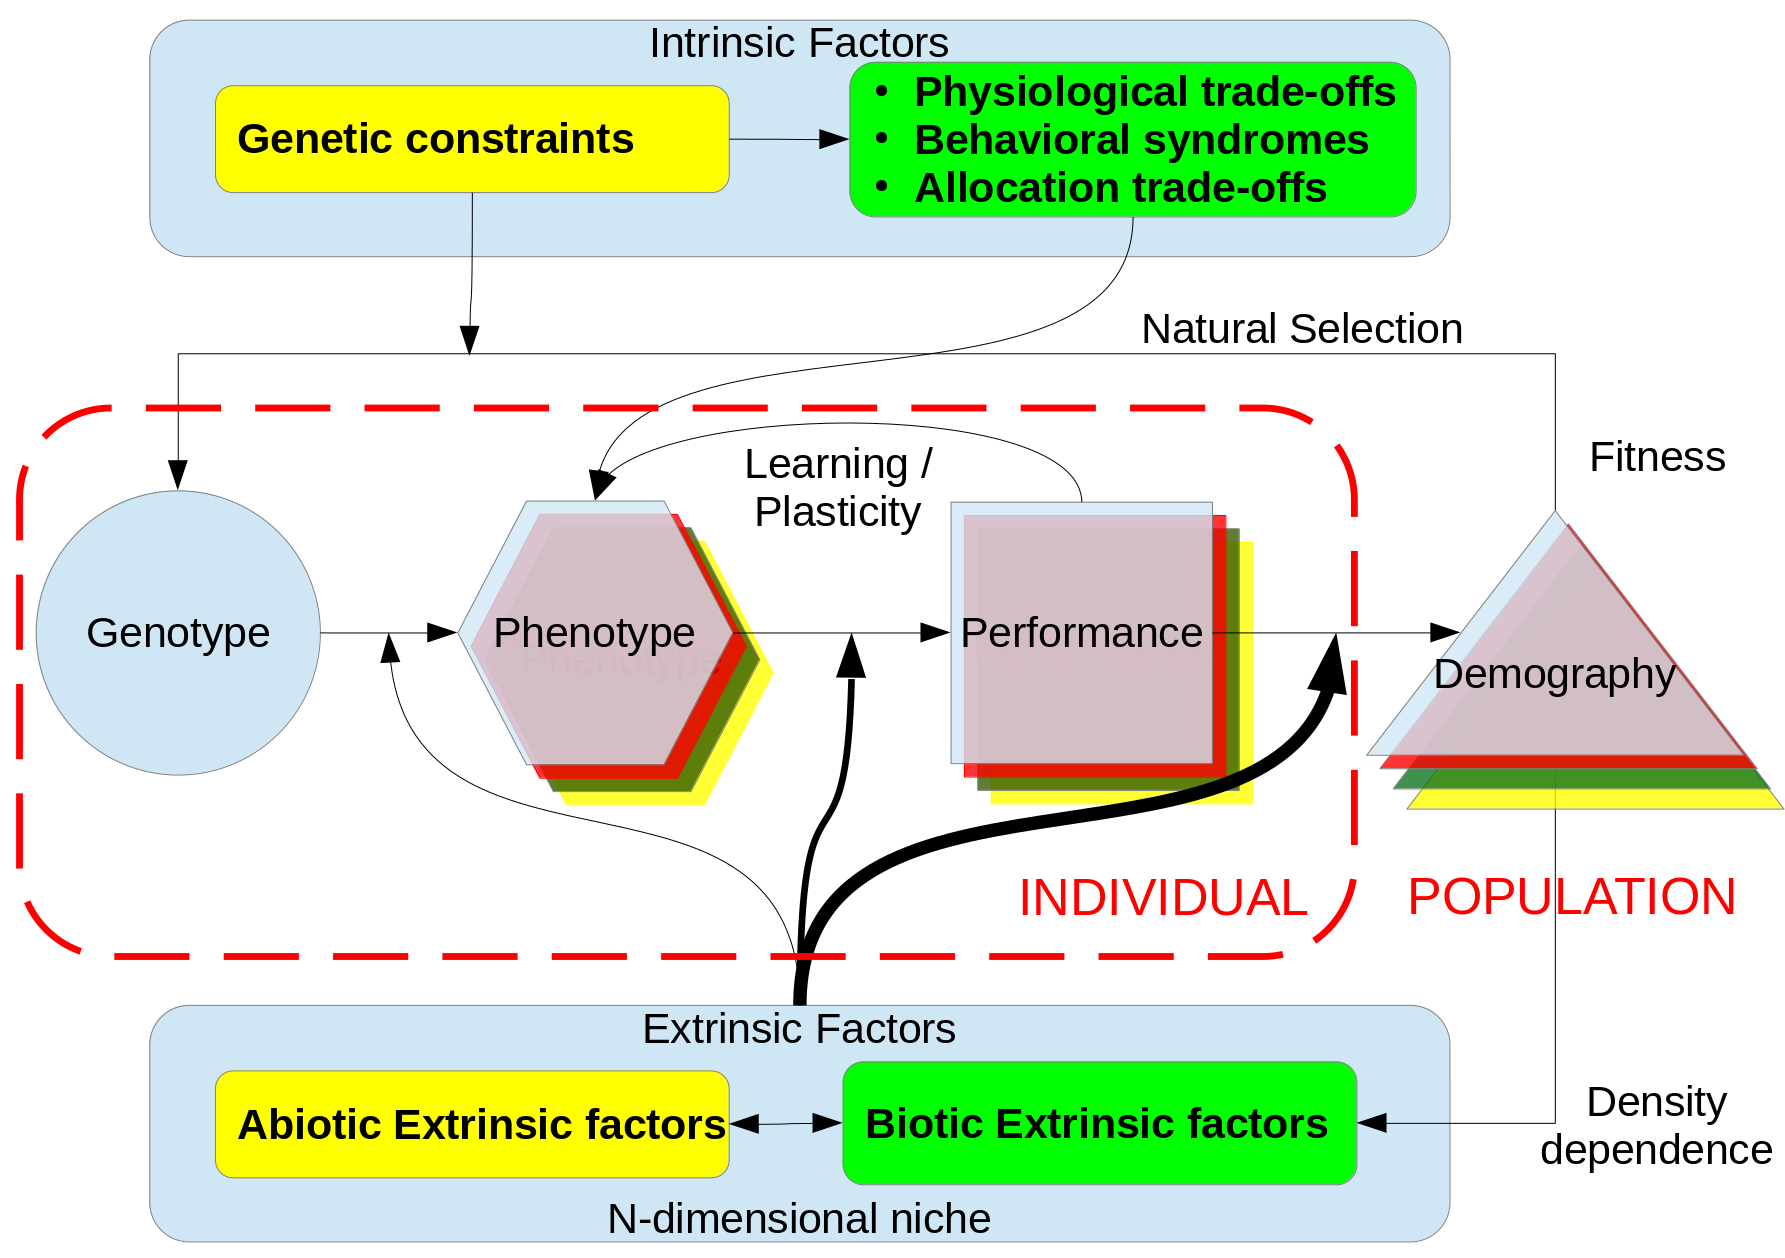
\includegraphics[width=\textwidth]{./Figures/intro/esquemaLH.png}
\caption[LH schema]{
Schematic representation of the life history theory framework with the
different levels of organisation and their relations.
The life history of an individual depends on a series of steps from the
genotype to the phenotype, which then interact with the environment resulting
in a specific performance in terms of reproduction and survival. The effect of
the environment exerts a greater influence at each step modifying the phenotype
and the performance of the individual and ultimately, at the population level
modifying the fitness and the age structure.
At the same time, differential fitness among genotypes change their frequency
in the population by natural selection resulting in evolutionary change. A
second feedback in the system is the influence of organisms and population
on the environment by modifying the population density for the same
species or other species being relevant as preys or predators. Any change
modifying the age-specific mortality will result in a change in the optimum
life history strategy. Inspired by \citet{Ricklefs2002}.
}
\label{fig:fig1.1}
\end{figure}


Despite the seducing philosophy described by \citet{levins1985}, pragmatism and
the need to put limits to this thesis, impose to focus in a subset of the
framework. I choose to focus in the phenotype and demography.
To characterise the phenotype I use the life history traits, individual traits
with direct effects on fitness such as clutch size, age at first breeding or
number of broods per year. I don't consider the intraspecific variation, the
traits were aggregated at species level.
The demographic traits are the population level features affecting
the growth rate such as age-specific mortality rate or average fecundity and
also were aggregated at species level. No evolution nor temporal variation was
considered for the life history traits nor for demographic traits.
Regarding the environmental change, I used data to compare urban and non-urban
areas (Chapter \ref{ch:POLS}) and simulated the effects of unknown new
habitats or resources with better or worst juvenile or adult survival (Chapter
\ref{ch:LH-Behaviour model}).


\section{Life history and behavior}

Behaviour mediates how animals interact with their environment and, by virtue
of their plastic nature, can modify the nature of these interactions, shaping
the biotic and abiotic pressures that act upon them
\citep{Futuyma1988,Losos2004}.

The idea that behaviour, through cognitive and neural machinery, allows
behavioural solutions to unusual or new problems to be devised is known as the
cognitive buffer hypothesis \citep{Allman1993,VanSchaik2003,Sol2009,Sol2009a}.


\begin{small}
\begin{framed}
\subsection*{Box 2: Behavioral Plasticity}

The behaviour can be defined as the actions or inactions of organisms that
change their relation with the environment as a response to external or
internal stimuli. As such, it is a form of phenotypic plasticity. We can
distinguish two types of behavioral plasticity: activational and developmental
plasticity.

\subsubsection*{Activational Plasticity}

Activational plasticity refers to the expression of behaviour and describes the
innate response to stimuli that triggers a shift to an alternative behaviour
through the activation of a neural network \citep{Snell-Rood2013}. Because of
its immediacy and reversibility, such forms of plasticity allow individuals to
rapidly respond to environmental uncertainties by enabling rapid modulation
of, or transitions between, behaviours as a function of the individuals’ needs
\citep{Snell-Rood2013,Sol2013a}. This kind of pre-established responses can be
maladaptive if the individuals face new conditions for which no evolutive
selection has taken place, leading to a so called ecological traps
\citep{Kokko2001}.

\subsubsection*{Developmental Plasticity}

Animals can confront novel challenges, like the need to obtain new types of food
or avoid unfamiliar predators, by modifying or inventing new behaviours, a
process known as developmental behavioural plasticity \citep{Snell-Rood2013}.
Developmental behavioural plasticity is not so immediate as activational
plasticity, because it involves changes in the nervous system that alter motor
responses. However, it has the advantage that it allows animals to construct
responses to unfamiliar or novel problems. One of the main mechanisms behind
developmental behavioural plasticity is learning, the acquisition of new
information influencing performance in behaviour \citep{Dukas1998}. Instead of
consistently expressing the same behaviour to a particular stimulus, learning
allows animals to devise innovative behavioural responses or to improve already
established behaviours on the basis of experience
\citep{Lefebvre1997,Dukas1998,Reader2002,VanSchaik2003,Ricklefs2004}. Learning
is particularly relevant in facilitating the responses to environmental changes,
including new resources, predators or habitats.
\end{framed}
\end{small}


As I argue in this thesis, if we want to fully understand how life history
affects the population dynamics of animals exposed to environmental changes, we
need to explicitly consider the role of behaviour. The argument for the need
to better integrate behaviour into life history theory is founded upon three
main principles.
The first is the fact that behavioural responses are part of the adaptive
machinery of animals to cope with uncertainties and evolutionary disequilibria
of novel environments. While the idea is not new \citep{mayr1965}, recent
theoretical and empirical advances provide a strong foundation for moving
forward \citep{Sol2020, Ducatez2020}.
The second argument is the growing evidence that behaviour affects and is
affected by life history, which implies that both are part of a same adaptive
strategy \citep{Ricklefs2002,Reale2010a,Sol2016,Sol2016a}. When behaviour
change the relations of the individuals with the environment, the age-specific
mortality and therefore the optimum life history strategy also change. Thus,
when we examine how life history affects population dynamics, including
extinction or colonization, we are considering not only life history mechanisms
but also mechanisms related to behavioural responses to novel environments
\citep{Sol2016}.
The last argument is that behaviour mediates some life history mechanisms of
response to novel environments, particularly those related to environmental
uncertainty and adaptive mismatch. For example, to breed or not to breed is a
behavioural decision with direct effects in the number of eggs produced in a
year.
By clearly delineating these mechanisms, we can better infer when it is
necessary to consider behaviour to understand how life history affects the
response to environmental changes.


\section{Objectives}

In my thesis I addressed fundamental unresolved questions about the 
interaction of life history and behaviour in facilitating or impeding the 
response to rapid environmental changes. Chapter \ref{ch:LHaxes} describes the 
main axes of life history traits variation in birds. Chapters
\ref{ch:LH-Behaviour model} and \ref{ch:POLS} explore the links between life
history and behavior, the first using a theoretical model focused on the process
of colonization of novel environments to better understand the mechanisms, and
the second analysing empirical data using comparative methods from urban and
non-urban populations looking for patterns relating life histories and behavior.
The specific goals of the chapters are:


\begin{itemize}
\item \textbf{Chapter \ref{ch:LHaxes}: To describe the axes of life history 
variation in birds}

Not all combinations of life history traits exists in the nature. The traits
covaries due to trade-offs and are organized among different axes. A major axis
of variation of the life history traits is the so-called fast-slow continuum,
which mainly reflects a fecundity-survival trade-off. However, defining and
quantifying the fast-slow axis has proven to be difficult and at least 18
studies have attempted to characterise the fast-slow axis in the last 40 years
with no clear consensus regarding the life history traits that best define it.
I tried to address this problem by giving a demographically meaningful
definition to the axis and identifying the combination of traits that better
describe the underlying trade-off.
In this chapter, I defined the fast-slow axis that better predicts the 
elasticity of the adult survival and generation time from available demographic 
models and a large dataset of life history traits of birds, and describe other
less studied axes of life history from the remaining variation such as the
degree of iteroparity, the relative egg size or the lifelong productivity. Then,
I generated a a global dataset for birds with the position of each species along
the new fast-slow axis, which then can be used for comparative analyses (see
Chapter \ref{ch:POLS} for example).
\bigskip


\item \textbf{Chapter \ref{ch:LH-Behaviour model}: To explore the mechanisms 
linking life history and behavior}

I developed a theoretical individual based model simulating the introduction of
a species with different life histories in a new environment with different
habitat options characterized by different degrees of habitat mismatch that
affects adult or juvenile mortality and evaluate how the life history and
behaviour could interact and affect the persistence of the population under
stochastic and maladaptive scenarios. Specifically, I tested 6 different
behaviours representing activational plasticity affecting preferences for the
best habitat or the worst (ecological trap) or skipping a reproductive event
when individuals are on the worst habitat, and behaviours representing
developmental plasticity by increasing the probability to change habitat
when there is a breeding failure or by learning by exploring, and a neutral
choice behavior.
\bigskip


\item \textbf{Chapter \ref{ch:POLS}: To analyse the effects of life history and 
behaviour in the ability to colonize urban habitats}

By means of a comparative analysis of flight initiation distances (i.e., the
distance at which an animal takes flight when a human being is approaching)
across \textgreater{300} bird species distributed worldwide, I show the
existence of a peace-of-life syndrome (POLS) predicted by theory where
slow-lived species tend to be more risk-averse than fast-lived species.
Furthermore, the POLS structure vanishes in urbanized environments due to
slow-lived species adjusting their flight distances based on the perception of
risk showing that slow species have a more plastic behaviour which can
potentially facilitate the adaptation to environmental changes.
\end{itemize}

\bigskip


Hopefully, this thesis will contribute to develop a new way to understand how
life history influences population growth in novel or changing environments,
potentially contributing to a more predictive theory. Such a theory may be
useful to help prevent and mitigate the ecological and economic impact of
biological invasions \citep{Kolar2002, Vall-llosera2009, Leung2012}. The new
theory should also be of great importance in predicting extinction risk
associated with human-induced rapid environmental changes like habitat
destruction and climate change \citep{Saether2000, Sih2011}.

%TODO: References & add figures and tables
% check comments on /home/joan/Documents/owncloud/doctorat2/projectes/LHT/axis/MS-v11.odt
% check FS vs fast-slow nomenclature
%************************************************
\chapter[Axes of life history variation]{Revisiting the fast-slow continuum of 
life history variation in birds}\label{ch:LHaxes}
%************************************************

% \tikz[remember picture,overlay] \node[opacity=0.3,inner sep=0pt] at (current page.center){\includegraphics[width=\paperwidth,height=\paperheight]{./Figures/cover/Goya_Dog.jpg}};
%\tikz[remember picture,overlay] \node[opacity=0.3,inner sep=0pt] at ([yshift=6cm]current page.center){\includegraphics[width=\paperwidth,height=\paperheight]{./Figures/cover/Goya_Dog.jpg}};
\clearpage

\section*{Abstract}

Despite overwhelming evidence that the life history of organisms has diversified
in a broad variety of combinations of reproduction rate, age at maturity and
longevity, it is still uncertain what combinations of life history traits are
possible in nature. Here, we use an unusually large dataset of life history
information for birds to demonstrate that not all combinations of life history
traits are possible. Rather, much of life history variation is structured along
the fast-slow continuum, defined on the basis of elasticity analyses and
estimations of generation time derived from demographic models. The fast-slow
continuum may be best described by $\sim70$ (elasticity) or $\sim500$
(generation time) out of 7527 possible trait combinations, is only weakly
correlated with body mass and exhibits substantial phylogenetic signal. After
extracting the fast-slow continuum, the remaining life history variation is
structured along other less studied axes defined by the frequency of
reproductive bouts, the extent of developmental period and the quality-quantity
trade-off in egg production. Describing the fast-slow continuum based on
demographic analyses avoids the vagueness of the concept and allows integrating
it with other axes of variation, providing a more solid basis to continue
investigating the causes and consequences of life history variation through
broad comparative analyses.


\section{Introduction}

Life history defines how organisms allocate their limited time and energy to
reproduction and survival \citep{stearns1992evolution}. Early works demonstrated
that the life history of organisms has diversified in an extraordinary variety
of combinations of reproduction rate, age at maturity and longevity, reflecting
the existence of trade-offs and constrains. However, it is  still uncertain
what combinations of life history traits are possible, and why some strategies
have achieved greater evolutionary success. Documenting how life history
varies across organisms is of interest in itself, and also because population
dynamics ultimately depend on how organisms allocate their limited time and
energy to reproduction and survival \citep{stearns1992evolution}. Consequently,
life history traits have a great potential to influence key ecological and
evolutionary processes, such as the likelihood of colonising new areas, the risk
of extinction and the rate of evolutionary change (see
\citet{stearns1992evolution,roff1992evolution,roff2002}).

In the last 40 years, at least 18 studies have attempted to characterize the
main axis of life history variation across species. These works use empirical
data for a set of life history traits to describe the covariation between them.
Despite the differences on the methods and taxa used all studies are consistent
on defining a “slow-fast” axis, a term first used by \citet{Stearns1983a}.
The fast-slow continuum has attracted considerable attention because it is
predicted by the age-specific mortality theory of life history evolution
\citep{Stearns1977,Charlesworth1980}⁠ and because it has implication in
understanding how organisms respond to environmental changes.

The challenge of understanding what combinations of life history traits are
possible is exemplified by the unsettled controversy about how to quantify the
fast-slow continuum axis of life history variation across species. The fast-slow
continuum aligns organisms along an axis from a “high reproductive-short life
expectancy” (fast-lived) strategy at one end to a “low reproductive-long life
expectancy” (slow-lived) strategy at the other end. Despite being one of the
most studied and influential axes of life history variation, there are notorious
discrepancies regarding how to define and quantify it across species. Indeed, at
least twelve different life history traits have been used to this purpose either
alone or in combination
% TODO: fix table \ref{tab:tabApp2.1.1} or remove reference
%(Table \ref{tab:tabApp2.1.1}),
often being chosen based on data availability rather than on biological
significance. For example, many studies describe the fast-slow continuum based
on surrogates of fecundity like clutch, litter size or productivity, ignoring
that a high reproductive effort has high costs in terms of survival
\citep{Adler2014}. Inconsistencies in the treatment of body size in previous
studies have also been shown to profoundly affect the quantification of the
fast-slow continuum \citep{Jeschke2009}.
Although many life history traits scale with body size, it is unclear whether
body size should be considered part of the fast-slow continuum (e.g. because
being larger improves survival) or should instead be factored out because it
merely represents constrains (e.g. it takes longer for larger organisms to
develop than it does for smaller organisms). The vagueness of the fast-slow
continuum makes the concept and its ecological and evolutionary implications
difficult to evaluate \citep{Jeschke2009}, and limits our capacity to identify
independent axes of life history variation.

The difficulties regarding how to define the fast-slow continuum across species
may come as a surprise given that early works are clear in describing it as the
result of the impossibility to simultaneously maximize survival and fecundity
\citep{Stearns1983a, Saether1988}. This means that the fast-slow continuum needs
to be understood in the context of the full lifecycle of a species. The
assessment of the relative sensitivity (i.e. elasticity) of population growth to
changes in fecundity and adult survival may be useful for this purpose, as it
helps describe the fecundity-survival trade-off. Thus, a slow-lived strategy
should be characterised by high elasticities for adult survival and low
elasticities for fecundity, the contrary being true for fast-lived species.
According to \citet{Gaillard1989}, the fast-slow continuum can also be 
represented as a time scale gradient ranking species according to turnover (see 
also \citet{Jeschke2009,Saether2013,Adler2014}⁠). Under this view, the
fast-slow should be better characterised by estimating generation time, where a 
long generation time is a distinctive feature of slow-lived strategies.

While demographically-derived approaches to the fast-slow continuum represent
important advances, resulting in metrics that are more accurate and
demographically meaningful, the paucity of information of species’ life cycles
limits their application to broad comparative analyses that are geographically
and taxonomically representative. This severely limits our capacity to discern
what combinations of life history traits are possible in nature. One way to
overcome such a limitation is to use a demographically-derived approach to
identify the combinations of life history traits that best predict either
generation time or the fecundity-survival trade-off (i.e. elasticities of
fecundity and adult survival), and then use the best combinations to estimate
the position in the fast-slow continuum of species for which information of the
full life cycle is not available.

In the present paper, we use this framework to characterise the fast-slow
continuum of birds, a group that has played a pivotal role in developing life
history theory but for which characterizing the fast-slow continuum has proved
particularly difficult. We first estimate elasticities for adult survival and
generation time for a subset of species for which demographic data are
available. We then explore the extent to which all the combinations of the 14
life history traits most commonly used to describe the fast-slow continuum 
predict variation in elasticities and generation time. Once the best 
combinations of traits are identified, we use them to classify 
\textgreater{1000} species along the fast-slow continuum.

We finally investigate the life history variation that remains once variation
in the fast-slow continuum is factored out, and describe three extra axes
related to iteroparity, development time, and the quality-quantity trade-off for
the offspring.


\section{Methods}

\subsection*{Life history traits}

We assembled published information on the 14 life history traits most often used
to describe the fast-slow continuum (Table \ref{tab:table2.1}). These traits
describe adult quality (LFS, RLS, AFB), juvenile quality (DP, I, FLE, EMR,
OV), and the number of offspring (FEC, CS, PRO, PEP), iteroparity (BV), and body
mass (BM). We found information of the 14 life history traits for 
\textgreater{6700} species (full life history dataset; see Table 
\ref{tab:table2.1} for details), and complete information for 797 species 
(restricted life history dataset). All traits were log-transformed except BV, 
OV and EMR.


\begin{table}
\caption[Life history traits]{Life history traits considered in the present
study. Sample size is the number of species for which information is
available.}\label{tab:table2.1}
\begin{tabular}{@{}p{2.5cm}cp{7.5cm}p{1.5cm}@{}}
\toprule
Trait                         & Abbreviation & Definition                                   & Sample size \\
\midrule
Maximum lifespan              & LFS          & Maximum recorded lifespan                    & 1583        \\
Maximum reproductive lifespan & RLS          & LFS - AFB                                    & 1088        \\
Age at first breeding         & AFB          & Age at which individuals start reproducing   & 1205        \\
Developmental period          & DP           & Period from egg laying to fledging (I + FLE) & 1907        \\
Incubation                    & I            & Period from egg laying to hatching           & 2577        \\
Fledging                      & FLE          & Period from hatching until fledging          & 1980        \\
Egg mass residual             & EMR          & Relative egg mass                            & 4074        \\
Fecundity                     & FEC          & $CS$ multiplied by the number of broods per year         & 1633 \\
Clutch size                   & CS           & Number of eggs in a given clutch             & 6551 \\
Productivity                  & PRO          & Egg mass * fecundity / body mass             & 1582 \\
Potential Egg Production      & PEP          & $PRO * RLS$                                  & 901 \\
Brood value                   & BV           & $log10\left(\tfrac{1}{ broods \cdot RLS } \right)$       & 909  \\
Offspring value               & OV           & $log10\left(\tfrac{1}{ FEC \cdot RLS } \right)$          & 909 \\
Body mass                     & BM           & Weight                                       & 6462        \\
\bottomrule
\end{tabular}
\end{table}

\subsection*{Restrictions in the life history traits space}

With our life history dataset, we first investigated which portion of the 
dimensional trait space is occupied by birds that nowadays live on Earth. We 
restricted this analysis to 9 life history traits (LFS, EMR, BM, DP, FLE, 
AFB, CS, FEC, BV), to avoid redundancies and to reduce the computational cost, 
and used them to compute a nine-dimensional convex hull volume containing 95\% 
of the observed combinations of the traits. The volume of the hull 
was compared with mean hypervolumes generated from 4 null models randomised 
999 times ($hv_{nm}$ hereafter), following \citet{Diaz2016}⁠. 
Hypervolumes in $hv_{nm1}$ to $hv_{nm3}$ assume that the traits vary 
independently. Null model 1 assumes that any combination of trait values can 
exist with equal probability, each trait having a uniform distribution 
approximating an hypercube. Null model 2 assumes that extreme trait values are 
selected against during evolution and each trait has a normal distribution, 
with hvnm2 approximating an hypersphere. Null model 3 imposes no assumptions 
about trait distributions but instead allows each trait to be distributed as 
observed and assumes traits are independent of each other. Null model 4 assumes 
that extreme values are selected against (i.e., normally distributed) and 
maintains the observed correlation structure among traits. Relative to null 
models 1 to 3, null model 4 collapses the multidimensional trait-space occupied 
by birds (hvnm4) into an elongated hyperellipsoid.


\subsection*{Identifying the life history traits that best describe the 
fast-slow continuum}

We used the COMADRE Matrix Database Version 4.20.11.0 
\citep{Salguero-Gomez2016} to obtain age-structured population models that 
incorporate accurate information on the rates of survival, growth, and 
reproduction for 174 bird populations belonging to 78 species (demographic 
dataset, hereafter). For each species we selected population matrices from 
wild, unmanipulated populations with complete data instead of pooled from 
different populations if available (n = 42). See figure \ref{fig:fig2.1} to 
compare the distribution of the life history traits using the restricted 
dataset and the subset with demographic data from the population matrices.

\begin{figure}
\centering
\includegraphics[width=\textwidth]{./Figures/chapter02/fig1-LH_demo_traits.png}
\caption[Traits distribution]{
Biplots (upper triangle) and density plots (lower triangle) of the traits. 
Black for species with either demographic or traits data and red dots for 
species with both demographic (gen.T for generation time and elas.A for 
elasticities to adult survival) and life history traits data (see table 
\ref{tab:table2.1} for details).}
\label{fig:fig2.1}
\end{figure}

From each population matrix model, we calculated 2 demographic 
traits \citep{Caswell2001,Stubben2007}: generation time and elasticity of the 
adult survival. The elasticity matrices show the proportional effects on 
population growth rate for each demographic trait \citep{deKroon2000}⁠. We 
selected elasticities for adult survival and net fecundity as a measure of the 
importance of these components on the life history strategies. However, both 
elasticities were perfectly correlated (correlation coefficient = 1) and we only 
used the elasticities of the adult survival.

To assess how well life history traits correlate with the estimated demographic 
traits, we used the 14 life history traits previously described (Table 
\ref{tab:table2.1}), which were available for the 30 species. The estimated 
elasticities and generation times were modelled as a function of life history 
traits by means of phylogenetic least square regressions (with Pagel’s 
$\lambda$ estimated by means of maximum likelihood), as implemented in the R 
package “phylolm” \citep{Ho2014}⁠. The traits were tested alone and combined 
with other traits by means of phylogenetic principal component analysis 
(PPCA), with maximum likelihood estimates of $\lambda$, as implemented in 
“phytools” \citep{Revell2009a}⁠. The phylogenetic analyses were run with 
2 consensus trees from \citet{Jetz2012}, one for the Ericsson and 
one for the Hackett backbones.
The PPCAs were obtained using the restricted life history dataset (n = 797). We 
assembled all combinations of traits with the only rule that a PPCA should 
include at least a trait related to adult quality, juvenile quality and the 
number of offspring. A total of 10080 combinations of traits were used in the 
PPCAs, from which 2464 were discarded due to unsatisfactory convergence, 
resulting in 7616 trait combinations with a proper PPCA. For each PPCA, we 
selected the Principal Component (PC) that better match the demographic traits 
($\Delta AIC = 0$) and flipped the axis when 
needed, multiplying the PC scores and loadings by -1 in order to sort the 
species from fast (negative values) to slow (positive values).

From all the studied traits, whether alone or combined in a PC, we 
considered those that better explain variation in elasticities or generation 
time as corresponding to the fast-slow axis. We tested their relative 
importance by estimating the AIC based weight of each regression, considering 
the best models as those with 2 units difference from the model with the lowest 
AIC ($\Delta AIC < 2$).


\subsection*{Defining species position on the fast-slow axes}

Our previous analyses are based on the combination of detailed demographic data 
and full life history information for 30 species. If there are combinations of 
life history traits that accurately predicts variation in elasticities and/or 
generation time, it is possible to use the life history information to assess 
the position in the fast-slow continuum for species for which demographic data 
was unavailable. We defined the position of the species in the fast-slow axis 
as the mean scores of the PCs weighted by the AIC based weights 
of the elasticity models (FSe) and generation time models (FSgt). We did the 
same using all selected PCs and using only the PCs of the best models only 
($\Delta AIC < 2$).

Our finding that to accurately predict elasticities and/or generation time you 
only need a few life history traits, not all of them, open the possibility to 
assess the position in the fast-slow continuum for many more species than those 
with full information on the 14 key life history traits. Therefore, we repeated 
each of the PPCAs identified as best predictors of elasticities and generation 
time in the previous analyses, but now including all the species for which 
information on the underlying life history traits was available, regardless that 
other traits were missing. As before, we defined their position as the mean 
scores of best PCs weighted by the AIC based weights of the elasticity 
and generation time models (FSe and FSgt).

Our extrapolations to estimate the fast-slow axes assumes that the studied
subsets of species are representative of the observed variation in the fast-slow
continuum.
This assumption is supported by two analyses. First, the phylogenetically 
corrected correlation \citep{Revell2009a}⁠ of the relevant PCs estimated with
the demographic, restricted and full life history datasets was
\textgreater{0.99} in all cases.
Second, the mean values of each PC estimated for our subsets of species (i.e.
the demographic and restricted datasets) do not significantly differ from those
expected by randomly sampling the same number of species from the full life
history dataset.


\subsection*{Other axes of life history variation}

We analysed the remaining ~9500 (from 9385 to 9604 depending on the life 
history dataset and phylogeny) significant PCs (eigenvalue \textgreater{1}) not 
selected as components of the fast-slow axes to explore potentially different
axes of variation. First, we used the correlation among the scores of the PCs to
build clusters using different minimum absolute correlations (0.7 – 0.9),
discarding clusters containing less than 5\% of the PCs and removing duplicated
clusters in different correlation thresholds.
For each group, we flip the PCs to align the scores and loadings when needed. 
Every cluster represents a potential axis of life history variation. We grouped 
clusters with a correlation on averaged loadings \textgreater{0.95} for 
visualization purposes.


\subsection*{Characterisation of the life history axes}

For each potential axis, we calculated the mean and the standard deviation of 
the loadings multiplied by the relative frequency of the traits. As the 
frequencies of the traits were not the same for each cluster, we also estimated 
the relative weight of each trait as the proportion of the absolute values of 
the loadings in a PC minus the relative frequency of the traits in the PC 
cluster. The relative weight of the traits ranges from -1 to 1, where negative 
values means that the absolute value of the trait loadings are lower than 
expected by the frequency of the trait and positive values for traits with 
higher loadings than expected by the frequency of the trait. In addition, we 
calculated the part of the variance explained by each PC from the total variance 
of the traits included in the PPCA.
For the fast-slow axes we weighted the former metrics by the AIC based weight
from all the models and also including only the best models.

For each defined axis, we averaged the scores of the species to generate a data 
base of life history for birds. Again, for the fast-slow axes we weighted the
PCs scores by the AIC based weight for all models and also using the PCs in the
best models only. The averaged scores of the fast-slow axes where then used to
predict adult elasticities and generation time to compare the performance
against the scores of single PCs.


\section{Results}

The observed hypervolume based on the 9 non-redundant life history traits is 
much smaller than the hypervolumes predicted by the null models (p-value = 
0.001, see table \ref{tab:table2.2}). The closest null model, $hv_{nm4}$, is 
the one that imposes a correlation among traits as observed but still 7 times 
larger than the hypervolume of the observed data. The smaller size and 
aggregation in the hypervolume indicate that not all trait combinations are 
possible, consistent with the existence of constrains and trade-offs in the life 
history evolution. The observed aggregation of species is greater for the 
observed traits than the expected for each $hv_{nm}$ (table 
\ref{tab:table2.2}). Thus, the existing diversity of life history strategies 
seems restricted to certain combinations of correlated traits and shows a 
greater concentration in the trait space than expected under multivariate 
normality.

\begin{table}
\center
\caption[Species' concentration and hypervolumes]{The world's bird species are
concentrated in nine-trait space as compared to expectations under theoretical
null models and fills a much more restricted hypervolume. Minimum number of 
cells within nine-trait multivariate space (divided in $10^{6}$ cells) needed to
cover 10\% (N10) or 50\% (N50) of species in the observed hypervolume 
($Hv_{obs}$) and in four different null-model simulated hypervolumes 
($Hv_{nm1-4}$) and the volume of each hypervolume (the mean of the 999 
permutations for $Hv_{nm}$). See main text for details.}
\label{tab:table2.2}
\begin{tabular}[b]{@{}lccc@{}}
\toprule
\textbf{Hypervolume} & \textbf{N10} & \textbf{N50} & \textbf{Volume} \\
\midrule
$Hv_{obs}$  & 9   & 71  & 4.3 \\
$Hv_{nm1}$  & 131 & 354 & 1030450 \\
$Hv_{nm2}$  & 131 & 397 & 10808.4 \\
$Hv_{nm3}$  & 131 & 394 & 8187 \\
$Hv_{nm4}$  & 131 & 312 & 30.6 \\
\bottomrule
\end{tabular}
\end{table}

From the 7631 trait combinations, including single traits, the selected PCs 
scores from the PPCAs combining sets of traits, and other metrics used to 
describe the fast-slow continuum in the literature, 104 where among 
the ones that better predict elasticities for adult survival ($\Delta AIC < 2$),
while for predicting generation time 468 trait combinations where among the
bests. All the best predictors are PCs scores except for the single trait clutch
size that is also part of the best predictors for the elasticity of the adult
survival.
The best PCs come from PPCA with $5.9 \pm 1.3$ combined traits for adult 
survival elasticities and $6.2 \pm 1.3$ for generation time. The variance 
explained by the PCs account for $54\% \pm 0.008$ of the variance of the traits 
sets selected for the elasticities of adult survival and $48\% \pm 0.008$ 
for the trait sets selected for generation time. Here we report the results for 
the restricted life history dataset using the phylogeny based on the Hackett 
backbone, see table \ref{tab:tabApp2.1.1} for the details of the extended life
history dataset and the models with the phylogeny based on the Ericson backbone.

Although single traits are often used as surrogate for the fast-slow axis, only
CL appears among the best models for elasticity of the adult survival ($\Delta
AIC = 0.6$ ) and no single trait for generation time (see
\href{https://github.com/jmaspons/Thesis/tree/master/ESM/chapter02}{
FS\_modelSelection.xlsx in the ESM}). The ratio FEC / AFB, which has also been
suggested to accurately describe the fast-slow axis \citep{Oli2004}⁠, is not
among the best traits, alone or in combination, that better explains adult
survival elasticities ($\Delta$AIC = 85.6) nor generation time ($\Delta$AIC =
10.2).

\begin{figure}
\centering
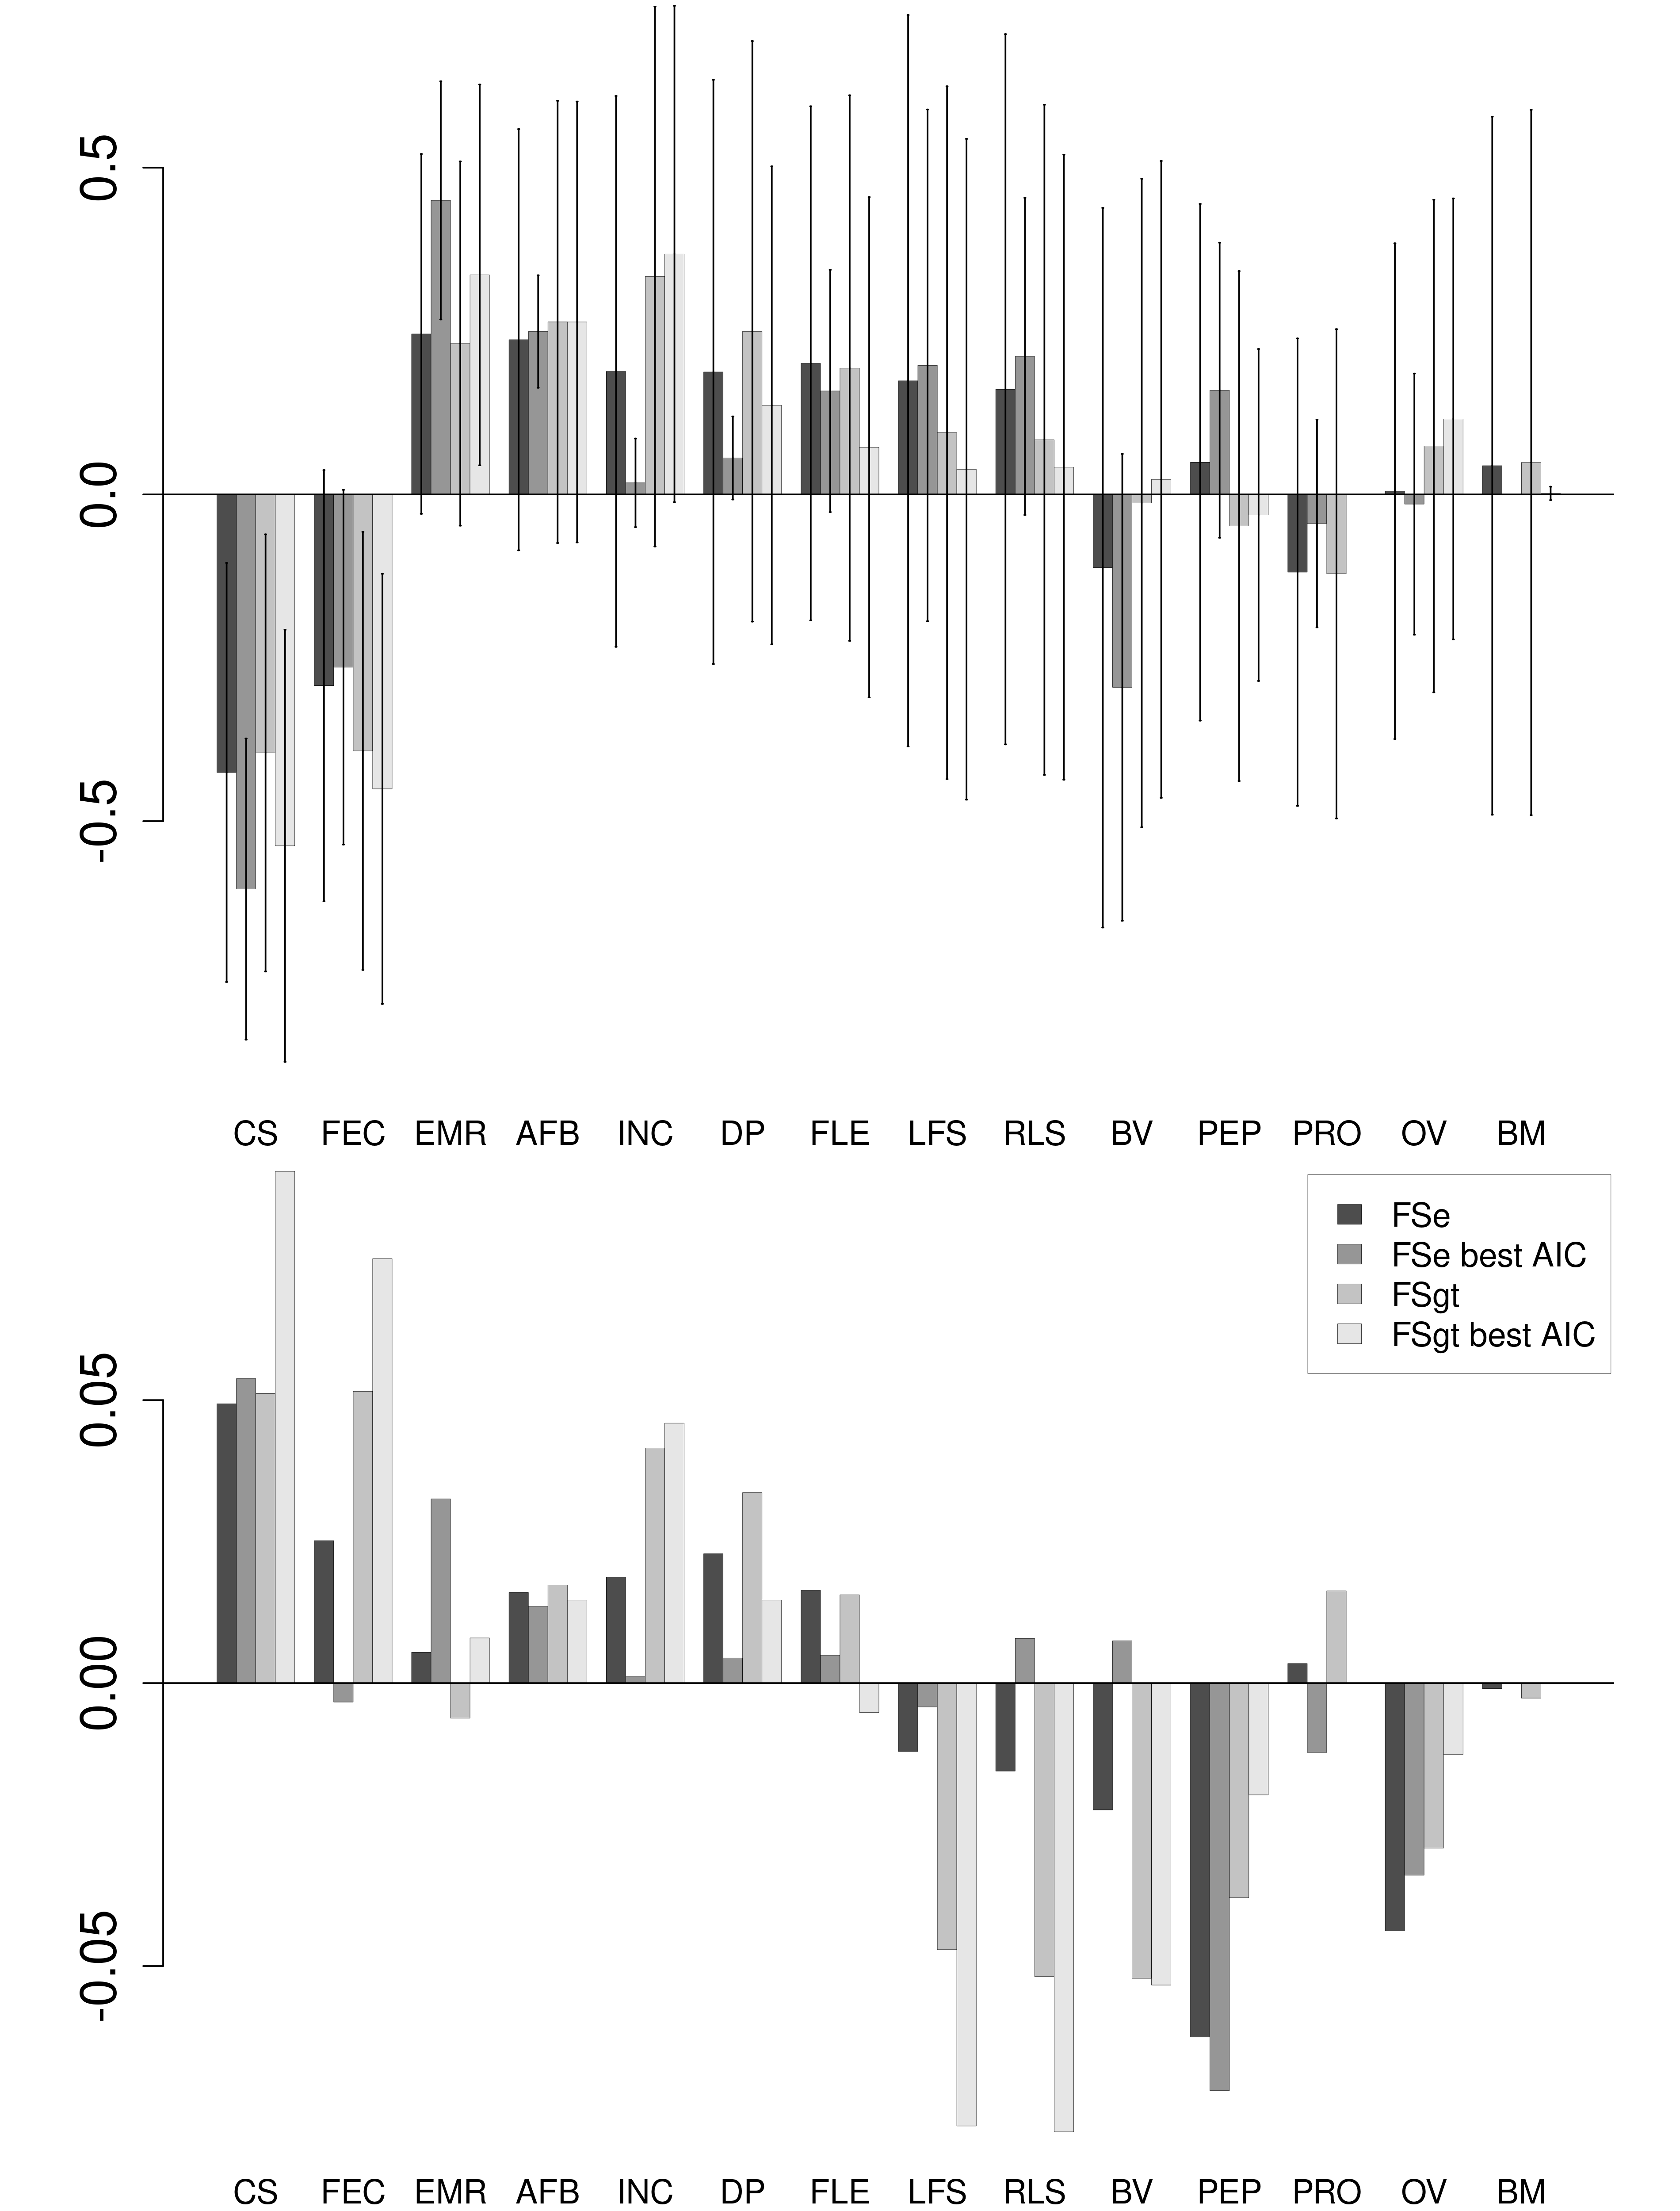
\includegraphics[width=\textwidth]{./Figures/chapter02/fig2-FSaxes.png}
\caption[Fast-Slow PC loadings]{
Importance of the traits describing the fast-slow continuum. Top panel: Loadings 
mean $\pm$ standard deviation of the selected PCs combining sets of life history traits that
better describe the fast-slow axis. Bottom panel: Relative weight of the life 
history traits in the fast-slow continuum. Values range from -1 to 1, where 
negative values means that the absolute value of the trait loadings are lower 
than expected by the frequency of the trait and positive values for traits with 
higher loadings than expected by the frequency of the trait in the selected 
PPCAs (see main text for details). The loadings and frequencies come from the
selected PCs that better predict elasticities of the adult survival (FSe) or
generation time (FSgt), weighted by the AIC based weight of the models taking
all or only the models with $\Delta AIC < 2$ (best AIC).}
\label{fig:fig2.2}
\end{figure}


Figure \ref{fig:fig2.2} shows the loadings of each life history trait in the 
best fast-slow axes, for both elasticities and generation time. In both
cases, the life history traits with higher and consistent weights include CS and
AFB.
However, there are two main differences. First, incubation period is more 
influential for the axis based on generation time than for those based on 
elasticities. Second, FEC seems more important for PCs selected to 
predict generation time. Other traits in selected PCs have huge variability 
(see SD bars in figure \ref{fig:fig2.2} and depends on whether all models or 
only the best ones ($\Delta AIC < 2$) are used to weight the PC. Other traits 
commonly included in the fast-slow axis such as LFS or BM seems unrelated to 
the demographically defined fast-slow axis defined by our methodology. The
results for the extended dataset and the Ericson backbone based phylogeny
doesn't change the patterns (see tables \ref{tab:tabApp2.1.2},
\ref{tab:tabApp2.1.3} and figures \ref{fig:figApp2.1.1}, \ref{fig:figApp2.1.2}).

One advantage of combining all PPCA in single weighted-average axes is that it 
allows to estimate the position of a species in the fast-slow axis even when
some scores cannot be estimated due to missing data for life history traits
combined in a PPCA. We thus estimated the fast-slow continuum for up to 1516
species for each respective axis.
The two estimated fast-slow axes (FSe and FSgt) are highly correlated with each
other (phylogenetic correlation =  0.85 and 0.74 for all or best models
only, n = 797 species), are only weakly correlated with body mass (phylogenetic
correlations = 0.5 and 0.34, respectively) and exhibits substantial phylogenetic
effects ($\lambda > 0.95$).

\begin{figure}
\centering
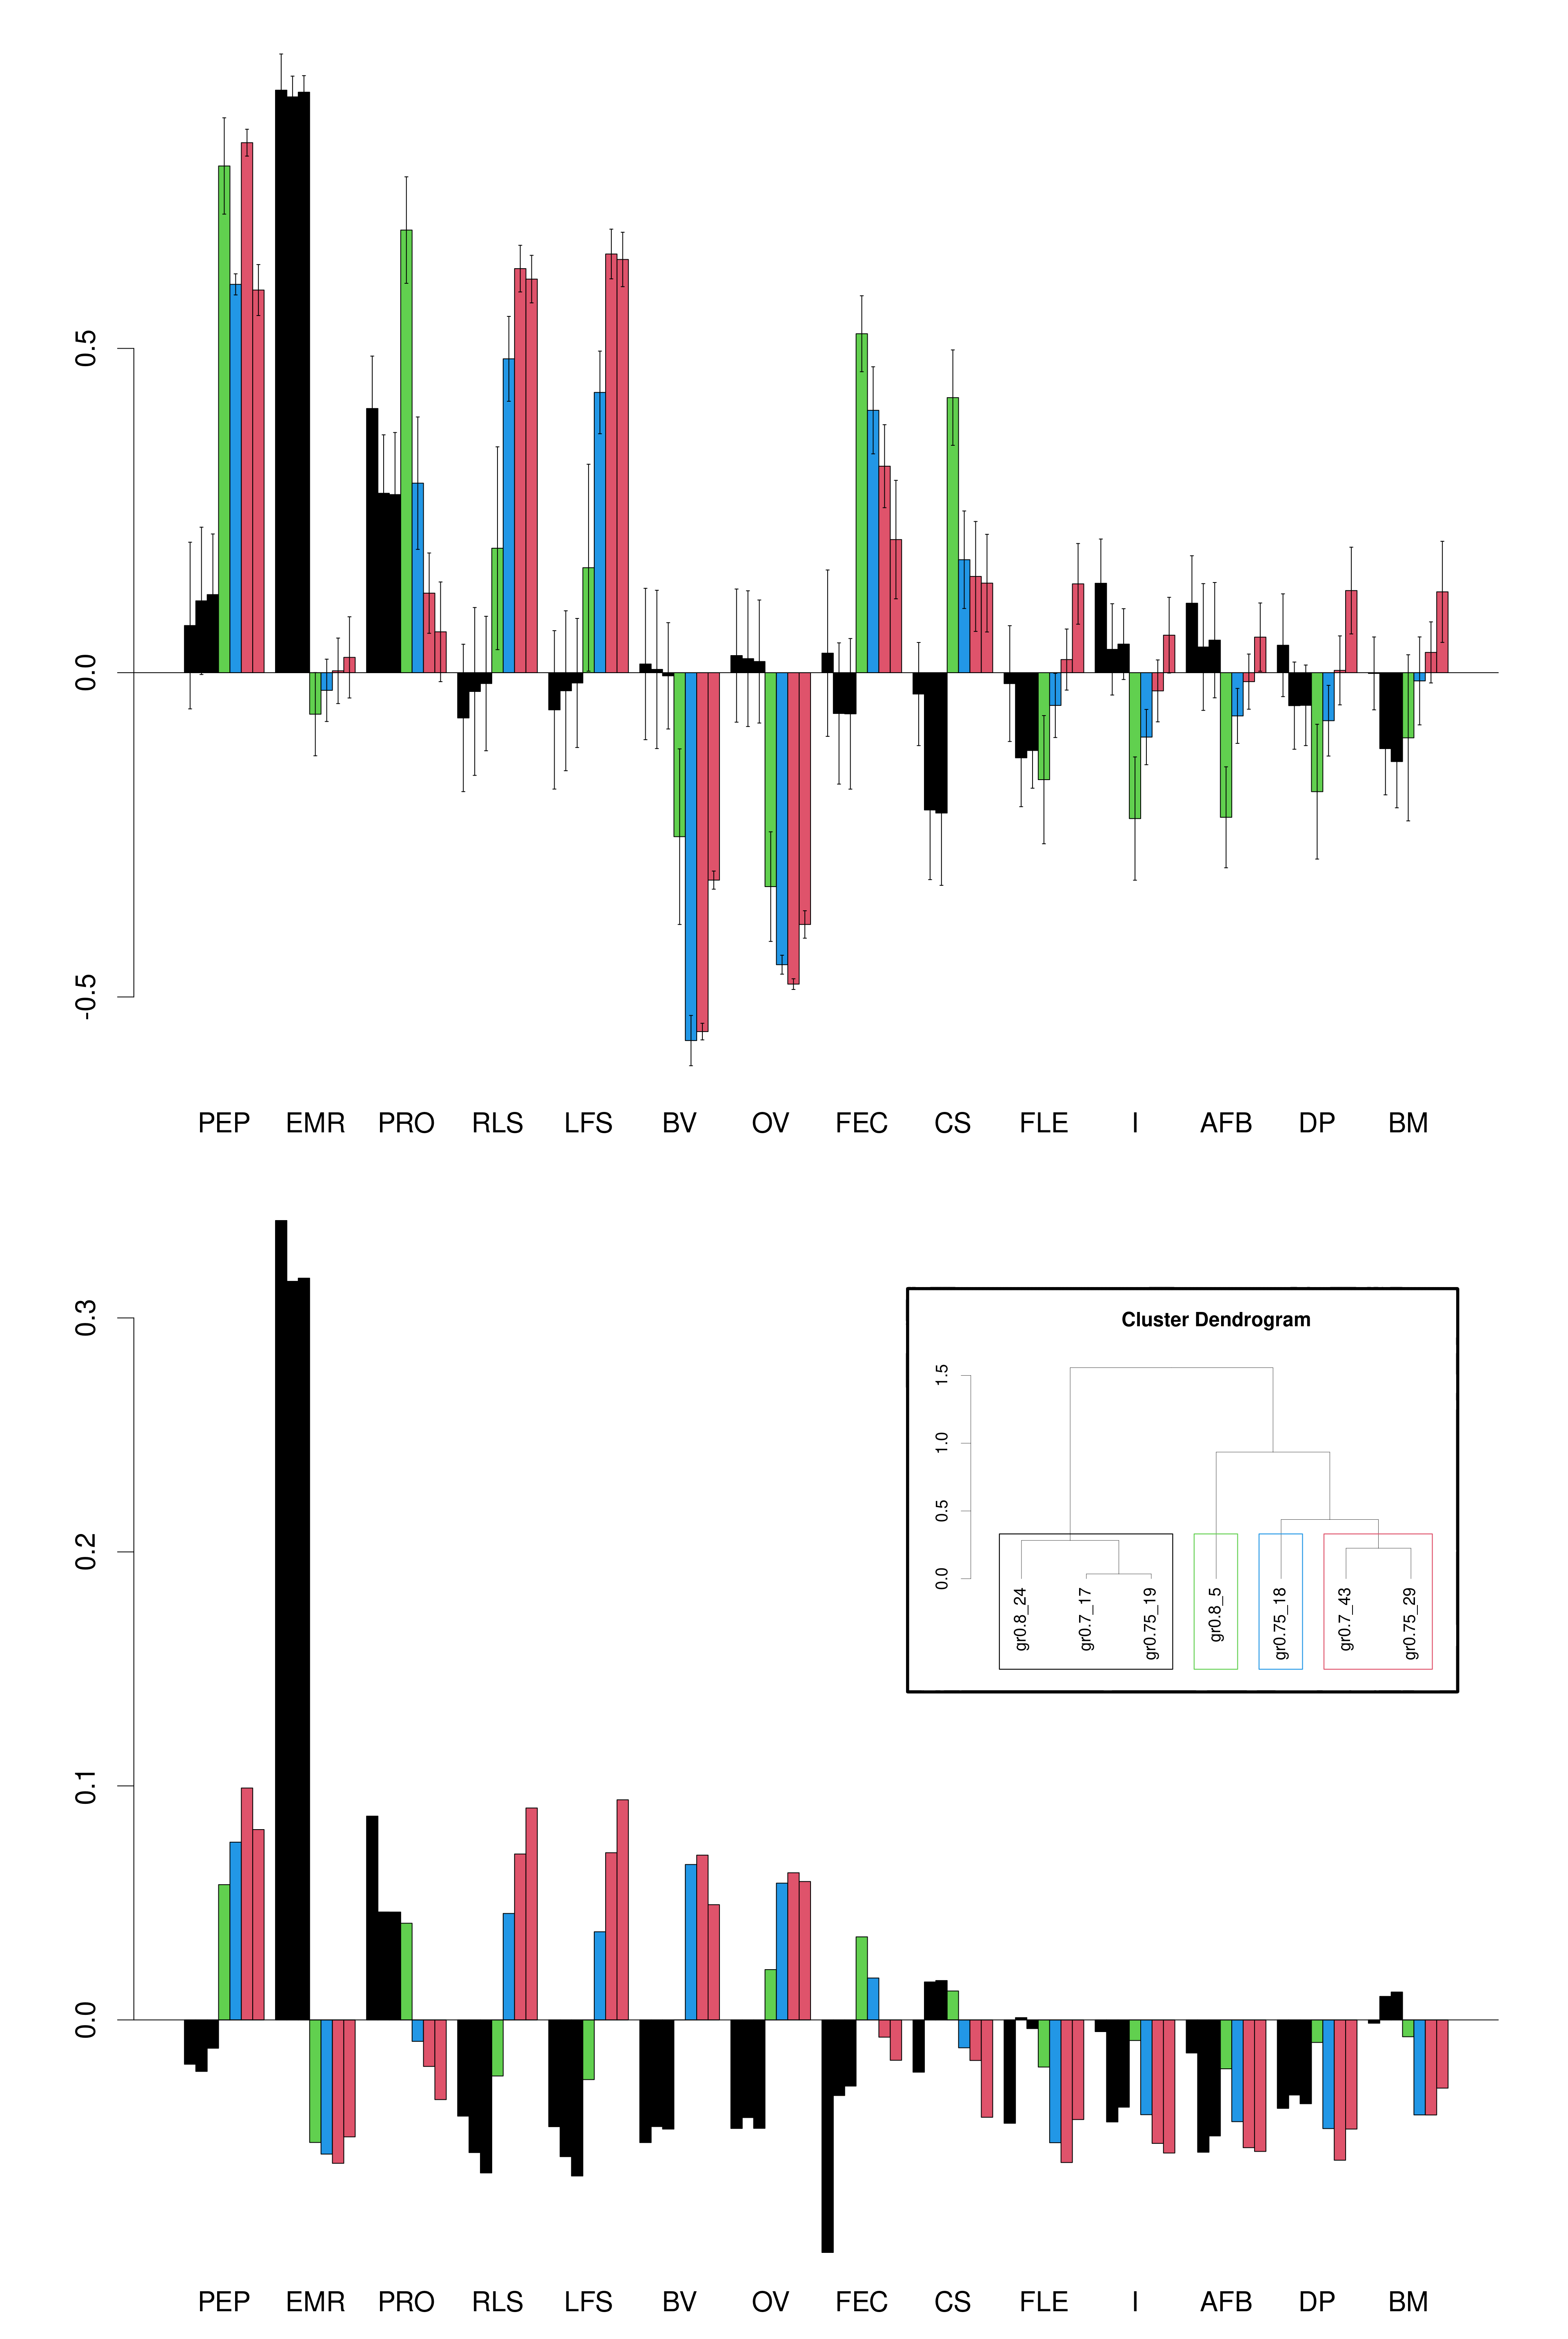
\includegraphics[width=\textwidth]{./Figures/chapter02/fig3-Secondary axes.png}
\caption[Alternative axes groups and PC loadings]{
Importance of the traits for clusters of similar significant PCs not selected
for the fast-slow axes. Each group contains PCs with scores correlation greater
than the correlation specified in the group name in the inset dendogram (e.g.
grCor0.8 means correlation \textgreater{0.8}). Top panel: Loadings mean $\pm$
standard deviation for the traits of each group of PCs. Bottom panel: Relative
weight of the life history for each group of PCs (see figure \ref{fig:fig2.2}
for details).}
\label{fig:fig2.3}
\end{figure}

Although the PCs representing fast-slow continuum explains around 50\% of the 
variation in life history traits, much variation still remains to be explained.
To explore thus variation, we extracted all the PCs with Eigenvalue
\textgreater{1} (Kaiser-Guttman criterion) among the
%TODO: cite Kaiser criterion (Legendre P, Legendre L (2012) Numerical Ecology 
% (Elsevier, London), 3rd Ed, p 1006)
PCs not selected as descriptors of the fast-slow continuum, and classified them
in groups based on a cluster analyses of species scores (fig. \ref{fig:fig2.3}).
These clusters classify together PCs that represent similar life history axes,
which may then be interpreted by examining their traits loadings. The averaged
loadings of these groups suggest at least three axes of life history variation
that are independent of the fast-slow continuum.

% TODO: axes' characteristics
\ref{tab:tabApp2.1.4}

The most important one in terms of variance explained is the degree of
iteroparity (grCor0.75\_18, grCor0.7\_43 and grCor0.75\_29 in figure
\ref{fig:fig2.3}), quantified as the brood value index \citep{Bokony2009}⁠,
which represents whether all reproductive effort is allocated into a few
reproductive events (i.e. high brood value as each brood has high contribution
to fitness) or instead the effort is distributed into many attempts (low brood
value), whether in a same breeding season or in different ones. Most of the
species in ourdataset only breed once per year, therefore the brood value is
highly correlatedwith the RLS and LFS and it often appears loading together on
the same PC.
Another life history axis that appears consistently in the analyses is related 
to the offspring quality-quantity trade-off (grCor0.8\_24, grCor0.7\_17 and 
grCor0.75\_19 in figure \ref{fig:fig2.3}), with species laying few eggs yet
relatively large at one extreme and species laying many eggs of small size at
the other extreme. The 4th axes, grCor0.8\_5 in \ref{fig:fig2.3} is related to
PEP, PRO and FEC and reflect the productivity of the species in terms of
investment in reproduction. This axis is correlated with FSgt (-0.73). See table
\ref{tab:tabApp2.1.5}, \ref{tab:tabApp2.1.6} and figure \ref{fig:figApp2.1.3},
\ref{fig:figApp2.1.4}, \ref{fig:figApp2.1.5} for the details of the extended
dataset and Ericson backbone based phylogeny.
% TODO: Compare alternative axes from different subsets

% TODO: phylogenetic signal
\ref{tab:tabApp2.1.7}

% TODO: move at the end of the section and compare with alternative axes
The two estimated fast-slow axes (FSe and FSgt) are highly correlated with each
other (phylogenetic correlation =  0.85 and 0.74 for all or best models
only, n = 797 species), are only weakly correlated with body mass (phylogenetic
correlations = 0.5 and 0.34, respectively) and exhibits substantial phylogenetic
effects ($\lambda > 0.95$).

% TODO: correlation among axes
\ref{tab:tabApp2.1.8} compare axes FS-alternative

Scores for all described axes are available at
\href{https://github.com/jmaspons/Thesis/tree/master/ESM/chapter02}{LHT-axes.
xlsx in the ESM}.


\section{Discussion}

Our finding that not all combinations of life history traits are possible is at 
first sight unsurprising, given the existence of overwhelming evidence of life 
history trade-offs and constraints. Demonstrating it is however important 
because our empirical evidence is based on an unusually large and representative 
sample of species. We therefore can largely exclude the possibility that the 
observed pattern results from sampling biases.

The Fast-Slow continuum emerged as a major axis structuring life history 
variation in birds, confirming and generalising previous studies. Our 
empirically-derived estimates of the fast-slow continuum reflect well the 
fecundity-survival trade-off, are strongly correlated among each other and are 
largely independent of body size. Although a variety of life history traits 
contribute to define the continuum, FEC and AFB appear particularly relevant in
line with some previous suggestions. However, these life history traits are not
good surrogates of the continuum when alone, but only when combined with other
life history traits.

Most life history traits show a strong allometric relationship with adult body 
mass, in part reflecting constrains associated with scaling laws. For example, 
the higher metabolic rate of smaller animals may allow them to produce offspring 
faster. However, body size may also play part of the fast-slow continuum through 
its effect on age-specific mortality, if for example a large body reduces 
predation risk. Our analyses support this line of thinking, showing that body 
size is selected in some (but not all) of the models that best predict 
elasticities of adult survival although always in combination with other life 
history traits.

Although the fast-slow continuum is widely considered the most important axis of 
life history variation, growing evidence suggest the existence of other relevant 
axes. By accurately quantifying the fast-slow continuum, we could investigate 
the remaining axes of life history variation.
Our analyses identified an important axis of variation related to the timing of
reproductive bouts. This axis, the so-called brood value \citep{Bokony2009} or
semelparity-iteroparity \citep{Gaillard1989}, represents the extent to which
all reproductive effort is allocated into a few reproductive events (i.e. high
brood value) or instead the effort is distributed into many attempts (low brood
value), whether in a same breeding season or in different ones. Most of the
species in our dataset only breed once per year, therefore the brood value is
highly correlated with the reproductive lifespan and it often appears loading
together on the same PC. However, a low brood value may also be achieved by
reproducing multiple times during a same breeding season, a strategy that is
used by some pigeons and starlings.

Other previously suggested life history axes that appear consistently
once the fast-slow continuum is factored out are related to the duration of the
development and the trade-off between offspring quantity and quality
\citep{Promislow1990,Bielby2007,Dobson2007}.

Much of the ecological relevance of the fast-slow continuum resides in its 
influence on population dynamics under challenging conditions, an issue 
particularly relevant in the current context of global environmental change. 
Species at the fast extreme have a higher potential to rapid population grow 
than those at the slow extreme, which may facilitate recovering from a 
population crash. When population size is low, however, they also tend to be 
more susceptible to populations fluctuations associated with demographic 
stochasticity. The relevance of these mechanisms can only be investigated by 
properly defining and accurately quantifying the fast-slow continuum based on 
the entire life cycle. 

Moreover, the influence of other life history axes needs also to be considered. 
A low brood value has been suggested to favour geometric population growth under 
environmental stochasticity through mechanisms such as bet-hedging 
\citep{Stearns2000a}⁠ and the storage effect \citep{Cubaynes2011}. The finding
that brood value and the fast-slow continuum are different life history axes but
share critical life history traits opens the possibility to life history
strategies that facilitate a rapid population growth when conditions are
favourable and reduce the costs of a reproductive failure when conditions are
unfavourable. For example, brood value seems a significant trait to adapt to
new environments in introduced species or species colonising urban habitats
\citep{Sol2012a,Sol2014}.

Despite having solid foundations, life history theory has surprisingly achieved 
little success in predicting the response of organisms to rapid human-induced 
environmental alterations such as habitat loss, climate change and biological 
invasions. This is paradoxical considering that some proposed mechanisms were 
proposed more than 50 years ago. A more integrative and mechanistic view of life 
history variation can contribute to develop a more predictive body of theory 
regarding how life history and the possible interactions with behaviour
\citep{Ricklefs2002,Reale2010a,Sol2018,Maspons2019} affects the response to
environmental changes. The provided axes of life history variation can open
further studies to elucidate the links between environmental condition and the
evolution of life history strategies.

\section*{Electronic Supplementary Material}

Electronic supplementary material is available online at
\url{https://github.com/jmaspons/Thesis/tree/master/ESM/chapter02}.

%************************************************
\chapter[Behaviour and life history in novel environments]{Behaviour, life
history and persistence in novel environments
  \footnote{Published in: Maspons, J., R. Molowny‐Horas, \& D. Sol. 2019. Behaviour, life
  history and persistence in novel environments. \textit{Phyl. Trans. R. Soc. B}
  374:20180056.
  \href{http://dx.doi.org/10.1098/rstb.2018.0056}{doi:10.1098/rstb.2018.0056}
  }
}\label{ch:LH-Behaviour model}
%************************************************


\section*{Abstract}

Understanding what affects population growth in novel environments is
fundamental to forecast organisms’ responses to global change, including
biological invasions and land use intensification. Novel environments are
challenging because they can cause maladaptation, increasing the risk of
extinction by negative population growth. Animals can avoid extinction by
improving the phenotype–environment match through behavioural
responses, notably matching habitat choice and learning. However, the 
demographic consequences of these responses remain insufficiently understood in
part because they have not been analysed within a life-history context. By
means of an individual-based model, we show here that matching habitat
choice and learning interact with life history to influence persistence in
novel environments. In maladaptive contexts, the likelihood of persisting is
higher for life-history strategies that increase the value of adults over the
value of offspring, even at the cost of decreasing reproduction. Such a strategy
facilitates persistence in novel environments by reducing the costs of a 
reproductive failure while increasing the benefits of behavioural responses. Our
results reinforce the view that a more predictive theory for extinction risk
under rapid environmental changes requires considering behavioural
responses and life history as part of a common adaptive strategy to cope
with environmental changes.
This article is part of the theme issue ``Linking behaviour to dynamics of
populations and communities: application of novel approaches in behavioural
ecology to conservation''.

\bigskip
\textbf{Keywords:} Biological invasions, Extinction risk, Demographic
stochasticity, Cognitive ecology, Habitat selection, Urbanization

\clearpage


\section{Introduction}

Most organisms experience serious difficulties when exposed to novel
environments. Novel contexts often generate mismatches between the phenotype and
the environment, leading to maladaptation and extinction through negative
population growth \citep{Bell2017}. Maladaptation is one of the reasons why translocations
of species from their native ranges to novel environments generally fail to establish
self-sustaining populations \citep{Sol2016, Sakai2001a}, and it is also a primary cause of extinction by
land use intensification \citep{Sih2011}. Given that biotic exchanges and land use
intensification are becoming increasingly frequent as a result of human activities, there is an
urgent need to understand the mechanisms that influence population persistence
in novel environments.

Several processes can allow organisms to improve the matching of their
phenotypes to new contexts and hence facilitate persistence in novel environments.
Natural selection—the most obvious process—can contribute to
reconstitute the phenotype–environment match through genetic changes, a process
known as evolutionary rescue \citep{Bell2017}. However, an evolutionary rescue is less
effective in animals with long generation time, such as many birds and mammals,
which exhibit slow evolutionary responses to selection. In these animals, behavioural
responses are an alternative to reduce the phenotype–environment
mismatch \citep{Sih2011, Klopfer1981, Sol2003a, Tuomainen2011, Kokko2001}. Individuals may, for instance, improve fitness in novel environments
by choosing the habitats where they live and reproduce that best fit their
phenotype, a process known as matching habitat choice \citep{Nicolaus2018, Stamps2007, Greene2001, Schmidt2010}. Animals can
also decide when is best to reproduce, and skip reproduction
when conditions are unfavourable \citep{williams1966adaptation}.

The choice of where and when to live and reproduce can
express activational plasticity, that is, an innate response to
environmental cues \citep{Snell-Rood2013, Sol2013a}. In a novel environment, however,
individuals must often take decisions with insufficient information
and using cues that may have changed relative to
those from the old environment, which can lead them
to settle in poor-quality habitats (ecological traps) \citep{Kokko2001}. Yet,
animals can improve decision-making, and hence avoid
extinction, through learning \citep{Grieco2002, Kawecki2010}. Learning can modify
decision-making based on previous experiences of the individual \citep{Baudains2007, Eliassen2007}
—for example, changing habitat after a
reproductive failure—or by using public information generated
by more experienced conspecific or heterospecifics
\citep{Doligez2002}. Evidence is accumulating that species which readily
adjust behaviours to novel contexts are better able to survive
and reproduce in a novel environment than species that
persist with the behaviours of their old environments \cite{Kawecki2010, Dukas2008}.

While the importance of behaviour in the response to
environmental changes is widely recognized, we still lack a
general theory regarding how such processes influence
population growth in novel environments \citep{Sol2016}. One important
reason is that behavioural responses have rarely been
investigated within a life-history context \citep{Sol2016, Ricklefs2004}. Life
history—defined as the way organisms distribute their limited
time and energy into growth, reproduction and
survival \cite{stearns1992evolution}—is relevant because it affects how populations
increase and fluctuate over time. The demography of the
organism is particularly influenced by its position in the
fast–slow continuum of life-history variation \cite{Stearns1983a}. Species
at the fast side of the continuum have short life expectancy
but mature early and show high fecundity, which give
them a high potential for rapid population growth under
favourable conditions. Growing fast may confer advantages
during the invasion of novel environments by reducing the
period that the population remains small and hence vulnerable
to extinction by demographic stochasticity. Species at
the slow side of the continuum have delayed maturity and
low fecundity, and hence cannot increase in number so fast
when the population is small. Yet, their long life expectancy
(and long generation time) buffers their populations from
fluctuations driven by demographic and environmental stochasticity
that can lead to extinction \cite{Saether2013, Saether2004}. A slow strategy
also reduces the fitness costs of a reproductive failure, as individuals
have higher chances of breeding again in the future.
This offers advantages in novel environments by spreading
the risk of reproductive failure over several breeding attempts
(a type of bet-hedging) and by allowing individuals to skip a
reproductive event (and hence improve their survival) when
conditions are unfavourable \cite{Sol2012a}.

Thus, when we analyse how behavioural responses affect
the demography of animals in novel, stochastic environments,
we need to be aware that these responses will be affected by the
organism’s life history. This is relevant because the position of
the animal in the fast–slow continuum can alter the benefits
and costs of gathering environmental information and constructing
appropriate behavioural responses \cite{Forcada2008, Saether2000,
Lewontin1969, Saether2005a, Starrfelt2012}. The net
benefit should generally be higher in slow animals, which are
less constrained by time to explore and learn, and can use the
learned behaviours for longer periods. The costs of delaying
reproduction when conditions are unfavourable should also
decrease in slow species, as individuals can reproduce again
in the future, increasing the opportunities for acquiring
environmental information and, through learning, improve
the match of the phenotype to the novel conditions \cite{Sol2012a}.
The demographic consequences of behavioural responses in
novel, stochastic environments are also expected to vary
depending on whether the phenotype–environment mismatch
mainly affects offspring or adult survival. This is because fast
and slow strategies differ in their sensitivity to changes in the
demographic parameters, with fast strategies being highly
sensitive to changes in fecundity and slow strategies to changes
in adult survival \cite{Gaillard2000a}. Thus, understanding how behavioural
responses contribute to population persistence in novel, stochastic
environments requires us to consider the position of
the animal in the fast–slow continuum \citep{Sol2016}.

While the demographic consequences of behaviour have
been previously modelled by several authors \citep{Kokko2001, Cressman2013, Kisdi2002,
kawecki1995demography, Strasser2012}, it
remains to be seen to what extent behavioural responses influence
population growth in novel, stochastic environments as a
function of the position of the animal in the fast–slow continuum.
Here, we use an individual-based simulation model
to address this issue. The behavioural responses that we investigate
include innate preferences for habitats that better
matches the organism’s phenotype, learning rules to reduce
the preference for inadequate habitats and decisions about
skipping a reproductive event when individuals stay in a habitat
that does not match their phenotype. We use the model to
illustrate how considering life-history variation refines predictions
of classic theory regarding the role of behaviour in
facilitating population persistence in novel environments.


\section{Model description}

Building on previous studies \citep{Cressman2013, kawecki1995demography}, we envision a species
that is introduced in a novel region with two habitats.
Individuals are allowed to survive, reproduce and move
between habitats, and the likelihood that the population persists
in the novel region (establishment success) is estimated
through simulations (electronic supplementary material,
figure \ref{fig:figApp3.2.1}). Establishment success is estimated through a
stage-structured population-based model (which allows us
to compare the outcome for species differing in life history),
in scenarios varying in the degree of phenotype–environment
mismatch (causing negative population growth) and
demographic stochasticity (causing extinction by demographic
accidents). The introduced species has a particular
life-history strategy that positions it along the fast–slow continuum,
fixing the values of its onset of first reproduction,
average fecundity and age-specific survival of individuals
(see details below). Behavioural responses are studied by
assessing how modifying the probabilities of changing habitat
and skipping reproduction affects establishment success.
Below, we briefly summarize the main features of the
model. For further details about specific parts of the model
and about its inner workings, we refer the reader to the electronic
supplementary material. The model was built using
the R language \citep{RCoreTeam}, and an accompanying R package implementing
the model, with its corresponding tutorial, is also
offered as the electronic supplementary material at
\url{https://dx.doi.org/10.6084/m9.figshare.c.4546955}.


\subsection*{a) Stage-classified population}

We chose a stage-classification approach to account for the
complex life cycle of our simulated populations. Based on
pre-breeding census, we classify the population into three individual
classes: juveniles, subadults (only for strategies with age
at first reproduction greater than 1 year) and adults. In turn,
adults are divided into non-breeder (i.e. adults that decide
not to breed in a given year) and breeders. Finally, breeding
individuals are split at each brooding step into successful or
failed breeders, distinguishing whether breeding yields viable
juveniles or not, respectively. Only females are considered.


\subsection*{b) Demographic model set-up}

Our population model includes the main processes that must be
considered when evaluating the life cycle of a stage-classified
population, namely survival, growth and reproduction (table \ref{tab:table3.1}):
\begin{description}
  \item[(i) survival:] each stage-class ( juveniles, subadults, non-breeding
    adults and breeding adults) is defined by an annual
    survival rate. In addition, juvenile survival is decomposed
    into individual survival and brood survival, the latter
    affecting all individuals in the same brood (e.g. as a
    result of nest predation). Data about the sources of juvenile
    mortality are scarce, and hence, we fixed the brood level
    mortality to account for 50\% of the juvenile mortality;
  \item[(ii) growth:] individuals can be promoted to the next stage if
    they survive to the next year. Individuals only remain
    1 year in the juvenile class, after which they move up
    to the subadult or adult class. After they reach adulthood,
    they remain in that condition until they die; and
  \item[(iii) reproduction:] each year, the algorithm determines
    which proportion of adults becomes non-breeders or
    breeders, and also which proportion of the latter
    may successfully breed. Only adults that are classified
    at each step as breeders can reproduce during a year.
\end{description}


\begin{table}
\caption[Notation]{Notation followed to describe the stochastic population
model.}\label{tab:table3.1}
\begin{tabular}[b]{@{}p{1.5cm}p{13cm}@{}}
\toprule
\textbf{Symbol} & \textbf{Definition}                                                                                                                                                                                                                                                                                        \\ \midrule
$q$   & Number of offsprings per brood in habitat $h$                                                                                                                                                                                                                                                                        \\
$m$   & Number of broods per year                                                                                                                                                                                                                                                                                            \\
${n}_{Sa}$        & Number of sub-adult stages                                                                                                                                                                                                                                                                               \\
$x$   & Labels for adult breeder type, $x= \{nb, b, b_{s}, b_{f}\}$. Label $nb$ identifies adults that skip breeding and label $b$ indicates adult individuals that try to breed. In turn, the latter can be divided into those which breed successfully (labelled $b_{s}$) or those which fail to do so (labelled $b_{f}$)  \\
$y$   & Labels for survival, $y= \{j, sa, nb, b\}$, where labels refer to juveniles, subadults, non-breeder and breeder adults, respectively                                                                                                                                                                                 \\
$h$   & Index for habitat type, $h= \{1, 2\}$                                                                                                                                                                                                                                                                                \\
$r$   & Label for subadult stage, $r= \{r_{1} \cdots r_{n_{Sa}}\}$                                                                                                                                                                                                                                                           \\
$t$   & Subindex for time steps, measured in years, $t= \{1 \cdots 50\}$                                                                                                                                                                                                                                                     \\
${p}_{h}^{b}$     & Probability for an individual to become a breeder (successful or not) in habitat $h$                                                                                                                                                                                                                     \\
${p}_{h}^{b_{f}}$ & Probability of complete brood failure for a breeder in habitat $h$                                                                                                                                                                                                                                       \\
${p}_{h,S_{x}}$   & Probability of survival in habitat $h$ for individuals $x$                                                                                                                                                                                                                                               \\
$p_{h, s_{y}}$    & Probability of survival in habitat $h$ for individuals of type $S_{y}$                                                                                                                                                                                                                                   \\
\noalign{\bigskip}
${p}_{1\rightarrow2}^{x}$ \\ ${p}_{2\rightarrow1}^{x}$ & Probability for an adult to move from habitat type 1 to 2, or vice versa                                                                                                                                                                                            \\
\noalign{\bigskip}
${p}_{1\rightarrow2}^{r}$ \\ ${p}_{2\rightarrow1}^{r}$ & Probability for a stage-r subadult to move from habitat type 1 to 2, or vice versa                                                                                                                                                                                  \\ \bottomrule
\end{tabular}
\end{table}



\subsection*{c) Implementation of the demographic model}

Each simulation starts with the introduction of a particular
number of adults with an evolved life-history strategy along
the fast–slow continuum. This cohort of adults is equally
distributed between both habitats (labelled $h$). After the
introduction phase, the growth of the population from year $t$
to $t + 1$ is determined by the number of births and deaths
within each habitat. The cohort of adults in each habitat is
first divided into non-breeder and breeder adults with a probability
$p^{b}_{h}$. Then the model enters the breeding phase, which
consists of a loop within which m breeding episodes take
place. At each step within that loop, breeder adults are randomly
split between failed and successful breeders ($p^{b_{f}}_{h}$), and
only the latter give rise to viable juveniles. The number of juveniles
per successful breeding attempt is the product of the clutch
size ($q$) and probability for a juvenile to survive ($p_{h,S_{j}}$). After each
reproductive event, breeders (failed or successful) may change
habitat with a probability $p^{x}_{1\rightarrow2}$ (if they move from habitat 1 to
habitat 2) or $p^{x}_{2\rightarrow1}$ (if they move from habitat 2 to habitat 1),
with $p^{x}_{1 \rightarrow 2} = 1 - p^{x}_{2 \rightarrow 1}$. Once the breeding loop has finished,
non-breeder adults and subadults are allowed to change habitats
and, finally, all individuals are promoted to the next class
after their survival is evaluated (table \ref{tab:table3.1}).


\subsection*{d) Demographic stochasticity}

Demographic stochasticity is implemented both in the survival
probability of each age class and in the probability of a brood
failure (table \ref{tab:table3.1}) by means of binomial distributions defined
by each probability and population size, obtaining random
deviates from the mean value. The number of individuals
introduced defines the extent to which the population is
exposed to demographic stochasticity. We consider population
growth to be density-independent (i.e. we assume that during
the establishment phase, the population is far from its carrying
capacity) and little influenced by Allee effects \citep{kawecki1995demography}.


\subsection*{e) Environmental scenarios to simulate maladaptation}

The degree of match between the phenotype and the environment
is modelled by varying the costs of selecting a habitat
where the species can be viable but maladapted \citep{Kisdi2002}, defined
by the following scenarios:
\begin{description}
  \item[(i) high phenotype–environment match], simulated by defining
    the two habitats as identical and without penalties
    (scenario 1). Therefore, fecundity and survival rates
    attain their maximum values, as defined by the species’
    life history;
  \item[(ii) insufficient phenotype–environment match penalizing adult
    survival] ($p_{h,s_{x}}$), simulated by imposing an increase in
    adult mortality of either 50\% (scenario 2.1) or 100\% (scenario
    2.2) in habitat 2 (low-quality habitat, hereafter); and
  \item[(iii) insufficient phenotype–environment match penalizing offspring
    survival], simulated by increasing the probability
    of a brood failure ($p^{b_{f}}_{h}$) by either 50\% (scenario 3.1) or
    h100\% (scenario 3.2) in habitat 2 (low-quality habitat).
\end{description}


\subsection*{f) Behavioural responses}

To investigate how behavioural responses influence persistence
in the different environmental scenarios, we first explore
what happens when individuals are not allowed to take
decisions (i.e. their behaviour is ‘neutral’). Thus, we assume
that the probability of changing from one habitat to the other
is the same ($p^{x}_{1 \rightarrow 2}$ and $p^{x}_{2 \rightarrow1} = 0.25$) and all individuals reproduce
after achieving adulthood ($p^{b}_{h} = 1$). To incorporate
behavioural responses, we modify these parameters as follows:
\begin{description}
  \item[(i) matching habitat choice] (abbreviated \textit{GoodChoice}) is an
    innate preference for the habitat that better matches
    the organism’s phenotype (i.e. the high-quality habitat),
    which reduces either adult or offspring mortality
    depending on the environmental scenarios previously
    defined. To do so, the preference for habitat 1 is either
    doubled (moderate response) or quadrupled (strong
    response) in each simulation;
  \item[(ii) habitat mismatching choice (WrongChoice)] describes an
    innate preference for the habitat that does not match
    the organism’s phenotype (low-quality habitat), thereby
    increasing either adult or offspring mortality depending
    on the environmental scenario. Habitat mismatching
    choice simulates ecological traps \citep{Kokko2001}. To do so, $p^{x}_{1 \rightarrow 2}$ is
    either doubled (moderate response) or quadrupled
    (strong response) in each simulation;
  \item[(iii) reproductive skipping (ReprSkip)] refers to the decision
    about skipping or not a reproductive event when the
    individual is in the low-quality habitat. This simulates
    the storage effect \citep{Warner1985a} by which adults improve survival
    by skipping reproduction when conditions are
    inadequate. To achieve it, the probability to breed in
    habitat 2 is reduced to either 0.5 (moderate response)
    or 0.25 (strong response) in each simulation. Non-breeding
    adults are given a 50\% increase relative to breeding
    adults in the probability to survive from $t$ to $t + 1$;
  \item[(iv) learning through exploration (LearnExpl)] refers to a
    decreased preference for the low-quality habitat after
    exploring any of the two habitats. This describes the
    process of gathering information to make more
    informed decisions \citep{Eliassen2009}. To do so, the preference for
    the high-quality habitat once the individual has
    explored the low-quality habitat is either doubled
    (moderate response) or quadrupled in each simulation
    (strong response), while the probability of moving
    from the best to the worse habitat ($p^{x}_{1 \rightarrow 2}$) is set to
    zero, except for breeders that failed to reproduce. In
    this latter case, $p^{b_{f}}_{1 \rightarrow 2}$ is doubled or quadrupled; and
  \item[(v) learning from a breeding experience (LearnBreed)] is the
    decision about changing habitat or not according to
    the result of the past breeding attempt. Regardless of
    the habitat, a reproductive failure in the habitat
    makes it more likely that individuals change the habitat
    in the next breeding attempt. Thus, $p^{x}_{1 \rightarrow 2}$ and $p^{x}_{2 \rightarrow 1}$
    is 0 when the reproduction is successful (i.e. at least
    one offspring is produced), and the probability of
    shifting habitat in each simulation is either doubled
    (moderate response) or quadrupled (strong response)
    after a failed reproduction.
\end{description}


\subsection*{g) Simulations}

The probability of persisting in the novel environment was
estimated for different initial population sizes ($N_{0}$ from 2 to
100) as the proportion of populations that avoid extinction
after 50 years, based on 10 000 replicates. This allowed us to
describe the curves relating the likelihood of establishment
with $N_{0}$ for each possible combination of life-history strategy,
behavioural response and environmental scenario (see details
below). As an integrative measure of the likelihood of population
persistence, we used the initial population size that
allows 50\% of the populations to persist during the 50 years
($N_{0}P_{50\%}$). The value of each $N_{0}P_{50\%}$ was estimated through a
lineal search testing different initial population size.


\subsection*{h) Exploration of the parameters}

The exploration of the parameters was carried out by crossing
all combinations of life-history traits with the behavioural
responses and environmental scenarios. To obtain all
combinations of life-history traits, we first defined regular
sequences for each life-history trait within the ranges found
in birds, based on published information \citep{Sol2012a, Sol2018}. The traits
and ranges included adult survival (0.1–0.95), number of
broods per year (1–2), number of offspring per brood (1–20)
and age at first reproduction (1–4). For subadult stages, we
used the same survival as for the adults. Next, we created all
the possible combinations of life-history traits and fixed the
deterministic growth rate $\lambda$ from 1.05 to 1.2 by adjusting juvenile
mortality rate, solving the Euler–Lotka equation (see the
electronic supplementary material for details). Strategies with
juvenile survival lower than 0.1 or higher than adult survival
were discarded. The total number of life-history strategies
resulting from the combination of life-history traits was 3612.

To evaluate the impact of these life-history strategies on
the persistence of the populations in the novel environment,
we first tested the sensitivity of $N_{0}P_{50\%}$ to $\lambda$, fecundity,
age at first reproduction and age-specific survival by means
of partial rank correlation coefficients (PRCC) \citep{saltelli2004sensitivity}. This
method measures the association between two variables
while accounting for the effect of other variables, and has
the advantage of being little affected by collinearity and
non-linear relationships. In addition, we also compared how
$N_{0}P_{50\%}$ varies between fast and slow strategies as a function
of behavioural responses and maladaptive scenarios. The
position of each life-history strategy along the fast–slow continuum
was assessed as the relative sensitivity (i.e. elasticity)
of population growth to changes in fecundity. Given that
the fast–slow continuum describes a fecundity–survival
trade-off \cite{stearns1992evolution}, any combination of life-history traits characterizing
slow species should be related to high elasticities for
adult survival and low elasticities for fecundity, the contrary
being true for fast species. We classified life-history strategies
as slow when their elasticities for fecundity were in the first
quartile and as fast when their elasticities for fecundity were
in the uppermost quartile (using elasticities for adult survival
gives qualitatively similar results).


\section{Results}

\subsection*{a) Behavioural responses in stochastic, maladaptive scenarios}

\begin{figure}
\centering
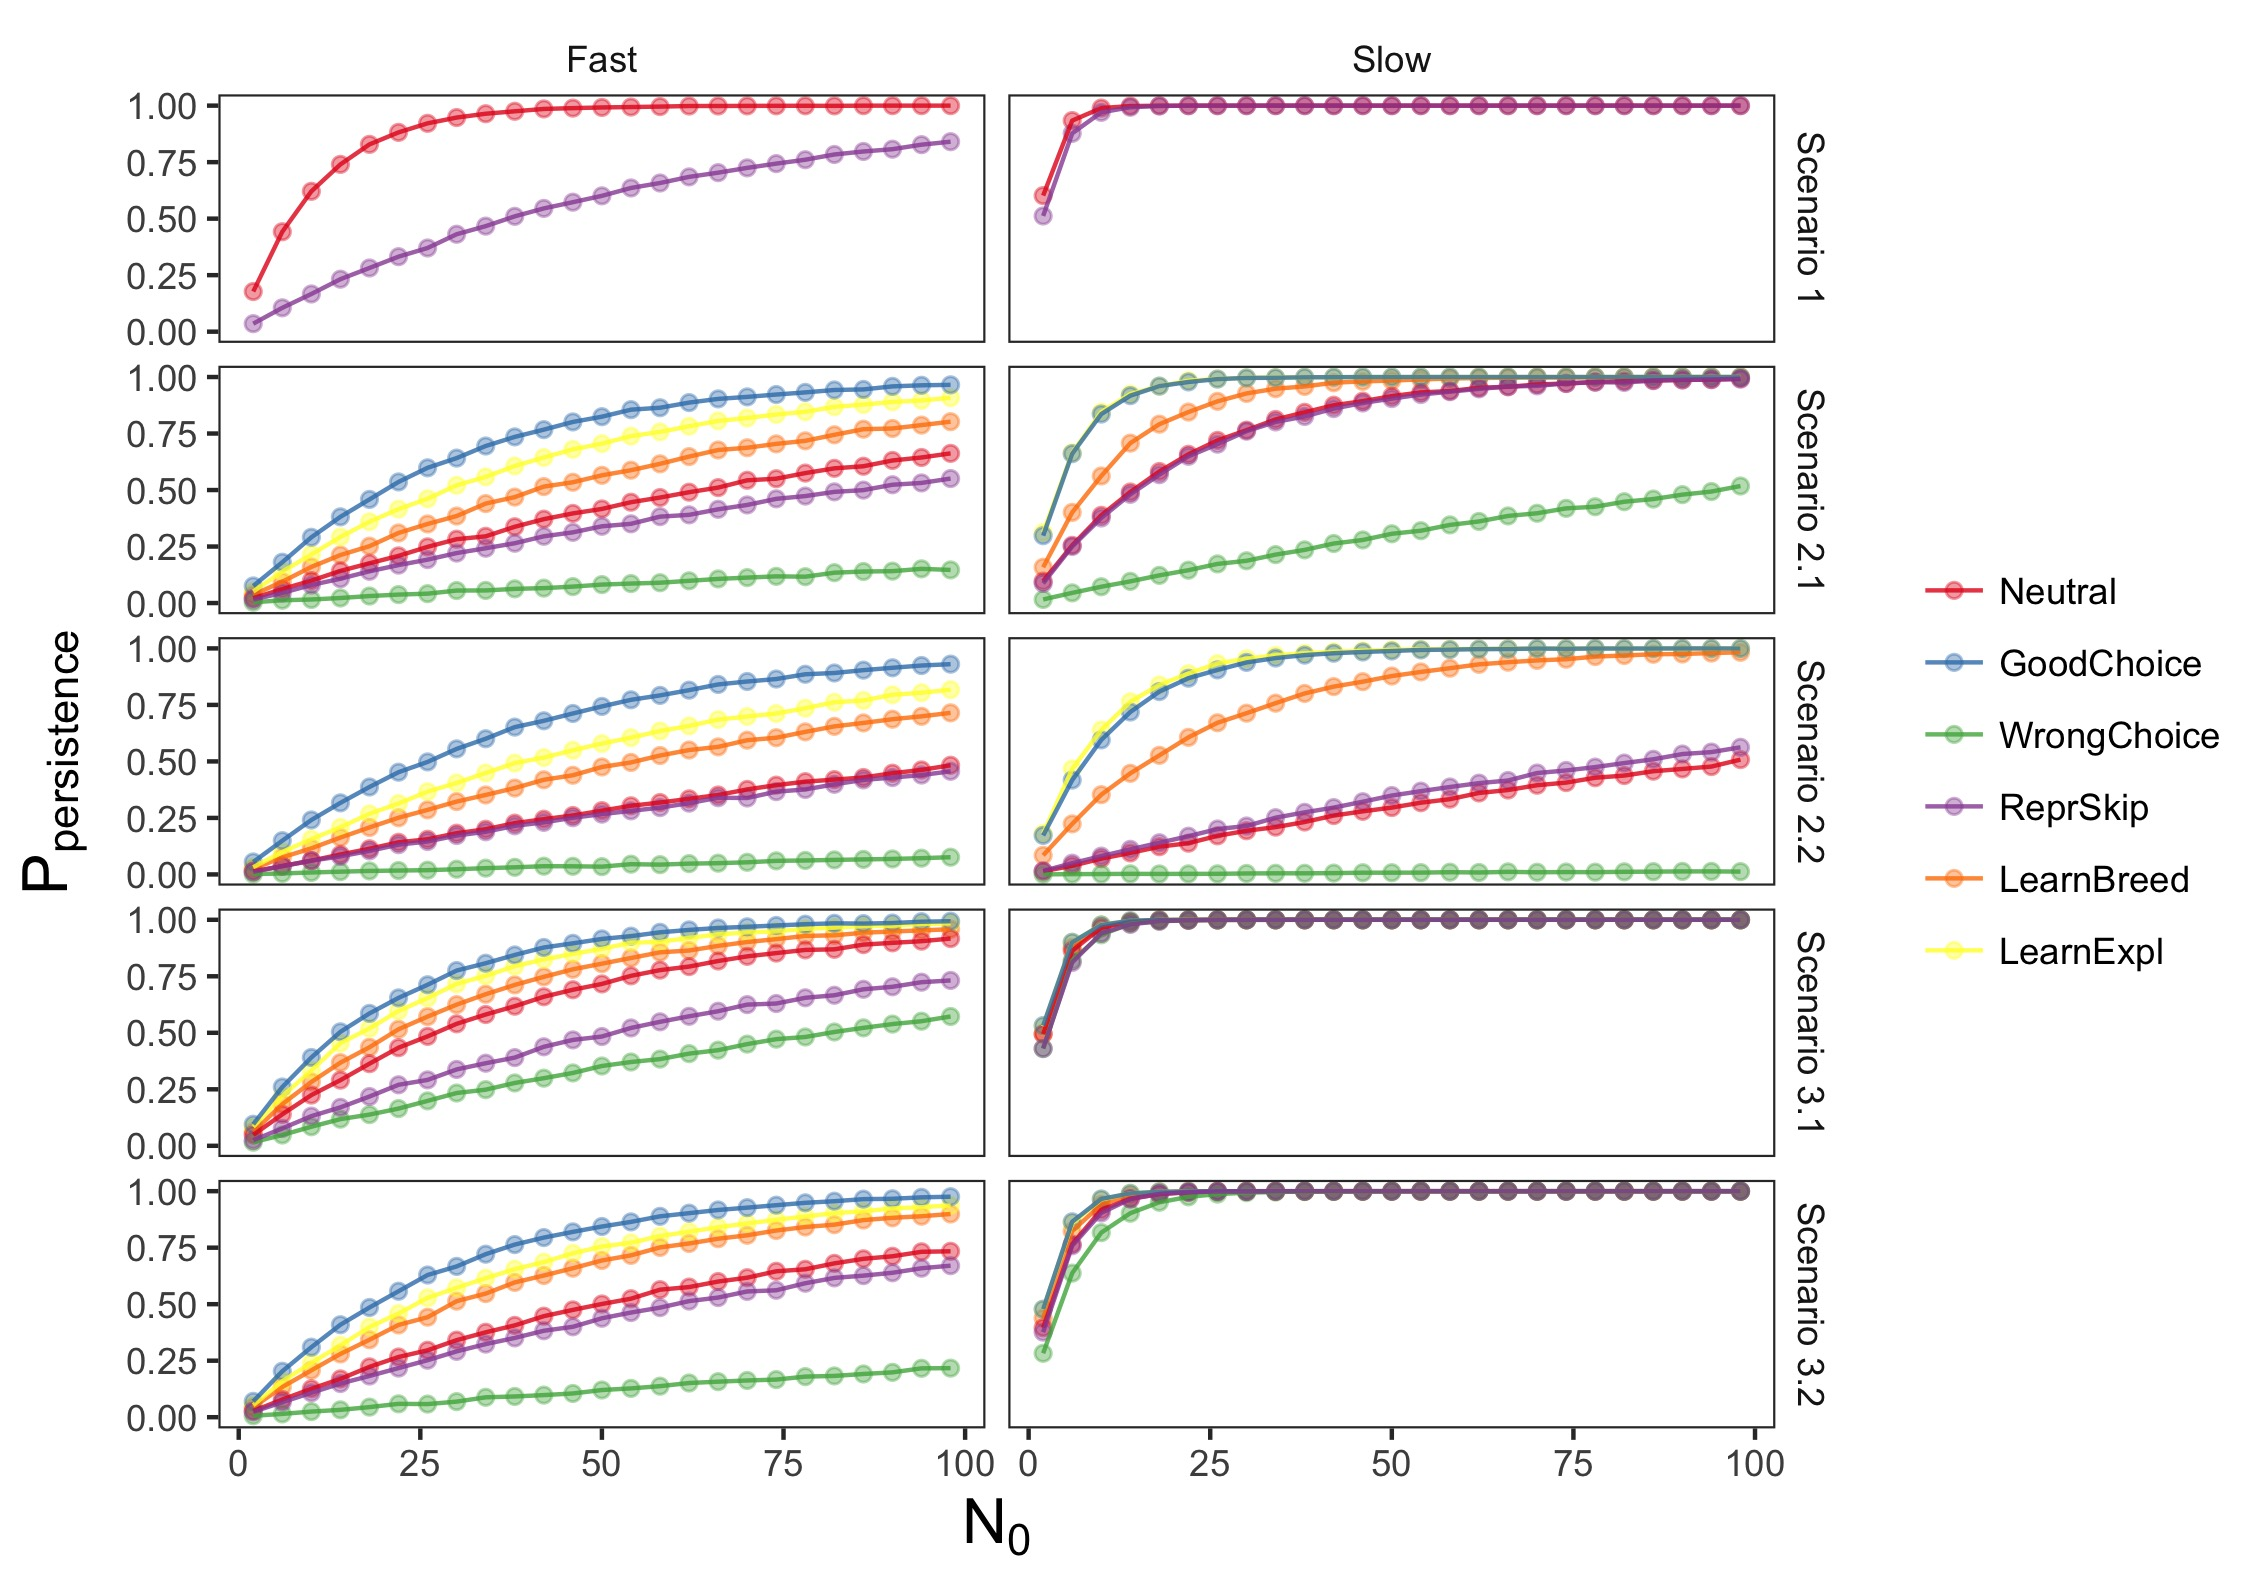
\includegraphics[width=\textwidth]{./Figures/chapter03/Fig_1.jpg}
\caption[Persistence as a function of LH, behviour and scenario]{
Simulations of probability of population persistence for 10 000 replicates as a
function of behavioural responses (\emph{Neutral}, random behavioural responses;
\emph{GoodChoice}, matching habitat choice; \emph{BadChoice}, habitat
mismatching choice; \emph{ReprSkip}, reproductive skipping; \emph{LearnExpl},
learning through exploration; \emph{LearnBreed}, learning from breeding
experience) for different initial population sizes according to different life
histories (fast and slow). Simulations have been run with the same deterministic
growth rate ($\lambda$) of 1.05 and moderate behavioural responses, under the
five different scenarios: phenotype – environmental matching (scenario 1) and
phenotype – environmental mismatch causing moderate increases of adult mortality
(scenario 2.1), extremely high adult mortality (scenario 2.2), moderate
increases of juvenile mortality (scenario 3.1) and extremely high juvenile
mortality (scenario 3.2). Simulations with strong behavioural responses are
shown in the electronic supplementary material, figure \ref{fig:figApp3.2.2}.
The fast strategy is characterized by early onset of first reproduction (1 year
old), high annual fecundity ($q = 8$) and low adult survival
($p_{1,s_{b}} = 0.4$), while the slow strategy exhibits delayed onset of
reproduction (3 years old), low fecundity ($q = 8$) and delayed onset of first
reproduction but high adult survival ($p_{1,s_{b}} = 0.85$). Note that in
scenario 1, the two habitats are the same, and therefore, all behavioural
responses except reproductive skip are equivalent to the neutral behaviour.}
\label{fig:fig3.1}
\end{figure}

We first illustrate the results of the model by presenting the
simulations for two species with the same maximum deterministic
growth rate ($\lambda = 1.05$) but striking differences in life
history, one being at the fast extreme of the fast–slow continuum
and the other at the slow extreme. Figure \ref{fig:fig3.1} presents
the simulated probability that these species thrive in a novel
environment as a function of initial population size ($N_{0}$),
according to different behavioural responses and scenarios of
maladaptation (see also the electronic supplementary material,
figure \ref{fig:figApp3.2.2}). In all the scenarios, the likelihood of establishment
increases with $N_{0}$ until reaching a threshold above which the
probability of population persistence is 1 (i.e. all simulated
populations become established). This pattern, which has
also been found empirically \citep{Blackburn2013, Sol2013}, reflects the pervasive
effect of demographic stochasticity at small population sizes.

In the absence of behavioural responses (red line), the curve
relating the probability of persistence and $N_{0}$ becomes flatter
under maladaptation (figure \ref{fig:fig3.1}, scenarios 2.1, 2.2, 3.1 and 3.2)
relative to scenarios where there is phenotype–environment
match. This is because the population not only suffers from
demographic stochasticity but also from the negative population
growth of the fraction of the population settled in the
low-quality habitat. The new route towards extinction largely
reduces population persistence, notably in scenarios where
the phenotype–environment mismatch is higher (electronic
supplementary material, figure \ref{fig:figApp3.2.2}, scenarios 2.2. and 3.2).

When individuals are allowed to take decisions, either
based on inherited or learned preferences, the probability of
persistence experiences substantial changes relative to the situation
where their behavioural responses are neutral (figure \ref{fig:fig3.1};
electronic supplementary material, figure \ref{fig:figApp3.2.2}). Matching
habitat choice and learning both contribute substantially to
increase the likelihood of persistence in a context of maladaptation.
Learning is generally not so efficient as an innate choice
based on perfect knowledge. When knowledge is imperfect,
however, innate responses can increase extinction risk by leading
individuals to choose an inappropriate habitat. Likewise,
the decision of skipping a reproductive event when conditions
are unfavourable often entails important fitness costs, reducing
the probability of establishment.


\subsection*{b) Integrating behavioural responses and life-history strategies}

\begin{figure}
\centering
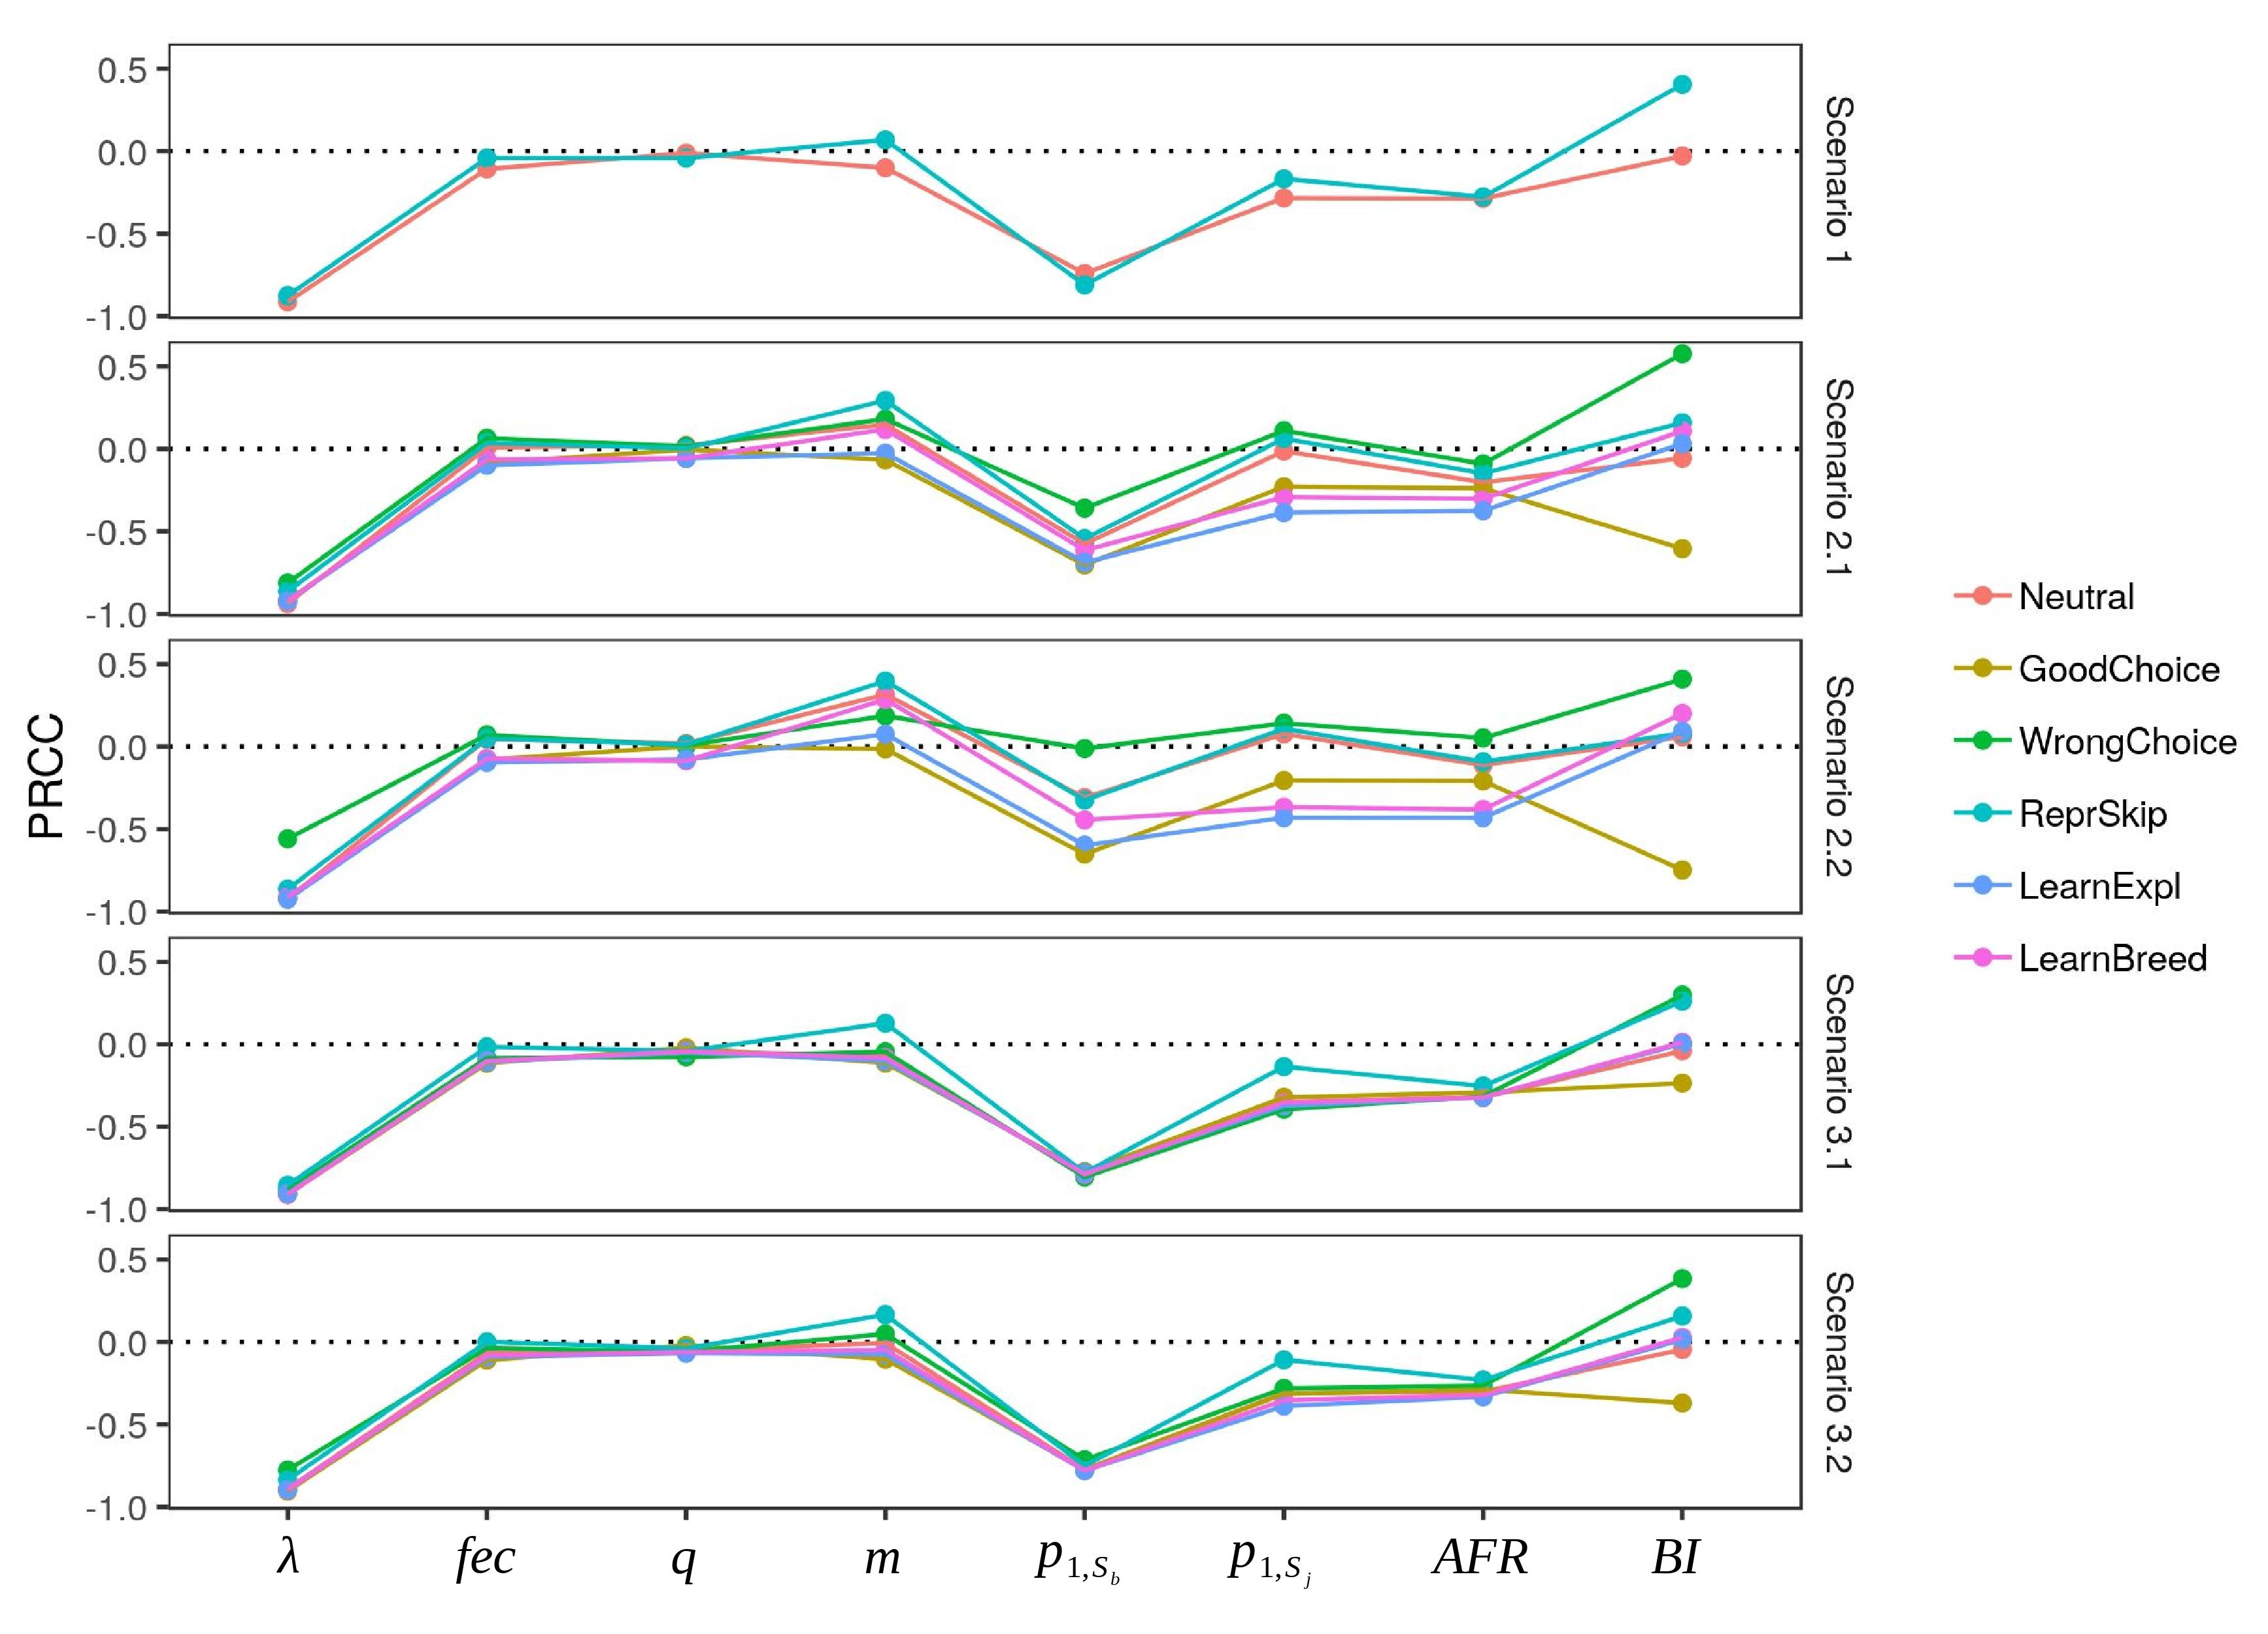
\includegraphics[width=\textwidth]{./Figures/chapter03/Fig_2.jpg}
\caption[Sensitivity of $N_{0}P_{50\%}$]{
Sensitivity of the probability of population persistence to life-history traits
for different behavioural responses and maladaptive scenarios, based on PRCC.
Population persistence is measured as $N_{0}P_{50\%}$, the initial population
that give a 50\% chance of persistence. Notation not shown in table
\ref{tab:table3.1} is as follows: $\lambda$ is the
deterministic grow rate; $fec$ is fecundity expressed as the number of offspring
produced annually ($m \cdot q$); $AFR$, is the age at first reproduction; $BI$
is the intensity of the behavioural responses, i.e. either moderate or strong.
Analyses are based on 3612 combinations of life-history traits distributing
species along the fast–slow continuum.}
\label{fig:fig3.2}
\end{figure}

Figure \ref{fig:fig3.1} suggests that the way behavioural responses influence
persistence in the novel environment differ according to the position
of the species in the fast–slow continuum. To formally
explore this, we repeated the simulations for the 3612 life-history
strategies resulting from all combinations of life-history
traits with $\lambda$ between 1.05 and 1.2 (see the section Exploration
of the parameters for details). For each life-history strategy,
we then estimated $N_{0}P_{50\%}$ to describe the likelihood that
the species persists in the novel scenario as a function of their behaviour.
Sensitive analyses across all scenarios and behavioural
strategies show that $\lambda$ is the most important factor facilitating
population persistence in the novel environments (figure \ref{fig:fig3.2}).
Life-history strategies with higher $\lambda$ show lower $N_{0}P_{50\%}$, implying
that they need fewer individuals to become established.
However, adult survival is the life-history trait with greater
influence in population persistence, suggesting that slow strategies
have generally higher chances than fast strategies to
persist in novel environments (figure \ref{fig:fig3.2}). The high persistence
of slow species in novel environments does not merely result
from the individuals initially introduced being able to survive
the entire simulation period. The explored life-history trait combinations
rarely allow individuals to survive 50 years, and in
most cases, the final population is higher than the initial one
(electronic supplementary material, figure \ref{fig:figApp3.2.3}).


\subsection*{c) Costs and benefits of behavioural responses in fast and slow strategies}

\begin{figure}
\centering
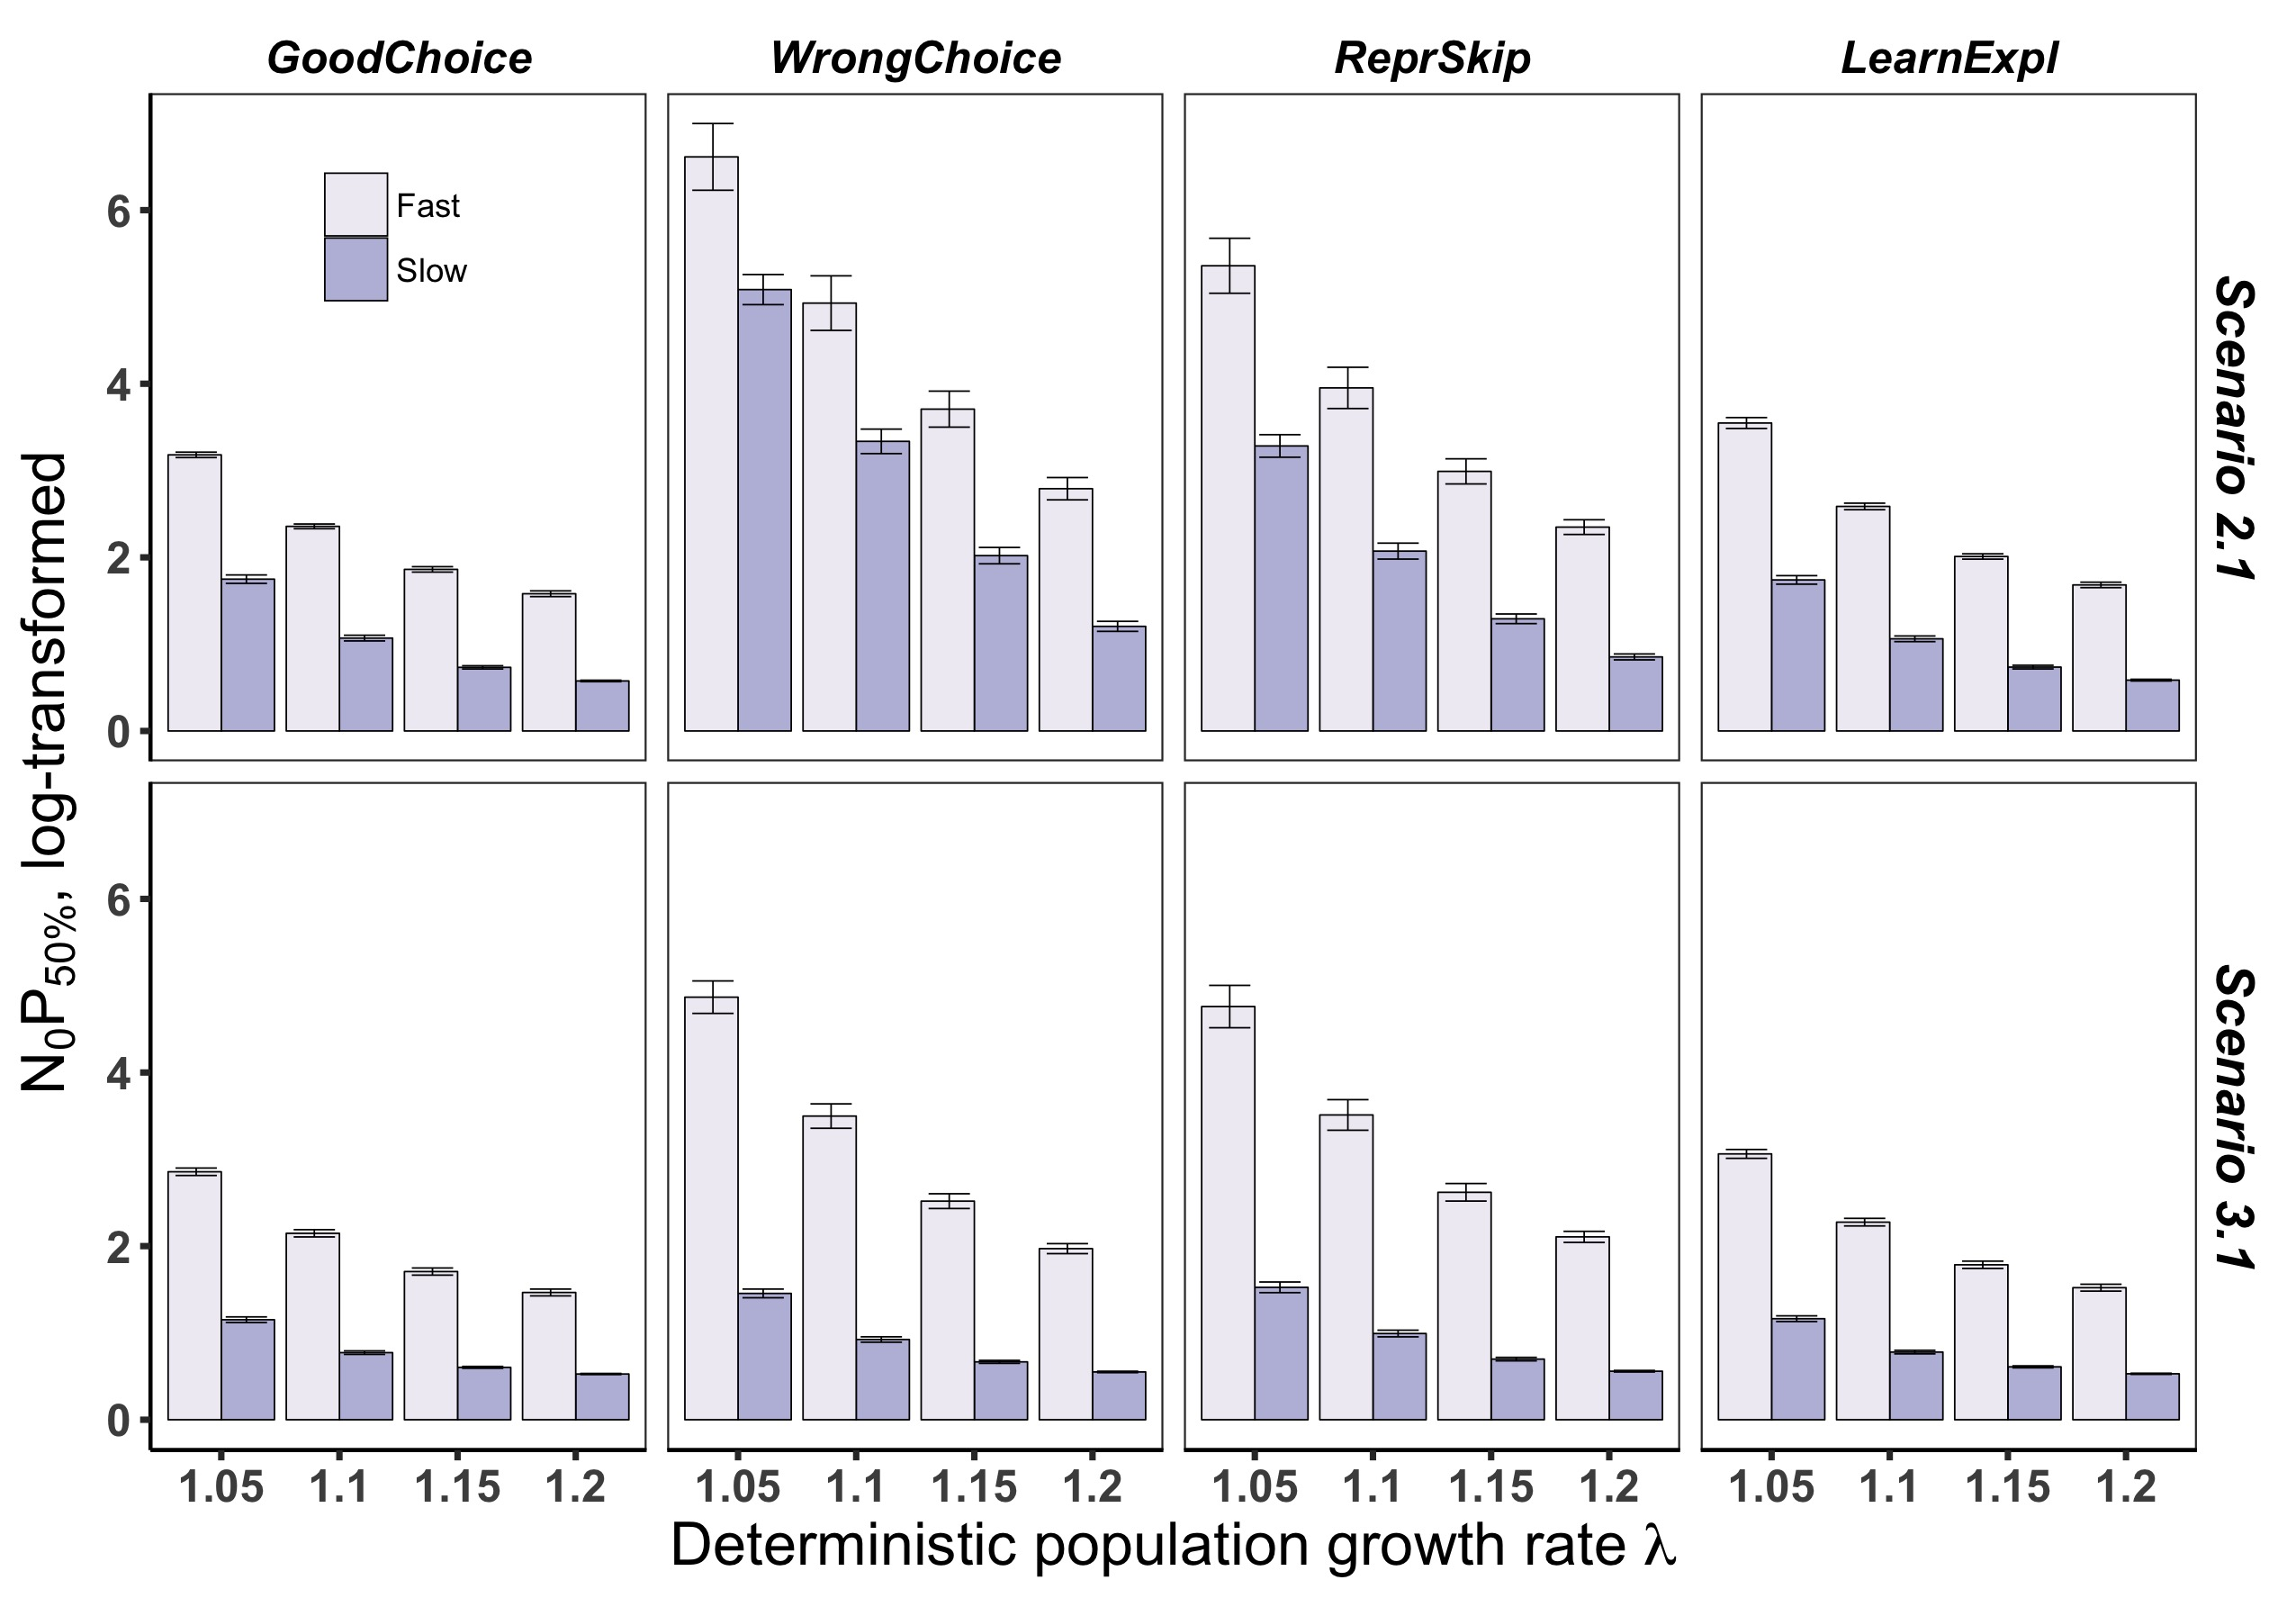
\includegraphics[width=\textwidth]{./Figures/chapter03/Fig_3.jpg}
\caption[Effects on $N_{0}P_{50\%}$]{
Effects of behavioural responses on population persistence in novel environments
as a function of the position of the animal along the fast–slow continuum.
Population persistence is estimated as $N_{0}P_{50\%}$ and behavioural responses
are moderate (for strong responses, see the electronic supplementary material,
figure \ref{fig:figApp3.2.4}). For details on abbreviations, see figure
\ref{fig:fig3.1}.}
\label{fig:fig3.3}
\end{figure}

To further investigate the interaction between behaviour and
life history, we compared life-history strategies positioned
either at the fast or slow extremes of the fast – slow continuum
(see the section Exploration of the parameters for details). The
results confirm that slow strategies generally need a lower
$N_{0}P_{50\%}$ than fast strategies to persist in the novel environments
(figure \ref{fig:fig3.3}). To reach a success similar to that of slow strategies,
fast strategies must have values of $\lambda$ substantially higher (often
more than 15\% higher) than those of slow strategies.

Under maladaptive scenarios, the probability of persistence
depends on whether the phenotype–environment mismatch
mainly affects offspring or adults, as fast and slow strategies
differ in their sensitivity to changes in fecundity and adult mortality.
Thus, although the general tendency of slow species to
be superior invaders is consistent across environmental scenarios,
slow species are particularly affected by scenarios
increasing adult mortality and fast species by those affecting
offspring mortality.

The benefits and costs of the behavioural responses are
also contingent to the position of the species along the fast –
slow continuum (figure \ref{fig:fig3.3}; electronic supplementary material,
figures \ref{fig:figApp3.2.6}–\ref{fig:figApp3.2.10}). In slow species, the gains of learning are substantial
when maladaptation increases adult mortality, while
the gains are almost negligible when maladaptation affects offspring
because they are already well protected for their life
history. Because slow strategies have more opportunities to
reproduce in the future, they are less penalized than fast
species by mistakenly choosing an inappropriate habitat to
reproduce. Likewise, the decision of skipping a reproductive
event when conditions are unfavourable, which is generally
costly (figure \ref{fig:fig3.1}), has a negligible impact on the demography
of slow species when the risk of reproductive failure is high.

For fast species, learning through exploration and an innate
preference for the high-quality habitat tend to improve population
persistence in all scenarios, although the gains are
modest and rapidly decrease at higher $\lambda$ values (figure \ref{fig:fig3.3}; electronic
supplementary material, figures \ref{fig:figApp3.2.6} and \ref{fig:figApp3.2.8}). Learning
from a reproductive failure is marginally beneficial only when
phenotype–environment match increases offspring survival,
even though the risk of extinction remains high (electronic
supplementary material, figure \ref{fig:figApp3.2.9}). The costs of preferring a
low-quality habitat or skipping a reproductive event are also
generally high in most scenarios, compared to those of slow
species, and generally cannot be compensated by increasing
$\lambda$ (electronic supplementary material, figure \ref{fig:figApp3.2.7}).


\section{Discussion}

Our results show strong support for the notion that behavioural
responses interact with life history to influence persistence in
novel environments. Under maladaptive scenarios, where the
match of the phenotype to the environment is insufficient,
the simulations suggest that it pays to have a slow life history
that increase the value of adults over the value of offspring
even at the cost of decreasing reproduction. This is in part
owing to the demographic consequences of the life-history
strategy itself and in part owing to the added benefits of behavioural
responses. Thus, a slow strategy represents a strong
buffer against maladaptation causing high offspring mortality,
indirectly affecting adult survival and hence the opportunities
for future reproduction. Instead, behavioural responses primarily
buffer individuals against maladaptation causing high
adult mortality. As novel environments are likely to increase
both adult and offspring survival, the complementary effects
of behavioural responses and life history make slow animals
particularly well equipped to cope with sudden changes in
the environment.

The notion that slow animals exposed to novel environments
generally gain greater benefits from behavioural responses has
been suggested in previous studies. Animals at the ‘slow’
extreme of the fast–slow continuum are generally believed to
explore more accurately the environment and exhibit better performance
in learning than those at the ‘fast’ extreme (reviewed in \citet{Sol2016}).
\citet{Eliassen2007}, for instance, developed a model to investigate
how foragers benefit from using a simple learning rule to
update estimates of temporal changes in resource levels; the
model showed that as lifetime expectancy decreases, learners
invest less in information acquisition and show lower foraging
performance when resource level changes through time. Our
simulations generally align with these studies, even though we
did not explicitly consider cognitive differences in learning
between fast and slow animals. Although it is likely that including
these differences accentuate the superiority of slow species in
contexts of maladaptation, this will depend on costs that are difficult
to estimate. Our model assumes some costs of behavioural
responses, such as imperfect information leading to choose a
low-quality habitat and a loss of breeding opportunities. However,
there are other costs not considered, such as those related
to the need to invest time and energy to produce and maintain
the neural and cognitive functions needed to acquire and
respond to environmental information.

A particularly intriguing question is to what extent innate
preferences and learning interact to influence the realized
preferences for habitats. \citet{Kawecki2010} argued that an individual
with no clear innate preference will be more amenable to
changing its preference as a result of experience than an individual
that already shows a strong innate preference, even
when it means choosing a low-quality resource. Thus, it
may be that some species primarily rely on matching the
environment to the phenotype through habitat matching
choice, while others rely more on improving the match of the
phenotype to the new environment through learning. Several
factors might contribute to favour one strategy over the other.
Natural selection on heritable variation in habitat preferences
should be more efficient in fast species, whose short generation
times increase mutation rates and changes in allele
frequency. Instead, in slow species that respond more
slowly to selection, learned preferences would outperform
genetically determined preferences (present study, see also \citet{Kokko2001}).
Learning might also be particularly favoured in ecological
generalists. A generalist strategy selects against local
adaptation \citep{Kisdi2002}, and frequently exposes individuals to new
challenges that require learned responses \citep{Sol2016a, Ducatez2015}. Our
simulations suggest an additional factor that might contribute to
favour learning over phenotype matching choice: the degree
of novelty in the environment. We find that learning does
not avoid extinctions as efficiently as perfect knowledge,
but in terms of population persistence, it avoids the risk of
falling into an ecological trap. Learning seems thus to be a
better strategy than matching habitat choice to thrive in
environments that are very different from the ancestral
environments or that change too fast to provide reliable
cues for habitat choice. One example could be urban environments.
These environments expose animals to a variety of
challenges that are drastically different from those found in
nature, such as the need to confront frequent disturbances
by people or avoid risks associated with traffic and buildings.
Growing evidence indicate that urban animals tend to be
more proficient in learning than non-urban animals \citep{Sol2013a}.

Our results contribute to the debate over whether successful
invaders should be characterized as fast or slow, an issue of
high relevance to predict and prevent the spread and impact of
biological invasions. Although life history has long been
deemed essential to understanding the success of invaders
\citep{Lewontin1969}, confidence in theoretical arguments has been undermined
by a perceived lack of empirical support \citep{Sol2012a}. The dissociation
between theoretical and empirical work has in part been attributed
to the excessive focus on the ‘small population paradigm’
\citep{Sol2016}, which assumes that demographic stochasticity is the main
driver of extinction in introduced populations. This has led to
the widespread belief that successful invaders are characterized
by high fecundity that reduces the risk of stochastic
extinctions by facilitating rapid population growth from
small initial populations. While this process has received
some empirical support \citep{Allen2017, Capellini2015}, our results align with theoretical
and empirical work suggesting that it mainly applies when
the organism’s phenotype matches well with the environment
\citep{Sol2012a, Jeppsson2012}. Yet, under maladaptive scenarios our simulations
indicate that fast strategies are more affected by ecological traps
and are only superior to slow strategies when their population
growth rate is substantially higher. Moreover, this superiority
is only noticeable when the phenotype mismatch with the
environment increases adult mortality, reflecting that population
growth of fast species is less sensitive to changes in
adult mortality than in fecundity. Given the importance of parental
care in many animals, however, it is unrealistic to assume
that a high adult mortality will not be accompanied by
increased offspring mortality \citep{Santema2018}. The crucial question is
therefore to what extent fast animals can maintain high population
growth rates in a context of maladaptation. Current evidence
in birds and mammals does not indicate that fast species
have higher population growth rates in the wild than slow-lived
species (electronic supplementary material, figure \ref{fig:figApp3.2.11}).
To properly clarify this issue on empirical grounds, however,
we would need field estimations of population growth rate
for fast and slow populations exposed to different degrees of
phenotype–environment mismatch. Unfortunately, this type
of information is currently unavailable.

As any model, ours is a simplified representation of the reality.
An issue that remains insufficiently resolved is how different
behavioural responses affect establishment success when acting
in concert. In our simulations, we have investigated behavioural
mechanisms separately, to be able to disentangle their effects, but
in reality, it is likely that they act in concert, either synergically or
antagonistically. The challenge here is to parametrize the models
in a way that is realistic enough to avoid biasing the simulations,
but this requires a better understanding of mechanisms. Another
issue that will need further attention in the future is the possibility
that other mechanisms in addition of those analysed here
also influence the response to environmental changes. We have
previously suggested that producing several broods in the
same breeding season can afford high benefits when the chances
of a reproductive failure are high, as it provides the advantage of
a high annual fecundity while reducing the costs of a reproductive
failure \citep{Sol2012a}. Future models will also have to consider Allee
effects, that is, the decline in the rates of reproduction and/or survival
at low population densities. These effects are not only
highly relevant during the early stages of the invasion process,
but may also be tied to the life history and behavioural strategies
of the species \citep{Leung2004}. A preference for a low-quality habitat is
indeed a type of Allee effect, as it slows population growth at
low densities \citep{Kokko2001}, but other types of Allee effects could also be relevant
\citep{Reznick2002}. Allee effects are expected to be particularly relevant in
highly social animals that rely more on social and public information
to take decisions and learn. Advancing in all these
themes will offer a more complete picture of how animals cope
with environmental changes.

Although organisms that are slow-lived relative to the rate
of environmental fluctuations often exhibit enhanced learning
abilities \citep{Sol2016a}, the evolutionary causes are less well understood.
It has been suggested that the causal link between learning and
longevity could be bi-directional \citep{Eliassen2007, Ratikainen2019, Sol2009a}. The possibility of
constructing behavioural responses to ecological challenges
might directly affect the evolution of life histories by buffering
individuals from extrinsic mortality. The evolved combination
of life-history traits might in turn alter the fitness benefits and
costs of behavioural responses, as suggested here. However,
the covariation between learning and life history can also
result from correlated evolution \citep{Sol2016a}. Our results reinforce
this latter view, suggesting that the environments which
favour slow life-history strategies are similar to those favouring
learning. Thus, behavioural plasticity and slow life histories
might be dimensions of a same pace-of-life syndrome to cope
with sudden environmental changes \citep{Sol2016a}.

We have shown that considering variation in life-history
species is relevant when predicting the influence of behaviour
on the probability of persisting in novel environments.
Although the interplay between behaviour and life history
is still insufficiently understood, our results highlight that
to continue advancing, we need to acknowledge that both
may be part of a broader adaptive system of organisms to
cope with rapid environmental changes.

%************************************************
\chapter[Risk-taking behavior, urbanization and POLS]{Risk-taking behavior,
urbanization and the pace of life in birds
  \footnote{Published in: Sol, D., J. Maspons, A. Gonzalez-Voyer, I. Morales-Castilla, L. Z.
  Garamszegi, A. P. M\o{}ller. 2016 Risk-taking behavior, urbanization and the
  pace of life in birds. \textit{Behav. Ecol. Sociobiol}. 72, 59.
  \href{http://dx.doi.org/10.1007/s00265-018-2463-0}{doi:10.1007/s00265-018-2463-0}
  }
}\label{ch:POLS}
%************************************************


\section*{Abstract}

Despite growing appreciation of the importance of considering a pace-of-life syndrome (POLS) perspective to understand how
animals interact with their environment, studies relating behavior to life history under altered environmental conditions are still
rare. By means of a comparative analysis of flight initiation distances (i.e., the distance at which an animal takes flight when a
human being is approaching) across \textgreater{300} bird species distributed worldwide, we document here the existence of a POLS
predicted by theory where slow-lived species tend to be more risk-averse than fast-lived species. This syndrome largely emerges
from the influence of body mass, and is highly dependent on the environmental context. Accordingly, the POLS structure
vanishes in urbanized environments due to slow-lived species adjusting their flight distances based on the perception of risk.
While it is unclear whether changes in POLS reflect plastic and/or evolutionary adjustments, our findings highlight the need to
integrate behavior into life history theory to fully understand how animals tolerate human-induced environmental changes.


\section*{Significance statement}

Animals can often respond to changing environmental conditions by adjusting their behavior. However, the degree to which
different species can modify their behavior depends on their life history strategy and on the environmental context. 
Species-specific perception of risk is a conspicuous example of adjustable behavior tightly associated with life history strategy. While
there is a general tendency of higher risk aversion in rural than city-dwelling birds, it is dependent on the species’ life history
strategy. Slow-lived species are more prone to adjust their flight initiation distances based on the perception of risk, allowing
humans to approach closer in urban than rural environments. Behavior must therefore be taken into account together with life
history to reliably assess species’ vulnerability at the face of ongoing environmental change.

\bigskip
\textbf{Keywords:} Life history theory, Phenotypic plasticity, Human-induced rapid
environmental changes, Learning

\clearpage


\section{Introduction}

Behavior is widely considered one of the main mechanisms
through which animals cope with changes in the environment
\citep{Bogert1949, Klopfer1962, mayr1965}. Unlike other phenotypic
features, behavior can often be rapidly modified to solve
new ecological problems, thus contributing to reduce the uncertainties
and adaptive mismatches that arise when environmental 
conditions change \citep{Huey2003, Price2003, Estrada2016, Sol2016}. 
A growing number
of studies has for instance documented that animals living
in urban environments differ in behaviors related to resource
use, disturbance avoidance, and communication from those
inhabiting little urbanized environments (reviewed in 
\citet{Shochat2006, Evans2012, Lowry2013, Sol2013a}). 
Evidence is also accumulating that these behavioral differences
primarily reflect plastic adjustments, although some
may also result either from selection or from a non-random
sorting of individuals by behaviors that affect colonization success
(reviewed in \citet{Sol2013a}).

Despite the plastic nature of most behaviors, some animals
exhibit strong consistencies in how they behave across time
and contexts (reviewed in \citet{Sih2004, Reale2007}).
These behavioral consistencies are expressed among individuals
within species, as well as among individuals of distinct
species (e.g., \citet{Moller1994, Verbeek1994, Koolhaas1999, Gosling2001, Greenberg2003, Sih2004, Reale2007}).
An example is a behavioral syndrome where
some animals are risk-averse whereas others are risk-prone
across a range of situations regardless the actual risks \citep{Sih2004, Sih2012a}.
This syndrome has attracted considerable
interest of behavioral ecologists because the inability of individuals
to adjust their behavior to the actual level of risk can
entail important costs, such as greater exposure to predators,
reduced foraging opportunities and increased energetic expenditure
\citep{Sih2004, Sih2012a}. However, the reasons why some
animals readily adjust their behavior in response to novel situations
while others persist with their behavior, even when maladaptive,
remains unresolved \citep{Sih2004}. Recently, it has
been suggested that the striking consistencies in risk-taking
behavior observed across individuals of a given species, but
not in members of other species, can be understood if we consider
behavior and life history as dimensions of a same pace-of-life
syndrome (POLS) \citep{Wolf2007, Reale2010a}.

The POLS theory argues that animals experiencing different
environmental conditions should diverge in a suite of behavioral
and physiological traits according to their life history 
\citep{Ricklefs2002, Tieleman2005, Hau2010a, Reale2010a}. 
A central premise of this theory is the existence of a
fast-slow continuum of life history variation (FS hereafter),
which reflects the impossibility to simultaneously maximize survival
and fecundity \citep{Stearns1983a, Saether1988}. The FS aligns
organisms along a pace-of-life (POL) axis from a ``highly
reproductive'' (fast-lived) strategy at one end to a ``survival''
(slow-lived) strategy at the other end. As slow-lived animals
prioritize future over current reproduction \citep{Stearns2000}, they
should generally be more risk-averse compared to those at the
fast extreme \citep{Martin2000, Wolf2007, Hau2010a, Moller2012, Moller2013a}.
In contrast, fast-lived animals should prioritize behaviors that
enhance current reproductive effort, even when doing so involves
taking some risks. Therefore, the POLS theory explicitly verbalizes
the classic idea that selection should favor behaviors ensuring
higher adult survival in slow-lived animals and behaviors that
enhance reproductive effort in fast-lived animals.

Despite the existence of theoretical predictions, empirical
support for the existence of a risk-taking POLS is currently
scarce \citep{Hille2015, Charmantier2017}. A %Wrong year for Hille 2014 in the original article
number of factors may indeed prevent the detection of such a
POLS. One is the extent to which risk-taking behaviors can be
modified by learning. Slow-lived species have less cognitive
and time constrains to gather new environmental information
and accommodate their behavior accordingly by means of
learning \citep{VanSchaik2003, Sol2009a, Sih2012, Sol2016a}.
If plastically modifying FID
depends on the position of the animal in the fast-slow continuum,
the POLS may vanish in contexts where the perception
of risk is low.

Another factor that makes the demonstration of POLS challenging
is the low heritability of life history traits \citep{Price1991}.
The analysis of individual variation within
populations is fundamental to disentangle the importance of
plasticity and genetic processes, as well as being of interest in
itself \citep{Reale2007}. However, the low heritability of life
history traits reduces the likelihood of detecting POLS at the
individual level. An obvious alternative is to examine POLS
across populations or species, as they have had more opportunities
to diverge in behavioral and life history traits, yet such
a level of analysis is more rarely used.

Here, we investigate if risk-taking behaviors are a defining
part of a POLS syndrome in birds, and ask to what extent the
syndrome can be relaxed according to the environmental conditions.
We focus on behavioral and life history differences
across species exposed to contrasting degrees of human disturbances.
Our measure of risk-taking behavior is the flight
initiation distance (FID), defined as the distance at which an
individual takes flight when approached by a human. Previous
work in birds has shown that FID within and across species is
shorter in urbanized than in non-urbanized environments
\citep{Moller2008, Carrete2011, Sol2012b},
indicating that the perception of risk is context-dependent. We
take advantage of these previous findings to address two main
expectations of POLS theory regarding risk-taking behavior.
The first is the expectation that slow-lived species should exhibit
longer FID than fast-lived species when the perception of
risk is high. Although FID has been found to be positively
related to certain vital rates in birds, like fecundity \citep{Blumstein2006, Moller2012}, 
the fast-slow continuum
is better characterized in the context of the full life cycle of a
species \citep{Adler2014}. We operationally defined the continuum
as the combination of life history traits that better
predicts the fecundity-survival trade-off \citep{Caswell2000, Oli2003, Oli2004}. 
We then used information on
\textgreater{11,000} measures of FID belonging to \textgreater{300} avian species to
ask whether flight distances vary depending on the position of
the species in the fast-slow continuum. To this purpose, we
used phylogenetic Bayesian mixed models that allow the integration
of species-level information generated by observations
of multiple individuals. As theoretical and empirical evidence
suggests that both the fast-slow continuum \citep{stearns1992evolution} 
and FID \citep{Moller2015} are positively correlated with
body size, we also examined whether body size may be one of
the factors underlying the FID-FS association.

The second expectation of POLS theory is that slow-lived
species can better accommodate their FID to the perception of
risk than fast-lived species. This expectation derives from the
supposed higher behavioral plasticity of slow-lived species
\citep{Sol2009}, which would allow them to habituate faster to
human presence, and from constraints in fast-lived species to
adopt risk-averse strategies due to the need to prioritize reproduction.
We validated this prediction by investigating how
FIDs change between urban and rural habitats as a function
of the position of the species in the fast-slow continuum, again
using phylogenetic Bayesian mixed models. Following suggestions
that behavioral differences between urban and non-urban
birds might be linked to brain size and learning capabilities
\citep{Kark2007, Maklakov2011, Sol2011}, 
we also verified whether a larger brain size contributes
to explain why slow-lived species should be better able to
accommodate FID to risk perception \citep{Sol2009a, Sol2009}.


\section{Material and methods}

\subsection*{Measuring FID}

A total of 11,863 FID observations were recorded by one of
the authors (APM) during February–September 2006–2014,
using a standard experimental field procedure \citep{Hediger1934, hemmingsen1951relation, Blumstein2006}. 
All estimates were collected
blindly with respect to the hypotheses being tested here,
thereby preventing any conscious or unconscious bias. The
observations were made in an area of 100 km2 in Orsay (48°
42’ N, 2° 11′ E, France), 800 km2 in Northern Jutland (57° 12’
N, 10° 00′ E, Denmark), 500 km2 in Oslo (59° 54’ N, 10° 45′
E, Norway), and 500 km2 on Hainan Island (19° 12’ N, 109°
42′ E, Southern China). In most regions, observations were
carried out in both urban habitats (i.e., areas with multistory
buildings, single-family houses, roads, and urban parks) and
rural habitats (i.e., open farmland and woodland lacking continuous
urbanized areas). Therefore, our distinction between
urban and rural habitats essentially separates environments
very frequented by humans from those less frequented.

To record FIDs, the observer located an individual bird
with binoculars and subsequently moved at a normal walking
speed towards the individual, while counting the number of
steps (which approximately equals the number of meters
\citep{Moller2008}). The FID was the horizontal distance at which
the individual took flight. The starting distance (i.e., the distance
from where the observer started walking up to the bird)
was in most cases (\textgreater{98\%} of all observations) fixed at ca. 30 m
to avoid confounding FID with starting distance. If the bird
was located in the vegetation, the height above ground was
also recorded to the nearest meter using the observer as a
yardstick. This method is reliable when cross-validated using
a laser Bushnell® Elite 1500. FID was then estimated as the
Euclidean distance, which equals the square-root of the sum of
the squared horizontal distance and the squared height above
ground level \citep{Blumstein2006}. When possible, sex (n = 4958
observations), age (n = 10,887), and flock size (n = 1387)
were also recorded to be included as confounds in the models.
Although the FID of some individuals was measured twice,
we only used the first measure in the analyses. All FID data
are available as supplementary material.


\subsection*{Measuring POL}

To estimate the fast-slow continuum, we searched for published
information on six life history traits: (1) clutch size,
(2) number of broods per year, (3) maximum lifespan (years),
(4) incubation period (days), (5) nestling period (days), and
(6) age at first reproduction (years). We found information of
all six traits for 765 avian species (see \citet{Sol2016a}). As
originally defined, the fast-slow continuum results from the
existence of a fecundity-survival trade-off \citep{stearns1992evolution}.
Consequently, we empirically defined the fast-slow continuum
as the combination of life history traits that better predicts
the relative sensitivity (i.e., elasticity) of population growth to
changes in adult survival \citep{Caswell2000, Oli2003, Oli2004}. 
To this purpose, we used the COMADRE
Matrix database \citep{Salguero-Gomez2016} to obtain 
age-structured population matrices that incorporate accurate information
on the rates of survival, growth, and reproduction from
natural populations. We removed four matrices for which elasticities
did not sum up to 1, which could reflect mistakes in the
data, and for the remaining matrices (n = 53 from 49 species),
we estimated the elasticity for adult survival. To combine the
life history traits, we conducted phylogenetic principal
component analyses (PPCA) \citep{Revell2009a} based on the 765
species, including a minimum of three traits in each analysis
(i.e., 42 PPCAs). The species scores of each PPCA was then
used as predictor of elasticities in a phylogenetic least square
models (PGLS) \citep{Orme2013}, and the best models were
classified according to AICc. The combination of life history
traits that best predicted variation in elasticity for adult survival
included lifespan, clutch size, and fledging period. We
therefore defined the position of each species in the fast-slow
continuum by extracting the scores of this PPCA. In
our best PPCA, species with high scores (i.e., high adult survival
elasticities) were slow-lived and those with low scores
(i.e., high fecundity elasticities) were fast-lived. We note that
the results of our approach based on adult survival elasticities
are similar to those based on estimates of elasticities for fecundity
or on generation time extracted from the demographic
matrices (see Chapter \ref{ch:LHaxes}).


\subsection*{Modeling FID}

To model variation in FID, we used Bayesian phylogenetic
mixed models (BPMM) with Gaussian error structure, as im-
plemented in the R package ``MCMCglmm'' \citep{Hadfield2010, Hadfield2010a}. 
FID was log transformed before
analyses to improve model convergence. As our units of
analysis were the FID observations, species identity was included
as a random factor together with phylogeny. The phylogeny
was a maximum clade credibility phylogeny (CCP)
consensus tree based on a sample of 1000 phylogenies from
the pseudo-posterior distribution in \citet{Jetz2012}, built with
the TREEANNOTATOR software \citep{Drummond2012}.
When appropriate, country was also included as a random factor
to better account for data heterogeneity (see results for details).
We first ran models without predictors to estimate FID
consistency within species and phylogenetic heritability by
means of a variance components analysis \citep{Housworth2004}. 
Then, we added predictors as fixed effects to explain
variation in FID. To demonstrate the existence of POLS, we
modeled FID as a function of the fast-slow continuum, including
habitat (i.e., rural or urban), sex, age, flock size, and height
at which the bird was observed as possible confounding effects.
Using non-informative priors, the MCMC chains were run for
330,000 iterations with a burn-in interval of 30,000 and sampling
each 300 iterations to ensure satisfactory convergence.

As we found evidence for a link between FID and FS, we
tested whether this was caused by their common association
with body size. To this purpose, we used phylogenetic path
analyses on species’ trait averages \citep{VonHardenberg2013, Gonzalez-Voyer2014}. 
The minimal set of conditional independencies for each
path model \citep{VonHardenberg2013} was
tested using PGLSs models as implemented in the package ape
\citep{Paradis2004} in R. Models were run estimating an evolutionary
parameter ($\lambda$) simultaneously with model fit that adjusts
the variance–covariance matrix to adequately fit the model
of evolution, in our case a Brownian motion model \citep{Freckleton2002}. 
The fit of a given path model to the data was
estimated via the C statistic. The C statistic tests whether the
minimum set of conditional independencies of a model is fulfilled
by the observational data, thus it provides an estimate of
the goodness of fit of the model to the data \citep{Shipley2013}. A
significant C statistic indicates that the model is a poor fit to the
data. We employed an information theoretical approach and
compared the different path models using the C statistic information
criterion (CICc; analogous to the Akaike information
criterion; \citet{VonHardenberg2013}).

We finally investigated whether changes in FID between
urban and rural habitat were larger in slow-lived species than
in fast-lived species, using the same BPMM approach described
above. To do so, we averaged the FID values of each
species per habitat and then estimated FID difference as
$$log(mean FID_{rural}) - log(mean FID_{urban})$$
We therefore only
used species present in both habitats for the analyses. FID
differences were then used as response variable in a BPMM
with the fast-slow continuum as fixed effect and the phylogeny
as a random factor. Unlike previous models, the level of
analysis here was the species instead of FID observations.
Thus, the conclusions could be sensitive to the sample size
used to estimate FID differences. We tackled this limitation in
two ways. First, in the BPMM we weighted FID differences
by 1/(n−3), being n the number of individuals sampled per
species. Second, we re-ran the model for the subset of species
with at least 15 FID observations in each habitat. To test
whether differences in FID across habitats were related to
differences in brain size, we used information published in
\citet{Sayol2016} on the residuals of a log-log PGLS of brain
volume against body mass. Positive residuals mean that the
brain of the species is larger than expected by body size and
negative residuals that is smaller than expected by body size.


\section{Results}

\begin{figure}
\centering
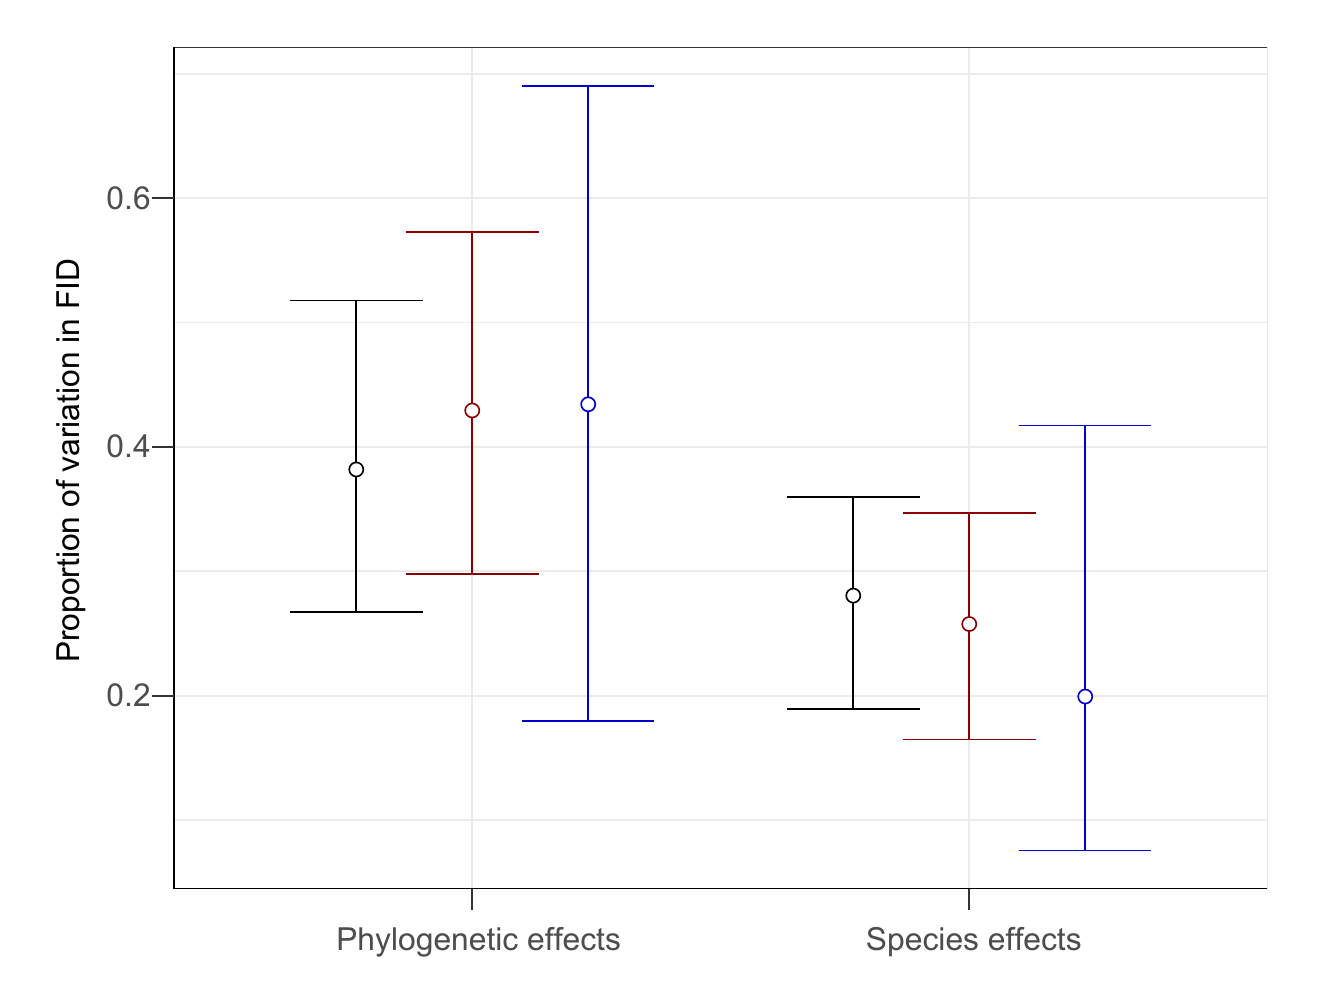
\includegraphics[width=0.75\textwidth]{./Figures/chapter04/Fig_1.png}
\caption[Variance in FID accounted for the phylogeny and species]{
Proportion of variance in FID accounted for the phylogeny and
within species variation when considering all observations (black), rural
observations only (red) and urban observations only (blue). Values are the
intra-class coefficients estimated by means of a BPMM with the constant
as fixed effect and the phylogeny and species identity as random factors.
Error bars are 95\% credible intervals.}\label{fig:fig4.1}
\end{figure}

A Bayesian phylogenetic mixed model (BPMM) based on 11,852
observations of 317 bird species confirmed the existence of consistent
among-species variation in FID (mode = 0.65, CI = 0.57–
0.77), much of which was shared among close relatives (Fig. \ref{fig:fig4.1},
Table \ref{tab:tabApp4.1}). FID did not vary with sex (pMCMC = 0.920), age
(pMCMC = 0.518), and flock size (pMCMC = 0.696). However,
birds did tend to exhibit longer FID when located at certain height
above the ground (mode = 0.026, CI = 0.013–0.038). Of the remaining
residual variation, a significant fraction was accounted for
differences among habitats. As shown in previous studies
(reviewed in \citet{Moller2014a}), FID was consistently shorter in urban
than in rural habitats across all study regions (pMCMC \textless{0.0001},
Fig. \ref{fig:fig4.2}, Table \ref{tab:tabApp4.2}). Variation in FID across species was also more
consistent in rural than in urban habitats (Fig. \ref{fig:fig4.1}).

\begin{figure}
\centering
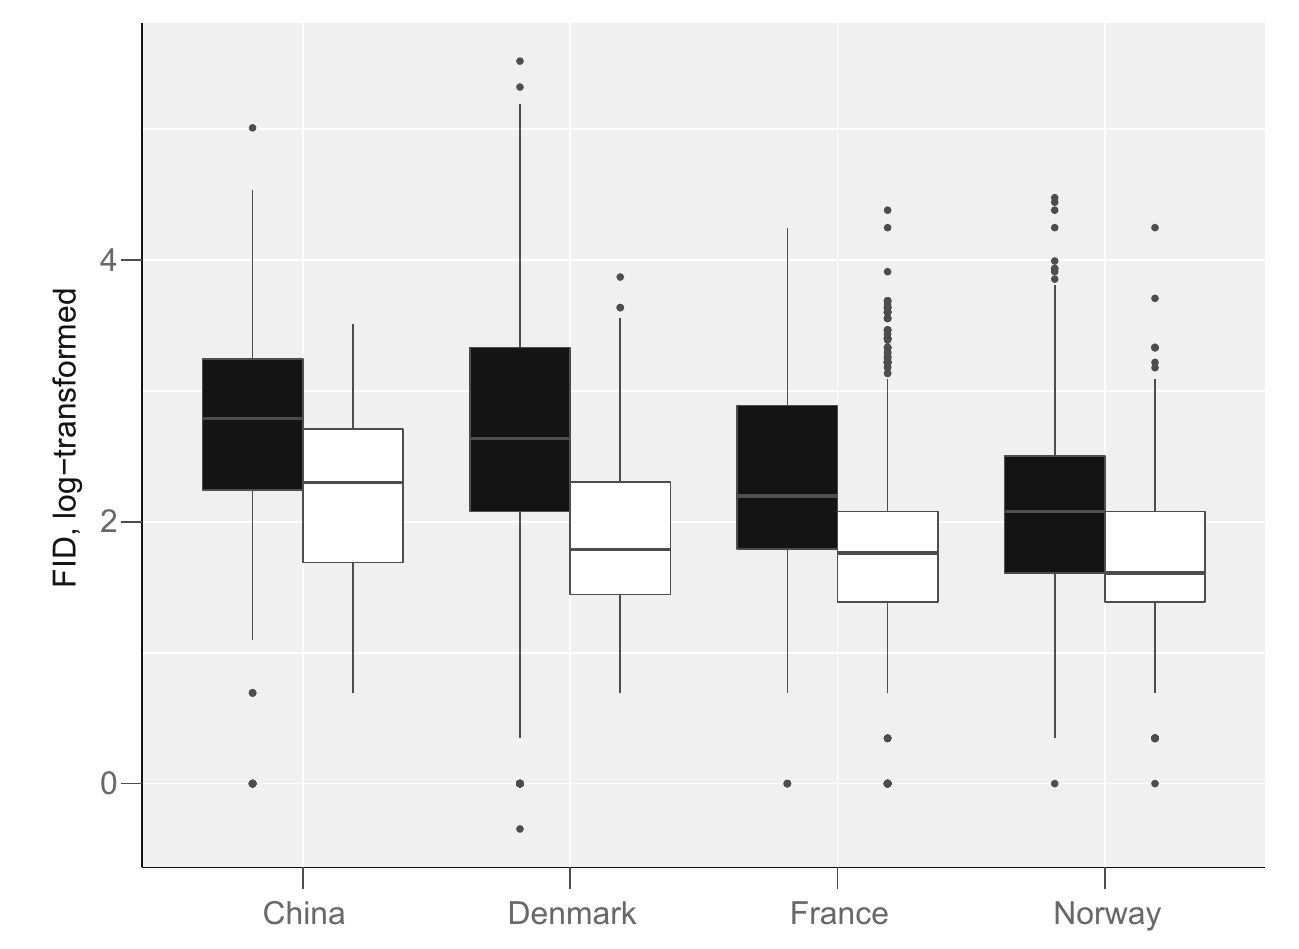
\includegraphics[width=0.75\textwidth]{./Figures/chapter04/Fig_2.png}
\caption[FID across countries]{Differences in FID between urban (white) and rural
(black) habitats across countries. The plot shows the median,
interquantile range and 1st and 3rd quartiles.}\label{fig:fig4.2}
\end{figure}

The studied species exhibited substantial variation in their
position along the fast-slow continuum, reflecting the existence
of a fecundity-survival trade-off (Fig. \ref{fig:fig4.3}). As expected, species at
the slow extreme of the continuum tended to exhibit longer FID
than those at the fast extreme (pMCMC \textless{0.0001}, Table \ref{tab:tabApp4.3}),
consistent with the existence of a POLS. However, there was a
negative interaction with habitat (Table \ref{tab:table4.1}), reflecting that FID
and life history variation became decoupled in urban environments
(Fig. \ref{fig:fig4.4}). This pattern was largely due to changes in FID
across habitats by slow-lived species (Table \ref{tab:table4.2}, Fig. \ref{fig:fig4.4}). In rural
environments, where the POLS was detected, the best phylogenetic
path models suggest that the FID-FS association was primarily
caused by their common association with body size
(Figs. \ref{fig:fig4.5}, \ref{fig:figApp4.2}). In urban environments, there is no direct effect of
body size on FID, which might explain why the FID-FS association 
is no longer present (Figs. \ref{fig:fig4.5}, \ref{fig:figApp4.3}).

\begin{figure}
\centering
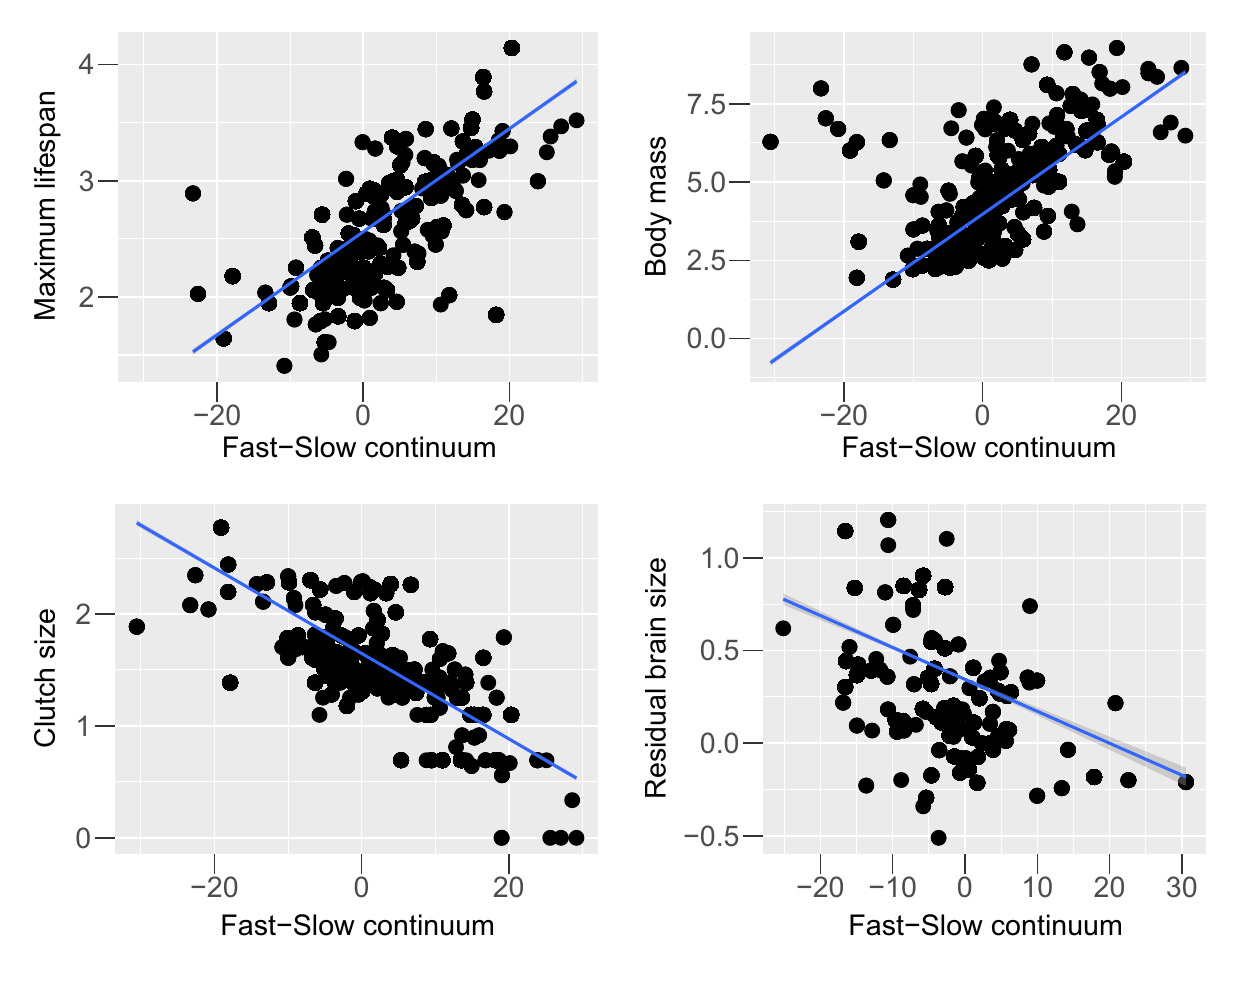
\includegraphics[width=\textwidth]{./Figures/chapter04/Fig_3.png}
\caption[Fast-slow continuum and LH traits]{Relationship of the fast-slow continuum (FS) across species with maximum lifespan,
clutch size, body mass, and residual brain size. The three first
traits have been log transformed. Residual brain size represent the
residuals of a log-log PGLS of brain volume against body mass
(i.e., positive residuals mean that the brain of the species is larger
than expected by body size and negative residuals that is smaller
than expected by body size).}\label{fig:fig4.3}
\end{figure}

Because slow-lived species tend to have disproportionally
larger brains than fast-lived species (Fig. \ref{fig:fig4.3}), the reduction in
FID observed in slow-lived species could reflect enhanced learning 
capacities. Species with larger brain residual exhibited longer
FID in rural habitats than those with smaller brain residual
(pMCMC = 0.008, Table S4), but they did not experience a more
substantial change in FID between rural and urban habitats
(Table \ref{tab:tabApp4.5}).


\begin{table}
\caption[Best model for FID]{BPMM accounting for variation in FID (response
variable, log transformed) as a function of the interaction
between habitat and the fast-slow continuum, based on information
from all regions for which both urban and rural FID observations
were available (Denmark, France, Norway, and China). The model
was run with a Gaussian structure of the errors and a non-informative
prior, the number of iterations being defined by nitt = 330,000,
burnin = 30,000 and thin = 300.}\label{tab:table4.1}
\begin{tabular}{llllll}
\toprule
            & \textbf{post mean} & \textbf{L-95\% CI} & \textbf{U-95\%} & \textbf{eff.samp} & \textbf{pMCMC} \\
\multicolumn{6}{@{}l@{}}{\textbf{Random effects}}                                       \\
Phylogeny        &               &               &        &          & -                \\ % TODO: missing values
Species          & 0.143         & 0.095         & 0.199  & 1000     & -                \\
Country          & 0.168         & 0.011         & 0.477  & 1000     & -                \\
Residual         & 0.196         & 0.190         & 0.201  & 1000     & -                \\
\multicolumn{6}{@{}l@{}}{\textbf{Fixed effects}}                                        \\
Intercept        & 3.123         & 2.567         & 3.669  & 1000     & \textless{0.001} \\
FS               & 0.024         & 0.0114        & 0.035  & 1000     & \textless{0.001} \\
Habitat:urban    & -0.321        & -0.3444       & -0.299 & 1000     & \textless{0.001} \\
Height           & 0.014         & 0.0114        & 0.017  & 1000     & \textless{0.001} \\
FS*Habitat:urban & -0.032        & -0.035        & -0.028 & 1000     & \textless{0.001} \\
\bottomrule
\end{tabular}
\end{table}


\section{Discussion}

\begin{figure}
\centering
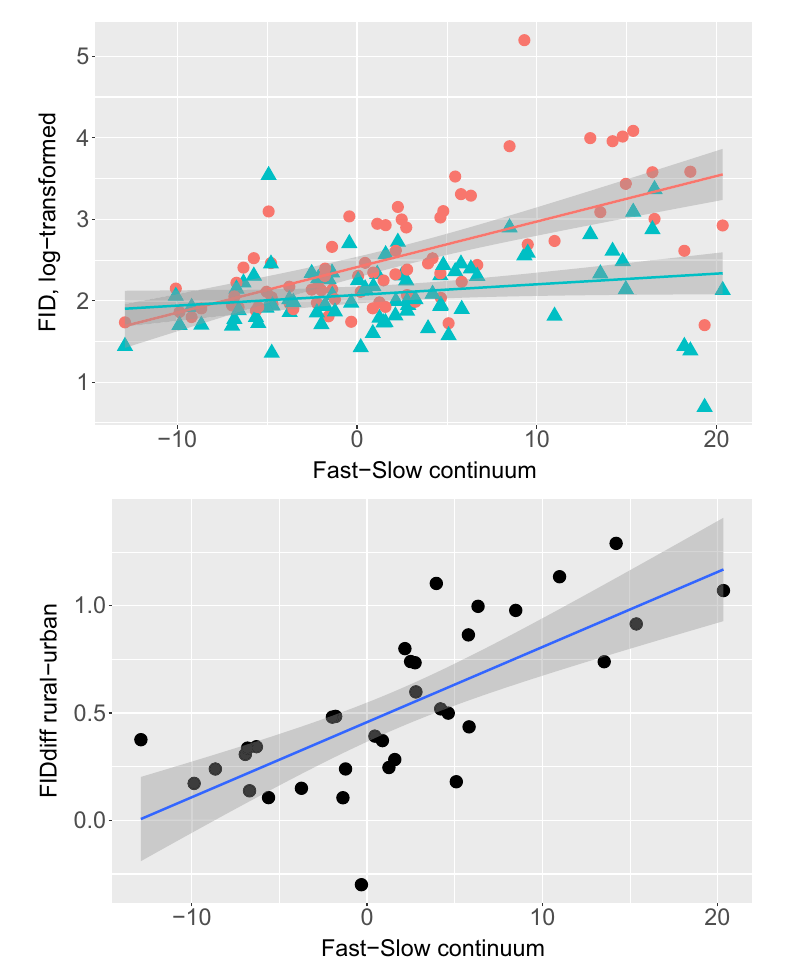
\includegraphics[width=.75\textwidth]{./Figures/chapter04/Fig_4.png}
\caption[FID and fast-slow continuum]{Above, relationship between FID and the fast-slow continuum for
urban (blue triangles) and rural (red circles) habitats. Below, difference in
FID between rural and urban habitats as a function of the fast-slow continuum.}\label{fig:fig4.4}
\end{figure}


\begin{table}
\caption[Best model for rural and urband differences in FID]{BPMM accounting for the decline in FID per species from
rural and urban habitats (response variable) a function of the fast-slow
continuum, based on information from species for which both urban and
rural FID observations were available. The decline of each species was
estimated as the $log(mean FID_{rural}) - log(mean FID_{urban})$. The model was
repeated again restricting the species to those with at least 15 FID
observations in each habitat. The models were run with a Gaussian structure
of the errors and non-informative priors. We weighted the observations
by $1/(n-3)$, being ``$n$'' the number of FID observations of the species.
The model was run with a Gaussian structure of the errors and a
non-informative prior, the number of iterations being defined by nitt =
440,000, burni = 40,000 and thin = 400.}\label{tab:table4.2}
\begin{tabular}{llllll}
\toprule
\multicolumn{6}{l}{\textbf{Model with all species}}                                                            \\
\midrule
              & \textbf{post mean} & \textbf{L-95\% CI} & \textbf{U-95\%} & \textbf{eff.samp} & \textbf{pMCMC} \\
\multicolumn{6}{@{}l@{}}{\textbf{Random effects}}                                 \\
Phylogeny             & 0.074     & 0.000     & 0.197  & 539      & -             \\
Residual              & 0.086     & 0.035     & 0.152  & 637      & -             \\
\multicolumn{6}{@{}l@{}}{\textbf{Fixed effects}}                                  \\
Intercepts         & 0.560     & 0.283     & 0.857  & 889.5    & \textless{0.001} \\
FS                 & 0.031     & 0.015     & 0.048  & 718.4    & 0.002            \\
\noalign{\bigskip}
\toprule
\multicolumn{6}{l}{\textbf{Model with  species with at least 15 FID observations per habitat}}               \\
\midrule
           & \textbf{post mean} & \textbf{L-95\% CI} & \textbf{U-95\%} & \textbf{eff.samp} & \textbf{pMCMC}  \\
\multicolumn{6}{@{}l@{}}{\textbf{Random effects}}                                 \\
Phylogeny          & 0.095     & 0.019     & 0.192  & 794      & -                \\
Residual           & 0.018     & 0.000     & 0.043  & 703.6    & -                \\
\multicolumn{6}{@{}l@{}}{\textbf{Fixed effects}}                                  \\
Intercepts         & 0.711     & 0.358     & 1.010  & 1000     & \textless{0.001} \\
FS                 & 0.021     & 0.006     & 0.036  & 878.2    & 0.006            \\
\bottomrule
\end{tabular}
\end{table}


\begin{figure}
\centering
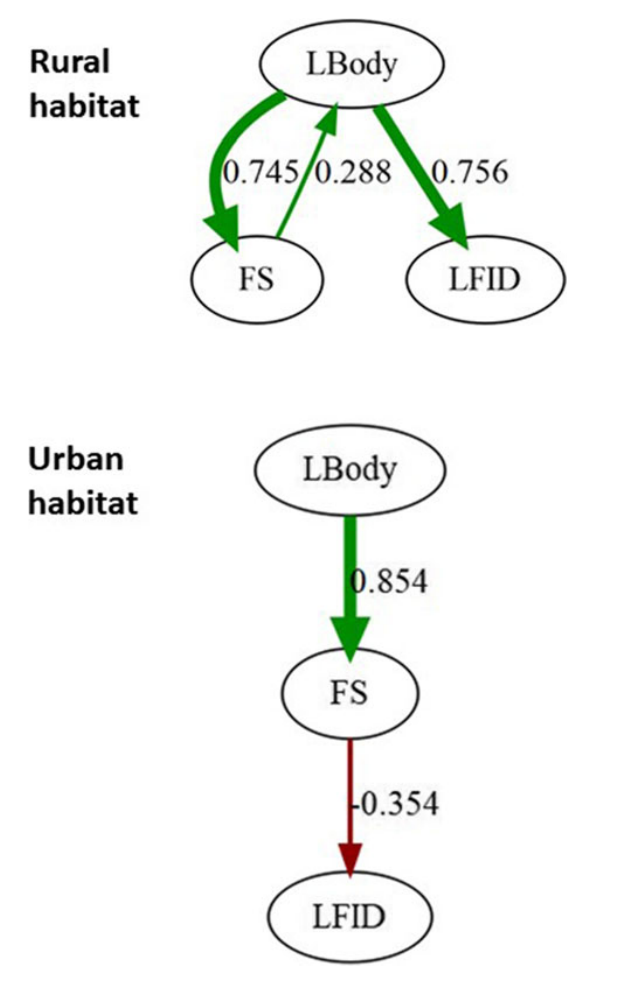
\includegraphics[width=0.5\textwidth]{./Figures/chapter04/Fig_5.png}
\caption[Phylogenetic path models for rural and urban habitats]{
Phylogenetic path model averaged over all tested models (see
Figs. S2 and S3, in the supplementary material) for rural and urban habitats,
depicting the relationship between flight initiation distance (log transformed,
LFID) and the fast-slow continuum (FS) according to differences in body mass
(LBody) across species.}\label{fig:fig4.5}
\end{figure}


Life history theory has mostly been developed under the view
that organisms are passive subjects of selection, ignoring that
behavior largely mediates how animals interact with their environment 
\citep{Sol2016}. However, recent years
have witnessed an increased appreciation that behavior can
co-vary with the life history, an idea crystalized in the POLS
concept \citep{Ricklefs2002, Reale2010a}. Our
results are in line with this new paradigm, confirming previous
suggestions and evidence that FID can be part of a POLS.

Our finding that slow-lived species tend to be more risk-averse
than fast-lived species in natural conditions fits well
with life history theory. The fitness of slow-lived animals
largely depends on ensuring a long reproductive life \citep{Stearns2000}; 
hence, individuals should favor risk-avoidance strategies
when the perception of risk is high \citep{Martin2000, Wolf2007, Hau2010a, Moller2012, Moller2013a}. 
Under this view, behavior would be a
consequence of life history. However, our analyses suggest that
the relationship between FID and the fast-slow continuum is
largely mediated by differences in body size among species.
As body size is a major determinant of the fast-slow continuum,
this does not deny the existence of a POLS. However,
larger species may also decide to flee before than smaller species
for reasons not directly induced by their life history, including
a higher likelihood to be detected by predators, lower
maneuverability to escape when attacked and higher energetic
costs associated with flight \citep{Blumstein2006}.

An animal that is unable to tolerate human presence is likely
to have problems to feed, communicate, or mate in densely
populated urban environments. This may explain why FID is
shorter in urban than in rural environments \citep{Moller2010, Moller2015a}. 
While slow-lived species showed shorter
or larger FID according to the perception of risk, fast-lived
species did not accommodate their FID to the degree of human
frequentation. The changes in FID observed in slow-lived species
may reflect plastic adjustments, selection, and/or a non-random 
sorting of individuals by behaviors that affect invasion
success. Our analyses do not allow us to distinguish between
these alternatives, although plasticity is an obvious possibility.
After detecting an approaching human, animals may decide to
ignore the threat or to flee, and cognition may be involved in
allowing informed decisions \citep{Moller2014a}. Some
animals are, for instance, able to discriminate between people
that pose a threat from people that do not \citep{Levey2009, Lee2011}. 
There is also evidence that fear of humans can
diminish when individuals are exposed to human presence for
long periods (e.g., \citet{Perals2017}). However, current
evidence that FID may be modified by habituation in the wild
remains inconclusive \citep{Moller2015}. Indeed, we did not find
evidence that enlarged brains facilitate accommodating FID to
the perception of risk, although this may simply indicate that
habituation to humans does not require the type of advanced
cognition associated with enlarged brains \citep{Overington2009}. 
Our insufficient understanding of how cognition and
neural structures affect FID is also highlighted in the fact that
we found that species with relatively larger brains exhibited
longer FID, while a previous study found the opposite pattern
\citep{Moller2014a}. As big-brained species tend to be
at the slow extreme of the fast-slow continuum, the weak effect
we found may be a mere by-product of the association between
the FID and life history. Another possibility is that sense organs
like eyes play a role in determining flight distance, with brain
size only secondarily accounting for the response \citep{Moller2014a}.

The reasons why fast-lived species did not see their FID
altered according to the perception of risk are also unclear.
While it may be argued that these species already possess
the appropriate behavior to persist in cities, it remains intriguing
why they do not increase their FID in places where interactions
with humans are rare enough to allow habituation.
Elucidating whether this reflects constrains, perhaps associated
with life history trade-offs, will represent an important avenue
for future research. The existence of substantial phylogenetic
heritability in FID, particularly when recorded in rural
habitats, is consistent with the existence of such constrains
\citep{Blomberg2003}. Further examples of possible
constrains can be found in \citet{Moller2013}, who reported that
while FID of several species of birds became shorter after a
cold winter, this was only true in resident urban populations
(frequently exposed to humans) but not in migratory or rural
populations of the same species.

Much past theoretical and empirical work on life history has
attempted to understand why organisms have diversified in a
plethora of life history strategies \citep{stearns1992evolution}. The possibility
that certain life histories offer advantages over others when it
comes to adjustment to environmental changes has also been
acknowledged (e.g., \citet{Saether2003}), but empirical
support has been more difficult to assemble (but see \citet{Sol2012a, Sol2014}). 
Similarly, little effort has focused on considering
behavior as a component of life history (e.g., \citet{Blumstein2006, Moller2012}, 
despite recent calls for the need
to integrate behavior into life history theory to better understand
how animals cope with environmental changes (reviewed in 
\citet{Sol2016}; see also \citet{Estrada2016}). Our discovery
of a POLS associated with risk-taking behavior contributes
to fill these gaps, suggesting new ways by which behavior
and life history interact to influence the response of animals to
sudden changes in their environment.


% \include{Chapters/Chapter05}
%************************************************
\chapter{General discussion and conclusions}\label{ch:discussion}
%************************************************

Life history theory explains how life history traits are selected in concert
due to constraints, trade-offs and correlated selection. The theory has evolved
from focusing on single traits such as clutch size \citep{Lack1946,Skutch1949},
explanations based on the allometric relations among life history traits and
body size \citep{Western1979}, r-K selection where traits are selected
according to the population density, including body size \citep{Pianka1970}, to
age-specific mortality \citep{Gadgil1970,Stearns1976,Charlesworth1980} and
more recently, adding behaviour as a factor interacting with the evolution
of the life history traits \citep{Ricklefs2002,Reale2010a,Sol2016}.
Despite the progress made during all these years, there is a gap in the theory
regarding the effects of the life history on the response of organisms to
environmental changes.
My thesis contributes to the advance of this field in two ways.
First, defining a demographically meaningful axes of life history variation in
birds and confirming the existence of trade-offs among traits and restrictions
for the existing combinations of life history traits (Chapter \ref{ch:LHaxes}).
Second, understanding the mechanisms by which life history interacts with
behaviour and the effects for the species dealing with new environmental
conditions (Chapters \ref{ch:LH-Behaviour model} and \ref{ch:POLS}).

\bigskip

The first objective of this thesis was to describe the diversity of life
history in birds. Despite that it is not the first time that this has been done
\citep{Saether1987,Gaillard1989,Saether2000,Jeschke2009}, my work in
chapter \ref{ch:LHaxes} supposes and advance respect the previous works. I used
newly available statistical methods that control for the phylogenetic structure
of the data by means of phylogenetic principal component analysis
\citep{Revell2009a} and phylogenetic least square regressions \citep{Ho2014}.
Also, the number of species in the compiled dataset is one order of magnitude
larger than previous works. Finally, the availability of demographic data and
the linking of it with different combinations of life history traits allowed to
objectively define the axes of life history variation that better describe
demographic features of the species instead of using traits according to their
availability.
I described the already known fast-slow axis
\citep{Stearns1983a,Saether1987,Gaillard1989,Oli2004,Dobson2007,Jeschke2009},
a iteroparity axis \citep{Gaillard1989}, an axis related to the trade-off
between offspring quantity and quality
\citep{Promislow1990,Bielby2007,Dobson2007}, and finally an axis that reflects
the lifelong productivity of the species in terms of offspring number and egg
mass produced relative to body size.
The availability of a large data base of the species position in each life
history axis opens new possibilities to understand the implications of the life
history in an evolutive and ecological framework.
Life history in birds is not as diverse as in other groups, perhaps due to the
fly constraints \citep{Gaillard1989,Healy2014}.
Future works could apply a similar methodology to more diverse groups such as
mammals for which traits and demographic data is already available
\citep{Myhrvold2015,Salguero-Gomez2016}.

\bigskip

A second objective of the thesis was to explore how life history affects the
response of species to environmental changes. Previous attempts to elucidate
the question show contradictory patterns about the effects of the fast-slow axis
on establishment success of introduced species (non significant for birds
\citep{Blackburn2009a,Sol2012a} but significant for mammals and reptiles
\citep{Capellini2015,Allen2017}), or the ability to colonize urban habitats
(non significant for birds \citep{Sol2014} but significant for mammals
\citep{Santini2019}).
As I argued in chapters \ref{ch:LH-Behaviour model} and \ref{ch:POLS}, one
possible explanation is the omission of an important factor that affects and
is affected by the species position in the fast-slow axis: the behaviour.

As a first approach to the question, I explored mechanisms by which life history
and behavior can interact by means of a theoretical individual based model
simulating the introduction of species with different life histories in a new
environment (Chapter \ref{ch:LH-Behaviour model}). The model shows that under
maladaptive scenarios, where the match of the phenotype to the environment is
insufficient, it pays to have a slow life history that increase the value of
adults over the value of offspring even at the cost of decreasing reproduction.
This is in part owing to the demographic consequences of the life-history
strategy itself and in part owing to the higher benefits of behavioural
responses for slow species in comparison to fast species.
The notion that slow animals exposed to novel environments generally gain
greater benefits from behavioural responses has been suggested in previous
studies (reviewed in \citet{Sol2016}). Animals at the ‘slow’ extreme of the
fast–slow continuum are generally believed to explore more accurately the
environment and exhibit better performance in learning than those at the ‘fast’
extreme, one reason is that they tend to have disproportionally larger brains,
which has been shown to enhance the capacity to innovate and learn
\citep{Lefebvre1997,Reader2002,Overington2009,Reader2011}. The model in chapter
\ref{ch:LH-Behaviour model} supports the idea that life history and behavior are
not independent and that studied together can help to better understand the
mechanisms by which they affect the responses to environmental changes, even
more in the context of human induced rapid environmental changes where
behavioral responses can be the key to adapt to novel conditions. Future studies
can use similar approaches to look for demographic and ecological consequences
of other relevant axes of life history variation such as iteroparity and
offspring quality-quantity as described in Chapter \ref{ch:LHaxes}. In
particular, iteroparity seems a relevant axis to adapt to novel environments as
comparative studies have shown for invasive species \citep{Sol2012a} an urban
dwellers \citep{Sol2014,Sayol2020}.

A second approach to understand how life history and behavior affect the
response to environmental changes was developed in Chapter \ref{ch:POLS}. In
this chapter I used a comparative analysis of flight initiation distances for
birds in rural and urban habitats. The results show the existence of a
peace-of-life syndrome (POLS) predicted by theory where slow-lived species tend
to be more risk-averse than fast-lived species \citep{Reale2010a}.
Furthermore, the POLS structure vanishes in urbanized environments due to
slow-lived species adjusting their flight distances based on the perception of
risk. Even though there is no evidence in birds that slow species are better
urban colonisers \citep{Sol2014}, the fact that slow species have a more plastic
behaviour supports the idea that slow species can potentially better adapt to
to environmental changes.
In the other hand, the pattern seems reverted in mammals, where species with
traits related to the fast end of the fast-slow continuum are better urban
dwellers in some groups \citep{Santini2019}.
The contradictory results about whether fast or slow strategies are better to
deal with environmental changes is still open. The fact that there is no clear
pattern in birds could be because, even though there is a fast-slow continuum
among species, the birds as a group are mostly in the slow end compared to
mammals \citep{Healy2014}.

\bigskip

Environmental changes include a wide range of processes, from land use changes
to introduction of exotic species and climate change. Each type of changes can
affect differently the resource availability and the age-specific mortality,
thus, the effects on the species and their responses or the lack of, should be
different. The nature of the changes will determine if the environment will
become more or less predictable, include novel food resources or qualitatively
different threats such as new predators for which species are not adapted.
For unpredictable environments, bet-hedging strategies can help to survive
\citep{Starrfelt2012}, but also plastic life history strategies mediated by
behavior such as the ability to module the reproductive effort by skipping
reproduction in bad years, the so called ``storage effect'' \citep{Forcada2008}.
Increased juvenile mortality by predators can be compensated by increasing
reproduction if enough resources are available \citep{Yeh2004} displacing the
species towards the fast end of the fast-slow continuum. Also, the increase of
the juvenile survival will have less impact for slow species which exhibit a
life history buffer against the effects of demographic stochasticity and are
less sensitive to changes in juvenile survival as I showed in Chapter
\ref{ch:LH-Behaviour model}.
Species can adapt to predictable changes through adjustments on the life
history \citep{Evans2005} or through behavioral plasticity mechanisms such as
learning \citep{Laundre2001,Evans2012}.
In the case of rapid changes for which there is not enough time for evolutive
responses, behavioral plastic responses may be the only way to adapt to the
new opportunities or threats \citep{Sol2009}, and there is a growing number of
evidences that behavior affects and is affected by life history \citep{Sol2016}.
Thus, when we examine how life history affects the responses to environmental
changes, we are considering not only life history mechanisms but also mechanisms
related to behavioural responses.

Probably, the answer to the question of which life history strategies are
better to respond to environment changes is context-dependent, and only by
carefully thinking about the relevant mechanisms, including behavioral
responses, for each scenario of environmental change and the taxonomic group of
study, we can refine the understanding of the effects of life history on the
ability of the species to survive to environmental changes.


\clearpage

\subpdfbookmark{Conclusions}{Conclusions}
\section*{Conclusions}

\begin{itemize}
  \item \textbf{Chapter 2:}
  \begin{itemize}
    \item Not all combinations of life history traits exist in nature. The
variation of life history traits is constrained and organized in different
axes caused by trade-off and phylogenetic constraints.
    \item One of the axes of traits' covariation is the fast-slow, described
recurrently since 1983 by a varying set of traits more often justified by the
traits data availability than for ecological reasons. This axis is related to
the survival-fecundity trade-off. Defining the fast-slow axis in a
demographically meaningful way (i.e. optimizing the correlation of the
resulting axis with the elasticity to adult survival or generation time)
allowed me to build an objective and more ecologically relevant
characterisation of the axis.
    \item The remaining variation in the life history traits once the fast-slow
is ruled out is organized in three other axes of variation, sorted by variance
explained:

    \begin{itemize}
      \item Iteroparity, describes the degree of concentration of the
reproductive effort in few or many breeding attempts.
      \item Lifelong potential productivity, related to the lifelong investment
in reproduction in terms of the number of offspring and the egg mass production
relative to the body mass.
      \item Offspring quality-quantity trade-off, sorts species along a
continuum with species with a large relative egg mass and small clutch size in
one end, and species with large clutch size and small relative egg size at the
other end.
    \end{itemize}
  \end{itemize}


  \item \textbf{Chapter 3:}
  \begin{itemize}
    \item Theoretical models help to investigate the effects and mechanisms
that affect the demography of species in novel and unknown environments.
    \item Under maladaptive scenarios where the mismatch of phenotype to the
environment is insufficient, simulations suggest that slow lived species,
for which adult have more value than offspring, have more chances to be
established.
    \item Behavioural responses interact with life history to influence the
persistence of populations in novel and unknown environments. The benefits of
learning behaviours are greater for slow strategies. Behaviours such
as skipping a reproductive event, can improve the probabilities to be
established for slow species while being detrimental for fast species. And
finally, innate responses in a context of novel environments can be beneficial
or impact negatively the probabilities to establish a population if preferences
do not match habitat quality (ecological trap), being fast strategies more
impacted by ecological traps on scenarios with higher offspring mortality and
slow strategies more impacted on scenarios with higher adult mortality.
  \end{itemize}


  \item \textbf{Chapter 4:}
  \begin{itemize}
    \item  Slow-lived species tend to have a more risk-averse behaviour than
fast-lived species.
    \item The relationship between flight initiation distance (FID) and the
fast-slow continuum is largely mediated by differences in body size among
species. Possible causes include a higher likelihood to be detected by
predators, lower maneuverability to escape when attacked and higher energetic
costs associated with flight.
    \item Flight initiation distance is shorter in urban than in rural
environments. While slow-lived species showed shorter or larger FID
according to the perception of risk, fast-lived species did not accommodate
their FID to the degree of human frequentation. The changes in FID observed in
slow-lived species may reflect plastic adjustments, selection, and/or a
non-random sorting of individuals by behaviours that affect invasion success.
  \end{itemize}


%   \item \textbf{Chapter 5:}
%   \begin{itemize}
%     \item ...
%     \item ...
%   \end{itemize}
\end{itemize}


\backmatter

\chapterstyle{default} % Reset the chapter style back to the default used for non-content chapters

%----------------------------------------------------------------------------------------
%	APPENDICES
%----------------------------------------------------------------------------------------

%************************************************
\chapter{Appendix 2: Chapter 2 - Supplementary materials}\label{ch:Appendix2.1}
%************************************************

\renewcommand{\thefigure}{A.2.\arabic{figure}}
\setcounter{figure}{0}

\renewcommand{\thetable}{A.2.\arabic{table}}
\setcounter{table}{0}

\section*{Supplementary tables}

\begin{table}[ht!]
\center
\caption[FS PCs models]{
Characteristics of the models used to select the PCs that better describe the
generation time or elasticity to the fecundity. This models are used to
define the fast-slow axes averaging and AIC weighting the PCs from the models
predicting the elasticity to the fecundity (FSe) or generation time (FSgt)
for each dataset and phylogeny. Columns describe the number of PCs included (n
PCs), the variance explained by the PCs (PCvarExp), number of traits included in
the PPCAs and the adjusted $R^{2}$ of the models predicting the elasticity to
the fecundity or the generation time. Best AIC models include only the PCs
with $\Delta AIC < 2$. The values with variability among PCs are reported as the
mean $\pm$ standard deviation. See the ESM for the complete data for all the
models.
}
\label{tab:tabApp2.1}
\begin{tabular}{@{}lllllll@{}}
\toprule
Axis & Phylogeny & Dataset & n PCs & PCvarExp & n traits & adjusted $R^{2}$\\
\midrule
\multirow{4}{*}{FSe} & \multirow{2}{*}{Ericson} & maxN & $7616$ & $0.34\pm0.08$ & $7.29\pm1.51$ & $0.36\pm0.11$\\
 &  & restricSet & $7616$ & $0.35\pm0.07$ & $7.29\pm1.51$ & $0.36\pm0.11$\\
 & \multirow{2}{*}{Hackett}& maxN & $7616$ & $0.35\pm0.07$ & $7.29\pm1.51$ & $0.36\pm0.11$\\
 &  & restricSet & $7616$ & $0.35\pm0.07$ & $7.29\pm1.51$ & $0.36\pm0.11$\\
\addlinespace
\multirow{4}{*}{FSe best AIC} & \multirow{2}{*}{Ericson} & maxN & $61$ &
$0.28\pm0.05$ & $6.02\pm1.09$ & $0.55\pm0.01$\\
 &  & restricSet & $59$ & $0.28\pm0.05$ & $6\pm1.11$ & $0.55\pm0.01$\\
 & \multirow{2}{*}{Hackett} & maxN & $55$ & $0.28\pm0.05$ & $5.98\pm1.13$ & $0.55\pm0.01$\\
 &  & restricSet & $103$ & $0.3\pm0.05$ & $5.91\pm1.2$ & $0.55\pm0.01$\\
\addlinespace
\multirow{4}{*}{FSgt} & \multirow{2}{*}{Ericson} & maxN & $7616$ & $0.34\pm0.08$ & $7.29\pm1.51$ & $0.39\pm0.06$\\
 &  & restricSet & $7616$ & $0.35\pm0.08$ & $7.29\pm1.51$ & $0.39\pm0.06$\\
 & \multirow{2}{*}{Hackett} & maxN & $7616$ & $0.35\pm0.08$ & $7.29\pm1.51$ & $0.39\pm0.05$\\
 &  & restricSet & $7616$ & $0.35\pm0.07$ & $7.29\pm1.51$ & $0.39\pm0.05$\\
\addlinespace
\multirow{4}{*}{FSgt best AIC} & \multirow{2}{*}{Ericson} & maxN & $515$ &
$0.33\pm0.07$ & $6.27\pm1.29$ & $0.48\pm0.01$\\
 &  & restricSet & $499$ & $0.33\pm0.06$ & $6.26\pm1.28$ & $0.48\pm0.01$\\
 & \multirow{2}{*}{Hackett} & maxN & $497$ & $0.33\pm0.07$ & $6.23\pm1.27$ & $0.48\pm0.01$\\
 &  & restricSet & $468$ & $0.34\pm0.06$ & $6.24\pm1.28$ & $0.48\pm0.01$\\
\bottomrule
\end{tabular}
\end{table}


\clearpage% Flush earlier floats (otherwise order might not be correct)
\begin{landscape}
\begin{table}
\center
\caption[LHT loadings of the FS axes]{
Mean $\pm$ standard deviation AIC weighted loadings of the traits for the
fast-slow axes based on models predicting generation time (FSgt) or elasticity
to the fecundity (FSe) for all trait combination PCs o using only the PCs
with AIC \textless{2} (best AIC).
}
\label{tab:tabApp2.2}
\begin{footnotesize}

\textbf{Phylogeny based on Ericson backbone}

\begin{tabular}{@{}l|rrrr|rrrr@{}}
\toprule
  & \multicolumn{4}{c|}{Restricted Set} & \multicolumn{4}{c}{Max N Set}\\
  & FSe & FSe best AIC & FSgt & FSgt best AIC & FSe & FSe best AIC & FSgt & FSgt best AIC\\
\midrule
CS & $-0.44 \pm 0.3$ & $-0.62 \pm 0.16$ & $-0.4 \pm 0.32$ & $-0.54 \pm 0.31$ & $-0.43 \pm 0.31$ & $-0.6 \pm 0.26$ & $-0.39 \pm 0.33$ & $-0.53 \pm 0.33$\\
FEC & $-0.3 \pm 0.32$ & $-0.29 \pm 0.21$ & $-0.39 \pm 0.33$ & $-0.45 \pm 0.32$ & $-0.29 \pm 0.32$ & $-0.28 \pm 0.28$ & $-0.39 \pm 0.33$ & $-0.45 \pm 0.31$\\
INC & $0.18 \pm 0.42$ & $0.01$ & $0.33 \pm 0.42$ & $0.36 \pm 0.39$ & $0.18 \pm 0.42$ & $0$ & $0.33 \pm 0.42$ & $0.36 \pm 0.39$\\
DP & $0.19 \pm 0.44$ & $0.01$ & $0.25 \pm 0.44$ & $0.14 \pm 0.35$ & $0.18 \pm 0.45$ & $0.02 \pm 0.02$ & $0.24 \pm 0.45$ & $0.14 \pm 0.38$\\
AFB & $0.24 \pm 0.31$ & $0.27 \pm 0.09$ & $0.26 \pm 0.33$ & $0.26 \pm 0.33$ & $0.23 \pm 0.32$ & $0.25 \pm 0.26$ & $0.26 \pm 0.33$ & $0.25 \pm 0.33$\\
FLE & $0.2 \pm 0.39$ & $0.15 \pm 0.06$ & $0.19 \pm 0.42$ & $0.08 \pm 0.38$ & $0.2 \pm 0.39$ & $0.13 \pm 0.06$ & $0.19 \pm 0.43$ & $0.08 \pm 0.39$\\
PRO & $-0.12 \pm 0.36$ & $-0.05 \pm 0.17$ & $-0.12 \pm 0.39$ & $0$ & $-0.11 \pm 0.36$ & $-0.05 \pm 0.18$ & $-0.11 \pm 0.4$ & $0$\\
EMR & $0.25 \pm 0.26$ & $0.48 \pm 0.13$ & $0.23 \pm 0.27$ & $0.34 \pm 0.27$ & $0.24 \pm 0.27$ & $0.43 \pm 0.22$ & $0.23 \pm 0.27$ & $0.33 \pm 0.27$\\
BM & $0.04 \pm 0.53$ & $0$ & $0.05 \pm 0.54$ & $0 \pm 0.03$ & $0.04 \pm 0.53$ & $0$ & $0.05 \pm 0.54$ & $0 \pm 0.01$\\
OV & $0 \pm 0.37$ & $-0.02 \pm 0.21$ & $0.07 \pm 0.38$ & $0.11 \pm 0.33$ & $0 \pm 0.36$ & $-0.02 \pm 0.2$ & $0.07 \pm 0.37$ & $0.11 \pm 0.31$\\
BV & $-0.12 \pm 0.53$ & $-0.35 \pm 0.23$ & $-0.02 \pm 0.49$ & $0.02 \pm 0.48$ & $0.17 \pm 0.54$ & $0.21 \pm 0.36$ & $0.09 \pm 0.52$ & $0.04 \pm 0.48$\\
LFS & $0.18 \pm 0.54$ & $0.23 \pm 0.24$ & $0.09 \pm 0.52$ & $0.04 \pm 0.48$ & $-0.11 \pm 0.53$ & $-0.28 \pm 0.37$ & $-0.01 \pm 0.48$ & $0.04 \pm 0.46$\\
RLS & $0.17 \pm 0.52$ & $0.2 \pm 0.25$ & $0.09 \pm 0.5$ & $0.06 \pm 0.46$ & $0.16 \pm 0.52$ & $0.17 \pm 0.38$ & $0.08 \pm 0.5$ & $0.03 \pm 0.45$\\
PEP & $0.05 \pm 0.38$ & $0.18 \pm 0.22$ & $-0.04 \pm 0.39$ & $-0.03 \pm 0.24$ & $0.05 \pm 0.38$ & $0.16 \pm 0.22$ & $-0.04 \pm 0.38$ & $-0.02 \pm 0.24$\\
\bottomrule
\end{tabular}

\textbf{Phylogeny based on Hackett backbone}

\begin{tabular}{@{}l|rrrr|rrrr@{}}
\toprule
  & \multicolumn{4}{c|}{Restricted Set} & \multicolumn{4}{c}{Max N Set}\\
  & FSe & FSe best AIC & FSgt & FSgt best AIC & FSe & FSe best AIC & FSgt & FSgt best AIC\\
\midrule
CS & $-0.43 \pm 0.32$ & $-0.6 \pm 0.23$ & $-0.4 \pm 0.33$ & $-0.54 \pm 0.33$ & $-0.43 \pm 0.32$ & $-0.6 \pm 0.24$ & $-0.39 \pm 0.34$ & $-0.53 \pm 0.34$\\
FEC & $-0.29 \pm 0.33$ & $-0.26 \pm 0.27$ & $-0.39 \pm 0.34$ & $-0.45 \pm 0.33$ & $-0.29 \pm 0.32$ & $-0.28 \pm 0.26$ & $-0.39 \pm 0.33$ & $-0.44 \pm 0.33$\\
INC & $0.19 \pm 0.42$ & $0.02 \pm 0.07$ & $0.33 \pm 0.41$ & $0.37 \pm 0.38$ & $0.18 \pm 0.42$ & $0$ & $0.33 \pm 0.42$ & $0.35 \pm 0.4$\\
DP & $0.19 \pm 0.45$ & $0.06 \pm 0.06$ & $0.25 \pm 0.44$ & $0.14 \pm 0.37$ & $0.18 \pm 0.45$ & $0.01$ & $0.25 \pm 0.45$ & $0.13 \pm 0.41$\\
AFB & $0.24 \pm 0.32$ & $0.25 \pm 0.09$ & $0.26 \pm 0.34$ & $0.26 \pm 0.34$ & $0.23 \pm 0.32$ & $0.27 \pm 0.2$ & $0.26 \pm 0.35$ & $0.25 \pm 0.37$\\
FLE & $0.2 \pm 0.39$ & $0.16 \pm 0.19$ & $0.19 \pm 0.42$ & $0.07 \pm 0.38$ & $0.2 \pm 0.39$ & $0.11 \pm 0.33$ & $0.2 \pm 0.41$ & $0.08 \pm 0.38$\\
PRO & $-0.12 \pm 0.36$ & $-0.04 \pm 0.16$ & $-0.12 \pm 0.37$ & $0$ & $-0.11 \pm 0.36$ & $-0.06 \pm 0.18$ & $-0.12 \pm 0.39$ & $0$\\
EMR & $0.25 \pm 0.28$ & $0.45 \pm 0.18$ & $0.23 \pm 0.28$ & $0.34 \pm 0.29$ & $0.24 \pm 0.27$ & $0.45 \pm 0.2$ & $0.23 \pm 0.28$ & $0.33 \pm 0.29$\\
BM & $0.04 \pm 0.53$ & $0$ & $0.05 \pm 0.54$ & $0 \pm 0.01$ & $0.04 \pm 0.52$ & $0$ & $0.05 \pm 0.53$ & $0 \pm 0$\\
OV & $0 \pm 0.38$ & $-0.01 \pm 0.2$ & $0.07 \pm 0.38$ & $0.12 \pm 0.34$ & $0.01 \pm 0.37$ & $-0.01 \pm 0.21$ & $0.08 \pm 0.36$ & $0.12 \pm 0.29$\\
BV & $-0.11 \pm 0.55$ & $-0.3 \pm 0.36$ & $-0.01 \pm 0.5$ & $0.02 \pm 0.49$ & $0.17 \pm 0.55$ & $0.2 \pm 0.37$ & $0.1 \pm 0.52$ & $0.05 \pm 0.48$\\
LFS & $0.17 \pm 0.56$ & $0.2 \pm 0.39$ & $0.09 \pm 0.53$ & $0.04 \pm 0.51$ & $-0.11 \pm 0.54$ & $-0.29 \pm 0.36$ & $-0.01 \pm 0.49$ & $0.03 \pm 0.47$\\
RLS & $0.16 \pm 0.54$ & $0.21 \pm 0.24$ & $0.08 \pm 0.51$ & $0.04 \pm 0.48$ & $0.16 \pm 0.54$ & $0.19 \pm 0.26$ & $0.08 \pm 0.51$ & $0.02 \pm 0.46$\\
PEP & $0.05 \pm 0.4$ & $0.16 \pm 0.23$ & $-0.05 \pm 0.39$ & $-0.03 \pm 0.25$ & $0.05 \pm 0.39$ & $0.15 \pm 0.24$ & $-0.04 \pm 0.39$ & $-0.03 \pm 0.25$\\
\bottomrule
\end{tabular}

\end{footnotesize}
\end{table}
\end{landscape}


\clearpage% Flush earlier floats (otherwise order might not be correct)
\begin{table}
\center
\caption[LHT relative importance of the FS axes]{
Relative weight of the life history traits in the fast-slow continuum. Values
range from -1 to 1, where negative values means that the absolute value of the
trait loadings are lower than expected by the frequency of the trait and
positive values for traits with higher loadings than expected by the frequency
of the trait in the selected PPCAs (see main text for details). The loadings and
frequencies come from selected PCs that better predict elasticities to the
fecundity (FSe) or generation time (FSgt), weighted by the AIC based weight
of the models taking all or only the models with $\Delta AIC < 2$ (best AIC).
}
\label{tab:tabApp2.3}
\begin{footnotesize}

\textbf{Phylogeny based on Ericson backbone}

\begin{tabular}{@{}l|rrrr|rrrr@{}}
\toprule
  & \multicolumn{4}{c|}{Restricted Set} & \multicolumn{4}{c}{Max N Set}\\
  & FSe & FSe best AIC & FSgt & FSgt best AIC & FSe & FSe best AIC & FSgt & FSgt best AIC\\
\midrule
CS & 0.05 & 0.05 & 0.05 & 0.09 & 0.05 & 0.06 & 0.05 & 0.09\\
FEC & 0.03 & -0.01 & 0.05 & 0.07 & 0.03 & 0.00 & 0.05 & 0.08\\
INC & 0.02 & 0.00 & 0.04 & 0.04 & 0.02 & 0.00 & 0.04 & 0.05\\
DP & 0.02 & 0.00 & 0.03 & 0.01 & 0.02 & 0.00 & 0.03 & 0.01\\
AFB & 0.01 & 0.01 & 0.02 & 0.01 & 0.01 & 0.01 & 0.02 & 0.01\\
FLE & 0.02 & 0.00 & 0.01 & 0.00 & 0.02 & 0.01 & 0.02 & -0.01\\
PRO & 0.00 & -0.01 & 0.01 & 0.00 & 0.00 & -0.01 & 0.01 & 0.00\\
EMR & 0.01 & 0.03 & 0.00 & 0.01 & 0.00 & 0.02 & 0.00 & 0.01\\
BM & 0.00 & 0.00 & 0.00 & 0.00 & 0.00 & 0.00 & 0.00 & 0.00\\
OV & -0.04 & -0.03 & -0.03 & -0.01 & -0.04 & -0.03 & -0.03 & -0.01\\
BV & -0.02 & 0.01 & -0.05 & -0.06 & -0.01 & 0.01 & -0.05 & -0.08\\
LFS & -0.01 & 0.01 & -0.05 & -0.08 & -0.02 & 0.00 & -0.05 & -0.05\\
RLS & -0.01 & 0.01 & -0.05 & -0.07 & -0.01 & 0.00 & -0.05 & -0.08\\
PEP & -0.06 & -0.07 & -0.04 & -0.02 & -0.06 & -0.07 & -0.04 & -0.03\\
\bottomrule
\end{tabular}

\textbf{Phylogeny based on Hackett backbone}

\begin{tabular}{@{}l|rrrr|rrrr@{}}
\toprule
  & \multicolumn{4}{c|}{Restricted Set} & \multicolumn{4}{c}{Max N Set}\\
  & FSe & FSe best AIC & FSgt & FSgt best AIC & FSe & FSe best AIC & FSgt & FSgt best AIC\\
\midrule
CS & 0.05 & 0.05 & 0.05 & 0.09 & 0.05 & 0.06 & 0.05 & 0.09\\
FEC & 0.03 & 0.00 & 0.05 & 0.07 & 0.03 & 0.00 & 0.05 & 0.08\\
INC & 0.02 & 0.00 & 0.04 & 0.05 & 0.02 & 0.00 & 0.04 & 0.04\\
DP & 0.02 & 0.00 & 0.03 & 0.01 & 0.02 & 0.00 & 0.03 & 0.01\\
AFB & 0.02 & 0.01 & 0.02 & 0.01 & 0.02 & 0.01 & 0.02 & 0.01\\
FLE & 0.02 & 0.00 & 0.02 & -0.01 & 0.02 & -0.01 & 0.02 & 0.00\\
PRO & 0.00 & -0.01 & 0.02 & 0.00 & 0.00 & -0.01 & 0.01 & 0.00\\
EMR & 0.01 & 0.03 & -0.01 & 0.01 & 0.00 & 0.03 & -0.01 & 0.01\\
BM & 0.00 & 0.00 & 0.00 & 0.00 & 0.00 & 0.00 & 0.00 & 0.00\\
OV & -0.04 & -0.03 & -0.03 & -0.01 & -0.04 & -0.03 & -0.03 & -0.01\\
BV & -0.02 & 0.01 & -0.05 & -0.05 & -0.01 & 0.01 & -0.05 & -0.07\\
LFS & -0.01 & 0.00 & -0.05 & -0.08 & -0.02 & 0.00 & -0.05 & -0.05\\
RLS & -0.02 & 0.01 & -0.05 & -0.08 & -0.02 & 0.01 & -0.05 & -0.09\\
PEP & -0.06 & -0.07 & -0.04 & -0.02 & -0.06 & -0.08 & -0.04 & -0.02\\
\bottomrule
\end{tabular}

\end{footnotesize}
\end{table}


\clearpage% Flush earlier floats (otherwise order might not be correct)
\begin{table}
\center
\caption[PC clusters]{
Characteristics of the PCs in each cluster defining other axes than the
fast-slow for the life history variation. Columns describe the variance
explained by the PCs (PCvarExp), number of traits included in the PPCAs
(nTraits), the number of PCs (nPCs) and the main trait. The values with
variability among PCs are reported as the mean $\pm$ standard deviation.
}
\label{tab:tabApp2.4}

\begin{tabular}{llrrr}
\toprule
Group & Axis & PCvarExp & nTraits & nPCs\\
\midrule
\multicolumn{5}{@{}l@{}}{\textbf{Ericson-maxN}} \\
\midrule
\multirow{4}{*}{Iteroparity} & grCor0.7\_11 & $0.36 \pm 0.09$ & $7.41 \pm 1.4$ & 780\\
 & grCor0.7\_30 & $0.37 \pm 0.1$ & $7.53 \pm 1.49$ & 521\\
 & grCor0.75\_1 & $0.4 \pm 0.1$ & $7.42 \pm 1.38$ & 577\\
 & grCor0.8\_63 & $0.41 \pm 0.09$ & $7.71 \pm 1.51$ & 591\\
\addlinespace
\multirow{3}{*}{Offspring Q-Q} & grCor0.7\_21 & $0.14 \pm 0.02$ & $8.1 \pm 1.23$ & 828\\
 & grCor0.8\_23 & $0.15 \pm 0.03$ & $7.81 \pm 1.36$ & 756\\
 & grCor0.8\_31 & $0.14 \pm 0.02$ & $8.27 \pm 1.22$ & 623\\
\addlinespace
Lifelong prod. & grCor0.75\_7 & $0.4 \pm 0.06$ & $7.33 \pm 1.37$ & 529\\
\midrule
\addlinespace
\multicolumn{5}{@{}l@{}}{\textbf{Ericson-Restricted Set}} \\
\midrule
\multirow{4}{*}{Iteroparity} & grCor0.7\_1 & $0.38 \pm 0.1$ & $7.47 \pm 1.44$ & 649\\
 & grCor0.7\_13 & $0.36 \pm 0.09$ & $7.53 \pm 1.36$ & 793\\
 & grCor0.75\_1 & $0.38 \pm 0.1$ & $7.63 \pm 1.39$ & 546\\
 & grCor0.8\_60 & $0.41 \pm 0.09$ & $7.77 \pm 1.47$ & 623\\
\addlinespace
\multirow{3}{*}{Offspring Q-Q} & grCor0.7\_17 & $0.15 \pm 0.03$ & $7.65 \pm 1.27$ & 736\\
 & grCor0.7\_19 & $0.15 \pm 0.03$ & $7.72 \pm 1.4$ & 487\\
 & grCor0.8\_22 & $0.15 \pm 0.03$ & $7.7 \pm 1.32$ & 601\\
\addlinespace
Lifelong prod. & grCor0.8\_5 & $0.39 \pm 0.06$ & $7.47 \pm 1.41$ & 674\\
\midrule
\addlinespace
\multicolumn{5}{@{}l@{}}{\textbf{Hackett-maxN}} \\
\midrule
\multirow{3}{*}{Iteroparity} & grCor0.7\_11 & $0.36 \pm 0.08$ & $7.39 \pm 1.4$ & 855\\
 & grCor0.75\_1 & $0.37 \pm 0.11$ & $7.53 \pm 1.53$ & 477\\
 & grCor0.75\_11 & $0.4 \pm 0.07$ & $7.38 \pm 1.39$ & 545\\
\addlinespace
\multirow{2}{*}{Offspring Q-Q} & grCor0.8\_25 & $0.15 \pm 0.03$ & $7.89 \pm 1.31$ & 645\\
 & grCor0.85\_31 & $0.15 \pm 0.03$ & $7.88 \pm 1.35$ & 533\\
\addlinespace
Lifelong prod. & grCor0.75\_5 & $0.38 \pm 0.06$ & $7.5 \pm 1.43$ & 691\\
\midrule
\addlinespace
\multicolumn{5}{@{}l@{}}{\textbf{Hackett-Restricted Set}} \\
\midrule
\multirow{3}{*}{Iteroparity} & grCor0.7\_43 & $0.4 \pm 0.09$ & $7.77 \pm 1.49$ & 672\\
 & grCor0.75\_18 & $0.37 \pm 0.09$ & $7.47 \pm 1.38$ & 487\\
 & grCor0.75\_29 & $0.33 \pm 0.08$ & $7.84 \pm 1.43$ & 586\\
\addlinespace
\multirow{4}{*}{Offspring Q-Q} & grCor0.7\_17 & $0.15 \pm 0.03$ & $7.9 \pm 1.29$ & 831\\
 & grCor0.75\_19 & $0.15 \pm 0.03$ & $8.01 \pm 1.3$ & 710\\
 & grCor0.8\_24 & $0.15 \pm 0.03$ & $7.82 \pm 1.43$ & 514\\
\addlinespace
Lifelong prod. & grCor0.8\_5 & $0.4 \pm 0.05$ & $7.41 \pm 1.33$ & 522\\
\bottomrule
\end{tabular}
\end{table}



\clearpage% Flush earlier floats (otherwise order might not be correct)
\begin{landscape}
\begin{table}
\center
\caption[LHT loadings of the alternative axes]{
Mean $\pm$ standard deviation of the loadings of the traits for clusters of
similar significant PCs (Eigenvalue \textgreater{1}) not selected for the
fast-slow axes. Each group contains PCs with scores correlation greater than the
correlation specified in the group name (e.g. gr0.8 means correlation
\textgreater{0.8}). The main trait of the axes appear among brackets,
following the conventions in the table \ref{tab:table2.1}.
}
\label{tab:tabApp2.5}
\begin{footnotesize}

\textbf{Phylogeny based on Ericson backbone and max N dataset}

\begin{tabular}{@{}l|rrrr|rrr|r@{}}
\toprule
 & \multicolumn{4}{c|}{Iteroparity} & \multicolumn{3}{c|}{Offspring Q-Q} & \multicolumn{1}{c}{Lifelong prod.}\\
 & gr0.7\_11 & gr0.7\_30 & gr0.75\_1 & gr0.8\_63 & gr0.7\_21 & gr0.8\_23 & gr0.8\_31 & gr0.75\_7\\
\midrule
BV & $-0.45 \pm 0.01$ & $-0.55 \pm 0.04$ & $-0.6 \pm 0.07$ & $-0.58 \pm 0.01$ & $-0.02 \pm 0.08$ & $0.01 \pm 0.1$ & $-0.01 \pm 0.02$ & $0.22 \pm 0.13$\\
OV & $-0.46 \pm 0.03$ & $-0.29 \pm 0.02$ & $-0.41 \pm 0.09$ & $-0.56 \pm 0.01$ & $0.02 \pm 0.08$ & $0.02 \pm 0.11$ & $0.02 \pm 0.01$ & $0.45 \pm 0.06$\\
LFS & $0.45 \pm 0.04$ & $0.73 \pm 0.08$ & $0.69 \pm 0.12$ & $0.56 \pm 0.03$ & $0.02 \pm 0.12$ & $-0.05 \pm 0.11$ & $0.01 \pm 0.03$ & $-0.27 \pm 0.15$\\
RLS & $0.47 \pm 0.03$ & $0.73 \pm 0.08$ & $0.66 \pm 0.12$ & $0.59 \pm 0.02$ & $0.02 \pm 0.12$ & $-0.06 \pm 0.11$ & $0.01 \pm 0.03$ & $-0.3 \pm 0.15$\\
EMR & $-0.04 \pm 0.07$ & $0.04 \pm 0.09$ & $0.01 \pm 0.05$ & $0 \pm 0.06$ & $0.86 \pm 0.04$ & $0.91 \pm 0.05$ & $0.87 \pm 0.05$ & $0.05 \pm 0.08$\\
BM & $-0.02 \pm 0.09$ & $0.11 \pm 0.08$ & $0.06 \pm 0.09$ & $0.03 \pm 0.06$ & $-0.21 \pm 0.08$ & $-0.01 \pm 0.08$ & $-0.15 \pm 0.05$ & $0.04 \pm 0.09$\\
PRO & $0.24 \pm 0.11$ & $0.04 \pm 0.1$ & $0.06 \pm 0.09$ & $0.14 \pm 0.06$ & $0.1 \pm 0.09$ & $0.4 \pm 0.07$ & $0.13 \pm 0.06$ & $-0.5 \pm 0.11$\\
PEP & $0.52 \pm 0.03$ & $0.46 \pm 0.02$ & $0.63 \pm 0.08$ & $0.77 \pm 0.02$ & $0.13 \pm 0.08$ & $0.07 \pm 0.14$ & $0.13 \pm 0.02$ & $-0.74 \pm 0.06$\\
AFB & $-0.09 \pm 0.07$ & $0.06 \pm 0.05$ & $0.01 \pm 0.14$ & $-0.03 \pm 0.04$ & $0.03 \pm 0.11$ & $0.09 \pm 0.09$ & $0.06 \pm 0.04$ & $0.18 \pm 0.07$\\
CS & $0.26 \pm 0.08$ & $0.09 \pm 0.12$ & $0.1 \pm 0.09$ & $0.15 \pm 0.06$ & $-0.23 \pm 0.09$ & $-0.1 \pm 0.09$ & $-0.21 \pm 0.06$ & $-0.48 \pm 0.08$\\
FEC & $0.43 \pm 0.08$ & $0.15 \pm 0.09$ & $0.25 \pm 0.1$ & $0.38 \pm 0.05$ & $-0.14 \pm 0.1$ & $0.01 \pm 0.12$ & $-0.15 \pm 0.05$ & $-0.55 \pm 0.08$\\
DP & $-0.09 \pm 0.05$ & $0.11 \pm 0.06$ & $0.05 \pm 0.07$ & $-0.01 \pm 0.04$ & $-0.1 \pm 0.07$ & $0.02 \pm 0.1$ & $-0.12 \pm 0.04$ & $0.12 \pm 0.08$\\
FLE & $-0.06 \pm 0.05$ & $0.12 \pm 0.06$ & $0.06 \pm 0.07$ & $0.01 \pm 0.04$ & $-0.19 \pm 0.07$ & $-0.03 \pm 0.11$ & $-0.21 \pm 0.04$ & $0.1 \pm 0.07$\\
INC & $-0.12 \pm 0.04$ & $0.06 \pm 0.05$ & $0.01 \pm 0.07$ & $-0.04 \pm 0.03$ & $0.02 \pm 0.04$ & $0.12 \pm 0.09$ & $0.04 \pm 0.03$ & $0.17 \pm 0.09$\\
\bottomrule
\end{tabular}

\textbf{Phylogeny based on Ericson backbone and restricted dataset}

\begin{tabular}{@{}l|rrrr|rrr|r@{}}
\toprule
 & \multicolumn{4}{c|}{Iteroparity} & \multicolumn{3}{c|}{Offspring Q-Q} & \multicolumn{1}{c}{Lifelong prod.}\\
 & gr0.7\_1 & gr0.7\_13 & gr0.75\_1 & gr0.8\_60 & gr0.7\_17 & gr0.7\_19 & gr0.8\_22 & gr0.8\_5\\
\midrule
BV & $-0.49 \pm 0.01$ & $-0.42 \pm 0.12$ & $-0.47 \pm 0.1$ & $-0.58 \pm 0.02$ & $0 \pm 0.05$ & $0 \pm 0.01$ & $0 \pm 0.13$ & $-0.28 \pm 0.15$\\
OV & $-0.55 \pm 0.01$ & $-0.41 \pm 0.07$ & $-0.54 \pm 0.11$ & $-0.58 \pm 0.01$ & $0.02 \pm 0.03$ & $0.02 \pm 0.01$ & $0.02 \pm 0.1$ & $-0.36 \pm 0.14$\\
LFS & $0.69 \pm 0.03$ & $0.45 \pm 0.16$ & $0.71 \pm 0.13$ & $0.56 \pm 0.04$ & $-0.03 \pm 0.09$ & $-0.04 \pm 0.03$ & $-0.03 \pm 0.14$ & $0.21 \pm 0.14$\\
RLS & $0.65 \pm 0.03$ & $0.48 \pm 0.16$ & $0.66 \pm 0.14$ & $0.58 \pm 0.03$ & $-0.03 \pm 0.09$ & $-0.05 \pm 0.17$ & $-0.03 \pm 0.14$ & $0.24 \pm 0.14$\\
EMR & $-0.01 \pm 0.08$ & $-0.05 \pm 0.06$ & $-0.01 \pm 0.03$ & $-0.01 \pm 0.04$ & $0.89 \pm 0.07$ & $0.89 \pm 0.08$ & $0.9 \pm 0.04$ & $-0.06 \pm 0.09$\\
BM & $0.07 \pm 0.06$ & $-0.03 \pm 0.12$ & $0.08 \pm 0.06$ & $0.03 \pm 0.05$ & $-0.13 \pm 0.08$ & $0 \pm 0.07$ & $-0.13 \pm 0.06$ & $-0.07 \pm 0.06$\\
PRO & $0.08 \pm 0.05$ & $0.3 \pm 0.09$ & $0.08 \pm 0.08$ & $0.15 \pm 0.07$ & $0.26 \pm 0.12$ & $0.38 \pm 0.07$ & $0.3 \pm 0.08$ & $0.57 \pm 0.08$\\
PEP & $0.45 \pm 0.02$ & $0.57 \pm 0.07$ & $0.53 \pm 0.12$ & $0.77 \pm 0.02$ & $0.1 \pm 0.02$ & $0.09 \pm 0.02$ & $0.1 \pm 0.12$ & $0.74 \pm 0.19$\\
AFB & $0.01 \pm 0.03$ & $-0.1 \pm 0.08$ & $0.01 \pm 0.08$ & $-0.03 \pm 0.04$ & $0.01 \pm 0.06$ & $0.12 \pm 0.04$ & $0.02 \pm 0.09$ & $-0.22 \pm 0.09$\\
CS & $0.16 \pm 0.09$ & $0.3 \pm 0.08$ & $0.17 \pm 0.09$ & $0.16 \pm 0.06$ & $-0.16 \pm 0.11$ & $-0.03 \pm 0.09$ & $-0.18 \pm 0.09$ & $0.37 \pm 0.11$\\
FEC & $0.25 \pm 0.06$ & $0.39 \pm 0.08$ & $0.26 \pm 0.12$ & $0.37 \pm 0.05$ & $-0.09 \pm 0.09$ & $0.02 \pm 0.09$ & $-0.07 \pm 0.12$ & $0.59 \pm 0.13$\\
DP & $0.05 \pm 0.04$ & $-0.1 \pm 0.1$ & $0.05 \pm 0.05$ & $-0.01 \pm 0.05$ & $-0.04 \pm 0.07$ & $0.04 \pm 0.05$ & $-0.04 \pm 0.07$ & $-0.19 \pm 0.09$\\
FLE & $0.06 \pm 0.04$ & $-0.07 \pm 0.1$ & $0.06 \pm 0.05$ & $0 \pm 0.04$ & $-0.11 \pm 0.06$ & $-0.01 \pm 0.05$ & $-0.08 \pm 0.09$ & $-0.15 \pm 0.11$\\
INC & $0.01 \pm 0.03$ & $-0.13 \pm 0.09$ & $0 \pm 0.06$ & $-0.05 \pm 0.04$ & $0.03 \pm 0.06$ & $0.13 \pm 0.04$ & $0.04 \pm 0.08$ & $-0.22 \pm 0.07$\\
\bottomrule
\end{tabular}
\end{footnotesize}
\end{table}

% Pretend that the next table is the continuation of the former
% \addtocounter{table}{-1}

\clearpage% Flush earlier floats (otherwise order might not be correct)

\begin{table}
\center
\begin{footnotesize}

\textbf{Phylogeny based on Hackett backbone and max N dataset}

\begin{tabular}{@{}l|rrr|rr|r@{}}
\toprule
 & \multicolumn{3}{c|}{Iteroparity} & \multicolumn{2}{c|}{Offspring Q-Q} & \multicolumn{1}{c}{Lifelong prod.}\\
 & gr0.7\_11 & gr0.75\_1 & gr0.75\_11 & gr0.8\_25 & gr0.85\_31 & gr0.75\_5\\
\midrule
BV & $-0.37 \pm 0.11$ & $-0.57 \pm 0.13$ & $-0.44 \pm 0.11$ & $0.01 \pm 0.04$ & $0.01 \pm 0.02$ & $-0.29 \pm 0.04$\\
OV & $-0.5 \pm 0.1$ & $-0.6 \pm 0.08$ & $-0.59 \pm 0.1$ & $0.03 \pm 0.02$ & $0.02 \pm 0.01$ & $-0.25 \pm 0.02$\\
LFS & $0.45 \pm 0.12$ & $0.56 \pm 0.17$ & $0.39 \pm 0.11$ & $-0.04 \pm 0.08$ & $-0.06 \pm 0.03$ & $0.21 \pm 0.07$\\
RLS & $0.48 \pm 0.13$ & $0.57 \pm 0.17$ & $0.43 \pm 0.11$ & $-0.04 \pm 0.08$ & $-0.07 \pm 0.03$ & $0.23 \pm 0.07$\\
EMR & $-0.06 \pm 0.03$ & $-0.02 \pm 0.07$ & $-0.03 \pm 0.05$ & $0.9 \pm 0.1$ & $0.9 \pm 0.08$ & $-0.06 \pm 0.07$\\
BM & $-0.02 \pm 0.06$ & $0.06 \pm 0.13$ & $-0.03 \pm 0.04$ & $-0.12 \pm 0.1$ & $0 \pm 0.06$ & $-0.14 \pm 0.06$\\
PRO & $0.23 \pm 0.07$ & $0.11 \pm 0.1$ & $0.29 \pm 0.08$ & $0.26 \pm 0.1$ & $0.42 \pm 0.05$ & $0.59 \pm 0.07$\\
PEP & $0.52 \pm 0.11$ & $0.4 \pm 0.07$ & $0.73 \pm 0.12$ & $0.12 \pm 0.02$ & $0.06 \pm 0.02$ & $0.71 \pm 0.02$\\
AFB & $-0.09 \pm 0.1$ & $0 \pm 0.08$ & $-0.1 \pm 0.08$ & $0.04 \pm 0.06$ & $0.1 \pm 0.04$ & $-0.23 \pm 0.05$\\
CS & $0.28 \pm 0.07$ & $0.14 \pm 0.09$ & $0.24 \pm 0.07$ & $-0.18 \pm 0.09$ & $-0.05 \pm 0.09$ & $0.35 \pm 0.09$\\
FEC & $0.46 \pm 0.11$ & $0.37 \pm 0.08$ & $0.53 \pm 0.12$ & $-0.08 \pm 0.08$ & $0.03 \pm 0.06$ & $0.48 \pm 0.06$\\
DP & $-0.09 \pm 0.06$ & $0.03 \pm 0.1$ & $-0.08 \pm 0.09$ & $-0.04 \pm 0.07$ & $0.03 \pm 0.04$ & $-0.23 \pm 0.07$\\
FLE & $-0.07 \pm 0.07$ & $0.05 \pm 0.1$ & $-0.07 \pm 0.09$ & $-0.13 \pm 0.07$ & $-0.02 \pm 0.04$ & $-0.19 \pm 0.06$\\
INC & $-0.12 \pm 0.07$ & $-0.02 \pm 0.09$ & $-0.11 \pm 0.08$ & $0.04 \pm 0.05$ & $0.14 \pm 0.03$ & $-0.27 \pm 0.06$\\
\bottomrule
\end{tabular}

\textbf{Phylogeny based on Hacket backbone and restricted dataset}

\begin{tabular}{@{}l|rrr|rrr|r@{}}
\toprule
 & \multicolumn{3}{c|}{Iteroparity} & \multicolumn{3}{c|}{Offspring Q-Q} & \multicolumn{1}{c}{Lifelong prod.}\\
 & gr0.7\_43 & gr0.75\_18 & gr0.75\_29 & gr0.7\_17 & gr0.75\_19 & gr0.8\_24 & gr0.8\_5\\
\midrule
BV & $-0.55 \pm 0.12$ & $-0.57 \pm 0.01$ & $-0.32 \pm 0.14$ & $0.01 \pm 0.01$ & $0 \pm 0.04$ & $0.01 \pm 0.12$ & $-0.25 \pm 0.08$\\
OV & $-0.48 \pm 0.1$ & $-0.45 \pm 0.02$ & $-0.39 \pm 0.08$ & $0.02 \pm 0.01$ & $0.02 \pm 0.01$ & $0.03 \pm 0.1$ & $-0.33 \pm 0.09$\\
LFS & $0.65 \pm 0.12$ & $0.43 \pm 0.04$ & $0.64 \pm 0.16$ & $-0.03 \pm 0.04$ & $-0.02 \pm 0.06$ & $-0.06 \pm 0.12$ & $0.16 \pm 0.1$\\
RLS & $0.62 \pm 0.11$ & $0.48 \pm 0.04$ & $0.61 \pm 0.16$ & $-0.03 \pm 0.04$ & $-0.02 \pm 0.07$ & $-0.07 \pm 0.13$ & $0.19 \pm 0.1$\\
EMR & $0 \pm 0.06$ & $-0.03 \pm 0.06$ & $0.02 \pm 0.06$ & $0.89 \pm 0.05$ & $0.9 \pm 0.05$ & $0.9 \pm 0.03$ & $-0.06 \pm 0.03$\\
BM & $0.03 \pm 0.06$ & $-0.01 \pm 0.08$ & $0.12 \pm 0.13$ & $-0.12 \pm 0.05$ & $-0.14 \pm 0.07$ & $0 \pm 0.07$ & $-0.1 \pm 0.07$\\
PRO & $0.12 \pm 0.08$ & $0.29 \pm 0.08$ & $0.06 \pm 0.08$ & $0.28 \pm 0.06$ & $0.27 \pm 0.1$ & $0.41 \pm 0.09$ & $0.68 \pm 0.1$\\
PEP & $0.82 \pm 0.13$ & $0.6 \pm 0.04$ & $0.59 \pm 0.07$ & $0.11 \pm 0.02$ & $0.12 \pm 0.02$ & $0.07 \pm 0.11$ & $0.78 \pm 0.09$\\
AFB & $-0.01 \pm 0.07$ & $-0.07 \pm 0.05$ & $0.05 \pm 0.08$ & $0.04 \pm 0.04$ & $0.05 \pm 0.04$ & $0.11 \pm 0.1$ & $-0.22 \pm 0.09$\\
CS & $0.15 \pm 0.08$ & $0.17 \pm 0.08$ & $0.14 \pm 0.07$ & $-0.21 \pm 0.08$ & $-0.22 \pm 0.08$ & $-0.03 \pm 0.11$ & $0.42 \pm 0.11$\\
FEC & $0.32 \pm 0.13$ & $0.4 \pm 0.09$ & $0.21 \pm 0.06$ & $-0.06 \pm 0.06$ & $-0.06 \pm 0.07$ & $0.03 \pm 0.11$ & $0.52 \pm 0.12$\\
DP & $0 \pm 0.08$ & $-0.07 \pm 0.07$ & $0.13 \pm 0.1$ & $-0.05 \pm 0.05$ & $-0.05 \pm 0.05$ & $0.04 \pm 0.07$ & $-0.18 \pm 0.06$\\
FLE & $0.02 \pm 0.09$ & $-0.05 \pm 0.06$ & $0.14 \pm 0.1$ & $-0.13 \pm 0.05$ & $-0.12 \pm 0.05$ & $-0.02 \pm 0.08$ & $-0.16 \pm 0.06$\\
INC & $-0.03 \pm 0.07$ & $-0.1 \pm 0.06$ & $0.06 \pm 0.1$ & $0.04 \pm 0.05$ & $0.04 \pm 0.04$ & $0.14 \pm 0.07$ & $-0.22 \pm 0.05$\\
\bottomrule
\end{tabular}

\end{footnotesize}
\end{table}
\end{landscape}


\clearpage% Flush earlier floats (otherwise order might not be correct)
\begin{landscape}
\begin{table}
\center
\caption[LHT relative importance of the alternative axes]{
Relative weights of the life history traits for each axes described in the
table \ref{tab:tabApp2.4}. Values range from -1 to 1, where negative values
means that the absolute value of the trait loadings are lower than expected by
the frequency of the trait and positive values for traits with higher loadings
than expected by the frequency of the trait in the selected PPCAs (see main
text for details).
}
\label{tab:tabApp2.6}
\begin{footnotesize}

\textbf{Phylogeny based on Ericson backbone and max N dataset}

\begin{tabular}{@{}l|rrrr|rrr|r@{}}
\toprule
 & \multicolumn{4}{c|}{Iteroparity} & \multicolumn{3}{c|}{Offspring Q-Q} & \multicolumn{1}{c}{Lifelong prod.}\\
 & gr0.7\_11 & gr0.7\_30 & gr0.75\_1 & gr0.8\_63 & gr0.7\_21 & gr0.8\_23 & gr0.8\_31 & gr0.75\_7\\
\midrule
BV & 0.05 & 0.08 & 0.08 & 0.07 & -0.05 & -0.05 & -0.05 & 0.01\\
OV & 0.06 & 0.04 & 0.06 & 0.07 & -0.04 & -0.05 & -0.04 & 0.04\\
LFS & 0.04 & 0.10 & 0.09 & 0.06 & -0.06 & -0.05 & -0.06 & -0.01\\
RLS & 0.04 & 0.10 & 0.09 & 0.06 & -0.06 & -0.05 & -0.06 & 0.00\\
EMR & -0.05 & -0.06 & -0.07 & -0.06 & 0.29 & 0.35 & 0.29 & -0.06\\
BM & -0.05 & -0.02 & -0.03 & -0.05 & 0.02 & 0.00 & 0.00 & -0.01\\
PRO & 0.00 & -0.04 & -0.02 & -0.02 & 0.01 & 0.09 & 0.01 & 0.02\\
PEP & 0.07 & 0.06 & 0.08 & 0.09 & -0.02 & -0.02 & -0.03 & 0.06\\
AFB & -0.04 & -0.05 & -0.06 & -0.05 & -0.06 & -0.03 & -0.04 & -0.03\\
CS & 0.00 & -0.06 & -0.03 & -0.01 & 0.04 & -0.02 & 0.04 & 0.01\\
FEC & 0.02 & -0.04 & -0.02 & 0.00 & 0.00 & -0.09 & 0.00 & 0.04\\
DP & -0.04 & -0.03 & -0.05 & -0.06 & -0.02 & -0.05 & -0.03 & -0.02\\
FLE & -0.05 & -0.03 & -0.05 & -0.06 & 0.01 & -0.04 & 0.01 & -0.03\\
INC & -0.04 & -0.05 & -0.07 & -0.05 & -0.05 & -0.01 & -0.04 & -0.02\\
\bottomrule
\end{tabular}

\textbf{Phylogeny based on Ericson backbone and restricted dataset}

\begin{tabular}{@{}l|rrrr|rrr|r@{}}
\toprule
 & \multicolumn{4}{c|}{Iteroparity} & \multicolumn{3}{c|}{Offspring Q-Q} & \multicolumn{1}{c}{Lifelong prod.}\\
 & gr0.7\_1 & gr0.7\_13 & gr0.75\_1 & gr0.8\_60 & gr0.7\_17 & gr0.7\_19 & gr0.8\_22 & gr0.8\_5\\
\midrule
BV & 0.07 & 0.05 & 0.07 & 0.07 & -0.05 & -0.06 & -0.05 & 0.01\\
OV & 0.08 & 0.05 & 0.08 & 0.07 & -0.04 & -0.05 & -0.04 & 0.03\\
LFS & 0.09 & 0.03 & 0.09 & 0.06 & -0.06 & -0.05 & -0.06 & -0.02\\
RLS & 0.09 & 0.04 & 0.09 & 0.06 & -0.06 & -0.04 & -0.06 & -0.01\\
EMR & -0.06 & -0.05 & -0.06 & -0.06 & 0.33 & 0.36 & 0.33 & -0.05\\
BM & -0.03 & -0.04 & -0.03 & -0.05 & 0.02 & 0.00 & 0.01 & -0.01\\
PRO & -0.03 & 0.00 & -0.03 & -0.02 & 0.05 & 0.09 & 0.06 & 0.03\\
PEP & 0.06 & 0.07 & 0.07 & 0.09 & -0.02 & -0.01 & -0.02 & 0.06\\
AFB & -0.06 & -0.04 & -0.06 & -0.05 & -0.07 & -0.01 & -0.07 & -0.03\\
CS & -0.02 & 0.00 & -0.02 & -0.01 & 0.01 & -0.03 & 0.01 & 0.01\\
FEC & -0.02 & 0.02 & -0.02 & 0.00 & -0.03 & -0.10 & -0.03 & 0.04\\
DP & -0.05 & -0.04 & -0.05 & -0.06 & -0.03 & -0.04 & -0.04 & -0.02\\
FLE & -0.05 & -0.05 & -0.05 & -0.06 & 0.00 & -0.05 & -0.01 & -0.02\\
INC & -0.07 & -0.03 & -0.07 & -0.05 & -0.05 & 0.00 & -0.04 & -0.01\\
\bottomrule
\end{tabular}
\end{footnotesize}
\end{table}

% Pretend that the next table is the continuation of the former
% \addtocounter{table}{-1}

\clearpage% Flush earlier floats (otherwise order might not be correct)

\begin{table}
\center
\begin{footnotesize}

\textbf{Phylogeny based on Hackett backbone and max N dataset}

\begin{tabular}{@{}l|rrr|rr|r@{}}
\toprule
 & \multicolumn{3}{c|}{Iteroparity} & \multicolumn{2}{c|}{Offspring Q-Q} & \multicolumn{1}{c}{Lifelong prod.}\\
 & gr0.7\_11 & gr0.75\_1 & gr0.75\_11 & gr0.8\_25 & gr0.85\_31 & gr0.75\_5\\
\midrule
BV & 0.04 & 0.08 & 0.04 & -0.05 & -0.05 & 0.00\\
OV & 0.06 & 0.09 & 0.06 & -0.04 & -0.05 & 0.02\\
LFS & 0.03 & 0.07 & 0.02 & -0.05 & -0.05 & -0.02\\
RLS & 0.04 & 0.08 & 0.02 & -0.05 & -0.04 & -0.02\\
EMR & -0.05 & -0.06 & -0.05 & 0.32 & 0.35 & -0.05\\
BM & -0.05 & -0.03 & -0.03 & 0.01 & 0.00 & -0.01\\
PRO & 0.00 & -0.02 & 0.00 & 0.04 & 0.09 & 0.04\\
PEP & 0.06 & 0.06 & 0.08 & -0.03 & -0.02 & 0.06\\
AFB & -0.04 & -0.07 & -0.04 & -0.06 & -0.02 & -0.02\\
CS & 0.00 & -0.01 & 0.00 & 0.01 & -0.02 & 0.01\\
FEC & 0.02 & 0.00 & 0.02 & -0.03 & -0.09 & 0.03\\
DP & -0.04 & -0.06 & -0.03 & -0.03 & -0.04 & -0.01\\
FLE & -0.05 & -0.06 & -0.04 & 0.00 & -0.04 & -0.02\\
INC & -0.04 & -0.06 & -0.03 & -0.04 & -0.01 & -0.01\\
\bottomrule
\end{tabular}

\textbf{Phylogeny based on Hackett backbone and restricted dataset}

\begin{tabular}{@{}l|rrr|rrr|r@{}}
\toprule
 & \multicolumn{3}{c|}{Iteroparity} & \multicolumn{3}{c|}{Offspring Q-Q} & \multicolumn{1}{c}{Lifelong prod.}\\
 & gr0.7\_43 & gr0.75\_18 & gr0.75\_29 & gr0.7\_17 & gr0.75\_19 & gr0.8\_24 & gr0.8\_5\\
\midrule
BV & 0.07 & 0.07 & 0.05 & -0.05 & -0.05 & -0.05 & 0.00\\
OV & 0.06 & 0.06 & 0.06 & -0.04 & -0.05 & -0.05 & 0.02\\
LFS & 0.07 & 0.04 & 0.09 & -0.06 & -0.07 & -0.05 & -0.03\\
RLS & 0.07 & 0.05 & 0.09 & -0.06 & -0.07 & -0.04 & -0.02\\
EMR & -0.06 & -0.06 & -0.05 & 0.32 & 0.32 & 0.34 & -0.05\\
BM & -0.04 & -0.04 & -0.03 & 0.01 & 0.01 & 0.00 & -0.01\\
PRO & -0.02 & -0.01 & -0.03 & 0.05 & 0.05 & 0.09 & 0.04\\
PEP & 0.10 & 0.08 & 0.08 & -0.02 & -0.01 & -0.02 & 0.06\\
AFB & -0.05 & -0.04 & -0.06 & -0.06 & -0.05 & -0.01 & -0.02\\
CS & -0.02 & -0.01 & -0.04 & 0.02 & 0.02 & -0.02 & 0.01\\
FEC & -0.01 & 0.02 & -0.02 & -0.03 & -0.03 & -0.10 & 0.04\\
DP & -0.06 & -0.05 & -0.05 & -0.03 & -0.04 & -0.04 & -0.01\\
FLE & -0.06 & -0.05 & -0.04 & 0.00 & 0.00 & -0.04 & -0.02\\
INC & -0.05 & -0.04 & -0.06 & -0.04 & -0.04 & -0.01 & -0.01\\
\bottomrule
\end{tabular}
\end{footnotesize}
\end{table}

\end{landscape}


\clearpage% Flush earlier floats (otherwise order might not be correct)
\begin{footnotesize}
\begin{longtable}{@{}ll|rr|rr@{}}
\caption[Phylogenetic signal]{
Phylogenetic signal of the life history traits and the averaged life history
axes from the PPCAs. All Pagel's $\lambda$ and Blomberg's K are significant with
p-value \textless{0.001}.}
\label{tab:tabApp2.7}\\

\toprule
Group & Trait/Axis & K Ericson & K Hackett & $\lambda$ Ericson & $\lambda$ Hackett\\
\midrule
\endfirsthead
\toprule
Group & Axis & K Ericson & K Hackett & $\lambda$ Ericson & $\lambda$ Hackett\\
\midrule
\endhead
\multirow{15}{*}{Traits} & AFB & 0.34 & 0.33 & 0.92 & 0.91\\
 & BM & 2.62 & 2.67 & 0.99 & 0.99\\
 & BV & 0.09 & 0.09 & 0.62 & 0.62\\
 & CS & 0.63 & 0.71 & 0.97 & 0.97\\
 & DP & 1.10 & 1.16 & 0.95 & 0.95\\
 & EMR & 1.04 & 1.11 & 0.93 & 0.93\\
 & FEC & 0.51 & 0.56 & 0.94 & 0.94\\
 & FLE & 0.60 & 0.62 & 0.93 & 0.93\\
 & INC & 2.42 & 2.59 & 0.98 & 0.98\\
 & LFS & 0.11 & 0.11 & 0.71 & 0.70\\
 & OV & 0.14 & 0.15 & 0.71 & 0.71\\
 & PEP & 0.12 & 0.13 & 0.73 & 0.73\\
 & PRO & 0.48 & 0.50 & 0.95 & 0.95\\
 & RLS & 0.11 & 0.12 & 0.71 & 0.71\\
\addlinespace
\multirow{8}{*}{FSe} & FSe best AIC-Ericson-maxN & 0.70 &      & 0.96 &     \\
 & FSe best AIC-Ericson-restricSet & 0.88 &      & 0.96 &     \\
 & FSe best AIC-Hackett-maxN &      & 0.67 &      & 0.95\\
 & FSe best AIC-Hackett-restricSet &      & 0.97 &      & 0.96\\
 & FSe-Ericson-maxN & 0.62 &      & 0.95 &     \\
 & FSe-Ericson-restricSet & 1.34 &      & 0.97 &     \\
 & FSe-Hackett-maxN &      & 0.63 &      & 0.94\\
 & FSe-Hackett-restricSet &      & 1.34 &      & 0.97\\
\addlinespace
\multirow{8}{*}{FSgt} & FSgt best AIC-Ericson-maxN & 0.97 &      & 0.97 &     \\
 & FSgt best AIC-Ericson-restricSet & 1.59 &      & 0.98 &     \\
 & FSgt best AIC-Hackett-maxN &      & 1.05 &      & 0.97\\
 & FSgt best AIC-Hackett-restricSet &      & 1.78 &      & 0.98\\
 & FSgt-Ericson-maxN & 0.81 &      & 0.96 &     \\
 & FSgt-Ericson-restricSet & 1.79 &      & 0.98 &     \\
 & FSgt-Hackett-maxN &      & 0.86 &      & 0.96\\
 & FSgt-Hackett-restricSet &      & 1.89 &      & 0.98\\
\addlinespace
\multirow{14}{*}{Iteroparity} & gr0.7\_11-Ericson-maxN & 0.15 &      & 0.75 &     \\
 & gr0.7\_30-Ericson-maxN & 0.12 &      & 0.62 &     \\
 & gr0.75\_1-Ericson-maxN & 0.10 &      & 0.56 &     \\
 & gr0.8\_63-Ericson-maxN & 0.10 &      & 0.60 &     \\
 & gr0.7\_1-Ericson-restricSet & 0.10 &      & 0.58 &     \\
 & gr0.7\_13-Ericson-restricSet & 0.16 &      & 0.74 &     \\
 & gr0.75\_1-Ericson-restricSet & 0.10 &      & 0.58 &     \\
 & gr0.8\_60-Ericson-restricSet & 0.10 &      & 0.57 &     \\
 & gr0.7\_11-Hackett-maxN &      & 0.17 &      & 0.76\\
 & gr0.75\_1-Hackett-maxN &      & 0.12 &      & 0.61\\
 & gr0.75\_11-Hackett-maxN &      & 0.17 &      & 0.77\\
 & gr0.7\_43-Hackett-restricSet &      & 0.10 &      & 0.53\\
 & gr0.75\_18-Hackett-restricSet &      & 0.14 &      & 0.66\\
 & gr0.75\_29-Hackett-restricSet &      & 0.14 &      & 0.64\\
\addlinespace
\pagebreak
\multirow{11}{*}{Offspring Q-Q} & gr0.7\_21-Ericson-maxN & 0.44 &      & 0.92 &     \\
 & gr0.8\_23-Ericson-maxN & 0.70 &      & 0.92 &     \\
 & gr0.8\_31-Ericson-maxN & 0.49 &      & 0.92 &     \\
 & gr0.7\_17-Ericson-restricSet & 0.61 &      & 0.92 &     \\
 & gr0.7\_19-Ericson-restricSet & 0.95 &      & 0.92 &     \\
 & gr0.8\_22-Ericson-restricSet & 0.64 &      & 0.92 &     \\
 & gr0.8\_25-Hackett-maxN &      & 0.61 &      & 0.92\\
 & gr0.85\_31-Hackett-maxN &      & 0.86 &      & 0.92\\
 & gr0.7\_17-Hackett-restricSet &      & 0.71 &      & 0.92\\
 & gr0.75\_19-Hackett-restricSet &      & 0.71 &      & 0.92\\
 & gr0.8\_24-Hackett-restricSet &      & 1.06 &      & 0.92\\
\addlinespace
\multirow{4}{*}{Lifelong prod.} & gr0.75\_7-Ericson-maxN & 0.29 &      & 0.88 &     \\
 & gr0.8\_5-Ericson-restricSet & 0.38 &      & 0.89 &     \\
 & gr0.75\_5-Hackett-maxN &      & 0.35 &      & 0.88\\
 & gr0.8\_5-Hackett-restricSet &      & 0.48 &      & 0.91\\
\bottomrule
\end{longtable}
\end{footnotesize}
\clearpage% Flush page


\afterpage{
\clearpage% Flush earlier floats (otherwise order might not be correct)
\begin{landscape}
\begin{footnotesize}
\begin{longtable}{@{}ll|rrrr@{}}
\caption[LH axes correlation]{
Phylogenetic corrected correlation among life history traits and the averaged
life history axes from PPCAs. All axes in the columns are for the restricted
data set and Hackett phylogeny.}
\label{tab:tabApp2.8}\\
\toprule
Group & Trait/Axis & FSe best AIC & FSe & FSgt best AIC & FSgt \\
\midrule
\endfirsthead
\toprule
Group & Axis & FSe best AIC & FSe & FSgt best AIC & FSgt \\
\midrule
\endhead
\multirow{15}{*}{Traits} & CS & -0.66 & -0.58 & -0.81 & -0.73 \\
 & F / AFB & -0.60 & -0.65 & -0.84 & -0.84 \\
 & FEC & -0.51 & -0.53 & -0.80 & -0.77 \\
 & AFB & 0.42 & 0.48 & 0.49 & 0.52 \\
 & FLE & 0.39 & 0.57 & 0.42 & 0.58 \\
 & DP & 0.46 & 0.66 & 0.56 & 0.71 \\
 & INC & 0.41 & 0.58 & 0.64 & 0.69 \\
 & EMR & 0.53 & 0.38 & 0.51 & 0.38 \\
 & LFS & 0.66 & 0.67 & 0.09 & 0.22 \\
 & RLS & 0.64 & 0.63 & 0.05 & 0.18 \\
 & BV & -0.55 & -0.50 & 0.10 & 0.00 \\
 & PRO & -0.38 & -0.54 & -0.63 & -0.72 \\
 & BM & 0.34 & 0.51 & 0.34 & 0.49 \\
 & OV & -0.24 & -0.23 & 0.41 & 0.28 \\
 & PEP & 0.22 & 0.11 & -0.41 & -0.37 \\
\addlinespace
\multirow{8}{*}{FSe} & FSe best AIC-Ericson-maxN & 1.00 & 0.94 & 0.76 & 0.77 \\
 & FSe best AIC-Ericson-restricSet & 1.00 & 0.94 & 0.74 & 0.75 \\
 & FSe best AIC-Hackett-maxN & 1.00 & 0.94 & 0.75 & 0.76 \\
 & FSe best AIC-Hackett-restricSet & 1.00 & 0.95 & 0.75 & 0.77 \\
 & FSe-Ericson-maxN & 0.95 & 1.00 & 0.79 & 0.87 \\
 & FSe-Ericson-restricSet & 0.95 & 1.00 & 0.79 & 0.87 \\
 & FSe-Hackett-maxN & 0.95 & 1.00 & 0.78 & 0.86 \\
 & FSe-Hackett-restricSet & 0.95 & 1.00 & 0.77 & 0.86 \\
\addlinespace
\multirow{6}{*}{FSgt} & FSgt best AIC-Ericson-maxN & 0.76 & 0.79 & 1.00 & 0.97 \\
 & FSgt best AIC-Ericson-restricSet & 0.75 & 0.78 & 1.00 & 0.97 \\
 & FSgt best AIC-Hackett-maxN & 0.75 & 0.78 & 1.00 & 0.97 \\
 & FSgt best AIC-Hackett-restricSet & 0.75 & 0.77 & 1.00 & 0.97 \\
 & FSgt-Ericson-maxN & 0.77 & 0.87 & 0.97 & 1.00 \\
 & FSgt-Ericson-restricSet & 0.77 & 0.86 & 0.97 & 1.00 \\
\multirow{2}{*}{FSgt} & FSgt-Hackett-maxN & 0.77 & 0.87 & 0.97 & 1.00 \\
 & FSgt-Hackett-restricSet & 0.77 & 0.86 & 0.97 & 1.00 \\
\addlinespace
\multirow{14}{*}{Iteroparity} & gr0.7\_11-Ericson-maxN & 0.15 & 0.09 & -0.51 & -0.42 \\
 & gr0.8\_63-Ericson-maxN & 0.32 & 0.28 & -0.35 & -0.24 \\
 & gr0.7\_30-Ericson-maxN & 0.55 & 0.54 & -0.09 & 0.05 \\
 & gr0.75\_1-Ericson-maxN & 0.45 & 0.42 & -0.21 & -0.09 \\
 & gr0.7\_1-Ericson-restricSet & 0.42 & 0.41 & -0.24 & -0.11 \\
 & gr0.75\_1-Ericson-restricSet & 0.41 & 0.39 & -0.25 & -0.12 \\
 & gr0.7\_13-Ericson-restricSet & 0.13 & 0.07 & -0.53 & -0.44 \\
 & gr0.8\_60-Ericson-restricSet & 0.32 & 0.27 & -0.35 & -0.25 \\
 & gr0.7\_11-Hackett-maxN & 0.13 & 0.08 & -0.53 & -0.44 \\
 & gr0.75\_11-Hackett-maxN & 0.12 & 0.05 & -0.53 & -0.45 \\
 & gr0.75\_1-Hackett-maxN & 0.36 & 0.34 & -0.30 & -0.18 \\
 & gr0.7\_43-Hackett-restricSet & 0.36 & 0.32 & -0.30 & -0.20 \\
 & gr0.75\_29-Hackett-restricSet & 0.48 & 0.47 & -0.16 & -0.03 \\
 & gr0.75\_18-Hackett-restricSet & 0.21 & 0.15 & -0.46 & -0.37 \\
\addlinespace
\multirow{11}{*}{Offspring Q-Q} & gr0.7\_21-Ericson-maxN & 0.48 & 0.25 & 0.40 & 0.21 \\
 & gr0.8\_31-Ericson-maxN & 0.48 & 0.25 & 0.41 & 0.22 \\
 & gr0.8\_23-Ericson-maxN & 0.37 & 0.19 & 0.32 & 0.17 \\
 & gr0.7\_17-Ericson-restricSet & 0.38 & 0.16 & 0.33 & 0.15 \\
 & gr0.7\_19-Ericson-restricSet & 0.38 & 0.22 & 0.31 & 0.18 \\
 & gr0.8\_22-Ericson-restricSet & 0.39 & 0.18 & 0.34 & 0.16 \\
 & gr0.8\_25-Hackett-maxN & 0.39 & 0.17 & 0.34 & 0.16 \\
 & gr0.85\_31-Hackett-maxN & 0.33 & 0.17 & 0.31 & 0.16 \\
 & gr0.7\_17-Hackett-restricSet & 0.39 & 0.17 & 0.33 & 0.15 \\
 & gr0.75\_19-Hackett-restricSet & 0.42 & 0.20 & 0.34 & 0.16 \\
 & gr0.8\_24-Hackett-restricSet & 0.33 & 0.17 & 0.30 & 0.16 \\
\addlinespace
\multirow{4}{*}{Lifelong prod.} & gr0.75\_7-Ericson-maxN & 0.12 & 0.20 & 0.70 & 0.65 \\
 & gr0.8\_5-Ericson-restricSet & -0.17 & -0.27 & -0.74 & -0.71 \\
 & gr0.75\_5-Hackett-maxN & -0.19 & -0.31 & -0.75 & -0.74 \\
 & gr0.8\_5-Hackett-restricSet & -0.21 & -0.32 & -0.76 & -0.74 \\
\bottomrule
\end{longtable}
\end{footnotesize}
\end{landscape}
\clearpage% Flush page
}

% Pretend that the next table is the continuation of the former
% \addtocounter{table}{-1}

\afterpage{
\clearpage% Flush earlier floats (otherwise order might not be correct)
\begin{landscape}
\begin{footnotesize}
\begin{longtable}{@{}ll|rrr|rrr|r@{}}
\toprule
Group & & \multicolumn{3}{c|}{Iteroparity} & \multicolumn{3}{c|}{Offspring Q-Q} & \multicolumn{1}{c}{Lifelong prod.}\\
 & Trait/Axis & gr0.7\_43 & gr0.75\_29 & gr0.75\_18 & gr0.7\_17 & gr0.75\_19 & gr0.8\_24 & gr0.8\_5\\
\midrule
\endfirsthead
\toprule
Group & & \multicolumn{3}{c|}{Iteroparity} & \multicolumn{3}{c|}{Offspring Q-Q} & \multicolumn{1}{c}{Lifelong prod.} \\
 & Axis & gr0.7\_43 & gr0.75\_29 & gr0.75\_18 & gr0.7\_17 & gr0.75\_19 & gr0.8\_24 & gr0.8\_5\\
\midrule
\endhead
\multirow{15}{*}{Traits} & CS & 0.30 & 0.22 & 0.41 & -0.28 & -0.29 & -0.12 & 0.64\\
 & F / AFB & 0.31 & 0.17 & 0.46 & -0.08 & -0.09 & -0.03 & 0.76\\
 & FEC & 0.44 & 0.32 & 0.58 & -0.09 & -0.09 & 0.06 & 0.82\\
 & AFB & -0.03 & 0.09 & -0.13 & 0.04 & 0.05 & 0.14 & -0.35\\
 & FLE & 0.03 & 0.20 & -0.10 & -0.22 & -0.20 & -0.04 & -0.36\\
 & DP & 0.01 & 0.19 & -0.14 & -0.14 & -0.13 & 0.05 & -0.44\\
 & INC & -0.06 & 0.08 & -0.19 & 0.03 & 0.04 & 0.17 & -0.43\\
 & EMR & 0.00 & 0.04 & -0.05 & 0.93 & 0.93 & 0.93 & -0.09\\
 & LFS & 0.85 & 0.91 & 0.75 & -0.06 & -0.03 & -0.08 & 0.35\\
 & RLS & 0.86 & 0.92 & 0.76 & -0.07 & -0.03 & -0.10 & 0.38\\
 & BV & -0.94 & -0.94 & -0.89 & -0.01 & -0.04 & 0.00 & -0.59\\
 & PRO & 0.30 & 0.14 & 0.46 & 0.42 & 0.41 & 0.48 & 0.79\\
 & BM & 0.08 & 0.22 & -0.04 & -0.30 & -0.29 & -0.16 & -0.35\\
 & OV & -0.98 & -0.95 & -0.97 & 0.13 & 0.09 & 0.06 & -0.79\\
 & PEP & 0.91 & 0.84 & 0.95 & 0.23 & 0.25 & 0.24 & 0.89\\
\addlinespace
\multirow{8}{*}{FSe} & FSe best AIC-Ericson-maxN & 0.33 & 0.45 & 0.18 & 0.40 & 0.43 & 0.33 & -0.23\\
 & FSe best AIC-Ericson-restricSet & 0.37 & 0.48 & 0.22 & 0.41 & 0.44 & 0.35 & -0.19\\
 & FSe best AIC-Hackett-maxN & 0.35 & 0.46 & 0.20 & 0.41 & 0.44 & 0.34 & -0.22\\
 & FSe best AIC-Hackett-restricSet & 0.36 & 0.48 & 0.21 & 0.39 & 0.42 & 0.33 & -0.21\\
 & FSe-Ericson-maxN & 0.30 & 0.45 & 0.12 & 0.17 & 0.20 & 0.17 & -0.34\\
 & FSe-Ericson-restricSet & 0.30 & 0.46 & 0.13 & 0.17 & 0.20 & 0.17 & -0.34\\
 & FSe-Hackett-maxN & 0.32 & 0.47 & 0.14 & 0.17 & 0.20 & 0.17 & -0.33\\
 & FSe-Hackett-restricSet & 0.32 & 0.47 & 0.15 & 0.17 & 0.20 & 0.17 & -0.32\\
\addlinespace
\multirow{8}{*}{FSgt} & FSgt best AIC-Ericson-maxN & -0.28 & -0.13 & -0.43 & 0.32 & 0.33 & 0.30 & -0.74\\
 & FSgt best AIC-Ericson-restricSet & -0.29 & -0.15 & -0.45 & 0.33 & 0.34 & 0.30 & -0.75\\
 & FSgt best AIC-Hackett-maxN & -0.29 & -0.15 & -0.44 & 0.33 & 0.34 & 0.30 & -0.75\\
 & FSgt best AIC-Hackett-restricSet & -0.30 & -0.16 & -0.46 & 0.33 & 0.34 & 0.30 & -0.76\\
 & FSgt-Ericson-maxN & -0.19 & -0.02 & -0.36 & 0.15 & 0.16 & 0.16 & -0.73\\
 & FSgt-Ericson-restricSet & -0.20 & -0.03 & -0.37 & 0.15 & 0.16 & 0.16 & -0.73\\
 & FSgt-Hackett-maxN & -0.19 & -0.02 & -0.36 & 0.15 & 0.16 & 0.16 & -0.73\\
 & FSgt-Hackett-restricSet & -0.20 & -0.03 & -0.37 & 0.15 & 0.16 & 0.16 & -0.74\\
\addlinespace
\multirow{14}{*}{Iteroparity} & gr0.7\_11-Ericson-maxN & 0.97 & 0.91 & 1.00 & -0.03 & -0.01 & -0.01 & 0.89\\
 & gr0.8\_63-Ericson-maxN & 1.00 & 0.97 & 0.99 & -0.01 & 0.02 & 0.02 & 0.80\\
 & gr0.7\_30-Ericson-maxN & 0.97 & 0.99 & 0.90 & -0.03 & 0.01 & 0.01 & 0.58\\
 & gr0.75\_1-Ericson-maxN & 0.99 & 0.99 & 0.95 & -0.02 & 0.01 & 0.01 & 0.69\\
 & gr0.7\_1-Ericson-restricSet & 0.99 & 0.99 & 0.95 & -0.06 & -0.03 & -0.02 & 0.69\\
 & gr0.75\_1-Ericson-restricSet & 0.99 & 0.99 & 0.96 & -0.06 & -0.02 & -0.01 & 0.70\\
 & gr0.7\_13-Ericson-restricSet & 0.97 & 0.90 & 1.00 & -0.02 & 0.01 & 0.00 & 0.91\\
 & gr0.8\_60-Ericson-restricSet & 1.00 & 0.97 & 0.99 & -0.01 & 0.02 & 0.02 & 0.80\\
 & gr0.7\_11-Hackett-maxN & 0.97 & 0.91 & 1.00 & -0.05 & -0.02 & -0.02 & 0.90\\
 & gr0.75\_11-Hackett-maxN & 0.96 & 0.89 & 0.99 & 0.00 & 0.02 & 0.03 & 0.92\\
 & gr0.75\_1-Hackett-maxN & 1.00 & 0.99 & 0.97 & -0.07 & -0.04 & -0.02 & 0.74\\
 & gr0.7\_43-Hackett-restricSet & 1.00 & 0.98 & 0.98 & -0.01 & 0.03 & 0.02 & 0.77\\
 & gr0.75\_29-Hackett-restricSet & 0.98 & 1.00 & 0.93 & -0.04 & 0.00 & 0.02 & 0.64\\
 & gr0.75\_18-Hackett-restricSet & 0.98 & 0.93 & 1.00 & 0.00 & 0.03 & 0.02 & 0.87\\
\addlinespace
\multirow{14}{*}{Offspring Q-Q} & gr0.7\_21-Ericson-maxN & 0.00 & -0.02 & -0.01 & 0.98 & 0.98 & 0.86 & 0.03\\
 & gr0.8\_31-Ericson-maxN & 0.00 & -0.02 & -0.01 & 0.98 & 0.98 & 0.87 & 0.02\\
 & gr0.8\_23-Ericson-maxN & 0.03 & 0.03 & 0.03 & 0.96 & 0.96 & 1.00 & 0.10\\
 & gr0.7\_17-Ericson-restricSet & -0.01 & -0.04 & -0.01 & 1.00 & 1.00 & 0.94 & 0.08\\
 & gr0.7\_19-Ericson-restricSet & 0.08 & 0.08 & 0.07 & 0.94 & 0.94 & 1.00 & 0.13\\
 & gr0.8\_22-Ericson-restricSet & 0.00 & -0.03 & 0.00 & 1.00 & 1.00 & 0.95 & 0.08\\
 & gr0.8\_25-Hackett-maxN & -0.03 & -0.05 & -0.02 & 1.00 & 1.00 & 0.95 & 0.06\\
 & gr0.85\_31-Hackett-maxN & 0.02 & 0.01 & 0.02 & 0.95 & 0.95 & 1.00 & 0.10\\
 & gr0.7\_17-Hackett-restricSet & -0.01 & -0.04 & 0.00 & 1.00 & 1.00 & 0.94 & 0.08\\
 & gr0.75\_19-Hackett-restricSet & 0.03 & 0.00 & 0.03 & 1.00 & 1.00 & 0.94 & 0.10\\
 & gr0.8\_24-Hackett-restricSet & 0.02 & 0.02 & 0.02 & 0.94 & 0.94 & 1.00 & 0.10\\
\addlinespace
\multirow{4}{*}{Lifelong prod.} & gr0.75\_7-Ericson-maxN & -0.85 & -0.75 & -0.93 & -0.02 & -0.04 & -0.06 & -0.99\\
 & gr0.8\_5-Ericson-restricSet & 0.81 & 0.69 & 0.90 & 0.06 & 0.07 & 0.08 & 1.00\\
 & gr0.75\_5-Hackett-maxN & 0.78 & 0.65 & 0.88 & 0.08 & 0.10 & 0.09 & 1.00\\
 & gr0.8\_5-Hackett-restricSet & 0.77 & 0.64 & 0.87 & 0.08 & 0.10 & 0.10 & 1.00\\
\bottomrule
\end{longtable}
\end{footnotesize}
\end{landscape}
}

\clearpage% Flush earlier floats (otherwise order might not be correct)


\section*{Supplementary figures}

\begin{figure}[ht!]
\centering
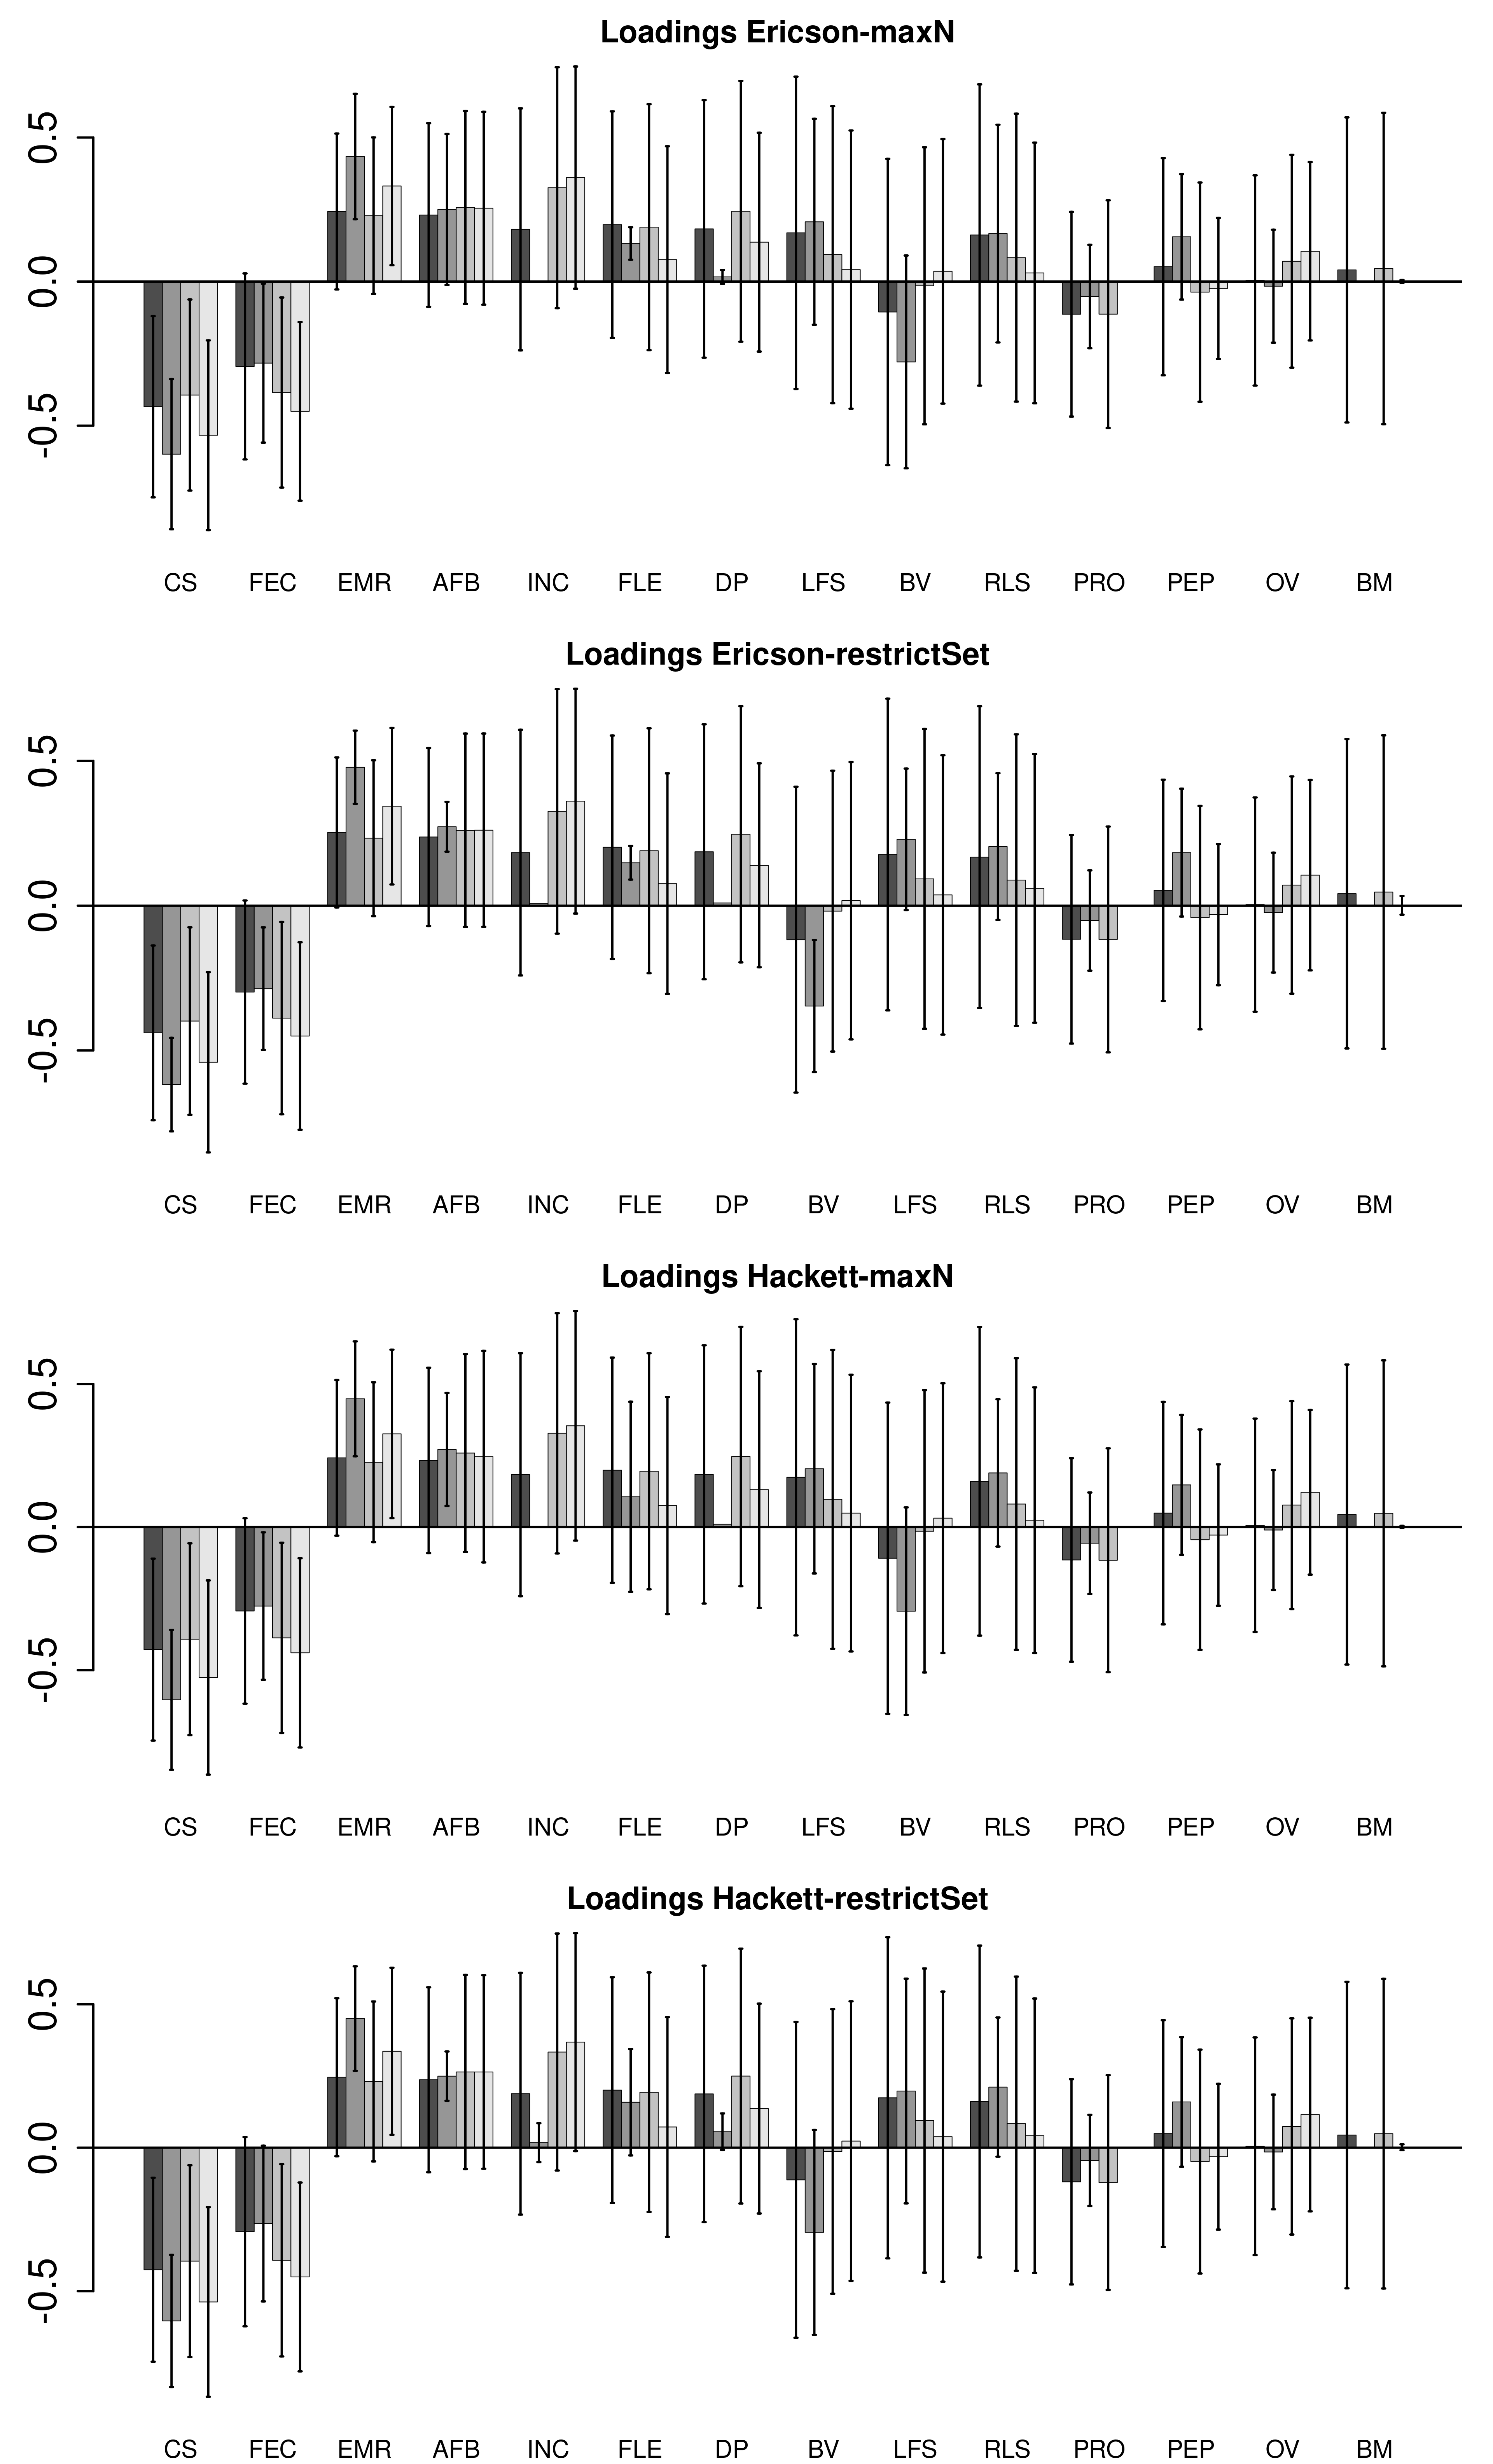
\includegraphics[width=.8\textwidth]{./Figures/Appendix2_1/FS loadings plots-ALL.png}
\caption[LHT loadings of the FS axes]{
Mean $\pm$ standard deviation AIC weighted loadings of the traits for the
fast-slow axes based on models predicting generation time or elasticity to
fecundity for all trait combination PCs o using only the PCs with AIC
\textless{2} (best AIC). From darker to lighter color: FSe, FSe best AIC, FSgt
and FSgt best AIC.}
\label{fig:figApp2.1}
\end{figure}

\begin{figure}[ht!]
\centering
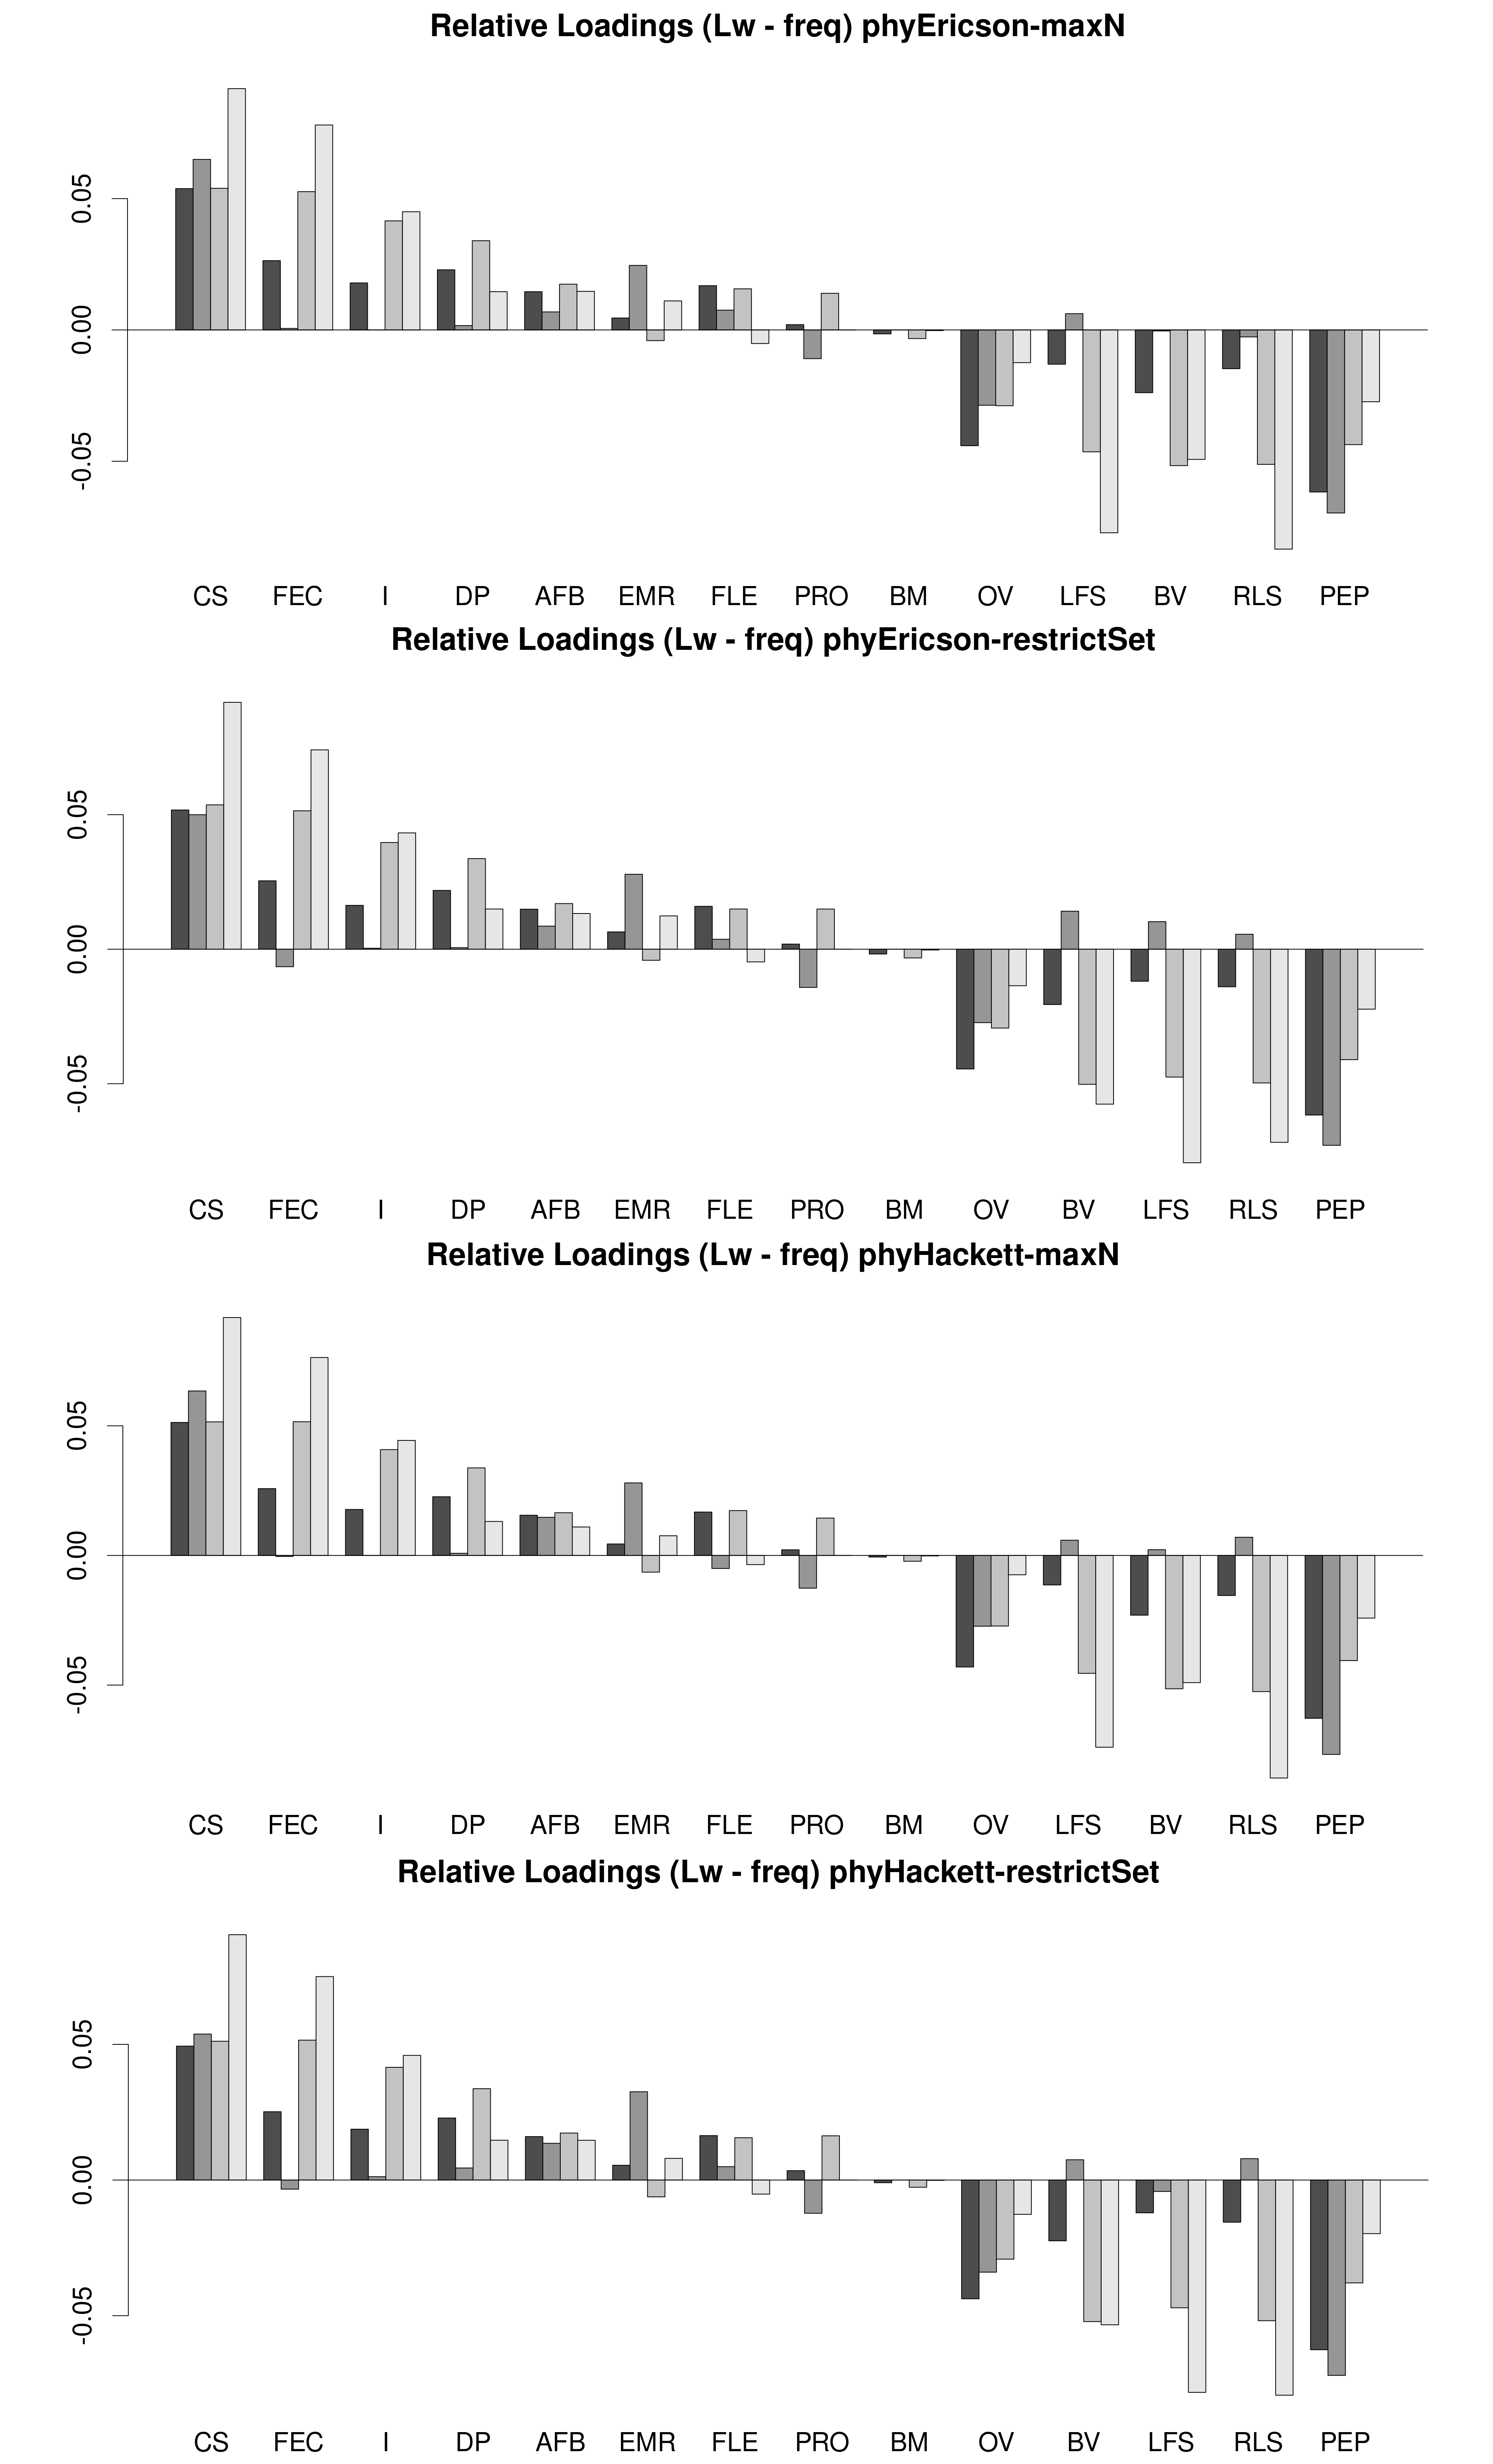
\includegraphics[width=.8\textwidth]{./Figures/Appendix2_1/FS relWeights plots-ALL.png}
\caption[LHT relative importance of the FS axes]{
Relative weight of the life history traits in the fast-slow continuum. Values
range from -1 to 1, where negative values means that the absolute value of the
trait loadings are lower than expected by the frequency of the trait and
positive values for traits with higher loadings than expected by the frequency
of the trait in the selected PPCAs (see main text for details). The loadings and
frequencies come from selected PCs that better predict elasticities to the
fecundity (FSe) or generation time (FSgt), weighted by the AIC based weight
of the models taking all or only the models with $\Delta AIC < 2$ (best AIC).
From darker to lighter color: FSe, FSe best AIC, FSgt and FSgt best AIC.}
\label{fig:figApp2.2}
\end{figure}

\begin{figure}[ht!]
\centering
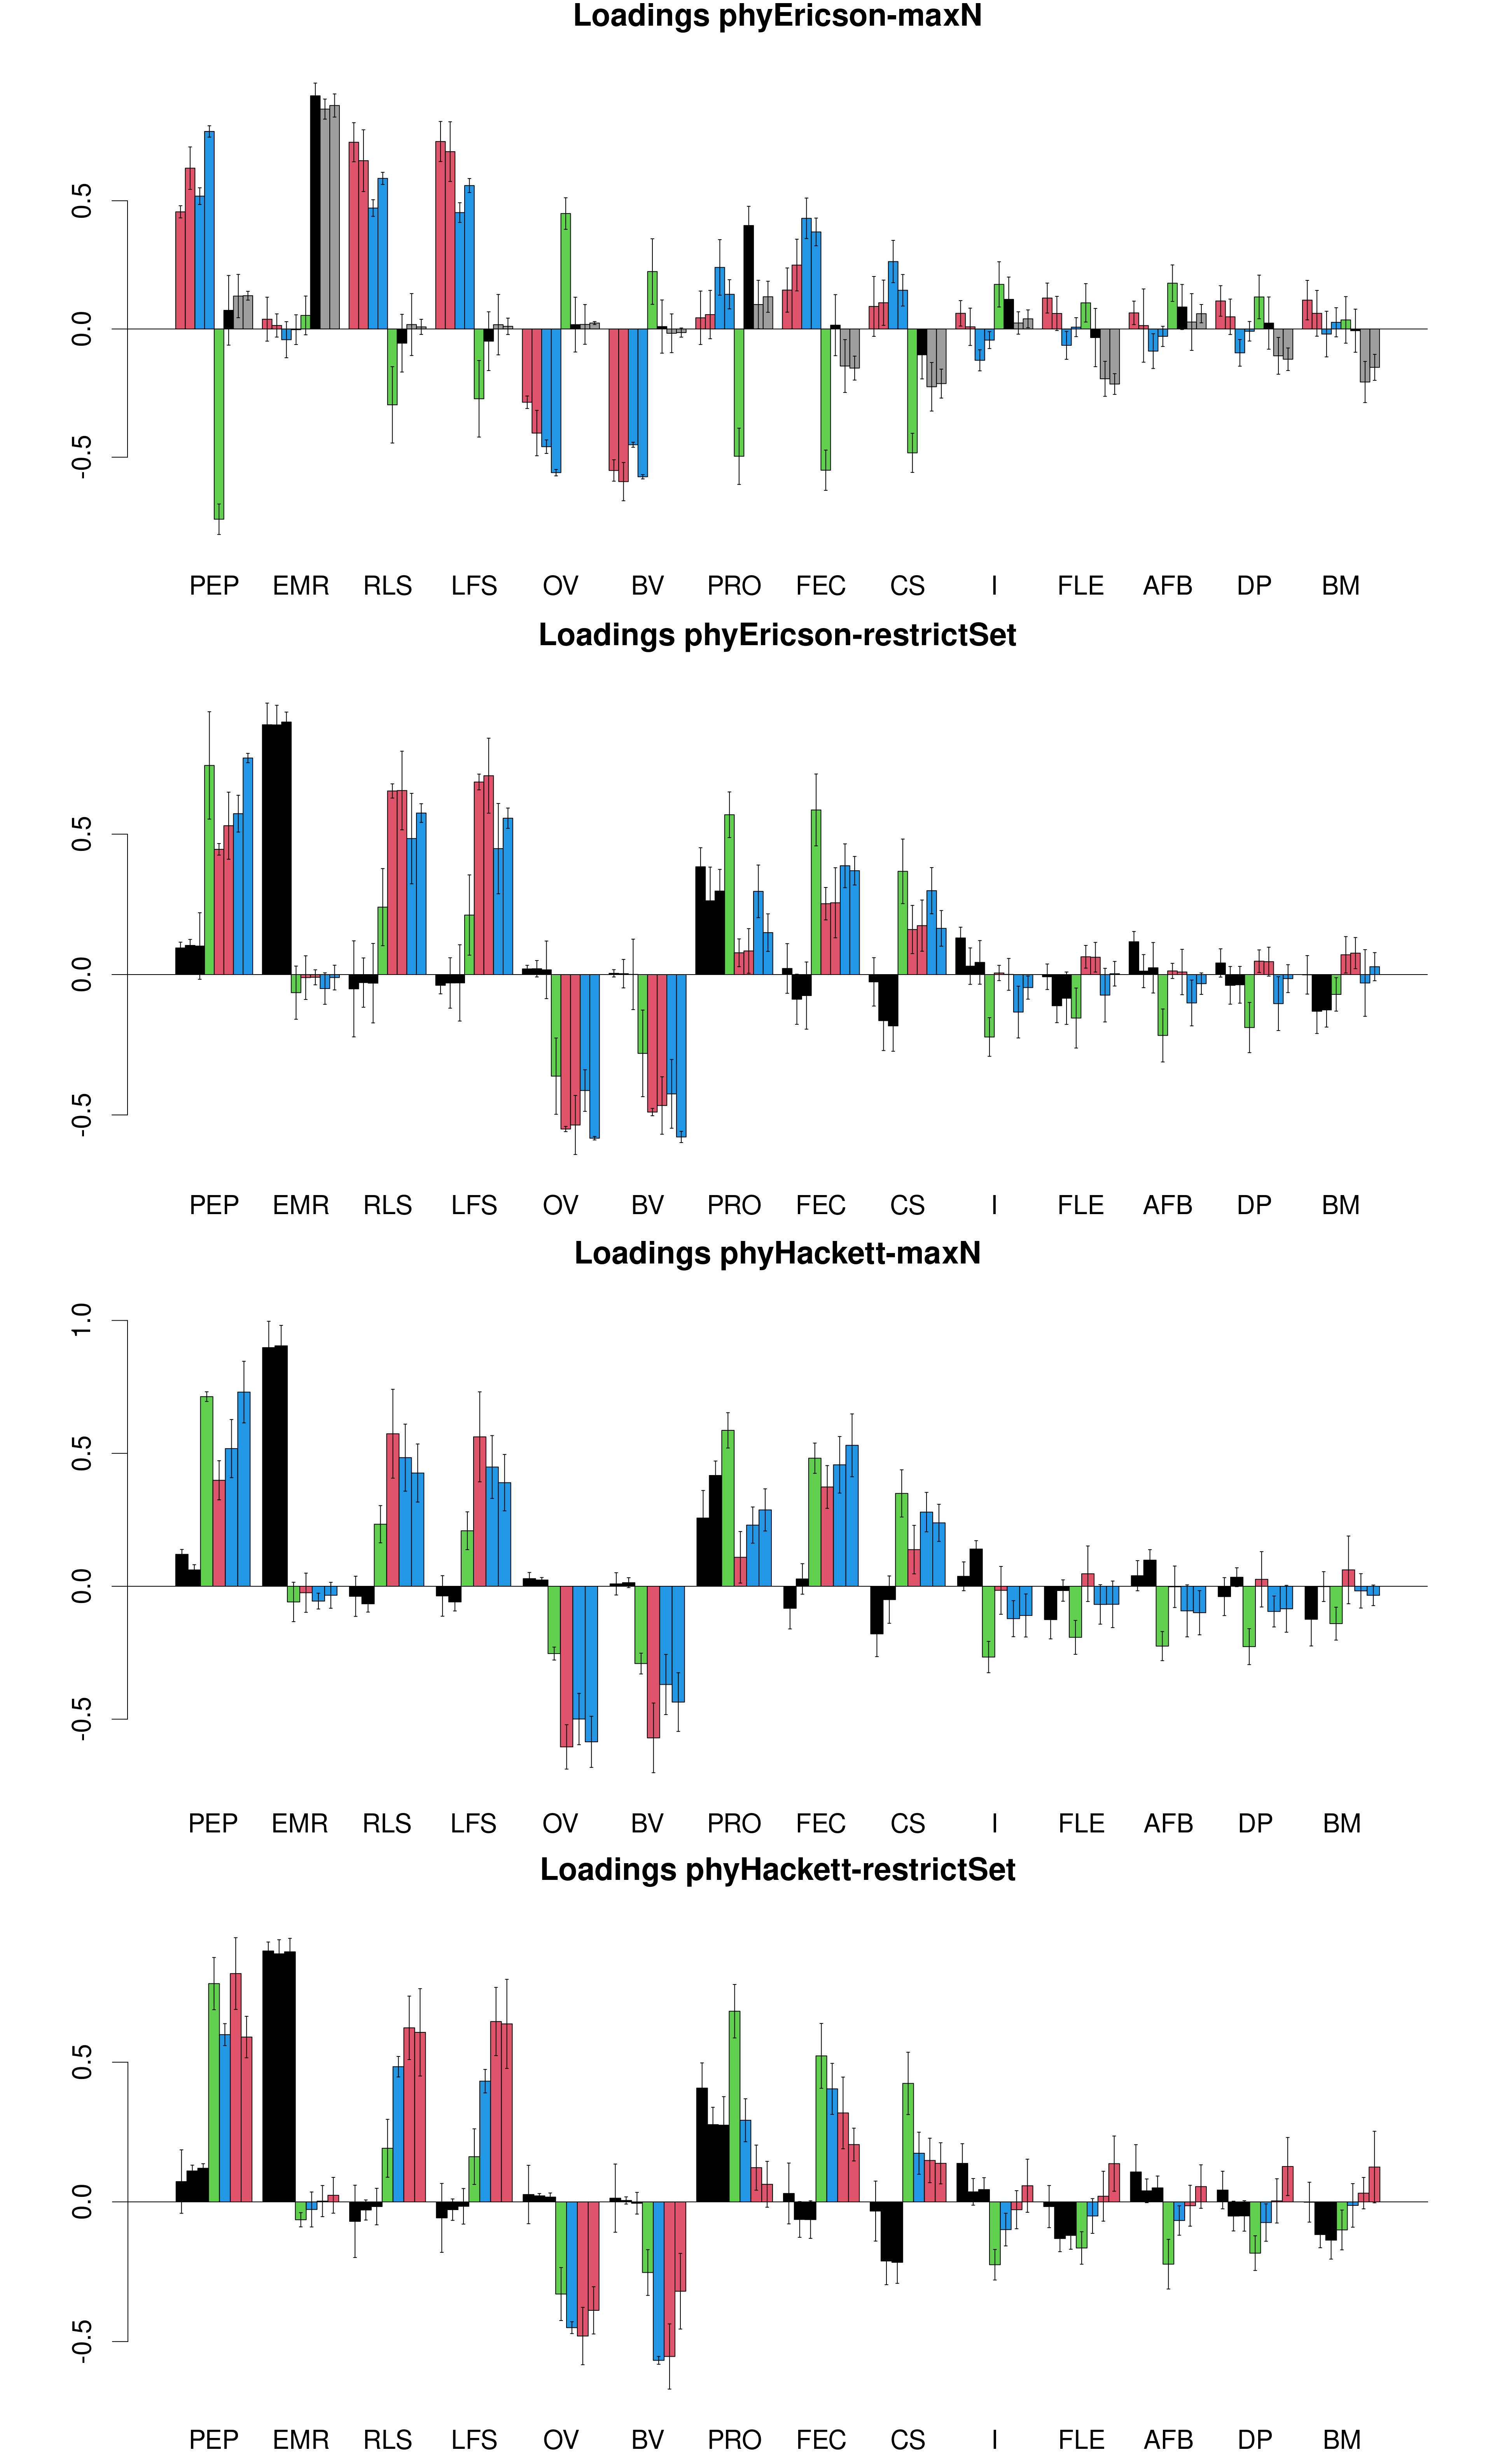
\includegraphics[width=.8\textwidth]{./Figures/Appendix2_1/2nd loadings plots-ALL.png}
\caption[LHT loadings of the secondary axes]{
Mean $\pm$ standard deviation of the loadings of the traits for clusters of
similar significant PCs (Eigenvalue \textgreater{1}) not selected for the
fast-slow axes. Groups follow the same order and colors than figure
\ref{fig:figApp2.5}.}
\label{fig:figApp2.3}
\end{figure}

\begin{figure}[ht!]
\centering
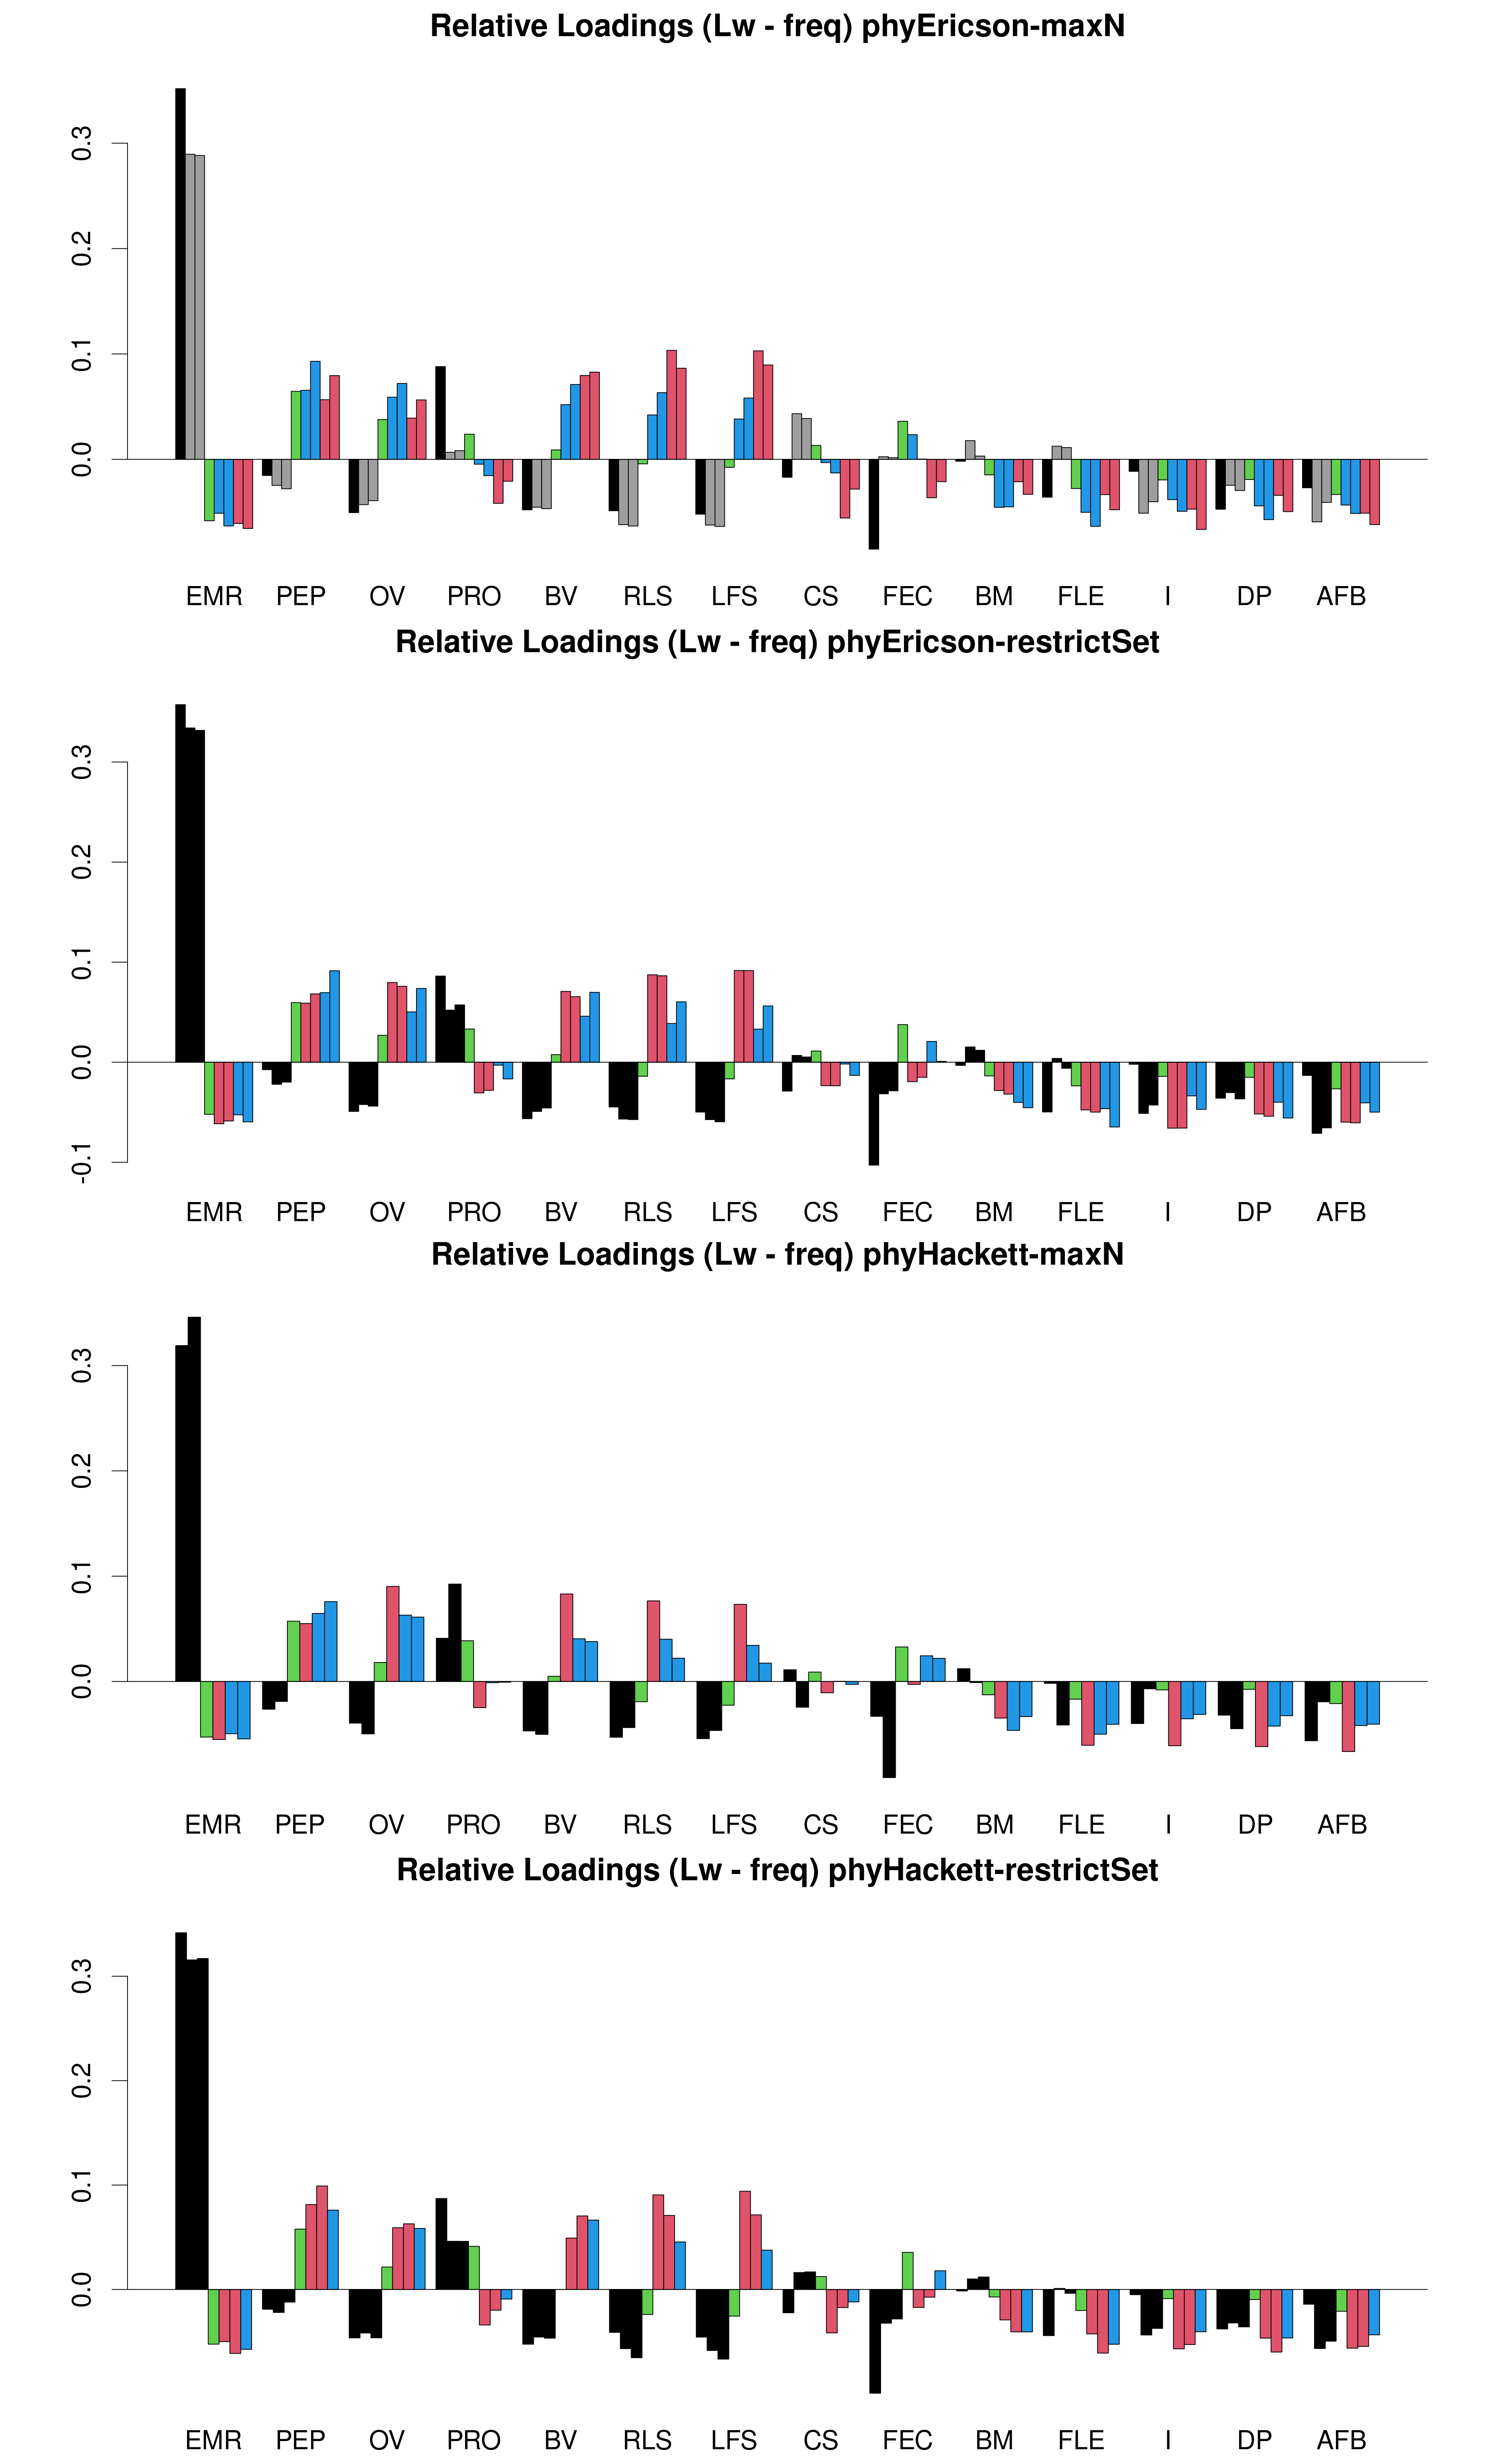
\includegraphics[width=.8\textwidth]{./Figures/Appendix2_1/2nd relWeights plots-ALL.png}
\caption[LHT relative importance of the secondary axes]{
Relative weights of the life history traits for each axes described in the
table \ref{tab:tabApp2.4}. Values range from -1 to 1, where negative values
means that the absolute value of the trait loadings are lower than expected by
the frequency of the trait and positive values for traits with higher loadings
than expected by the frequency of the trait in the selected PPCAs (see main
text for details). Groups follow the same order and colors as figure
\ref{fig:figApp2.5}.}
\label{fig:figApp2.4}
\end{figure}

\begin{figure}[ht!]
\centering
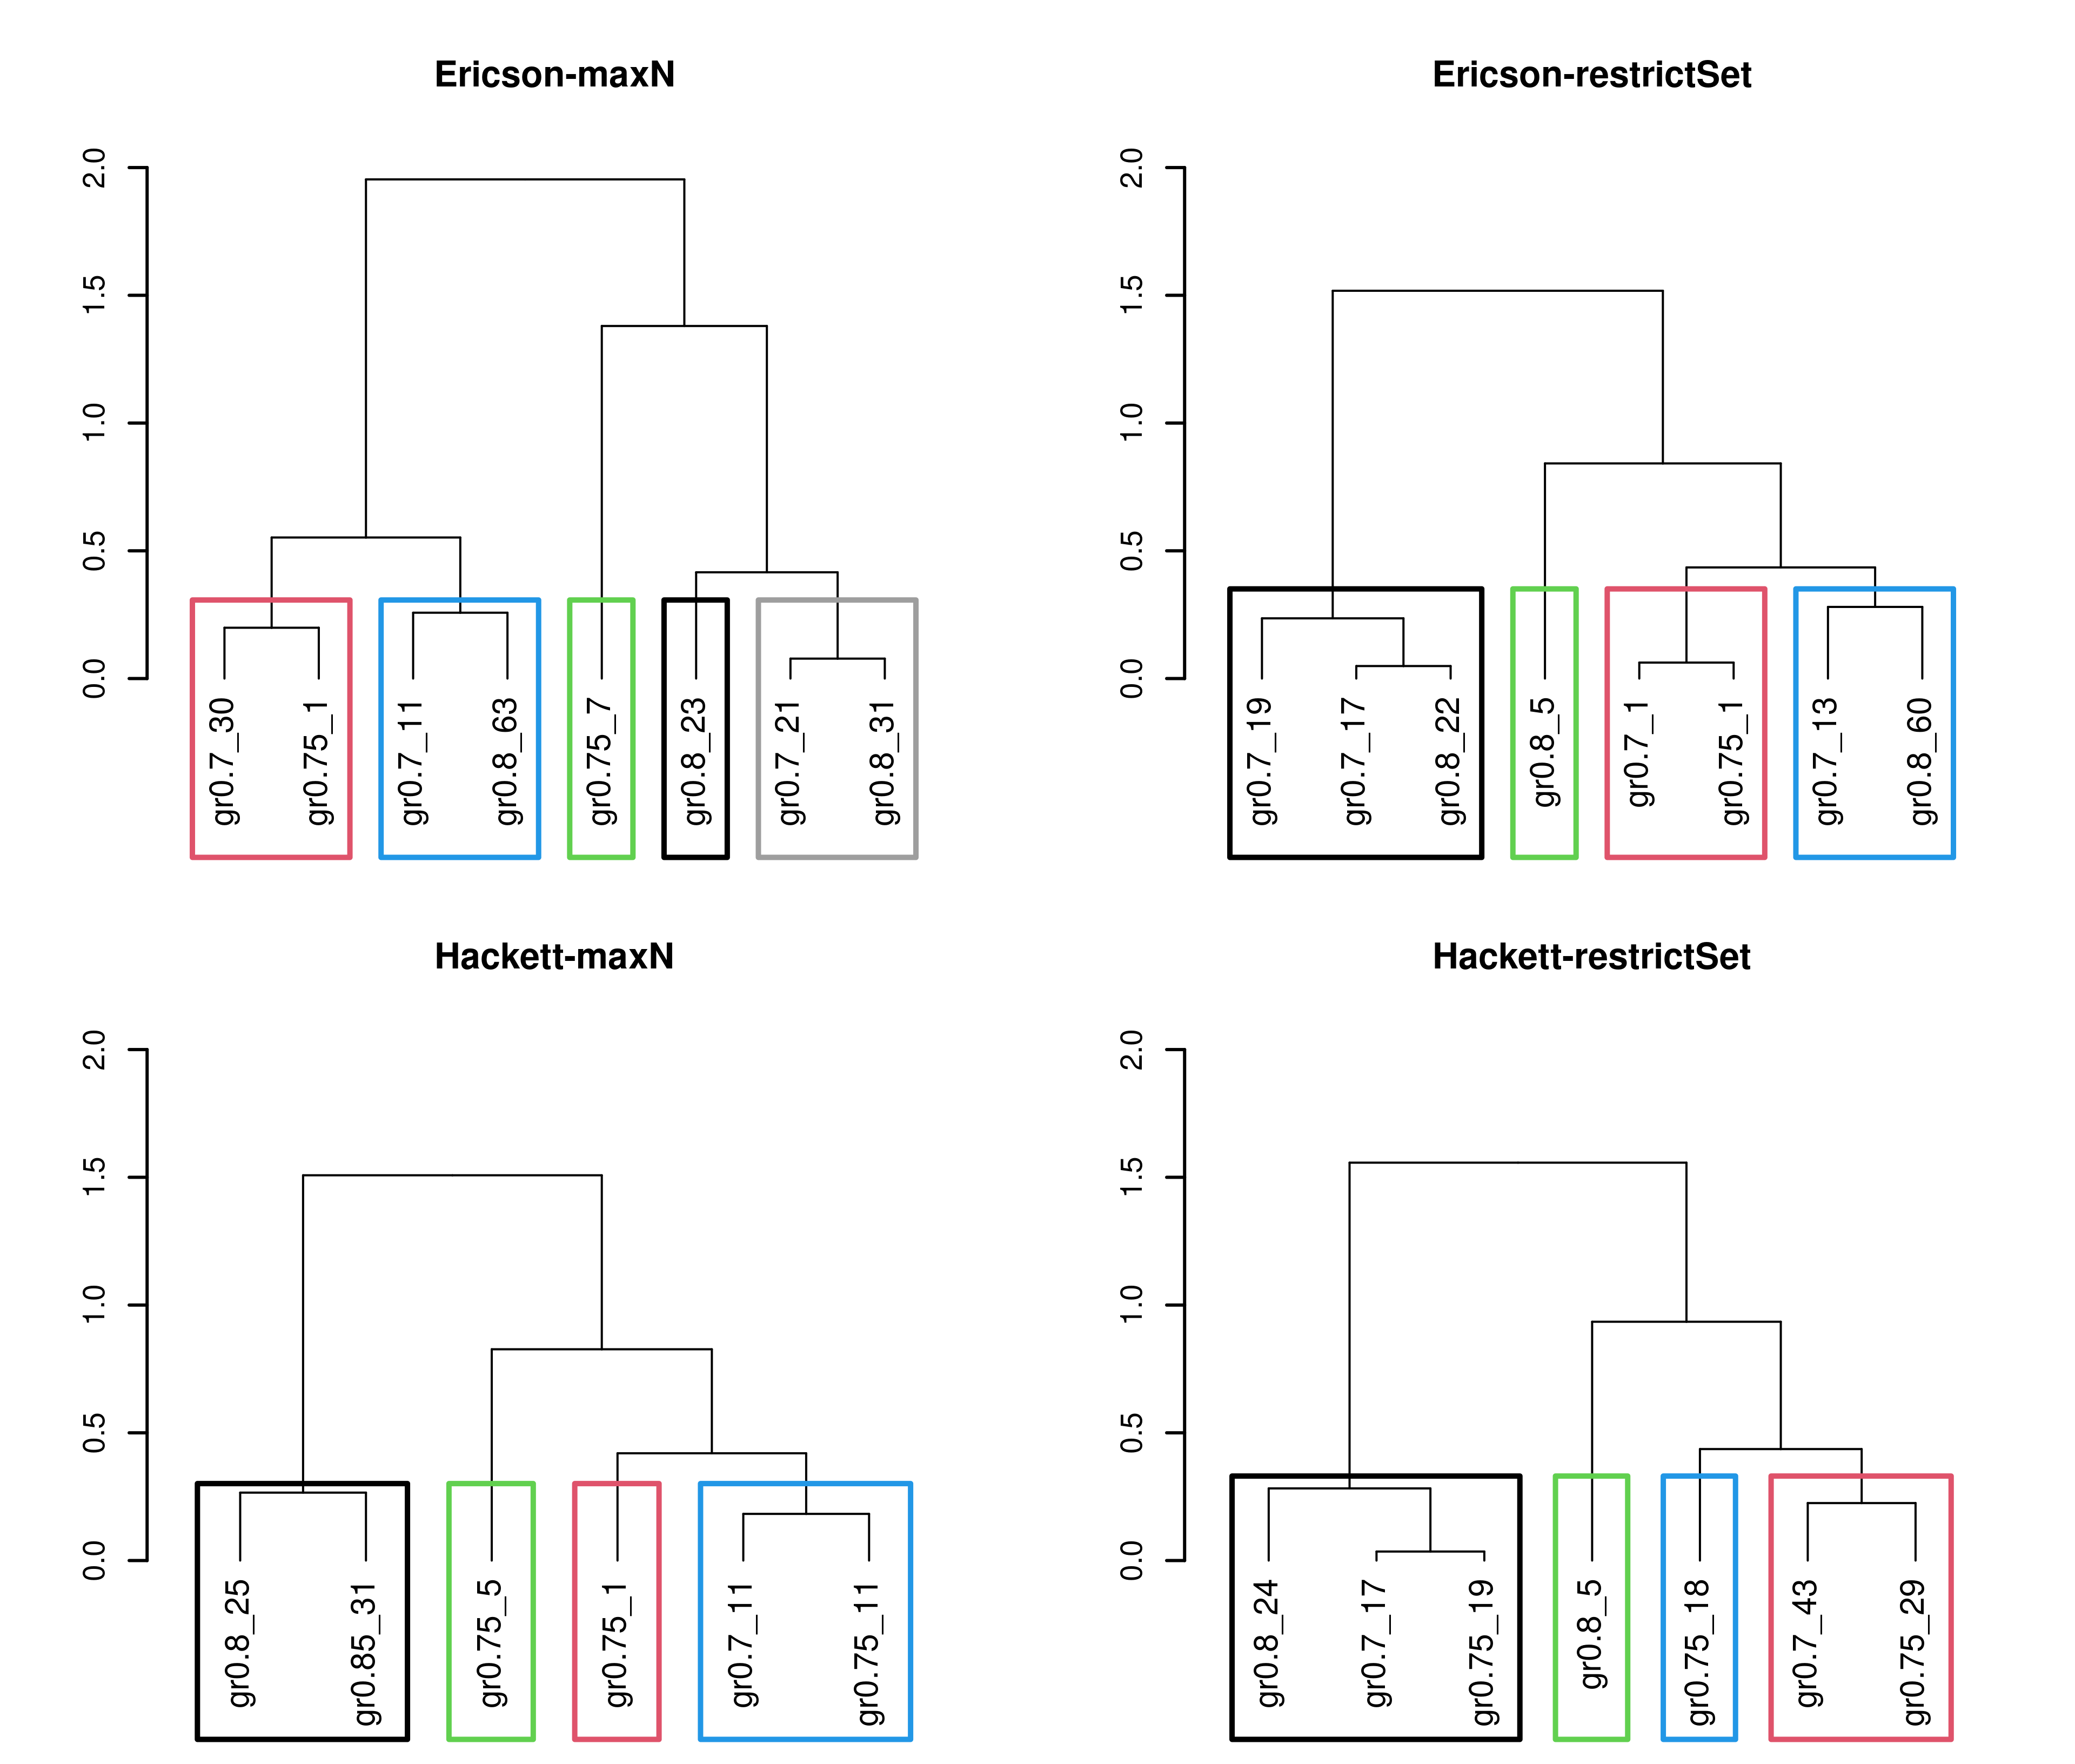
\includegraphics[width=.8\textwidth]{./Figures/Appendix2_1/2nd axes trees-1.png}
\caption[Cluster dendogram of the secondary axes]{
Dendogram of the distance among clusters of similar significant PCs (Eigenvalue
\textgreater{1}) not selected for the fast-slow axes. Each group contains PCs
with scores correlation greater than the correlation specified in the group name
(e.g. gr0.8 means correlation \textgreater{0.8}). Boxes include clusters with a
correlation among averaged loadings \textgreater{0.95} and can be conceptualized
as a offspring quality-quantity trade-off in black and grey, lifelong
productivity in green and iteroparity in blue and red.}
\label{fig:figApp2.5}
\end{figure}


%************************************************
\chapter[Appendix 3.1: Chapter 3 - Model description and parameterization]{
Appendix 3.1: Chapter 3 - Model description and parameterization}
\label{ch:Appendix3.1}
%************************************************
\renewcommand{\thefigure}{A.3.1.\arabic{figure}}
\setcounter{figure}{0}

\renewcommand{\thetable}{A.3.1.\arabic{table}}
\setcounter{table}{0}

\section*{Description of the stochastic population model}\label{model-description}

At any temporal point in a given simulation run the population is described by a
cohort of juveniles, sub-adults at all stages, non-breeding adults (i.e. those
that skip breeding) and failed and successful adult breeders. Those individuals
may belong to one of the two habitats that typify our simulated scenario. Growth
from one stage to the next one, shift between habitats and the birth and
establishment of new individuals are all computed by stochastically drawing from
corresponding binomial distributions. See Figure \ref{fig:figApp3.2.1} for a graphic overview of
all possible state transitions and Table \ref{tab:tabApp3.1.1} for parameters definition.

\begin{enumerate}
  \item The first calculation, for a given temporal step $t$ and for each
habitat, is to calculate how many full adults will become non-breeders and how
many will be (successful or failed) breeders:
    \begin{equation*}
      A_{h,t}^{b} = Bin \left( {A}_{h,t} , {p}_{h}^{b} \right)
    \end{equation*}

  \item Then, we enter the breeding algorithm, which runs recursively $m$ times
within a loop. Within this loop only juvenile recruitment and survival, as well 
as habitat shift for successful and failed adult breeders are evaluated.
  \begin{enumerate}
    \item Within the loop, at the beginning of a given brooding event $i$, the
number of adults that breed successfully is decided for each habitat by randomly
drawing from a binomial distribution:
      \begin{equation*}
        A_{h,t}^{b_{s}} = Bin \left( {A}_{h,t}^{b} , 1 - {p}_{h}^{b_{f}} \right)
      \end{equation*}
    \item That, in turn, allows us to calculate the number of adults that fail 
to breed:
      \begin{equation*}
        A_{h,t}^{b_{f}} = A_{h,t}^{b} - A_{h,t}^{b_{s}}
      \end{equation*}
    \item Then, the number of juveniles that are bred and survive until the 
next year are updated at each loop step as:
      \begin{equation*}
        {J}_{h,t} = {J}_{h,t} + Bin \left( {A}_{h,t}^{{b}_{s}} \cdot q, {p}_{h, 
{S}_{j}} \right)
      \end{equation*}
    \item Next, after hatching has taken place, part of the successful or 
failed adult population may move between habitats. We model those actions by 
stochastically drawing from a binomial distribution the number of adults that 
change habitat:
      \begin{equation*}
{\Delta}_{1\rightarrow2}^{x} =Bin \left({A}_{1,t}^{x} , {p}_{1\rightarrow2}^
{x} \right)
      \end{equation*}
      \begin{equation*}
{\Delta}_{2\rightarrow1}^{x} =Bin \left({A}_{2,t}^{x} , {p}_{2\rightarrow1}^
{x} \right)
      \end{equation*}
Where, in this case, $x \in \{ {b}_{s} , {b}_{f} \}$.
    \item Then, the number of successful and failed breeders will be updated:
      \begin{equation*}
{A}_{1,t}^{x} = {A}_{1,t}^{x} - {\Delta}_{1\rightarrow2}^{x} +
{\Delta}_{2\rightarrow1}^{x}
      \end{equation*}
      \begin{equation*}
{A}_{2,t}^{x} = {A}_{2,t}^{x} - {\Delta}_{2\rightarrow1}^{x} +
{\Delta}_{1\rightarrow2}^{x}
      \end{equation*}
    And thus, with the new calculation:
      \begin{equation*}
{A}_{1,t}^{b} = {A}_{1,t}^{{b}_{s}} + {A}_{1,t}^{{b}_{f}}
    \end{equation*}
    \begin{equation*}
{A}_{2,t}^{b} = {A}_{2,t}^{{b}_{s}} + {A}_{2,t}^{{b}_{f}}
      \end{equation*}
    Then the algorithm goes back to point a) above $m$ times, after which it 
jumps from e) above to point 3 just below.
  \end{enumerate}
  \item When the simulation includes sub-adults (i.e. age of first reproduction 
\textgreater{1}), we must account for the fact that they may also move between habitats:
    \begin{equation*}
{\Delta}_{1\rightarrow2}^{r} =Bin \left({S}_{1,t}^{r} , {p}_{1\rightarrow2}^{r}
\right)
    \end{equation*}
    \begin{equation*}
{\Delta}_{1\rightarrow2}^{r} =Bin \left({S}_{2,t}^{r} , {p}_{2\rightarrow1}^{r}
\right)
    \end{equation*}
  \item Moreover, sub-adults are also affected by survival, which is modeled by 
stochastically drawing from a binomial distribution:
    \begin{equation*}
{S}_{1,t+1}^{r} =Bin \left({S}_{1,t+1}^{r} - {\Delta}_{1\rightarrow2}^{r} +
{\Delta}_{2\rightarrow1}^{r} , {p}_{1, {S}_{sa}} \right)
    \end{equation*}
    \begin{equation*}
{S}_{2,t+1}^{r} =Bin \left({S}_{2,t+1}^{r} - {\Delta}_{2\rightarrow1}^{r} +
{\Delta}_{1\rightarrow2}^{r} , {p}_{{2,S}_{sa}} \right)
    \end{equation*}
  \item Then, we also allow non-breeders to change habitats by stochastically 
drawing from a binomial distribution:
    \begin{equation*}
{\Delta}_{1\rightarrow2,t}^{nb} = Bin \left({A}_{1,t}^{nb},
{p}_{1\rightarrow2}^{nb} \right)
    \end{equation*}
    \begin{equation*}
{\Delta}_{2\rightarrow1,t}^{nb} = Bin \left({A}_{1,t}^{nb},
{p}_{2\rightarrow1}^{nb} \right)
    \end{equation*}
  \item Consequently, the population at $t+1$ of those non-breeding adults must 
be updated as follows:
    \begin{equation*}
{A}_{1,t+1}^{nb} = {A}_{1,t}^{nb} - {\Delta}_{1\rightarrow2}^{nb} +
{\Delta}_{2\rightarrow1}^{nb}
    \end{equation*}
    \begin{equation*}
{A}_{2,t+1}^{nb} = {A}_{2,t}^{nb} - {\Delta}_{2\rightarrow1}^{nb} +
{\Delta}_{1\rightarrow2}^{nb}
    \end{equation*}
  \item Next, we account for survival probability of all types of adults:
    \begin{equation*}
{A}_{h,t+1}^{x} =Bin \left({A}_{h,t+1}^{x} , {p}_{h, {S}_{x}} \right)
    \end{equation*}
  where, in this case, $x \in \{ {b}_{s}, {b}_{f}, nb \}$. Values
${A}_{h,t+1}^{x}$ inside the binomial correspond to those at the end of the
breeding loop when $x=b_{s}$ or $x=b_{f}$.
  \item Total adult population is then:
    \begin{equation*}
{A}_{h,t+1} = \sum_{x \in \{ {b}_{s}, {b}_{f}, nb \}} {{A}_{h,t+1}^{x}}
    \end{equation*}
  \item Finally, populations are updated simply by moving up one stage and 
juveniles become adults or sub-adults according to the age of first 
reproduction.
\end{enumerate}


\section*{Exploration of the parameter space}\label{model-exploration}

The range of demographic parameters comes from empirical data from birds. With 
the chosen parameters we estimated juvenile survival $p_{1,s}$ for a given 
deterministic growth rate $\lambda$ corresponding to the Leslie matrix model by
solving the Euler-Lotka equation:

\begin{equation*}
{p}_{1, {S}_{j}} = \frac {{{p}_{1, {S}_{sa}}} ^ {1-AFR} \left({\lambda}^{1+AFR}
- {p}_{1, {S}_{b}} \cdot {\lambda} ^ {AFR} \right)} {q \cdot \lambda}
\end{equation*}

where $AFR$ is the age at first reproduction and other notation follows Table
\ref{tab:tabApp3.1.1}. Once demographic parameters in habitat 1 are defined we
modify the habitat 2 parameters according to the different scenarios. In
Scenario 1, the parameters in habitat 2 are the same than in habitat 1. In
Scenario 2 we increase adult and subadult mortality $n$ times (1.5 in Scenario
2.1 and 2 in Scenario 2.2). To increase $p$ probabilities $n$ times we apply
$p^{n}$ and therefore, adult survival in habitat 2 is:
\begin{equation*}
{p}_{2, {S}_{b}} =1- {\left(1- {p}_{1, {S}_{b}} \right)}^{{1} / {n}}
\end{equation*}

For Scenario 3 we apply the increase in breeding fail as follows:

\begin{equation*}
{p}_{2}^{{b}_{f}} =1- {\left(1- {p}_{1}^{{b}_{f}} \right)}^{{1} / {n}}
\end{equation*}

\clearpage


\begin{table}
\caption[Notation]{Notation followed to describe the stochastic population model.}\label{tab:tabApp3.1.1}
\begin{tabular}[b]{@{}p{1.5cm}p{13cm}@{}}
\toprule
\textbf{Symbol} & \textbf{Definition}                                                                                                                                                                                             \\ \midrule
$q$   & Number of offsprings per brood in habitat $h$                                                                                                                                                                             \\
$m$   & Number of broods per year                                                                                                                                                                                                 \\
${n}_{Sa}$        & Number of sub-adult stages                                                                                                                                                                                    \\
$x$   & Labels $x$ may take the values $j, sa, b, nb, b_{s}, b_{f}$, where these values refer to juveniles, subadults, adults (i.e. sum of all types), non-breeding adults, successful breeders and failed breeders, respectively \\
$h$   & Index for habitat type, $h=\{1, 2\}$                                                                                                                                                                                      \\
$r$   & Label for subadult stage, $r \in \{r_{1} \cdots r_{n_{Sa}}\}$                                                                                                                                                             \\
$t$   & Subindex for time steps, measured in years, $t= \{1 \cdots 50\}$                                                                                                                                                          \\
${p}_{h}^{b}$     & Probability for an individual to become a breeder (successful or not) in habitat $h$                                                                                                                          \\
${p}_{h}^{b_{f}}$ & Probability for a possible breeder individual to be a failed breeder in habitat $h$                                                                                                                           \\
${p}_{h,S_{x}}$   & Probability of survival in habitat $h$ for individuals $x$                                                                                                                                                    \\
\noalign{\bigskip}
${p}_{1\rightarrow2}^{x}$ \\ ${p}_{2\rightarrow1}^{x}$ & Probability for an adult to move from habitat type 1 to 2, or vice versa                                                                                                 \\
\noalign{\bigskip}
${p}_{1\rightarrow2}^{r}$ \\ ${p}_{2\rightarrow1}^{r}$ & Probability for a stage-r subadult to move from habitat type 1 to 2, or vice versa                                                                                       \\
\noalign{\smallskip}
${J}_{h,t}$       & Number of juveniles that have born in habitat $h$ at time step $t$                                                                                                                                            \\
${S}_{h,t}^{r}$   & Number of stage-$r$ subadults in habitat $h$ in year $t$                                                                                                                                                      \\
${A}_{h,t}$       & Total number of adults in habitat $h$ at time $t$                                                                                                                                                             \\
${A}_{h,t}^{x}$   & Number of adults of type $x$ in habitat $h$ at time step $t$                                                                                                                                                  \\
\noalign{\bigskip}
${\Delta}_{1\rightarrow2}^{x}$ \\ ${\Delta}_{2\rightarrow1}^{x}$   & Number of adults that will move from habitat type 1 to habitat 2, or viceversa                                                                               \\
\noalign{\smallskip}
${\Delta}_{1\rightarrow2}^{r}$ \\ ${\Delta}_{2\rightarrow1}^{r}$   & Number of sub-adults that will move from habitat type 1 to habitat 2, or viceversa                                                                           \\ \bottomrule
\end{tabular}
\end{table}

%************************************************
\chapter[Appendix 3.2: Chapter 3 - Supplementary Figures]{Appendix 3.2: Chapter 3 - Supplementary figures}\label{ch:Appendix3.2}
%************************************************
\renewcommand{\thefigure}{A.3.2.\arabic{figure}}
\setcounter{figure}{0}

\renewcommand{\thetable}{A.3.2.\arabic{table}}
\setcounter{table}{0}

\begin{figure}[ht!]
\centering
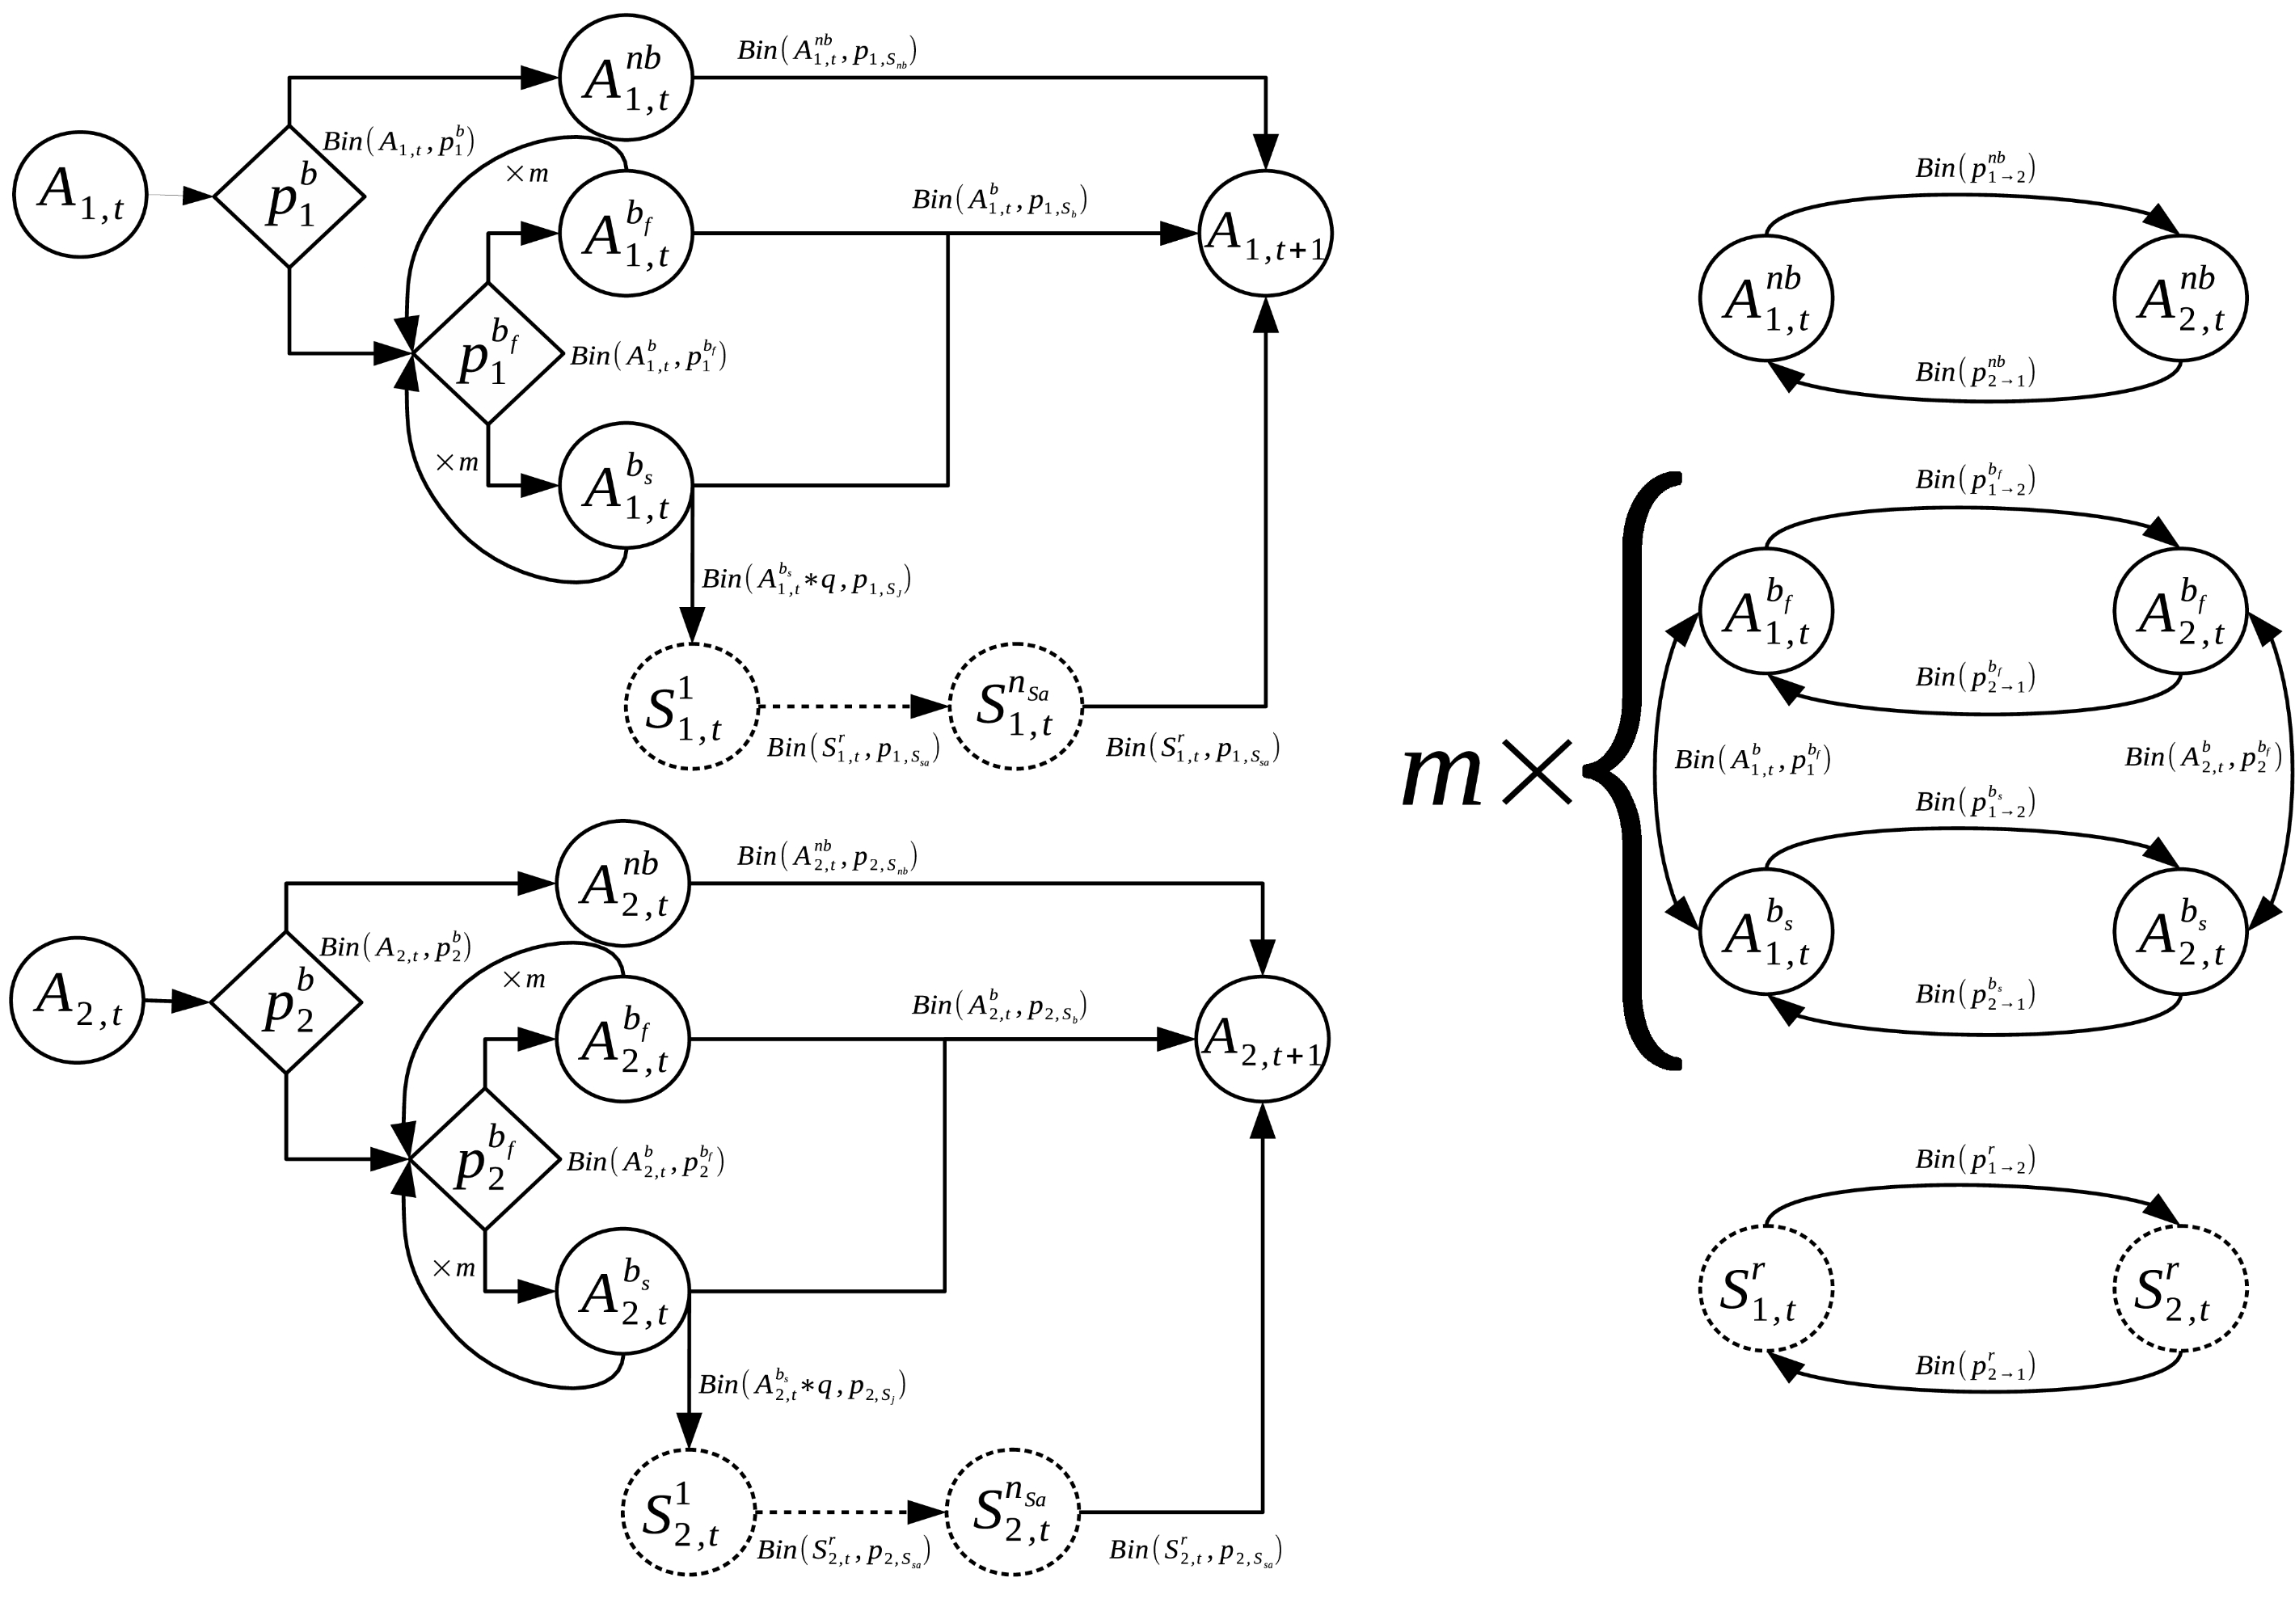
\includegraphics[width=\textwidth]{./Figures/Appendix3_2/Fig_1.jpg}
\caption[Flowchart of the model]{
Flowchart of the stochastic simulation model. Notation is the same as in Table
\ref{tab:tabApp3.1.1} above.}
\label{fig:figApp3.2.1}
\end{figure}

\begin{figure}
\centering
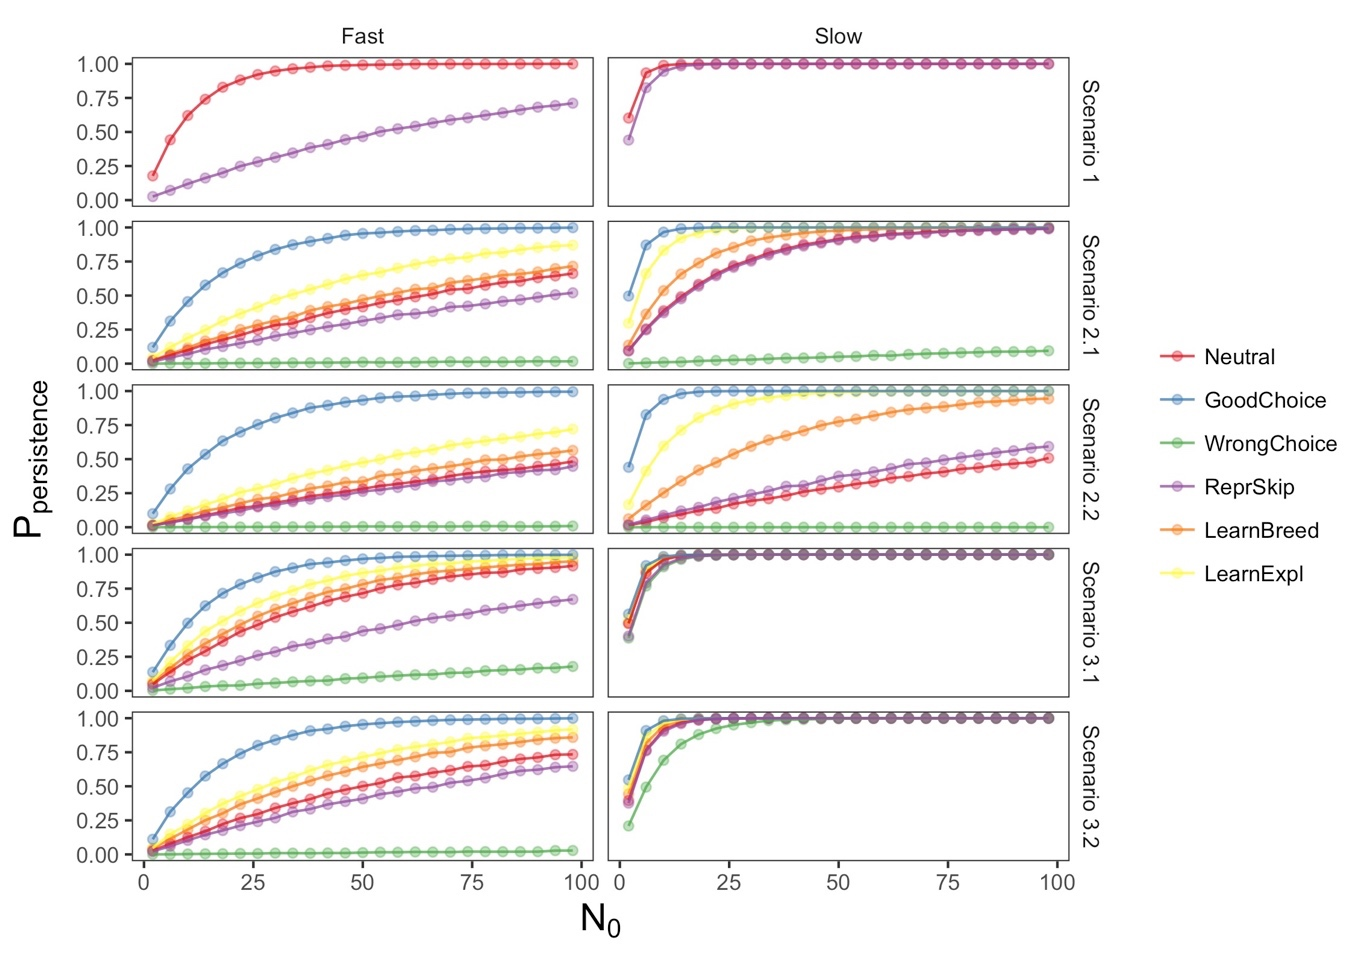
\includegraphics[width=\textwidth]{./Figures/Appendix3_2/Fig_2.jpg}
\caption[Persistence with strong behavioural responses]{
Simulations of probability of population persistence as a function
of behavioural responses for different initial population sizes according to
different life histories (fast and slow). See figure \ref{fig:fig3.1} for
details. In this case we shown the results for simulations with strong
behavioural responses.}
\label{fig:figApp3.2.2}
\end{figure}

\begin{figure}
\centering
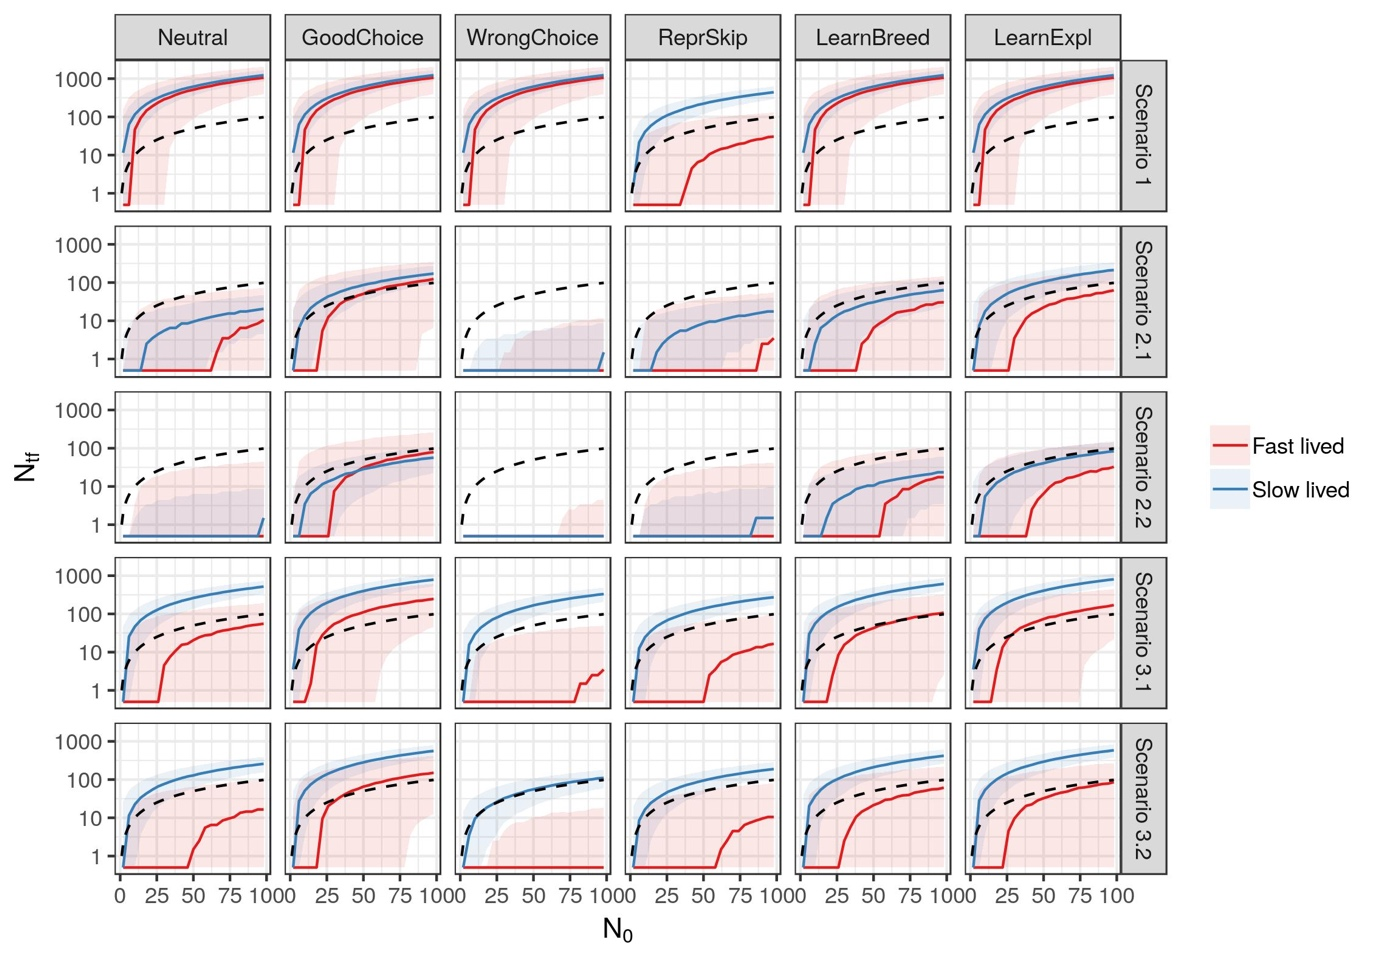
\includegraphics[width=\textwidth]{./Figures/Appendix3_2/Fig_3.jpg}
\caption[Effects on $N_{tf}$]{
Final population size ($N_{tf}$, median and 95\% confidence interval
of the 10000 replicates) of the simulations shown in figure \ref{fig:fig3.1}.
Black dashed lines show the initial population size.}
\label{fig:figApp3.2.3}
\end{figure}

\begin{figure}
\centering
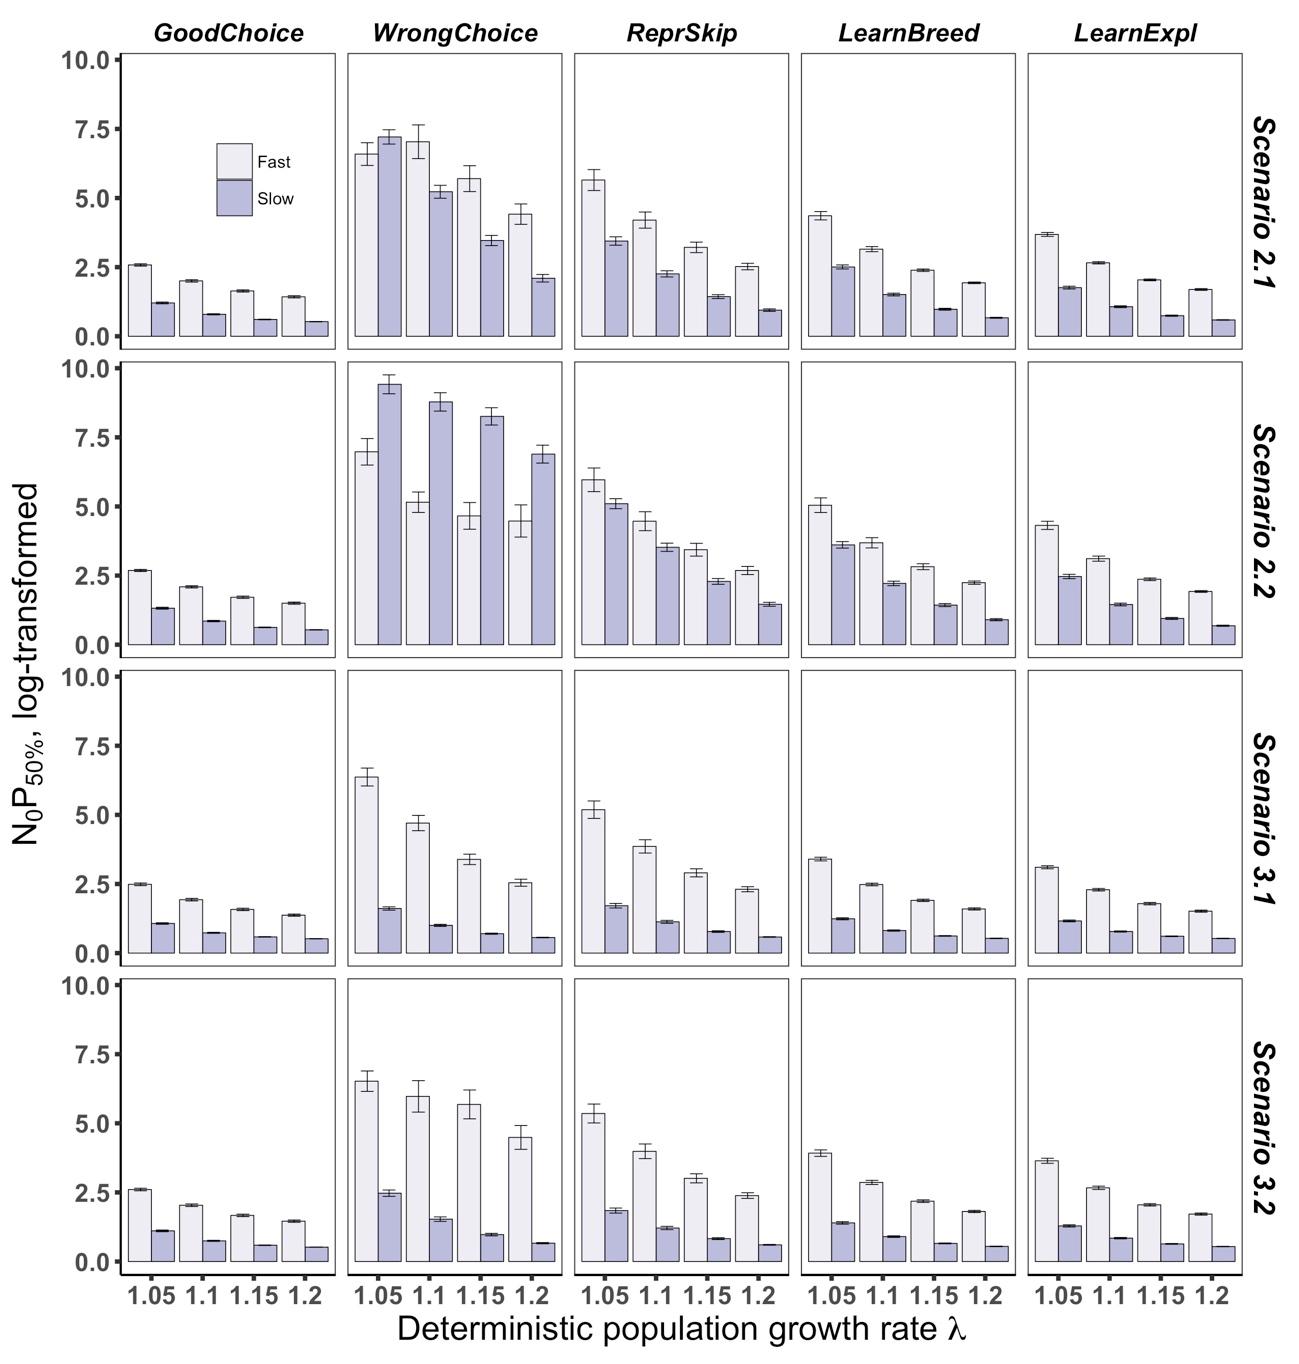
\includegraphics[width=\textwidth]{./Figures/Appendix3_2/Fig_4.jpg}
\caption[Effects on $N_{0}P_{50\%}$ with strong behavioural responses]{
Effects of behavioural responses on population persistence in novel
environments as a function of the position of the animal along the fast-slow
continuum. Population persistence is estimated as $N_{0}P_{50\%}$ and
behavioural responses are strong. The position of the animal along the fast-slow
continuum is assessed as the relative sensitivity (i.e. elasticity) of
population growth to changes in fecundity, with slow-lived strategies exhibiting
low elasticities and fast-lived strategies exhibiting high elasticities. For
details on abbreviation, see figure \ref{fig:fig3.1}.}
\label{fig:figApp3.2.4}
\end{figure}

\begin{figure}
\centering
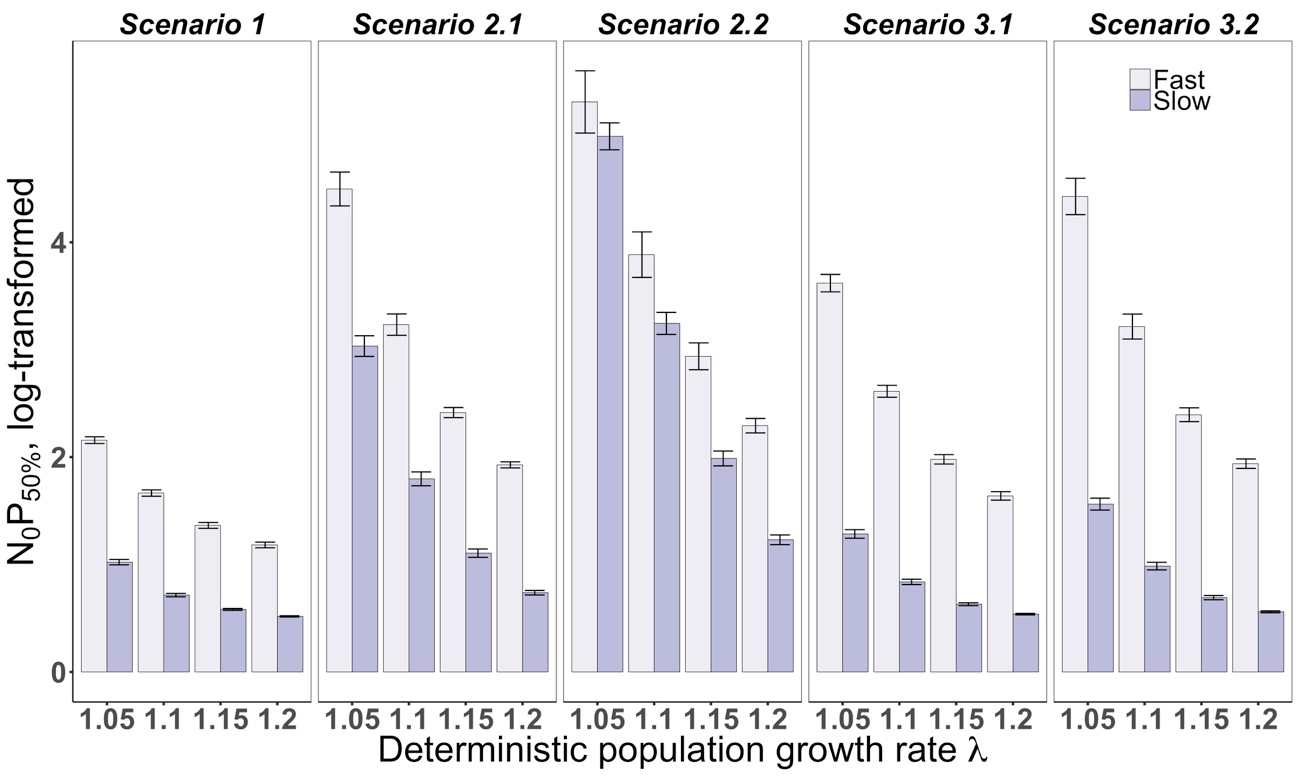
\includegraphics[width=\textwidth]{./Figures/Appendix3_2/Fig_5.jpg}
\caption[Effects on $N_{0}P_{50\%}$ with neutral behaviour]{
Population persistence in novel environments as a function of the
position of the animal along the fast-slow continuum for different scenarios and
neutral behaviour. Population persistence is estimated as $N_{0}P_{50\%}$.}
\label{fig:figApp3.2.5}
\end{figure}

\begin{figure}
\centering
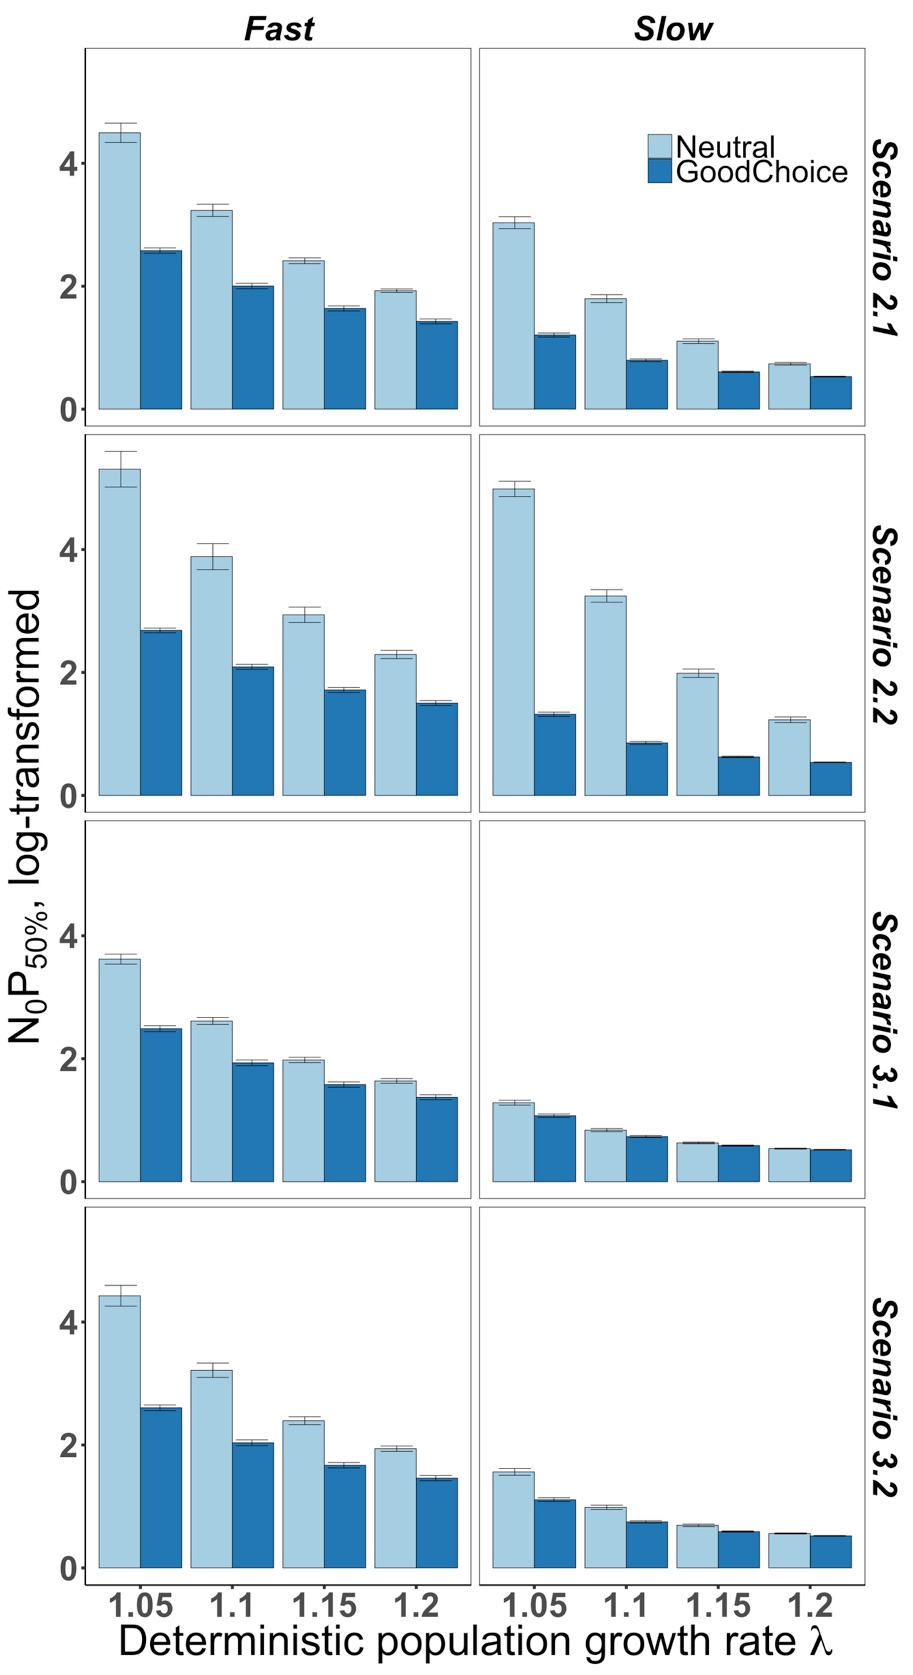
\includegraphics[height=.75\textheight]{./Figures/Appendix3_2/Fig_6.jpg}
\caption[Effects of \textit{GoodChoice} on $N_{0}P_{50\%}$]{
Influence of habitat matching choice on population persistence in novel
environments as a function of the position of the species along the fast-slow
continuum. Benefits and costs of the behaviour under different environmental
scenarios are reflected in differences in $N_{0}P_{50\%}$ between simulations
where individuals’ behaviour is either considered neutral or to reflect an
innate preference for the high-quality habitat.}
\label{fig:figApp3.2.6}
\end{figure}

\begin{figure}
\centering
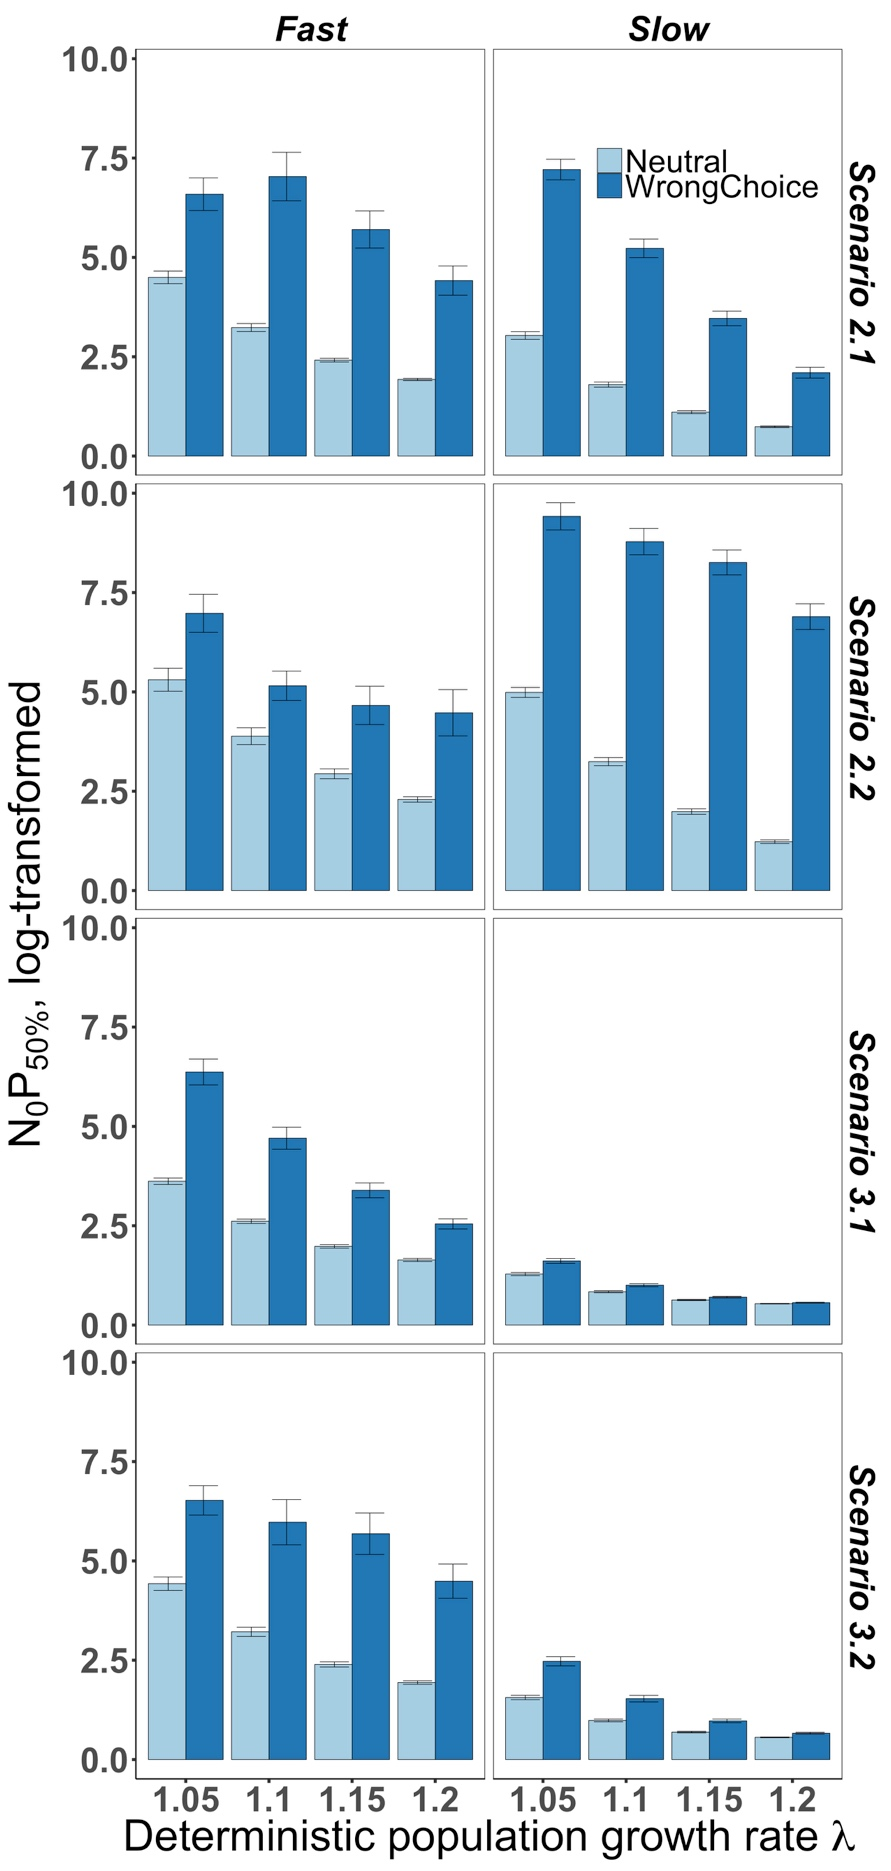
\includegraphics[height=.75\textheight]{./Figures/Appendix3_2/Fig_7.jpg}
\caption[Effects of \textit{WrongChoice} on $N_{0}P_{50\%}$]{
Influence of an inappropriate habitat matching choice on population persistence
in novel environments as a function of the position of the species along the
fast-slow continuum. Benefits and costs of the behaviour under different
environmental scenarios are reflected in differences in $N_{0}P_{50\%}$ between
simulations where individuals’ behaviour is either considered neutral or to
reflect an innate preference for the low-quality habitat.}
\label{fig:figApp3.2.7}
\end{figure}

\begin{figure}
\centering
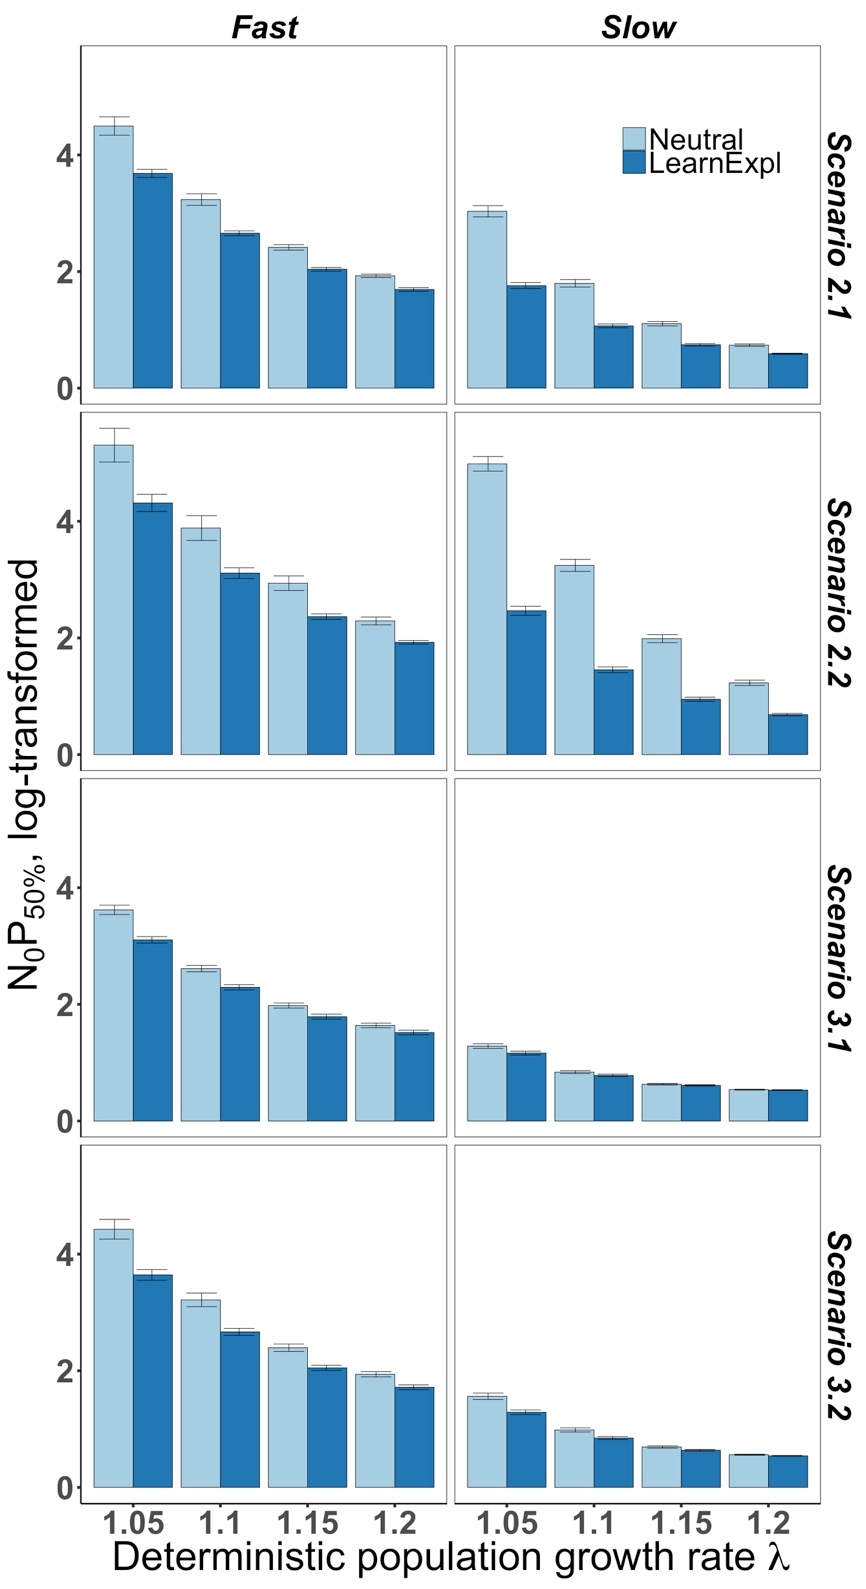
\includegraphics[height=.75\textheight]{./Figures/Appendix3_2/Fig_8.jpg}
\caption[Effects of \textit{LearnExpl} on $N_{0}P_{50\%}$]{
Influence of learning through exploration on population persistence in novel
environments as a function of the position of the species along the fast-slow
continuum. Benefits and costs of the behaviour under different environmental
scenarios are reflected in differences in $N_{0}P_{50\%}$ between simulations
where individuals show (\emph{LearnExpl}) or do not show (\emph{Neutral}) a
decreased preference for the low-quality habitat after exploring any of the two
habitats.}
\label{fig:figApp3.2.8}
\end{figure}

\begin{figure}
\centering
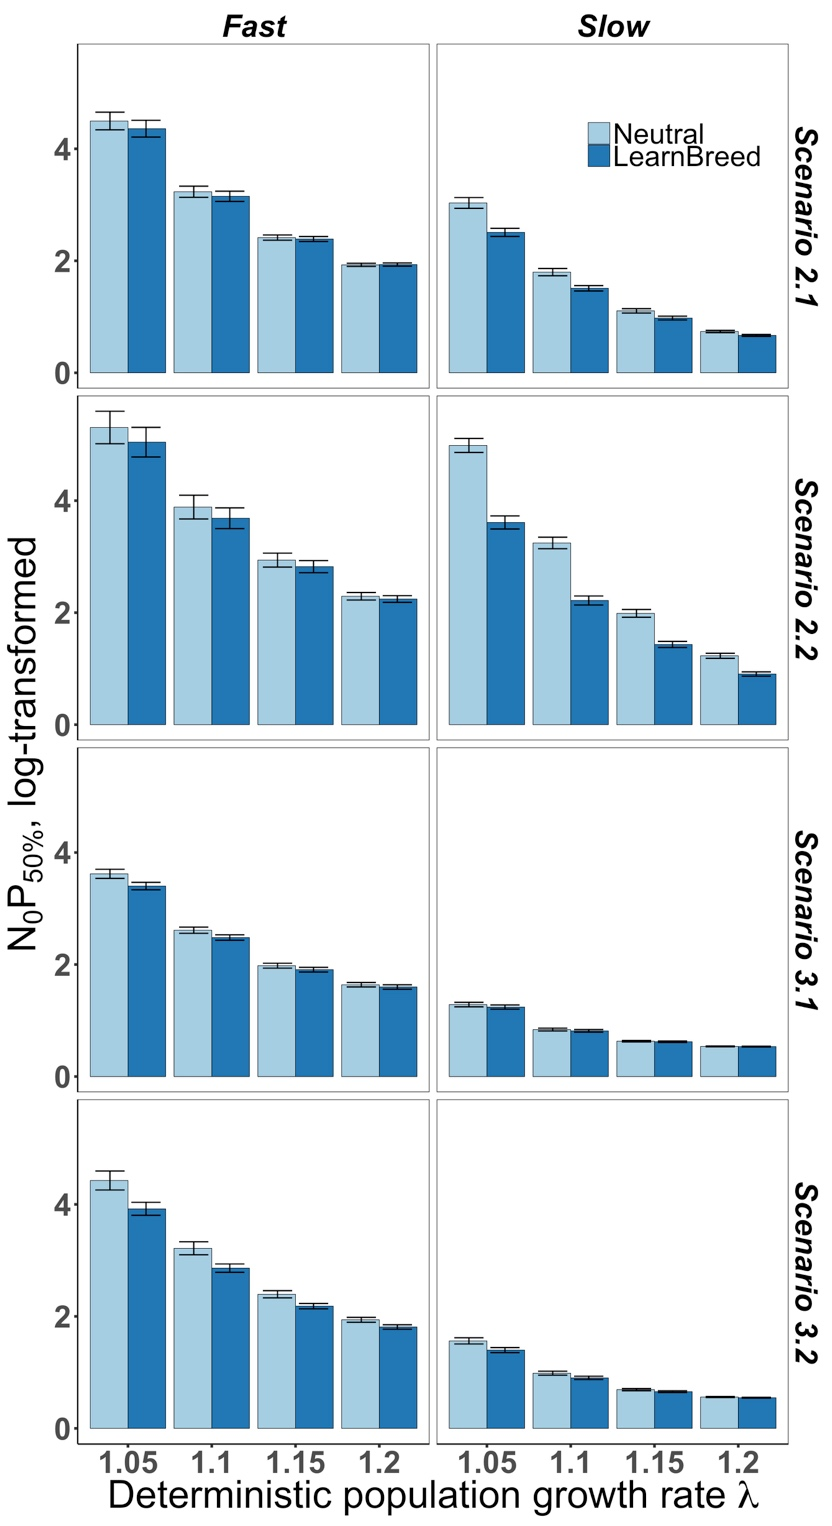
\includegraphics[height=.75\textheight]{./Figures/Appendix3_2/Fig_9.jpg}
\caption[Effects of \textit{LearnBreed} on $N_{0}P_{50\%}$]{
Influence of learning from a breeding experience on population persistence in
novel environments as a function of the position of the species along the
fast-slow continuum. Benefits and costs of the behaviour under different
environmental scenarios are reflected in differences in $N_{0}P_{50\%}$ between
simulations where individuals’ decision about changing habitat depends
(\emph{LearnBreed}) or not (\emph{Neutral}) on the success of the past breeding
attempt.}
\label{fig:figApp3.2.9}
\end{figure}

\begin{figure}
\centering
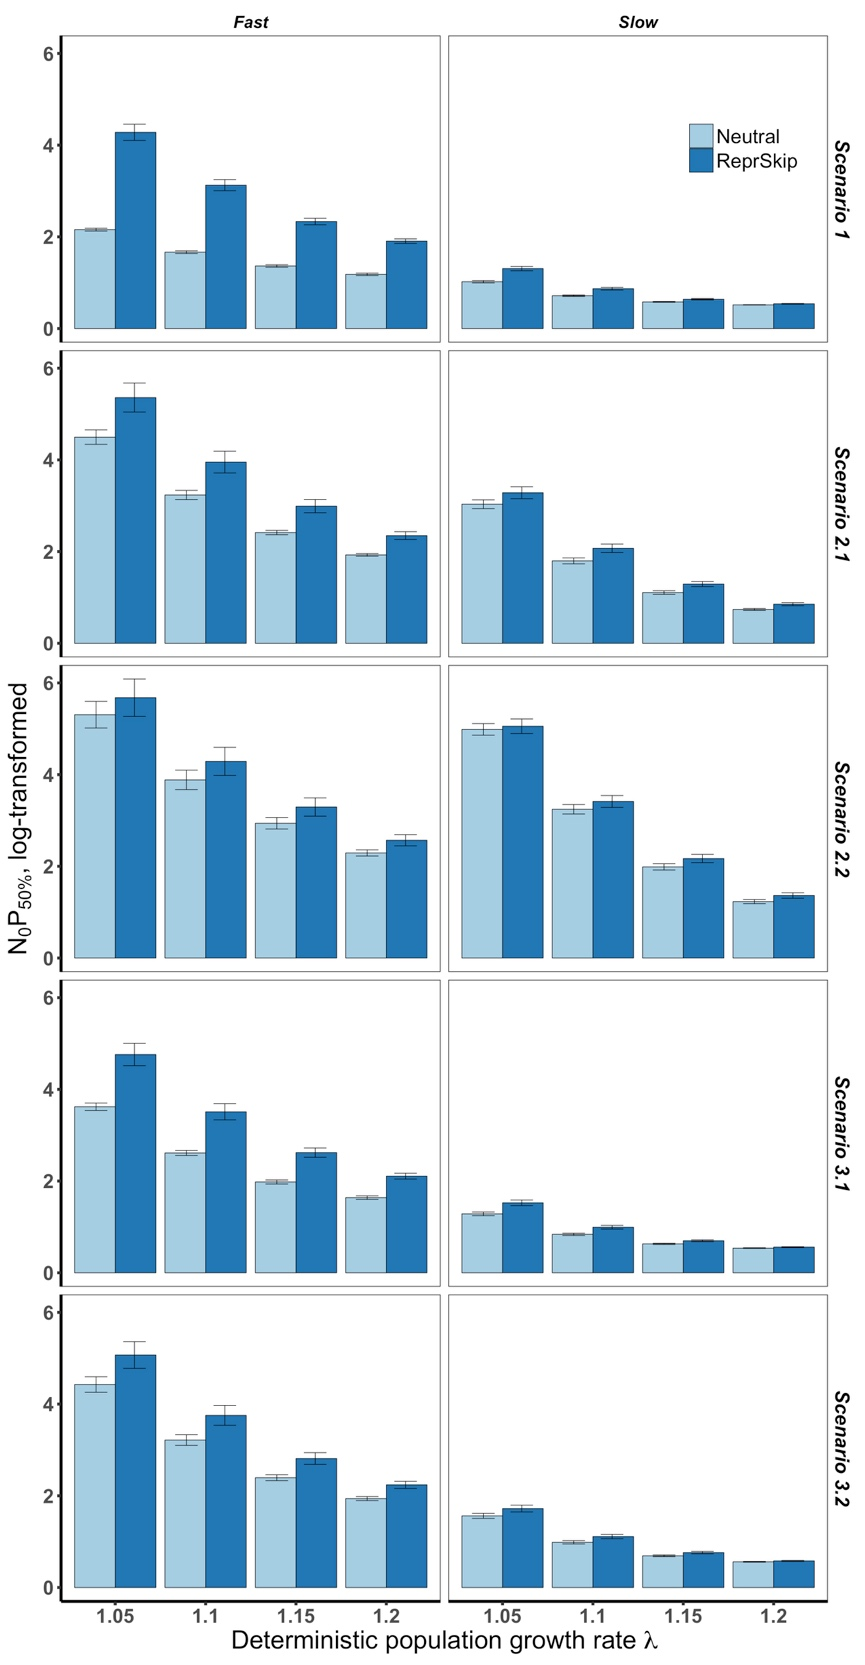
\includegraphics[height=.75\textheight]{./Figures/Appendix3_2/Fig_10.jpg}
\caption[Effects of \textit{ReprSkip} on $N_{0}P_{50\%}$]{
Influence of a reproductive skip on population persistence in novel environments
as a function of the position of the species along the fast-slow continuum.
Benefits and costs of the behaviour under different environmental scenarios are
reflected in differences in $N_{0}P_{50\%}$ between simulations where
individuals either have the option (\emph{ReprSkip}) or not (\{emph{Neutral}) to
skip a reproductive event.}
\label{fig:figApp3.2.10}
\end{figure}

\begin{figure}
\centering
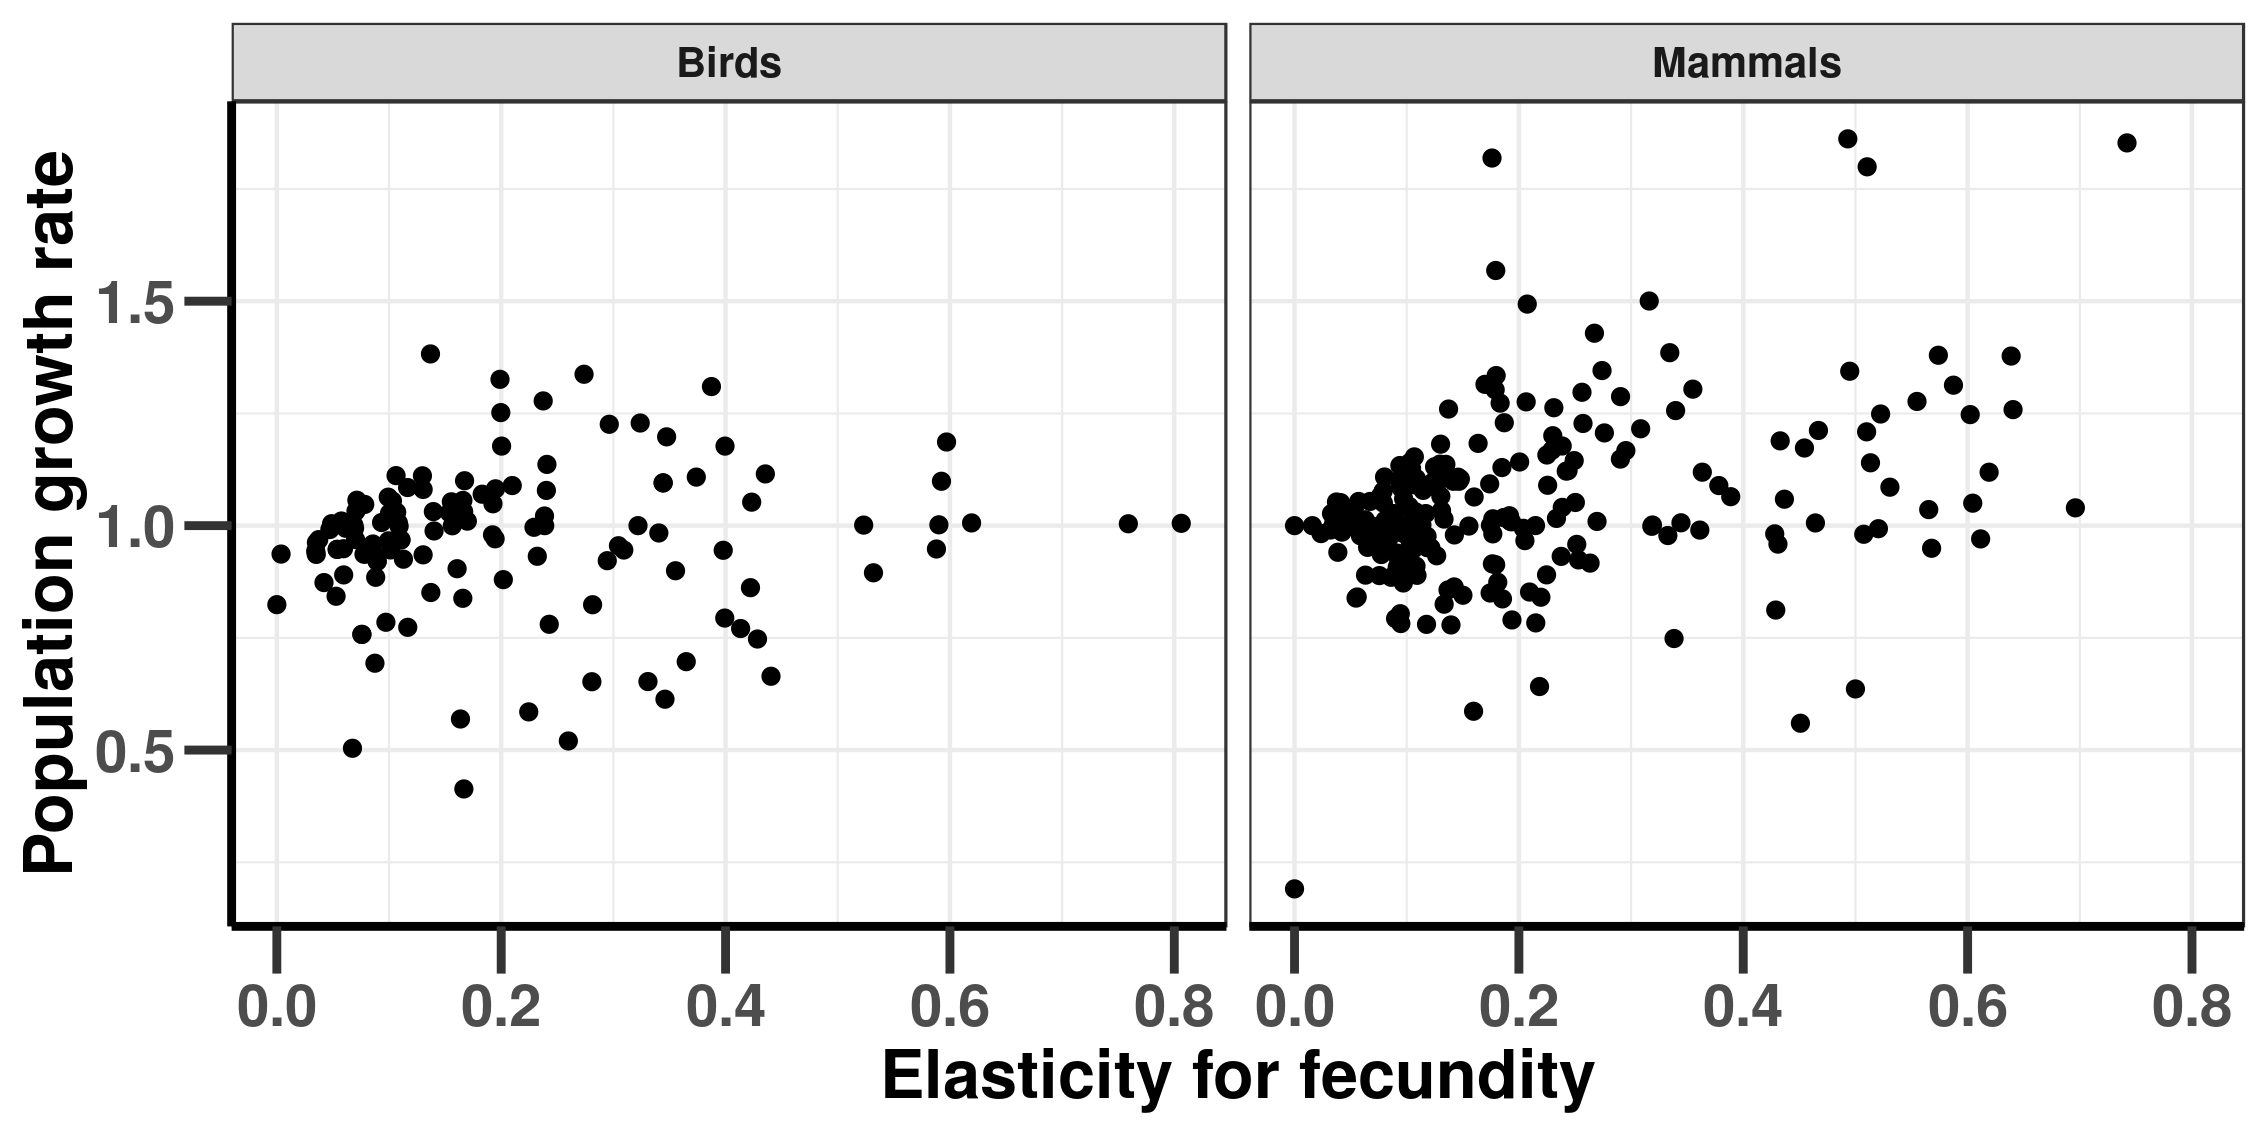
\includegraphics[width=\textwidth]{./Figures/Appendix3_2/Fig_11.png}
\caption[Fast-slow continuum and $\lambda$]{
Relationship between the fast-slow continuum and population grow rate
($\lambda$) in wild populations of birds and mammals suggesting that population
growth rate is not higher for fast-lived strategies than for slow-lived
strategies. Data come from COMADRE \citep{Salguero-Gomez2016}. The fast-slow
continuum is defined as the elasticity of population growth to changes in net
fecundity, based on demographic analysis using the popbio R-package
\cite{Stubben2007}.}
\label{fig:figApp3.2.11}
\end{figure}


%************************************************
\chapter[Appendix 4: Chapter 4 - Supplementary materials]{Appendix 4: Chapter 4
- Supplementary materials}\label{ch:POLS_appendix}
%************************************************
\renewcommand{\thefigure}{A.4.\arabic{figure}}
\setcounter{figure}{0}

\renewcommand{\thetable}{A.4.\arabic{table}}
\setcounter{table}{0}

\section*{Supplementary tables}

\begin{table}[ht!]
\centering
\caption[Intra-class correlation coefficients]{
Gaussian BPMMs used to estimate intra-class correlation coefficients for
variation in FID (log-transformed).}\label{tab:tabApp4.1}
\begin{tabular}{llllll}
\toprule
\multicolumn{6}{@{}l@{}}{\textbf{Model for all observations (n = 11,852 observations of 317 species)}}        \\
\midrule
             & \textbf{post mean} & \textbf{L-95\% CI} & \textbf{U-95\%} & \textbf{eff.samp} & \textbf{pMCMC} \\
\multicolumn{6}{@{}l@{}}{\textbf{Random effects}}                                                   \\
Phylogeny            & 0.299          & 0.172          & 0.451    & 1000       & -                  \\
Species              & 0.222          & 0.163          & 0.274    & 890.6      & -                  \\
Residual             & 0.263          & 0.256          & 0.269    & 1151       & -                  \\
\multicolumn{6}{@{}l@{}}{\textbf{Fixed effects}}                                                    \\
Intercept            & 3.238          & 2.780          & 3.675    & 1000       & \textless{0.001}   \\
\noalign{\bigskip}
\toprule
\multicolumn{6}{@{}l@{}}{\textbf{Model for rural observations (n = 7,373 observations of 303 species)}}       \\
\midrule
             & \textbf{post mean} & \textbf{L-95\% CI} & \textbf{U-95\%} & \textbf{eff.samp} & \textbf{pMCMC} \\
\multicolumn{6}{@{}l@{}}{\textbf{Random effects}}                                                   \\
Phylogeny            & 0.316          & 0.178          & 0.465    & 1000       & -                  \\
Species              & 0.187          & 0.135          & 0.247    & 1585       & -                  \\
Residual             & 0.230          & 0.223          & 0.238    & 638.2      & -                  \\
\multicolumn{6}{@{}l@{}}{\textbf{Fixed effects}}                                                    \\
Intercept            & 3.348          & 2.924          & 3.801    & 1201       & \textless{0.001}   \\
\noalign{\bigskip}
\toprule
\multicolumn{6}{@{}l@{}}{\textbf{Model for urban observations (n = 4479 observations of 108 species)}}        \\
\midrule
             & \textbf{post mean} & \textbf{L-95\% CI} & \textbf{U-95\%} & \textbf{eff.samp} & \textbf{pMCMC} \\
\multicolumn{6}{@{}l@{}}{\textbf{Random effects}}                                                   \\
Phylogeny            & 0.249          & 0.065          & 0.477    & 1000       & -                  \\
Species              & 0.127          & 0.055          & 0.215    & 1000       & -                  \\
Residual             & 0.173          & 0.166          & 0.180    & 1000       & -                  \\
\multicolumn{6}{@{}l@{}}{\textbf{Fixed effects}}                                                    \\
Intercept            & 2.491          & 2.050          & 2.955    & 1000       & \textless{0.001}
\end{tabular}
\end{table}


\begin{table}
\centering
\caption[Best FID models for areas with rural and urban observations]{
Gaussian BPMMs accounting for variation in FID (log-transformed) as a
function of habitat, based on information from regions for which both urban and
rural FID observations were available (Denmark, France, Norway and China). The
model below includes only species for which FIDs were recorded for both urban
and rural habitats.}\label{tab:tabApp4.2}
\begin{tabular}{llllll}
\toprule
\multicolumn{6}{@{}l@{}}{\textbf{Model for all observations (n = 11,852 observations of 317 species)}}     \\
\midrule
          & \textbf{post mean} & \textbf{L-95\% CI} & \textbf{U-95\%} & \textbf{eff.samp} & \textbf{pMCMC} \\
\multicolumn{6}{@{}l@{}}{\textbf{Random effects}}                                         \\
Phylogeny         & 0.424        & 0.205        & 0.656  & 871      & -                   \\
Species           & 0.132        & 0.064        & 0.192  & 1000     & -                   \\
Country           & 0.133        & 0.011        & 0.459  & 1000     & -                   \\
Residual          & 0.204        & 0.198        & 0.209  & 1000     & -                   \\
\multicolumn{6}{@{}l@{}}{\textbf{Fixed effects}}                                          \\
Intercept         & 3.069        & 2.519        & 3.719  & 1000     & \textless{0.001}    \\
Habitat:urban     & -0.397       & -0.417       & -0.377 & 1222     & \textless{0.001}    \\
Height            & 0.017        & 0.014        & 0.020  & 1000     & \textless{0.001}    \\
\noalign{\bigskip}
\toprule
\multicolumn{6}{@{}l@{}}{\textbf{Model for species present in both urban and rural habitats (9266 observations of 246 species)}} \\
\midrule
          & \textbf{post mean} & \textbf{L-95\% CI} & \textbf{U-95\%} & \textbf{eff.samp} & \textbf{pMCMC} \\
\multicolumn{6}{@{}l@{}}{\textbf{Random effects}}                                          \\
Phylogeny         & 0.204        & 0.080        & 0.346  & 1000     & -                    \\
Species           & 0.098        & 0.050        & 0.151  & 1000     & -                    \\
Country           & 0.174        & 0.010        & 0.513  & 596      & -                    \\
Residual          & 0.204        & 0.198        & 0.209  & 1093     & -                    \\
\multicolumn{6}{@{}l@{}}{\textbf{Fixed effects}}                                           \\
Intercept         & 2.854        & 2.343        & 3.415  & 1182     & \textless{0.001}     \\
Habitat:urban     & -0.400       & -0.423       & -0.380 & 906      & \textless{0.001}     \\
Height            & 0.016        & 0.013        & 0.020  & 1000     & \textless{0.001}
\end{tabular}
\end{table}


\begin{table}
\centering
\caption[Best FID models]{Gaussian BPMM accounting for variation in FID 
(log-transformed) as a
function of the fast-slow continuum, based on information from all regions
(11,392 observations belonging to 246 species).}\label{tab:tabApp4.3}
\begin{tabular}{lllllllllll}
\toprule
        & \textbf{post mean} & \textbf{L-95\% CI} & \textbf{U-95\%} & \textbf{eff.samp} & \textbf{pMCMC} \\
\multicolumn{6}{@{}l@{}}{\textbf{Random effects}}                                          \\
Animal             & 0.238         & 0.118        & 0.358  & 1791     & -                  \\
Species            & 0.153         & 0.103        & 0.202  & 1000     & -                  \\
Country            & 0.113         & 0.020        & 0.307  & 1118     & -                  \\
Residual           & 0.209         & 0.204        & 0.214  & 1000     & -                  \\
\multicolumn{6}{@{}l@{}}{\textbf{Fixed effects}}                                           \\
Intercept          & 3.192         & 2.694        & 3.655  & 1000     & \textless{0.001}   \\
FS                 & 0.019         & 0.008        & 0.030  & 1074     & \textless{0.001}   \\
Habitat:urban      & -0.403        & -0.424       & -0.382 & 1000     & \textless{0.001}   \\
Height             & 0.014         & 0.011        & 0.017  & 1000     & \textless{0.001}
\end{tabular}
\end{table}


\begin{table}
\caption[FID model with brain size for rural habitats]{Gaussian BPMM accounting 
for variation in FID (log-transformed) in
rural habitats as a function of residual brain size, based on information from
all regions (3297 observations of 105 species). We restricted the analysis to
rural habitats as previous work suggests that large-brained birds are
over-represented in urbanised environments.}\label{tab:tabApp4.4}
\begin{tabular}{llllll}
\toprule
                    & \textbf{post mean} & \textbf{L-95\% CI} & \textbf{U-95\%} & \textbf{eff.samp} & \textbf{pMCMC} \\
\multicolumn{6}{@{}l@{}}{\textbf{Random effects}}                                          \\
Phylogeny           & 0.290          & 0.136        & 0.480  & 1000     & -                \\
Species             & 0.112          & 0.051        & 0.174  & 1000     & -                \\
Residual            & 0.242          & 0.231        & 0.253  & 1000     & -                \\
\multicolumn{6}{@{}l@{}}{\textbf{Fixed effects}}                                           \\
Intercept           & 3.135          & 2.701        & 3.635  & 827.9    & \textless{0.001} \\
Brain residual      & 0.667          & 0.260        & 1.132  & 1020.6   & 0.008            \\
Height              & 0.010          & 0.003        & 0.017  & 1000     & 0.014
\end{tabular}
\end{table}


\begin{table}
\caption[FID model with brain size for species in rural and urban habitats]{
Gaussian BPMM accounting for across species differences in FID from rural and
urban habitats (response variable) as a function of residual brain size, based
on information from species for which both urban and rural FID observations
were available. The decline of each species was estimated as the log(mean
FIDrural)- log(mean FIDurban). The model was repeated again restricting
the species to those with at least 15 FID observations in each habitat. The
models were run with a Gaussian structure of the errors and non-informative
priors. We weighted the observations by 1/( n-3), being “n” the number of FID
observations of the species.}\label{tab:tabApp4.5}
\begin{tabular}{llllll}
\toprule
\multicolumn{6}{@{}l@{}}{\textbf{Model for all observation (71 species)}}                                  \\
\midrule
          & \textbf{post mean} & \textbf{L-95\% CI} & \textbf{U-95\%} & \textbf{eff.samp} & \textbf{pMCMC} \\
\multicolumn{6}{@{}l@{}}{\textbf{Random effects}}                                                \\
Phylogeny           & 0.228             & 0.085          & 0.390    & 975        & -             \\
Residual            & 0.040             & 0.007          & 0.082    & 975        & -             \\
\multicolumn{6}{@{}l@{}}{\textbf{Fixed effects}}                                                 \\
Intercept           & 0.837             & 0.429          & 1.300    & 975        & 0.002         \\
Brain residual      & 0.160             & -0.296         & 0.694    & 975        & 0.545         \\
\noalign{\bigskip}
\toprule
\multicolumn{6}{@{}l@{}}{\textbf{Model with  species with at least 15 FID observations per hábitat (34 species)}} \\
\midrule
            & \textbf{post mean} & \textbf{L-95\% CI} & \textbf{U-95\%} & \textbf{eff.samp} & \textbf{pMCMC}      \\
\multicolumn{6}{@{}l@{}}{\textbf{Random effects}}                                                     \\
Phylogeny           & 0.154             & 0.059          & 0.258    & 975        & -                  \\
Residual            & 0.010             & 0.000          & 0.027    & 975        & -                  \\
\multicolumn{6}{@{}l@{}}{\textbf{Fixed effects}}                                                      \\
Intercept           & 0.867             & 0.471          & 1.281    & 975        & \textless{0.001}   \\
Brain residual      & 0.162             & -0.315         & 0.690    & 975        & 0.539
\end{tabular}
\end{table}
\clearpage

\section*{Supplementary figures}

\begin{figure}[ht!]
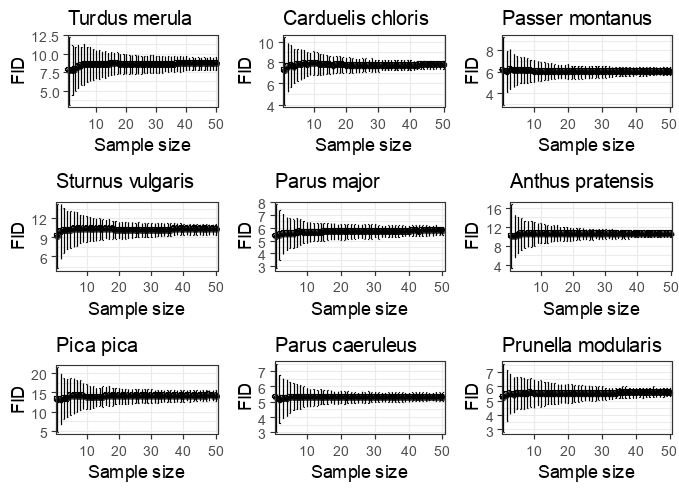
\includegraphics[width=\textwidth]{./Figures/Appendix4_1/Fig_1.png}
\caption[Effects of the sample size on FID estimates]{
Simulations to estimate the minimum sample size needed to accurately estimate
FID. See main text for details.}\label{fig:figApp4.1}
\end{figure}


\begin{figure}
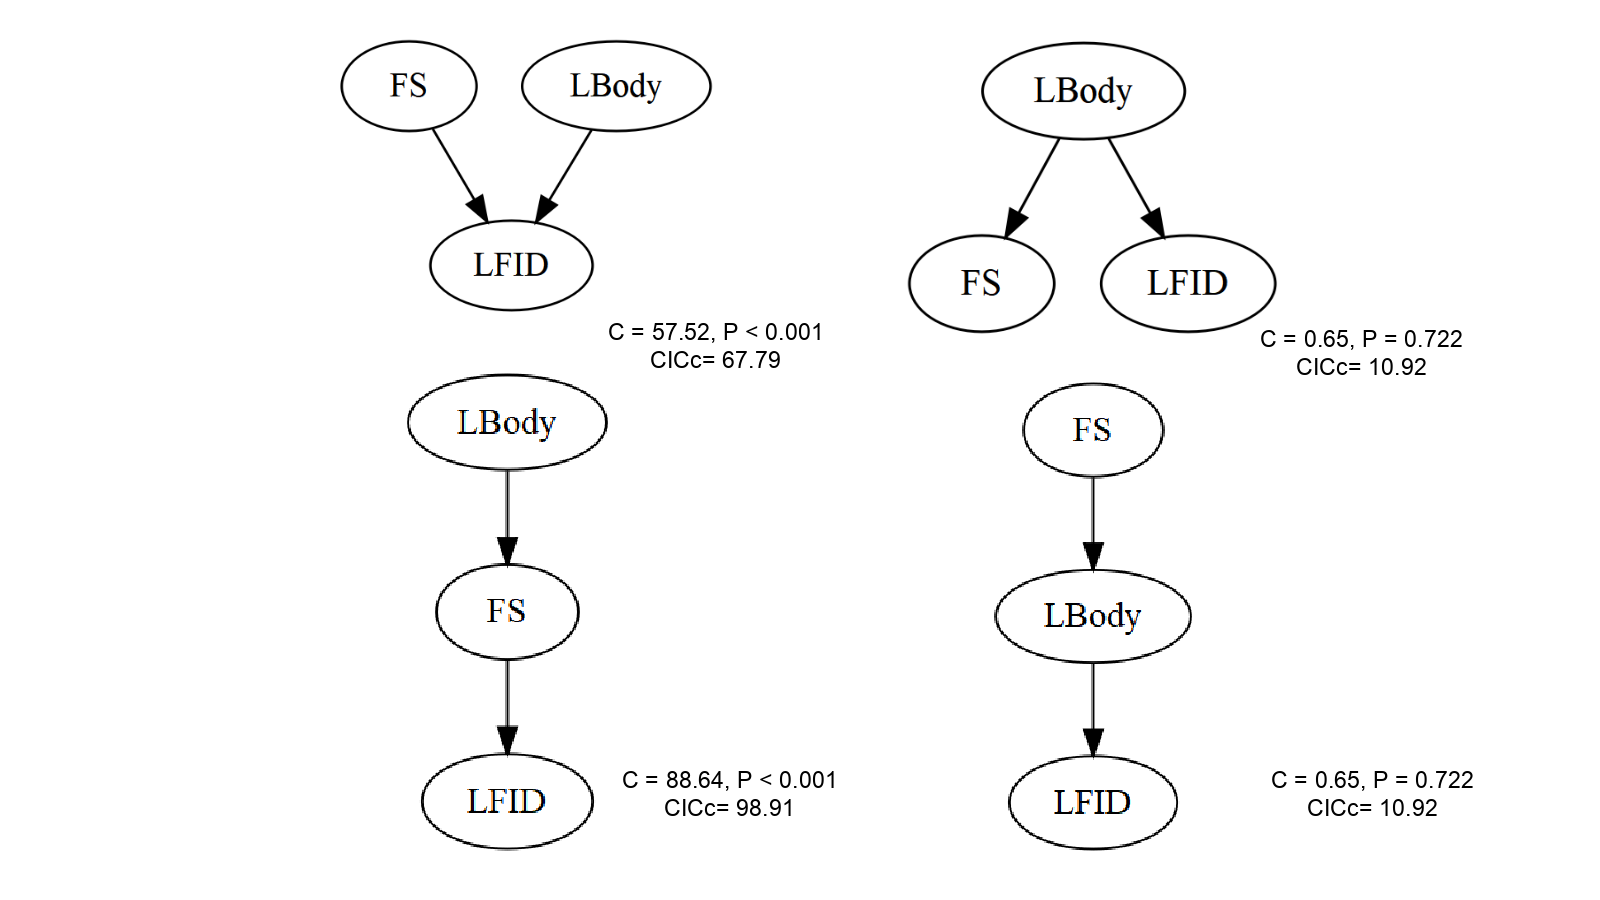
\includegraphics[width=\textwidth]{./Figures/Appendix4_1/Fig_2.png}
\caption[Path analysis with body size for rural habitats]{
Path diagrams of the causal scenarios analysed to study how body size affects
the relationship between flight initiation distance (FID) and the fast-slow
continuum (FS) in rural habitats. The letter “L” before body and FID
denotes log-transformation.}\label{fig:figApp4.2}
\end{figure}


\begin{figure}
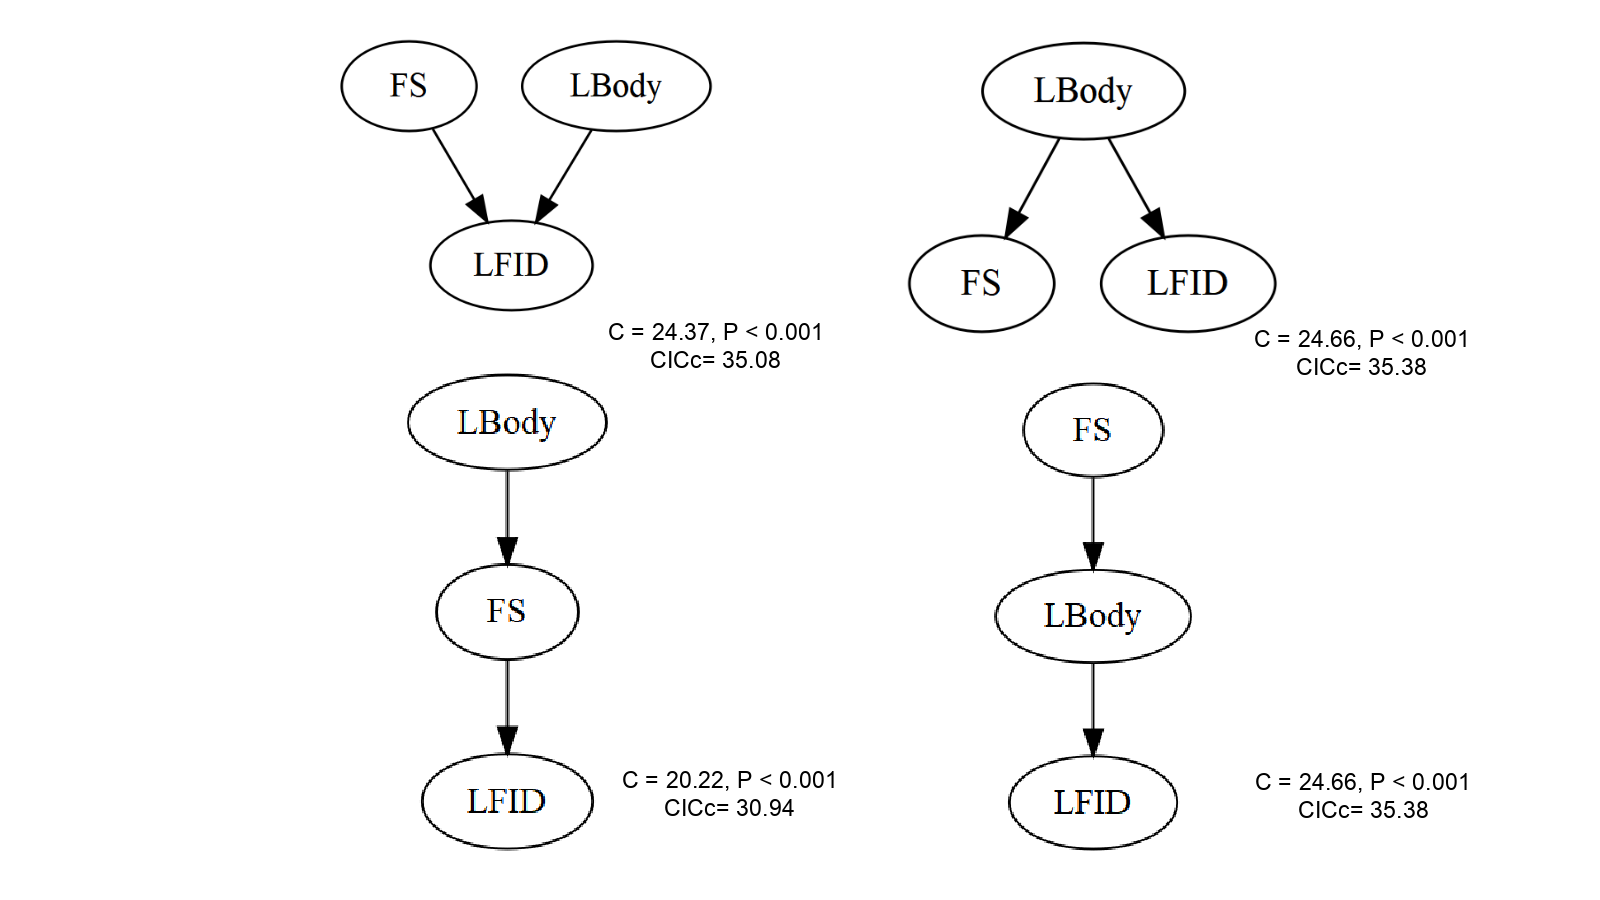
\includegraphics[width=\textwidth]{./Figures/Appendix4_1/Fig_3.png}
\caption[Path analysis with body size for urban habitats]{
Path diagrams of the causal scenarios analysed to study how body size affects
the FID-FS association in urban habitats. The letter “L” before body and
FID denotes log-transformation.}\label{fig:figApp4.3}
\end{figure}


% \include{Chapters/Appendix_5_1}

% \include{Chapters/Appendix_6_1}

%----------------------------------------------------------------------------------------
%	BIBLIOGRAPHY
%----------------------------------------------------------------------------------------

% References - set bibliography style
\bibliographystyle{amnat}
%\bibliographystyle{plainnat} % Use the plainnat bibliography style

% create reference list
\bibliography{library}


%----------------------------------------------------------------------------------------
%	INDEX
%----------------------------------------------------------------------------------------

% \printindex % Print the index

%----------------------------------------------------------------------------------------

\end{document}
